\documentclass[10pt]{article}
\usepackage[verbose, a4paper, hmargin=2.5cm, vmargin=2.5cm]{geometry}

\usepackage{fontspec}
\usepackage{ctex}
\usepackage{paratype}

\usepackage{amsmath}
\usepackage{amssymb}
\usepackage{amsfonts}
\usepackage{esint}
\usepackage{stmaryrd}

\usepackage[mathbf=sym]{unicode-math}
\setmainfont{STIX Two Text}
\setmathfont{STIX Two Math}

\setsansfont{Arial}
\setmonofont{Courier New}

\usepackage{makecell}
\usepackage{wasysym}
\usepackage{pifont}
\usepackage[export]{adjustbox}
\usepackage{graphicx}
\usepackage{mdframed}
\usepackage{booktabs,array,multirow}
\usepackage{tabularx}
\usepackage{hyperref}
\hypersetup{colorlinks=true, linkcolor=blue, filecolor=magenta, urlcolor=cyan,}
\urlstyle{same}
\usepackage[most]{tcolorbox}
\definecolor{mygray}{RGB}{240,240,240}
\tcbset{
  colback=mygray,
  boxrule=0pt,
}
\graphicspath{ {./images/} }
\newcommand{\HRule}{\begin{center}\rule{0.9\linewidth}{0.2mm}\end{center}}
\newcommand{\customfootnote}[1]{
  \let\thefootnote\relax\footnotetext{#1}
}
\newcommand{\lt}{\mathrel{<}}
\newcommand{\gt}{\mathrel{>}}
\newcommand*\circled[1]{\tikz[baseline=(char.base)]{\node[shape=circle,draw,inner sep=1.5pt] (char) {\small #1};}}
\setcounter{MaxMatrixCols}{256}
\begin{document}
2025 版上海高考真题及模拟训练合集(下册)

\section*{口六、解析几何}

板块一:中档客观题

\section*{1. 真题回顾}

A、几何与定义

【例题】1. (2025 上海春考) 已知双曲线 \(\frac{{x}^{2}}{{a}^{2}} - \frac{{y}^{2}}{6 - {a}^{2}} = 1\left( {a > 0}\right)\) 的左，右焦点分别为 \({F}_{1},{F}_{2}\) . 通过 \({F}_{2}\) 且倾斜角为 \(\frac{\pi }{3}\) 的直线与双曲线交于第一象限的点 \(A\) ，延长 \(A{F}_{2}\) 至 \(B\) 使得 \({AB} = {A{F}_{1}}\) . 若 \(\bigtriangleup B{F}_{1}{F}_{2}\) 的面积为 \(3\sqrt{6}\) ，则 \(a\) 的值为\_\_\_\_\_.

【答案】 \(\sqrt{3}\)

【解析】由题意,可得 \(c = \sqrt{6},\left| {{F}_{1}{F}_{2}}\right|  = 2\sqrt{6}\) .

由双曲线的定义得 \({2a} = \left| {A{F}_{1}}\right|  - \left| {A{F}_{2}}\right|  = \left| {AB}\right|  - \left| {A{F}_{2}}\right|  = \left| {B{F}_{2}}\right|\) .

又易得 \(\angle B{F}_{2}{F}_{1} = \frac{\pi }{3}\) ，所以 \({S}_{{\Delta B}{F}_{1}{F}_{2}} = \frac{1}{2} \cdot  \left| {{F}_{1}{F}_{2}}\right|  \cdot  \left| {B{F}_{2}}\right|  \cdot  \sin \frac{\pi }{3} = \frac{1}{2} \cdot  2\sqrt{6} \cdot  {2a} \cdot  \frac{\sqrt{3}}{2} = {3\sqrt{6}}\) ，解得 \(a \; = \sqrt{3}\) .

【例题】2. (2021 上海春考) 已知椭圆 \({x}^{2} + \frac{{y}^{2}}{{b}^{2}} = 1\left( {0 < b < 1}\right)\) 的左、右焦点为 \({F}_{1}\text{ 、 }{F}_{2}\) ,以 \(O\) 为顶点， \({F}_{2}\) 为焦点作抛物线交椭圆于 \(P\) ，且 \(\angle {P{F}_{1}{F}_{2}} = {45}^{ \circ  }\) ，则抛物线的准线方程是\_\_\_\_\_.

【答案】 \(x = 1 - \sqrt{2}\)

【解析】设 \({F}_{1}\left( {-c,0}\right) ,{F}_{2}\left( {c,0}\right)\) ,则抛物线 \({y}^{2} = {4cx}\) ,

直线 \(P{F}_{1} : y = x + c\) ,由 \(\left\{  \begin{array}{l} {y}^{2} = {4cx} \\  y = x + c \end{array}\right.\) ,解得 \(x = c,y = {2c}\) ,

所以点 \(P\) 的坐标为 \(\left( {c,{2c}}\right)\) ,所以 \(P{F}_{2} \bot  {F}_{1}{F}_{2}\) ,又 \(P{F}_{2} = {F}_{2}{F}_{1} = {2c}\) ,所以 \(P{F}_{1} = 2\sqrt{2}c\) 所以 \(P{F}_{1} + \; P{F}_{2} = \left( {2\sqrt{2} + 2}\right) c = {2a} = 2\) ,则 \(c = \sqrt{2} - 1\) ,

所以抛物线的准线方程为 \(x =  - c = 1 - \sqrt{2}\) .

【例题】3. (2021 上海秋考) 已知抛物线 \({y}^{2} = {2px}\left( {p > 0}\right)\) ，若第一象限的 \(A\) 、 \(B\) 在抛物线上，焦点为 \(F\) ， \(\left| {AF}\right|  = 2,\left| {BF}\right|  = 4,\left| {AB}\right|  = 3\) ，则直线 \({AB}\) 的斜率为\_\_\_\_\_.

【答案】 \(\frac{\sqrt{5}}{2}\)

\begin{center}
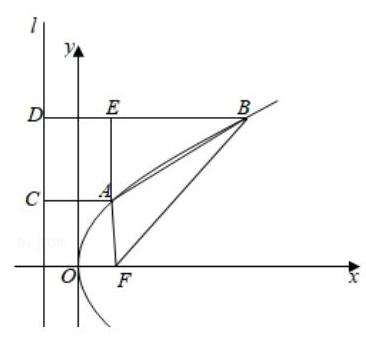
\includegraphics[max width=0.3\textwidth]{images/bo_d5jm9o77aajc7383vmi0_0_1090_1515_366_343_0.jpg}
\end{center}
\hspace*{3em} 

【解析】设抛物线的准线为 \(l\) ,

作 \({AC} \bot  l\) 于点 \(C,{BD} \bot  l\) 于点 \(D,{AE} \bot  {BD}\) 于点 \(E\) ,

由抛物线的定义得 \({AC} = {AF} = 2,{BD} = {BF} = 4\) ,

所以 \({BE} = 4 - 2 = 2,{AE} = \sqrt{A{B}^{2} - B{E}^{2}} = \sqrt{9 - 4} = \sqrt{5}\) ,

所以直线 \({AB}\) 的斜率 \({k}_{AB} = \tan \angle {ABE} = \frac{AE}{BE} = \frac{\sqrt{5}}{2}\) .

【例题】4. (2020 上海秋考) 已知椭圆 \(C : \frac{{x}^{2}}{4} + \frac{{y}^{2}}{3} = 1\) 的右焦点为 \(F\) ,直

线 \(l\) 经过椭圆右焦点 \(F\) ，交椭圆 \(C\) 于 \(P\) 、 \(Q\) 两点(点 \(P\) 在第二象限)，若点 \(Q\) 关于 \(x\) 轴对称点为 \({Q}^{\prime }\) ,且满足 \({PQ} \bot  F{Q}^{\prime }\) ,求直线 \(l\) 的方程是\_\_\_\_\_.

【答案】 \(x + y - 1 = 0\)

【解析】椭圆 \(C : \frac{{x}^{2}}{4} + \frac{{y}^{2}}{3} = 1\) 的右焦点为 \(F\left( {1,0}\right)\) ,

\begin{center}
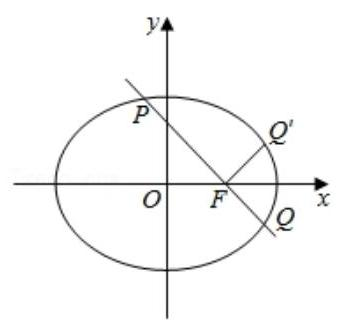
\includegraphics[max width=0.2\textwidth]{images/bo_d5jm9o77aajc7383vmi0_1_1114_232_338_324_0.jpg}
\end{center}
\hspace*{3em} 

直线 \(l\) 经过椭圆右焦点 \(F\) ，交椭圆 \(C\) 于 \(P\) 、 \(Q\) 两点(点 \(P\) 在第二象限),

若点 \(Q\) 关于 \(x\) 轴对称点为 \({Q}^{\prime }\) ，且满足 \({PQ} \bot  F{Q}^{\prime }\) ，

得直线 \(l\) 的斜率为 -1,所以直线 \(l\) 的方程是 \(y =  - \left( {x - 1}\right)\) ,即 \(x + y \; - 1 = 0\) .

【例题】5. (2017 上海春考) 设椭圆 \(\frac{{x}^{2}}{2} + {y}^{2} = 1\) 的左、右焦点分别为 \({F}_{1}\text{ 、 }{F}_{2}\) , 点 \(P\) 在该椭圆上,则使得 \(\bigtriangleup {F}_{1}{F}_{2}P\) 是等腰三角形的点 \(P\) 的个数是\_\_\_\_\_.

【答案】 6

【解析】如图所示, \circled{1} 当点 \(P\) 与短轴的顶点重合时,

\begin{center}
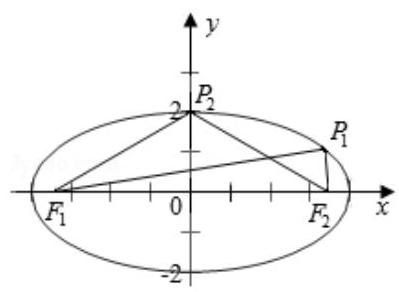
\includegraphics[max width=0.3\textwidth]{images/bo_d5jm9o77aajc7383vmi0_1_1051_722_399_292_0.jpg}
\end{center}
\hspace*{3em} 

\(\bigtriangleup  {F}_{1}{F}_{2}P\) 构成以 \({F}_{1}{F}_{2}\) 为底边的等腰三角形,

此种情况有 2 个满足条件的等腰 \(\bigtriangleup {F}_{1}{F}_{2}P\) ;

 \circled{2}  当 \(\bigtriangleup {F}_{1}{F}_{2}P\) 构成以 \({F}_{1}{F}_{2}\) 为一腰的等腰三角形时,共有 4 个. 以 \({F}_{2}P\) 作为等腰三角形的底边为例,

因为 \({F}_{1}{F}_{2} = {F}_{1}P\) ,所以点 \(P\) 在以 \({F}_{1}\) 为圆心,半径为焦距 \({2c}\) 的圆上,

因此,当以 \({F}_{1}\) 为圆心,半径为 \({2c}\) 的圆与椭圆 \(C\) 有 2 交点时, 存在 2 个满足条件的等腰 \(\bigtriangleup {F}_{1}{F}_{2}P\) .

同理可得当以 \({F}_{2}\) 为圆心,半径为 \({2c}\) 的圆与椭圆 \(C\) 有 2 交点时,

存在 2 个满足条件的等腰 \(\bigtriangleup {F}_{1}{F}_{2}P\) .

综上,满足条件的使得 \(\bigtriangleup {F}_{1}{F}_{2}P\) 是等腰三角形的点 \(P\) 的个数为 6 .

\section*{B、轨迹方程}

【例题】1. (2020 上海春考) 已知椭圆 \(\frac{{x}^{2}}{2} + {y}^{2} = 1\) ，作垂直于 \(x\) 轴的垂线交椭圆于 \(A\) 、 \(B\) 两点，作垂直于 \(y\) 轴的垂线交椭圆于 \(C\) 、 \(D\) 两点，且 \({AB} = {CD}\) ，两垂线相交于点 \(P\) ，则点 \(P\) 的轨迹是 ( )

\begin{center}
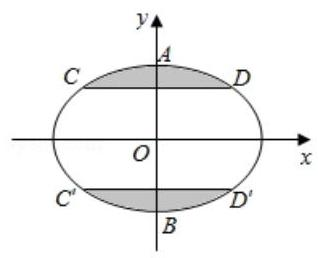
\includegraphics[max width=0.2\textwidth]{images/bo_d5jm9o77aajc7383vmi0_1_1131_1366_318_258_0.jpg}
\end{center}
\hspace*{3em} 

A. 椭圆 B. 双曲线

C. 圆 D. 抛物线

【答案】 \(B\)

【解析】因为 \({AB} \leq  2\) ,所以 \({CD} \leq  2\) ,判断轨迹为上下两支,即选双曲线, 设 \(A\left( {m,t}\right) ,D\left( {t,n}\right)\) ,所以 \(P\left( {m,n}\right)\) ,

因为 \(\frac{{m}^{2}}{2} + {t}^{2} = 1,\frac{{t}^{2}}{2} + {n}^{2} = 1\) ,消去 \(t\) 得 \(2{n}^{2} - \frac{{m}^{2}}{2} = 1\) ,故选 \(B\) .

【例题】2. (2019 上海春考) 以 \(\left( {{a}_{1},0}\right) ,\left( {{a}_{2},0}\right)\) 为圆心的两圆均过 \(\left( {1,0}\right)\) ,与 \(y\) 轴正半轴分别交于 \((0\) , \(\left. {y}_{1}\right) ,\left( {0,{y}_{2}}\right)\) ,且满足 \(\ln {y}_{1} + \ln {y}_{2} = 0\) ,则点 \(\left( {\frac{1}{{a}_{1}},\frac{1}{{a}_{2}}}\right)\) 的轨迹是 ( )

A. 直线 B. 圆 C. 椭圆 D. 双曲线

【答案】 \(A\)

【解析】因为 \({r}_{1} = \left| {1 - {a}_{1}}\right|  = \sqrt{{a}_{1}^{2} + {y}_{1}^{2}}\) ,则 \({y}_{1}^{2} = 1 - 2{a}_{1}\) ,同理可得 \({y}_{2}^{2} = 1 - 2{a}_{2}\) , 又因为 \(\ln {y}_{1} + \ln {y}_{2} = 0\) ,所以 \({y}_{1}{y}_{2} = 1\) ,则 \(\left( {1 - 2{a}_{1}}\right) \left( {1 - 2{a}_{2}}\right)  = 1\) ,

即 \(2{a}_{1}{a}_{2} = {a}_{1} + {a}_{2}\) ,则 \(\frac{1}{{a}_{1}} + \frac{1}{{a}_{2}} = 2\) ,设 \(\left\{  \begin{array}{l} x = \frac{1}{{a}_{1}} \\  y = \frac{1}{{a}_{2}} \end{array}\right.\) ,则 \(x + y = 2\) 为直线,故选 \(A\) .

【例题】3. (2016 上海春考) 对于椭圆 \({C}_{\left( a,b\right) } : \frac{{x}^{2}}{{a}^{2}} + \frac{{y}^{2}}{{b}^{2}} = 1\left( {a,b > 0,a \neq  b}\right)\) . 若点 \(\left( {{x}_{0},{y}_{0}}\right)\) 满足 \(\frac{{x}_{0}^{2}}{{a}^{2}} + \; \frac{{y}_{0}^{2}}{{b}^{2}} < 1\) . 则称该点在椭圆 \({C}_{\left( a,b\right) }\) 内,在平面直角坐标系中,若点 \(A\) 在过点 \(\left( {2,1}\right)\) 的任意椭圆 \({C}_{\left( a,b\right) }\) 内或椭圆 \({C}_{\left( a,b\right) }\) 上,则满足条件的点 \(A\) 构成的图形为 ( )

A. 三角形及其内部 B. 矩形及其内部

C. 圆及其内部 D. 椭圆及其内部

【答案】 \(B\)

【解析】设点 \(A\left( {{x}_{0},{y}_{0}}\right)\) 在过点 \(P\left( {2,1}\right)\) 的任意椭圆 \({C}_{\left( a,b\right) }\) 内或椭圆 \({C}_{\left( a,b\right) }\) 上,

则 \(\frac{4}{{a}^{2}} + \frac{1}{{b}^{2}} = 1,\frac{{x}_{0}^{2}}{{a}^{2}} + \frac{{y}_{0}^{2}}{{b}^{2}} \leq  1\) ,所以 \(\frac{{x}_{0}^{2}}{{a}^{2}} + \frac{{y}_{0}^{2}}{{b}^{2}} \leq  \frac{4}{{a}^{2}} + \frac{1}{{b}^{2}} = 1\) ,

由椭圆的对称性得点 \(B\left( {-2,1}\right)\) ，点 \(C\left( {-2, - 1}\right)\) ，点 \(D\left( {2, - 1}\right)\) ，都在任意椭圆上，

所以满足条件的点 \(A\) 构成的图形为矩形 \({PBCD}\) 及其内部. 故选 \(B\) .

【例题】4. (2013 上海春考)已知 \(A,B\) 为平面内两个定点，过该平面内动点 \(m\) 作直线 \({AB}\) 的垂线，垂足为 \(N\) . 若 \({\overrightarrow{MN}}^{2} = \lambda \overrightarrow{AN} \cdot  \overrightarrow{NB}\) ,其中 \(\lambda\) 为常数,则动点 \(m\) 的轨迹不可能是 ( )

A. 圆 B. 椭圆 C. 双曲线 D. 抛物线

【答案】 \(D\)

【解析】以 \({AB}\) 所在直线为 \(x\) 轴, \({AB}\) 中垂线为 \(y\) 轴,建立坐标系,

设 \(M\left( {x,y}\right) ,A\left( {-a,0}\right) \text{ 、 }B\left( {a,0}\right)\) ,

因为 \(\overrightarrow{MN}{}^{2} = \lambda \overrightarrow{AN} \cdot  \overrightarrow{NB}\) ,所以 \({y}^{2} = \lambda \left( {x + a}\right) \left( {a - x}\right)\) ,

即 \(\lambda {x}^{2} + {y}^{2} = \lambda {a}^{2}\) ,当 \(\lambda  = 1\) 时,轨迹是圆.

当 \(\lambda  > 0\) 且 \(\lambda  \neq  1\) 时,是椭圆的轨迹方程;

当 \(\lambda  < 0\) 时,是双曲线的轨迹方程.

当 \(\lambda  = 0\) 时,是直线的轨迹方程;

综上,方程不表示抛物线的方程. 故选 \(D\) .

C、极限思想(极端原理)

【例题】1. (2022 上海春考) 已知 \({P}_{1}\left( {{x}_{1},{y}_{1}}\right) ,{P}_{2}\left( {{x}_{2},{y}_{2}}\right)\) 两点均在双曲线 \(\Gamma  : \frac{{x}^{2}}{{a}^{2}} - {y}^{2} = 1\left( {a > 0}\right)\) 的右支上，若 \({x}_{1}{x}_{2} > {y}_{1}{y}_{2}\) 恒成立，则实数 \(a\) 的取值范围为\_\_\_\_\_.

【答案】 \(a \geq  1\)

\begin{center}
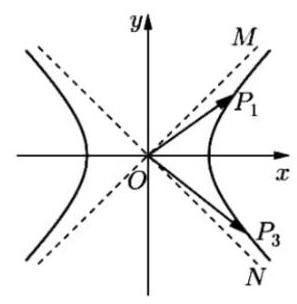
\includegraphics[max width=0.2\textwidth]{images/bo_d5jm9o77aajc7383vmi0_2_1068_1807_297_304_0.jpg}
\end{center}
\hspace*{3em} 

【解析】法一: 设 \({P}_{3}\left( {{x}_{2}, - {y}_{2}}\right)\) ,则 \(\overrightarrow{O{P}_{1}} \cdot  \overrightarrow{O{P}_{3}} = {x}_{1}{x}_{2} - {y}_{1}{y}_{2} > 0\) ,所以 \(\angle {P}_{1}O{P}_{3}\) 恒为锐角,

数形结合,只要两条渐近线的夹角小于等于 \({90}^{ \circ  }\) 即可, 所以其中一条渐近线 \(y = \frac{1}{a}x\) 的斜率 \(\frac{1}{a} \leq  1\) ，所以 \(a \geq  1\) ； 法二: 任取双曲线 \(\Gamma\) 右支上两个不相同的点 \({P}_{1}\left( {{x}_{1},{y}_{1}}\right) ,{P}_{2} \; \left( {{x}_{2},{y}_{2}}\right)\) ,

都有 \({x}_{1}{x}_{2} - {y}_{1}{y}_{2} > 0\) 成立,即 \(1 - \frac{{y}_{1}{y}_{2}}{{x}_{1}{x}_{2}} > 0\) ,即 \({k}_{O{P}_{1}} \cdot  {k}_{O{P}_{2}} < 1\) 恒成立,

当 \({P}_{1}\left( {{x}_{1},{y}_{1}}\right) ,{P}_{2}\left( {{x}_{2},{y}_{2}}\right)\) 坐标越大时,斜率越大,且趋向于渐近线 (取不到),

故只要渐近线的斜率 \(\frac{1}{a}\) 满足 \(\frac{1}{a} \cdot  \frac{1}{a} \leq  1\) ，所以 \(a \geq  1\) ；

法三:由于双曲线的渐近线为 \(y =  \pm  \frac{1}{a}x\) ，

故对于双曲线右支上的点 \({P}_{1}\left( {{x}_{1},{y}_{1}}\right) ,{P}_{2}\left( {{x}_{2},{y}_{2}}\right)\) ,都有 \(\left| {y}_{1}\right|  < \frac{1}{a}{x}_{1},\left| {y}_{2}\right|  < \frac{1}{a}{x}_{2}\) ,

所以 \(\left| {{y}_{1}{y}_{2}}\right|  < \frac{1}{{a}^{2}}{x}_{1}{x}_{2}\) ,因为 \({x}_{1}{x}_{2} - {y}_{1}{y}_{2} > 0\) 恒成立,

所以 \({x}_{1}{x}_{2} > {y}_{1}{y}_{2}\) 恒成立,所以 \({x}_{1}{x}_{2} \geq  \frac{1}{{a}^{2}}{x}_{1}{x}_{2}\) ,所以 \(a \geq  1\) .

【例题】2. (2019 上海秋考) 已知数列 \(\left\{  {a}_{n}\right\}\) 满足 \({a}_{n} < {a}_{n + 1}\left( {n \in  {N}^{ * }}\right) ,{P}_{n}\left( {n,{a}_{n}}\right) \left( {n \geq  3}\right)\) 均在双曲线 \(\frac{{x}^{2}}{6} - \; \frac{{y}^{2}}{2} = 1\) 上，则 \(\mathop{\lim }\limits_{{n \rightarrow  \infty }}\left| {{P}_{n}{P}_{n + 1}}\right|  =\) \_\_\_\_\_.

【答案】 \(\frac{2\sqrt{3}}{3}\)

【解析】法一: 由 \(\frac{{n}^{2}}{6} - \frac{{a}_{n}^{2}}{2} = 1\) ,得 \({a}_{n} = \sqrt{2\left( {\frac{{n}^{2}}{6} - 1}\right) }\) ,所以 \(P\left( {n,\sqrt{2\left( {\frac{{n}^{2}}{6} - 1}\right) }}\right)\) ,

所以 \({P}_{n + 1}\left( {n + 1,\sqrt{2\left( {\frac{{\left( n + 1\right) }^{2}}{6} - 1}\right) }}\right)\) ,

所以 \(\left| {{P}_{n}{P}_{n + 1}}\right|  = \sqrt{{\left( n + 1 - n\right) }^{2} + {\left\lbrack  \sqrt{2{\left( \frac{n + 1}{6}\right) }^{2} - 1} - \sqrt{2\left( {\frac{{n}^{2}}{6} - 1}\right) }\right\rbrack  }^{2}}\) ,

\(= \sqrt{\frac{2{n}^{2} + {2n} - {11}}{3} - 4\sqrt{\left( {\frac{{\left( n + 1\right) }^{2}}{6} - 1}\right) \left( {\frac{{n}^{2}}{6} - 1}\right) }}\)

所以求解极限得 \(\mathop{\lim }\limits_{{n \rightarrow  \infty }}\left| {{P}_{n}{P}_{n + 1}}\right|  = \frac{2\sqrt{3}}{3}\) ,

法二: 当 \(n \rightarrow   + \infty\) 时, \({P}_{n}{P}_{n + 1}\) 与渐近线平行, \({P}_{n}{P}_{n + 1}\) 在 \(x\) 轴的投影为 1,

渐近线倾斜角为 \(\theta\) ,则 \(\tan \theta  = \frac{\sqrt{3}}{3}\) ,故 \({P}_{n}{P}_{n + 1} = \frac{1}{\cos \frac{\pi }{6}} = \frac{2\sqrt{3}}{3}\) .

【例题】3. (2011 上海秋考) 已知点 \(O\left( {0,0}\right) \text{ 、 }{Q}_{0}\left( {0,1}\right)\) 和点 \({R}_{0}\left( {3,1}\right)\) ,记 \({Q}_{0}{R}_{0}\) 的中点为 \({P}_{1}\) ,取 \({Q}_{0}{P}_{1}\) 和 \({P}_{1}{R}_{0}\) 中的一条,记其端点为 \({Q}_{1}\text{ 、 }{R}_{1}\) ,使之满足 \(\left( {\left| {O{Q}_{1}}\right|  - 2}\right) \left( {\left| {O{R}_{1}}\right|  - 2}\right)  < 0\) ,记 \({Q}_{1}{R}_{1}\) 的中点为 \({P}_{2}\) , 取 \({Q}_{1}{P}_{2}\) 和 \({P}_{2}{R}_{1}\) 中的一条,记其端点为 \({Q}_{2}\text{ 、 }{R}_{2}\) ,使之满足 \(\left( {\left| {O{Q}_{2}}\right|  - 2}\right) \left( {\left| {O{R}_{2}}\right|  - 2}\right)  < 0\) . 依次下去, 得到 \({P}_{1},{P}_{2},\cdots ,{P}_{n},\cdots\) ,则 \(\mathop{\lim }\limits_{{n \rightarrow  \infty }}\left| {{Q}_{0}{P}_{n}}\right|  =\) \_\_\_\_\_.

【答案】 \(\sqrt{3}\)

【解析】由题意得 \(\left( {\left| {O{Q}_{1}}\right|  - 2}\right) \left( {\left| {O{R}_{1}}\right|  - 2}\right)  < 0\) ,所以第一次只能取 \({P}_{1}{R}_{0}\) 一条,

\(\left( {\left| {O{Q}_{2}}\right|  - 2}\right) \left( {\left| {O{R}_{2}}\right|  - 2}\right)  < 0\) . 依次下去,则 \({Q}_{1}\text{ 、 }{R}_{1};{Q}_{2}\text{ 、 }{R}_{2},\cdots\) 中必有一点在 \(\left( {\sqrt{3},1}\right)\)

的左侧，一点在右侧，由于 \({P}_{1},{P}_{2},\cdots {P}_{n},\cdots\) 是中点，

由题意得 \({P}_{1},{P}_{2},\cdots {P}_{n},\cdots\) 的极限为 \(\left( {\sqrt{3},1}\right)\) ,所以 \(\mathop{\lim }\limits_{{n \rightarrow  \infty }}\left| {{Q}_{0}{P}_{n}}\right|  = \left| {{Q}_{0}{P}_{1}}\right|  = \sqrt{3}\) .

\section*{2. 模拟练习}

【练习】1. 若椭圆 \(\frac{{x}^{2}}{{a}^{2}} + \frac{{y}^{2}}{{b}^{2}} = 1\left( {a > b > 0}\right)\) 的右焦点 \(F\left( {c,0}\right)\) 关于直线 \(y = \frac{b}{c}x\) 的对称点 \(Q\) 仍然在椭圆上，则该椭圆的离心率为\_\_\_\_\_. 2025 版上海高考真题及模拟训练合集(下册)

【答案】 \(\frac{\sqrt{2}}{2}\)

【解析】法一: 设椭圆的另一个焦点为 \({F}_{1}\left( {-c,0}\right)\) ,连接 \(Q{F}_{1}\text{ 、 }{QF}\) ,

设 \({QF}\) 与直线 \(y = \frac{b}{c}x\) 交于点 \(M\) ，由题意得 \(M\) 为线段 \({QF}\) 的中点，

所以 \({F}_{1}Q//{OM}\) ,又 \({OM} \bot  {FQ}\) ,所以 \({F}_{1}Q \bot  {QF},\left| {{F}_{1}Q}\right|  = 2\left| {OM}\right|\) ,

在 Rt \(\bigtriangleup {MOF}\) 中, \(\tan \angle {MOF} = \frac{\left| MF\right| }{\left| OM\right| } = \frac{b}{c},\left| {OF}\right|  = c\) ,得 \(\left| {OM}\right|  = \frac{{c}^{2}}{a},\left| {MF}\right|  = \frac{bc}{a}\) ,故 \(\left| {QF}\right|  =\)

\(2\left| {MF}\right|  = \frac{2bc}{a},\left| {Q{F}_{1}}\right|  = 2\left| {OM}\right|  = \frac{2{c}^{2}}{a},\)

\begin{center}
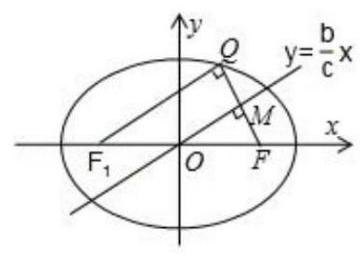
\includegraphics[max width=0.3\textwidth]{images/bo_d5jm9o77aajc7383vmi0_4_1096_618_361_256_0.jpg}
\end{center}
\hspace*{3em} 

由椭圆定义得 \(\left| {QF}\right|  + \left| {Q{F}_{1}}\right|  = \frac{2bc}{a} + \frac{2{c}^{2}}{a} = {2a}\) ,得 \(b = c\) ,

所以 \(a = \sqrt{{b}^{2} + {c}^{2}} = \sqrt{2}c\) ,故 \(\mathrm{e} = \frac{c}{a} = \frac{\sqrt{2}}{2}\) .

法二: 设 \(F\left( {c,0}\right)\) 关于直线 \(y = \frac{b}{c}x\) 的对称点为 \(Q\left( {m,n}\right)\) ,

则有线段 \({FQ}\) 中点坐标为 \(\left( {\frac{m + c}{2},\frac{n}{2}}\right)\) ,且直线 \({FQ}\) 与直线 \(y =\)

\(\frac{b}{c}x\) 垂直,所以有 \(\left\{  \begin{array}{l} \frac{n}{m - c} \cdot  \frac{b}{c} =  - 1 \\  \frac{n}{2} = \frac{b}{c} \times  \frac{m + c}{2} \end{array}\right.\) ,解得 \(m = \frac{{c}^{3} - c{b}^{2}}{{a}^{2}},n = \frac{{2b}{c}^{2}}{{a}^{2}}\) ,

所以 \(Q\left( {\frac{{c}^{3} - c{b}^{2}}{{a}^{2}},\frac{{2b}{c}^{2}}{{a}^{2}}}\right)\) 在椭圆上,即有 \(\frac{{\left( \frac{{c}^{3} - c{b}^{2}}{{a}^{2}}\right) }^{2}}{{a}^{2}} + \frac{{\left( \frac{{2b}{c}^{2}}{{a}^{2}}\right) }^{2}}{{b}^{2}} = 1\) ,

又 \(\mathrm{e} = \frac{c}{a}\) ,得 \({\mathrm{e}}^{2}\left( {4{\mathrm{e}}^{4} - 4{\mathrm{e}}^{2} + 1}\right)  + 4{\mathrm{e}}^{4} = 1\) ,得 \(4{\mathrm{e}}^{6} + {\mathrm{e}}^{2} - 1 = 0\) ,

所以 \(4{\mathrm{e}}^{6} - 2{\mathrm{e}}^{4} + 2{\mathrm{e}}^{4} - {\mathrm{e}}^{2} + 2{\mathrm{e}}^{2} - 1 = 0\) ,即 \(\left( {2{\mathrm{e}}^{2} - 1}\right) \left( {2{\mathrm{e}}^{4} + {\mathrm{e}}^{2} + 1}\right)  = 0\) ,

因为 \(0 < \mathrm{e} < 1\) ，所以 \(2{\mathrm{e}}^{2} - 1 = 0\) ，解得 \(\mathrm{e} = \frac{\sqrt{2}}{2}\) .

【练习】2. (2024 奉贤三模) 若曲线 \(\Gamma  : \frac{{x}^{2}}{{a}^{2}} - {y}^{2} = 1\left( {x > 0}\right)\) 得右顶点 \(A\) ,若对线段 \({OA}\) 上任意一点 \(P\) ,端点除外,在 \(\Gamma\) 上存在关于 \(x\) 轴对称得两点 \(Q\text{ 、 }R\) 使得三角形 \({PQR}\) 为等边三角形,则正数 \(a\) 得取值范围是\_\_\_\_\_.

【答案】 \((0,\sqrt{3}\rbrack\)

【解析】由任意点 \(P\) 线段 \({OA}\) 上,端点除外,在 \(\Gamma\) 上存在关于 \(x\) 轴对称得两点 \(Q,R\) 使得 \(\bigtriangleup {PQR}\) 为等边三角形,

即存在点 \(Q\) 使得 \(\angle {QPx} = {30}^{ \circ  }\) ,所以存在点 \(Q\) 使得 \(\angle {QOx} < {30}^{ \circ  }\) , 由双曲线 \(\Gamma  : \frac{{x}^{2}}{{a}^{2}} - {y}^{2} = 1\left( {x > 0}\right)\) 的其中一条渐近线方程为 \(y = \frac{1}{a}x\) , 则满足 \(y = \frac{1}{a}x\) 的斜率大于或等于 \(\frac{\sqrt{3}}{3}\) ,即 \(\frac{1}{a} \geq  \frac{\sqrt{3}}{3}\) ,所以 \(a \leq  \sqrt{3}\) , 又由 \(a > 0\) ，所以实数 \(a\) 的取值范围为 \((0,\sqrt{3}\rbrack\) .

\begin{center}
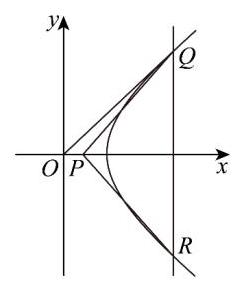
\includegraphics[max width=0.2\textwidth]{images/bo_d5jm9o77aajc7383vmi0_4_1217_1577_233_286_0.jpg}
\end{center}
\hspace*{3em} 

故答案为: \((0,\sqrt{3}\rbrack\) .

【练习】3. 椭圆 \(C : \frac{{x}^{2}}{{a}^{2}} + \frac{{y}^{2}}{{b}^{2}} = 1\left( {a > b > 0}\right)\) 的左、右焦点分别为 \({F}_{1}\text{ 、 }{F}_{2}\) ,点 \(P\) 在椭圆上且同时满足:

 \circled{1}  \(\bigtriangleup  {F}_{1}{F}_{2}P\) 是等腰三角形;  \circled{2}  \(\bigtriangleup  {F}_{1}{F}_{2}P\) 是钝角三角形;  \circled{3} 线段 \({F}_{1}{F}_{2}\) 为 \(\bigtriangleup  {F}_{1}{F}_{2}P\) 的腰;

 \circled{4}  椭圆 \(C\) 上恰好有 4 个不同的点 \(P\) . 则椭圆 \(C\) 的离心率的取值范围是\_\_\_\_\_. 2025 版上海高考真题及模拟训练合集(下册)

【答案】 \(\left( {\frac{1}{3},\sqrt{2} - 1}\right)\)

【解析】如图,不妨设 \(P\) 在第二象限,

由题意得, \(\left| {P{F}_{1}}\right|  = \left| {{F}_{1}{F}_{2}}\right|  = {2c}\) ,则 \(\left| {P{F}_{2}}\right|  = {2a} - {2c}\) ,

由椭圆的对称性,在四个象限内各存在一个满足条件的点 \(P\) ,

\begin{center}
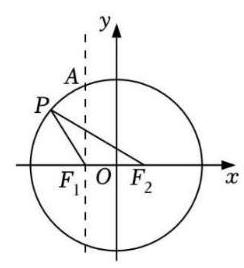
\includegraphics[max width=0.2\textwidth]{images/bo_d5jm9o77aajc7383vmi0_5_1220_441_244_268_0.jpg}
\end{center}
\hspace*{3em} 

在 \(\bigtriangleup  {P{F}_{1}{F}_{2}}\) 中，任意两边之和大于第三边，则 \({4c} > {2a} - {2c}\) ，

所以离心率为 \(\mathrm{e} = \frac{c}{a} > \frac{1}{3}\) ,

过点 \({F}_{1}\) 作直线 \(A{F}_{1}\) 垂直于 \(x\) 轴,与椭圆交于 \(A\) 点,则 \(\left| {A{F}_{1}}\right|  = \frac{{b}^{2}}{a}\) ,

因为 \(\bigtriangleup {F}_{1}{F}_{2}P\) 是钝角三角形,所以 \(\left| {A{F}_{1}}\right|  > \left| {P{F}_{1}}\right|\) ,即 \(\frac{{b}^{2}}{a} > {2c}\) ,得 \({\mathrm{e}}^{2} + 2\mathrm{e} - 1 \; < 0\) ,

解得 \(\mathrm{e} < \sqrt{2} - 1\) ,

综上,椭圆离心率的取值范围为 \(\left( {\frac{1}{3},\sqrt{2} - 1}\right)\) .

【练习】4. 已知直线 \(l\) 的倾斜角为锐角,且过抛物线 \(y = {x}^{2}\) 的焦点,与抛物线交于 \(A\text{ 、 }B\) 两点,若在该抛物线准线上存在一点 \(C\) ,使得 \(\bigtriangleup  {ABC}\) 为正三角形，则直线 \(l\) 的斜率为\_\_\_\_\_.

【答案】 \(\sqrt{2}\)

【解析】法一: 依题意有抛物线 \(y = {x}^{2}\) 的焦点为 \(\left( {0,\frac{1}{4}}\right)\) ,准线方程为 \(y =  - \frac{1}{4}\) ,

设直线 \({AB}\) 的方程为 \(y = {kx} + \frac{1}{4}\left( {k > 0}\right)\) ，代入抛物线的方程 \(y = {x}^{2}\) ，可得 \({x}^{2} - {kx} - \frac{1}{4} = 0\) ，

设 \(A\left( {{x}_{1},{y}_{1}}\right) ,B\left( {{x}_{2},{y}_{2}}\right)\) ,则 \({x}_{1} + {x}_{2} = k,{x}_{1}{x}_{2} =  - \frac{1}{4}\) ,

所以 \({y}_{1} + {y}_{2} = k\left( {{x}_{1} + {x}_{2}}\right)  + \frac{1}{2} = {k}^{2} + \frac{1}{2}\) ,所以 \({AB}\) 的中点为 \(H\left( {\frac{k}{2},\frac{1}{4} + \frac{{k}^{2}}{2}}\right)\) ,

因为在该抛物线的准线上存在一点 \(C\) ,使得 \(\bigtriangleup {ABC}\) 为正三角形,可得 \({CH} \bot  {AB}\) ,且 \(\left| {CH}\right|  = \; \frac{\sqrt{3}}{2}\left| {AB}\right| ,\)

由 \(\left| {AB}\right|  = \sqrt{1 + {k}^{2}} \cdot  \sqrt{{\left( {x}_{1} + {x}_{2}\right) }^{2} - 4{x}_{1}{x}_{2}} = \sqrt{1 + {k}^{2}} \cdot  \sqrt{{k}^{2} + 1} = {k}^{2} + 1\) ,

所以 \(\left| {CH}\right|  = \frac{\sqrt{3}}{2}\left( {{k}^{2} + 1}\right)\) ,设 \(C\left( {{x}_{0}, - \frac{1}{4}}\right)\) ,又 \({CH}\) 的斜率为 \(- \frac{1}{k}\) ,

所以 \(\frac{\frac{{k}^{2}}{2} + \frac{1}{4} + \frac{1}{4}}{\frac{k}{2} - {x}_{0}} =  - \frac{1}{k}\) ,解得 \(C\) 的横坐标为 \({x}_{0} = \frac{{k}^{3}}{2} + k,C\) 的纵坐标为 \(- \frac{1}{4}\) ,

所以 \(\left| {CH}\right|  = \sqrt{{\left( \frac{{k}^{3}}{2} + k - \frac{k}{2}\right) }^{2} + {\left( -\frac{1}{4} - \frac{1}{4} - \frac{{k}^{2}}{2}\right) }^{2}} =\)

\begin{center}
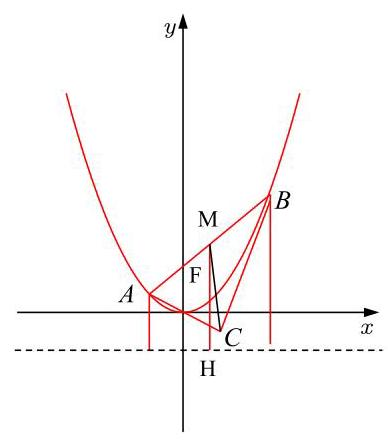
\includegraphics[max width=0.3\textwidth]{images/bo_d5jm9o77aajc7383vmi0_5_1066_1671_388_441_0.jpg}
\end{center}
\hspace*{3em} 

\(\left( {\frac{{k}^{2}}{2} + \frac{1}{2}}\right) \sqrt{{k}^{2} + 1}\)

由 \(\left| {CH}\right|  = \frac{\sqrt{3}}{2}\left| {AB}\right|\) ,可得 \(\frac{\sqrt{3}}{2}\left( {{k}^{2} + 1}\right)  = \left( {\frac{{k}^{2}}{2} + \frac{1}{2}}\right) \sqrt{{k}^{2} + 1}\) ,解

得 \(k = \sqrt{2}\) (舍去负值).

故答案为: \(\sqrt{2}\) .

法二:取 \({AB}\) 中点，作 \({HM} \bot\) 准线于 \(H\)

\({HM} = \frac{1}{2}\left( {{AF} + {BF}}\right)  = {AM}\)

\(\Rightarrow  \frac{HM}{CM} = \frac{AM}{CM} = \frac{1}{\sqrt{3}}\)

\(\Rightarrow  {k}_{AB} = \tan \angle {CMH} = \frac{CH}{MH} = \sqrt{2}\)

【练习】5. (2024 浦东三模) 已知点 \(A\text{ 、 }B\) 位于抛物线 \({y}^{2} = {2px}\left( {p > 0}\right)\) 上， \(\left| {AB}\right|  = {20}\) ，点 \(M\) 为线段 \({AB}\) 的中点，记点 \(M\) 到 \(y\) 轴的距离为 \(d\) . 若 \(d\) 的最小值为 7，则当 \(d\) 取该最小值时，直线 \({AB}\) 的斜率 \(k\left( {k > 0}\right)\) 为\_\_\_\_\_.

【答案】 \(\frac{\sqrt{6}}{2}\)

【解析】如图: 分别从 \(A,B,M\) 作准线的垂线,垂足为 \(C,D,N\) ,

\begin{center}
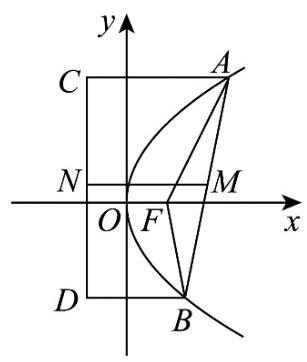
\includegraphics[max width=0.2\textwidth]{images/bo_d5jm9o77aajc7383vmi0_6_1152_633_307_362_0.jpg}
\end{center}
\hspace*{3em} 

设 \(A\left( {{x}_{1},{y}_{1}}\right) ,B\left( {{x}_{2},{y}_{2}}\right) ,{AB}\) 中点 \(M\left( {\frac{{x}_{1} + {x}_{2}}{2},\frac{{y}_{1} + {y}_{2}}{2}}\right)\) ,

\(\left| {MN}\right|  = \frac{1}{2}\left( {\left| {AC}\right|  + \left| {BD}\right| }\right)  = \frac{1}{2}\left( {\left| {AF}\right|  + \left| {BF}\right| }\right)\) ,则 \(M\) 到 \(y\) 轴的距离为 \(d = \; \frac{1}{2}\left( {\left| {AF}\right|  + \left| {BF}\right| }\right)  - \frac{1}{2}p \geq  \frac{1}{2}\left| {AB}\right|  - \frac{1}{2}p = 7,\)

当 \(M\) 到 \(y\) 轴的距离最小时, \(\left| {AF}\right|  + \left| {BF}\right|\) 最小,等号为 \(A,B,F\) 三点共线时取得,所以 \(\frac{1}{2} \times  {20} - \frac{1}{2}p = 7\) ,解得 \(p = 6\) .

故抛物线方程为 \({y}^{2} = {12x}\) ,当 \(A,B,F\) 三点共线时,设直线 \({AB}\) 的方程为 \(y = k\left( {x - 3}\right)\) ,

与抛物线方程联立消去 \(y\) 得: \({k}^{2}{x}^{2} - \left( {6{k}^{2} + {12}}\right) x + 9{k}^{2} = 0\) ,所以 \({x}_{1} + {x}_{2} = \frac{6{k}^{2} + {12}}{{k}^{2}}\) ,

所以 \({x}_{1} + {x}_{2} + p = \frac{6{k}^{2} + {12}}{{k}^{2}} + 6 = {20}\) ,解得 \(k = \frac{\sqrt{6}}{2}\) (负根舍去).

故答案为: \(\frac{\sqrt{6}}{2}\)

【练习】6. (2024 上海三模) 过抛物线 \(E : {y}^{2} = {2px}\left( {p > 0}\right)\) 的焦点 \(F\) 的直线交 \(E\) 于点 \(A,B\) ,交 \(E\) 的准线 \(l\) 于点 \(C,{AD} \bot  l\) ，点 \(D\) 为垂足. 若 \(F\) 是 \({AC}\) 的中点，且 \(\left| {AF}\right|  = 3\) ，则 \(\left| {AB}\right|  =\) \_\_\_\_\_.

【答案】 4

【解析】作 \({BE} \bot  l\) 于点 \(E,l\) 与 \(x\) 轴交于点 \(M\) ,如图,

\begin{center}
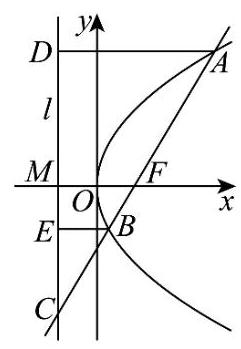
\includegraphics[max width=0.2\textwidth]{images/bo_d5jm9o77aajc7383vmi0_6_1220_1461_241_349_0.jpg}
\end{center}
\hspace*{3em} 

则 \({AD}//{FM}//{BE}\) ，

又 \(\left| {AF}\right|  = 3\) 且 \(F\) 是 \({AC}\) 的中点，则有 \(\frac{\left| AD\right| }{\left| FM\right| } = \frac{\left| AC\right| }{\left| FC\right| } = 2\) ，

即 \(\left| {AD}\right|  = 2\left| {FM}\right|\) ,又 \(\left| {AD}\right|  = \left| {AF}\right|  = 3\) ,故 \(\left| {FM}\right|  = \frac{3}{2}\) ,

又 \(\frac{\left| FM\right| }{\left| BE\right| } = \frac{\left| FC\right| }{\left| BC\right| },\left| {FC}\right|  = \left| {AF}\right|  = 3,\left| {FB}\right|  = \left| {BE}\right|\) ,

故 \(\frac{\frac{3}{2}}{\left| FB\right| } = \frac{3}{3 - \left| {FB}\right| }\) ,即 \(\left| {FB}\right|  = 1\) ,则 \(\left| {AB}\right|  = 3 + 1 = 4\) .

故答案为: 4

【练习】7. (2024 届华二) 椭圆 \(\Gamma  : \frac{{x}^{2}}{2024} + {y}^{2} = 1\) 的内接等腰三角形,其中它有至少两个顶点是椭圆的顶点，这样的等腰三角形的个数为\_\_\_\_\_.

【答案】 24

【解析】椭圆四个顶点中任选三个, 有 4 种可行的等腰三角形.

以下设选出 \(\bigtriangleup {ABC},A,B\) 为 \(\Gamma\) 的顶点, \(C\) 不是 \(\Gamma\) 的顶点.

若 \({AB}\) 为长轴,可排除.

若 \({AB}\) 为短轴，可由图形观察出 \(C\) 共有 4 处 (到 \(A,B\) 之一距离为 2 ).

若 \(A,B\) 一个是长轴端点、一个是短轴端点,则 \(\{ A,B\}\) 有 4 种选法,

固定每种选法,由图形观察出,使 \({AC} = {BC}\) 的点 \(C\) 有两处,

使 \({BC} = {AB}\) 的点 \(C\) 有两处 (两个长轴端点附近,严格定量计算可确认)，

使 \({AC} = {AB}\) 的点 \(C\) 只有另一个短轴端点,舍去,

这种三角形有 \(4 \times  \left( {2 + 2}\right)  = {16}\) 个.

综上,有 \(4 + 4 + {16} = {24}\) 个.

【练习】8. (2024 届交附) 已知双曲线 \(E : \frac{{x}^{2}}{{a}^{2}} - \frac{{y}^{2}}{{b}^{2}} = 1\) 的左、右顶点分别为 \(A\text{ 、 }B,M\) 是 \(E\) 上一点, \(\bigtriangleup  {ABM}\) 为等腰三角形，且外接圆面积为 \({3\pi }{a}^{2}\) ，则双曲线 \(E\) 的离心率为\_\_\_\_\_

【答案】 \(\sqrt{3}\)

【解析】设 \(M\) 在双曲线 \(E : \frac{{x}^{2}}{{a}^{2}} - \frac{{y}^{2}}{{b}^{2}} = 1\left( {a > 0,b > 0}\right)\) 的左支上,

因为外接圆面积为 \({3\pi }{a}^{2}\) ,所以 \({3\pi }{a}^{2} = \pi {R}^{2} \Rightarrow  R = \sqrt{3}a\)

\({MA} = {AB} = {2a},\angle {MBA} = \theta ,\frac{2a}{\sin \theta } = {2R} = 2\sqrt{3}a \Rightarrow  \sin \theta  = \frac{\sqrt{3}}{3}\) ,

\(\cos \theta  = \frac{\sqrt{6}}{3},\sin {2\theta } = 2 \times  \frac{\sqrt{3}}{3} \times  \frac{\sqrt{6}}{3} = \frac{2\sqrt{2}}{3},\cos {2\theta } = \frac{6}{9} - \frac{1}{3} = \frac{1}{3}\) ,

则 \(M\) 的坐标为 \(\left( {-\frac{2}{3}a - a,{2a} \cdot  \frac{2\sqrt{2}}{3}}\right)\) 即 \(\left( {-\frac{5}{3}a,\frac{4\sqrt{2}}{3}a}\right)\) ,

代入双曲线方程得 \(\frac{25}{9} - \frac{{32}{a}^{2}}{9{b}^{2}} = 1\) ,由 \({c}^{2} = {a}^{2} + {b}^{2}\) ,得 \(3{a}^{2} = {c}^{2}\) ,即 \(\mathrm{e} = \frac{c}{a} = \sqrt{3}\)

\begin{center}
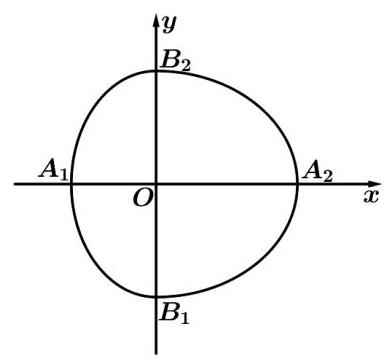
\includegraphics[max width=0.3\textwidth]{images/bo_d5jm9o77aajc7383vmi0_7_1069_1290_388_363_0.jpg}
\end{center}
\hspace*{3em} 

【练习】9. (2025 届大同) 如图,半椭圆 \(\frac{{x}^{2}}{{a}^{2}} + \frac{{y}^{2}}{{b}^{2}} = 1\left( {x \geq  0}\right)\) 与半椭圆 \(\frac{{y}^{2}}{{b}^{2}} + \frac{{x}^{2}}{{c}^{2}} = 1\left( {x < 0}\right)\) 组成的曲线称为 “果圆”,其中 \({a}^{2} = {b}^{2} + \; {c}^{2},a > 0,b > c > 0\) . "果圆 "与 \(x\) 轴的交点分别为 \({A}_{1},{A}_{2}\) ,若在 “果圆” y 轴右侧部分上存在点 \(P\) ，使得 \(\angle {A}_{1}P{A}_{2} = \frac{\pi }{2}\) ，则 \(\frac{c}{a}\) 的取值范围为\_\_\_\_\_.

【答案】 \(\left( {\frac{1}{2},\frac{\sqrt{5} - 1}{2}}\right)\)

【解析】设 \(P\left( {a\cos \theta ,b\sin \theta }\right) ,\cos \theta  \in  \left( {0,1}\right)\) ,

\(\overrightarrow{{A}_{1}P} = \left( {a\cos \theta  + c,b\sin \theta }\right) ,\overrightarrow{{A}_{2}P} = \left( {a\cos \theta  - a,b\sin \theta }\right) ,\)

因为 \(\angle {A}_{1}P{A}_{2} = {90}^{ \circ  }\) ,所以 \(\overrightarrow{{A}_{1}P} \cdot  \overrightarrow{{A}_{2}P} = 0\) ,

所以 \(\left( {a\cos \theta  + c}\right) \left( {a\cos \theta  - a}\right)  + {b}^{2}{\sin }^{2}\theta  = 0\) ,令 \(\frac{c}{a} = t\) ,则 \(\cos \theta  = \frac{1}{{t}^{2}} - \frac{1}{t} - 1\) ,

因为 \(\cos \theta  \in  \left( {0,1}\right)\) ,所以 \(0 < 1 - t - {t}^{2} < {t}^{2}\) ,解得 \(\frac{1}{2} < t < \frac{\sqrt{5} - 1}{2}\) ,

所以 \(\frac{c}{a}\) 的取值范围为 \(\left( {\frac{1}{2},\frac{\sqrt{5} - 1}{2}}\right)\) .

【练习】10. (2024 交附)已知定圆 \(M : {x}^{2} + {y}^{2} = 1\) ，点 \(A\) 是圆 \(M\) 所在平面内一定点，点 \(P\) 是圆 \(M\) 上的动点,若线段 \({PA}\) 的中垂线交直线 \({PM}\) 于点 \(Q\) ,则点 \(Q\) 的轨迹可能是: 2025 版上海高考真题及模拟训练合集(下册)

(1)椭圆；(2)双曲线；(3)抛物线；(4)圆；(5)直线；(6)一个点. 其中所有可能的结果有 ( )

A. 2 个 B. 3 个 C. 4 个 D. 5 个

【答案】 \(C\)

【解析】(1)椭圆 (点 \(A\) 在圆 \(M\) 内,不包括圆心),如图:

因为 \(\left| {AQ}\right|  = \left| {PQ}\right|\) ,所以 \(\left| {AQ}\right|  + \left| {MQ}\right|  = \left| {PQ}\right|  + \left| {MQ}\right|  = \left| {MP}\right|  = 1\) ,

即 \(Q\) 点的轨迹是以 \(A,M\) 为焦点的椭圆；

(2)双曲线(点 \(A\) 在圆 \(M\) 外)，如图:

因为 \(\left| {AQ}\right|  = \left| {PQ}\right|\) ,所以 \(\left| {MQ}\right|  - \left| {AQ}\right|  = \left| {MQ}\right|  - \left| {PQ}\right|  = \left| {MP}\right|  = 1\) ,

即 \(Q\) 点的轨迹是以 \(A,M\) 为焦点的双曲线;

(4)圆(点 \(A\) 恰为圆心)

当 \(A\) 与 \(M\) 重合时, \(Q\) 在 \({MP}\) 中点,

所以 \(Q\) 点的轨迹是以 \(M\) 为圆心,半径为 \(\frac{1}{2}\) 的圆.

(6)一个点 (点 \(A\) 在圆 \(M\) 上)

当 \(A\) 在圆上时, \({AP}\) 为弦,所以 \(Q\) 一定与 \(M\) 重合,所以 \(Q\) 点的轨迹是点 \(M\) .

故选 \(C\) .

\begin{center}
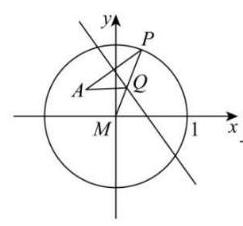
\includegraphics[max width=0.2\textwidth]{images/bo_d5jm9o77aajc7383vmi0_8_306_1010_243_226_0.jpg}
\end{center}
\hspace*{3em} 

yA KO ум

\(M\left( Q\right)\)

\(M \; x\)

\(M \; x\)

【练习】11. 定义:若抛物线的顶点，抛物线与 \(x\) 轴的两个交点构成的三角形是直角三角形，则这种抛物线就称为: “美丽抛物线”. 如图，直线 \(l : y = \frac{1}{3}x + b\) 经过点 \(M\left( {0,\frac{1}{4}}\right)\) ，一组抛物线的顶点 \({B}_{1}\left( {1,{y}_{1}}\right) ,{B}_{2}\left( {2,{y}_{2}}\right) ,{B}_{3}\left( {3,{y}_{3}}\right) ,\cdots ,{B}_{n}\left( {n,{y}_{n}}\right) \left( {n\text{ 为正整数 }}\right)\) ,依次是直线 \(l\) 上的点,这组抛物线与 \(x\) 轴正半轴的交点依次是: \({A}_{1}\left( {{x}_{1},0}\right) ,{A}_{2}\left( {{x}_{2},0}\right) {A}_{3}\left( {{x}_{3},0}\right) ,\cdots ,{A}_{n + 1}\left( {{x}_{n + 1},0}\right) \left( {n\text{ 为正整数 }}\right)\) . 若 \({x}_{1} \; = d\left( {0 < d < 1}\right)\) ,当 \(d\) 为 ( ) 时,这组抛物线中存在美丽抛物线.

\begin{center}
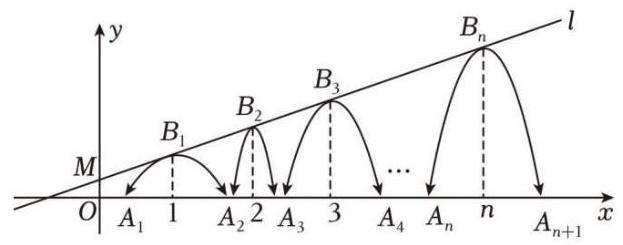
\includegraphics[max width=0.5\textwidth]{images/bo_d5jm9o77aajc7383vmi0_8_287_1523_623_245_0.jpg}
\end{center}
\hspace*{3em} 

A. \(\frac{5}{12}\) 或 \(\frac{7}{12}\) B. \(\frac{5}{12}\) 或 \(\frac{11}{12}\) C. \(\frac{7}{12}\) 或 \(\frac{11}{12}\) D. \(\frac{7}{12}\)

【答案】 \(B\)

【解析】直线 \(l : y = \frac{1}{3}x + b\) 经过点 \(M\left( {0,\frac{1}{4}}\right)\) ,则 \(b = \frac{1}{4}\) ,所以直线 \(l : y = \frac{1}{3}x + \frac{1}{4}\) . 由抛物线的对称性得抛物线的顶点与 \(x\) 轴的两个交点构成的直角三角形必为等腰直角三角形，所以该等腰三角形的高等于斜边的一半. 因为 \(0 < d < 1\) ，所以该等腰直角三角形的斜边长小于 2 ，

斜边上的高小于 1 (即抛物线的顶点纵坐标小于 1 );

因为当 \(x = 1\) 时, \({y}_{1} = \frac{1}{3} \times  1 + \frac{1}{4} = \frac{7}{12} < 1\) ,当 \(x = 2\) 时, \({y}_{2} = \frac{1}{3} \times  2 + \frac{1}{4} = \frac{11}{12} < 1\) ,

当 \(x = 3\) 时, \({y}_{3} = \frac{1}{3} \times  3 + \frac{1}{4} = \frac{5}{4} > 1\) ,所以美丽抛物线的顶点只有 \({B}_{1}{B}_{2}\) .

 \circled{1} 若 \({B}_{1}\) 为顶点，由 \({B}_{1}\left( {1,\frac{7}{12}}\right)\) ，则 \(d = 1 - \frac{7}{12} = \frac{5}{12}\) ；

 \circled{2} 若 \({B}_{2}\) 为顶点，由 \({B}_{2}\left( {2,\frac{11}{12}}\right)\) ，则 \(d = 1 - \left\lbrack  {\left( {2 - \frac{11}{12}}\right)  - 1}\right\rbrack   = \frac{11}{12}\) ，

综上所述， \(d\) 的值为 \(\frac{5}{12}\) 或 \(\frac{11}{12}\) 时，存在美丽抛物线. 故选 \(B\) .

\section*{板块二:压轴客观题}

\section*{1. 真题回顾}

【例题】1. (2023 上海秋考) 在平面上,若曲线 \(\Gamma\) 具有如下性质: 存在点 \(M\) ,使得对于任意点 \(P \in  \Gamma\) ,都有 \(Q \in  \Gamma\) 使得 \(\left| {PM}\right|  \cdot  \left| {QM}\right|  = 1\) ,则称这条曲线为 “自相关曲线”.

关于以下两个结论,正确的判断是 ( )

 \circled{1} 所有椭圆都为“自相关曲线”;  \circled{2} 存在是“自相关曲线”的双曲线.

A.  \circled{1} 成立， \circled{2} 成立 B.  \circled{1} 成立， \circled{2} 不成立

C.  \circled{1} 不成立， \circled{2} 成立 D.  \circled{1} 不成立， \circled{2} 不成立

【答案】 \(B\)

【解析】对于 \circled{1} ,因为椭圆是封闭图形,对于平面上 \(x\) 轴一点 \(M\left( {x,0}\right)\) ,

则其到椭圆 \(\Gamma\) 的最大距离为 \({MP} = x + a\) ,到椭圆 \(\Gamma\) 的最小距离为 \({MQ} = x - a\) ,

若满足 \(\left| {PM}\right|  \cdot  \left| {QM}\right|  = \left( {x + a}\right) \left( {x - a}\right)  = 1 \Rightarrow  {x}^{2} = {a}^{2} + 1 \Rightarrow  x = \sqrt{{a}^{2} + 1}\) ,满足题意,

故 \circled{1} 为真命题；其他位置类似验证；

对于 \circled{2} ，若 \(\Gamma\) 为双曲线，对于任意点 \(P \in  \Gamma\) ， \(\left| {PM}\right|\) 为最大值，

但 \(\left| {PM}\right|  \rightarrow   + \infty\) 无最大值,而 \(\left| {QM}\right|\) 为定长,所以无法满足对任意的 \(P \in  \Gamma\) ,

都存在 \(Q \in  \Gamma\) ,使得 \(\left| {PM}\right|  \cdot  \left| {QM}\right|  = 1\) ,故 \circled{2} 为假命题,

故选 B.

【例题】2. (2022 上海秋考) 已知平面直角坐标系中的点集 \(Q = \left\{  {\left( {x,y}\right) \left| {{\left( x - k\right) }^{2} + {\left( y - {k}^{2}\right) }^{2} = 4}\right| k \mid  ,k \in  }\right. \; \left. Z\right\}\) .

 \circled{1}  存在直线 \(l\) 与 \(Q\) 没有公共点，且 \(Q\) 中存在两点在 \(l\) 的两侧；

 \circled{2} 存在直线 \(l\) 经过 \(Q\) 中的无数个点. 则 ( )

A.  \circled{1} 成立 \circled{2} 成立 B.  \circled{1} 成立 \circled{2} 不成立

C.  \circled{1} 不成立 \circled{2} 成立 D.  \circled{1} 不成立 \circled{2} 不成立

【答案】 \(B\)

\begin{center}
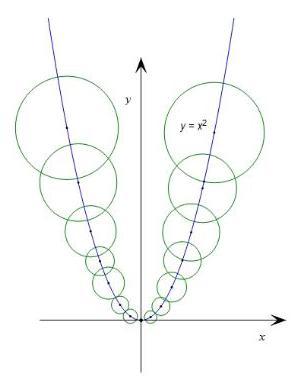
\includegraphics[max width=0.2\textwidth]{images/bo_d5jm9o77aajc7383vmi0_10_1140_1407_291_378_0.jpg}
\end{center}
\hspace*{3em} 

【解析】命题 \circled{1} 成立，理由如下:

由于圆的分布是关于 \(y\) 轴对称，所以考虑 \(y\) 轴右侧的情况，

设第 \(k\) 个圆的半径为 \({r}_{k} = 2\sqrt{k}\) ,

第 \(k + 1\) 个圆的半径为 \({r}_{k + 1} = 2\sqrt{k + 1}\) ,

我们很想有一条水平可以将这一堆圆无交集地隔开,

这等价于了两圆的半径之和是否小于圆心纵坐标的差.

即 \(\Delta {y}_{k} = {y}_{k + 1} - {y}_{k} = {\left( k + 1\right) }^{2} - {k}^{2} = {2k} + 1\) ,

法一:利用极限 \(\mathop{\lim }\limits_{{k \rightarrow  \infty }}\frac{\Delta {y}_{k}}{{r}_{k} + {r}_{k + 1}} = \frac{{2k} + 1}{2\sqrt{k} + 2\sqrt{k + 1}} \rightarrow   + \infty\) ，

由极限定义得存在 \(K\) ，当 \(k > K\) 时，有上下四个圆均可存在一条水平线满足条件.

法二: 因为 \(\Delta {y}_{k} = {2k} + 1\) 是一条直线,

\({r}_{k} + {r}_{k + 1} = 2\sqrt{k} + 2\sqrt{k + 1}\) 呈现出类似 \(y = \sqrt{x}\) 的增长形式,故必有足够大的 \(K\) ,

当 \(k > K\) 时,有 \(\Delta {y}_{k} > {r}_{k} + {r}_{k + 1}\) .

所以存在一条水平可以将这一堆圆无交集地隔开,

命题 \circled{2} 不成立，理由如下:

由于圆的分布的对称性,我们同样考虑 \(y\) 轴右侧的情况,

假设直线为 \({ax} + {by} + c = 0\) ,则圆心到点的距离为 \({D}_{k} = \frac{\left| ak + b{k}^{2} + c\right| }{\sqrt{{a}^{2} + {b}^{2}}}\) ,

又因为半径为 \({r}_{k} = 2\sqrt{k}\) ,

法一:利用极限 \(\mathop{\lim }\limits_{{k \rightarrow  \infty }}\frac{{D}_{k}}{{r}_{k}} = \mathop{\lim }\limits_{{k \rightarrow  \infty }}\frac{\frac{{ak} + b{k}^{2} + c}{\sqrt{{a}^{2} + {b}^{2}}}}{2\sqrt{k}} = \mathop{\lim }\limits_{{k \rightarrow  \infty }}\frac{\left| ak + b{k}^{2} + c\right| }{2\sqrt{k} \cdot  \sqrt{{a}^{2} + {b}^{2}}} \rightarrow   + \infty\) ,

故存在 \(K\) ,当 \(k > K\) 时有直线与圆相离.

因为 \(y\) 右侧与直线有交集的圆的个数是有限的,

同理可知左侧满足条件的圆也是有限的.

左侧情况画图观察也是很显然的.

法二: \({D}_{k} = \frac{\left| ak + b{k}^{2} + c\right| }{\sqrt{{a}^{2} + {b}^{2}}}\) 是一个二次函数或中间有一段翻折上来的一部分,

\({D}_{k} = f\left( k\right)\) 是下凸函数的一部分,而 \({r}_{k} = 2\sqrt{k}\) 是上凸函数,

必然存在足够大的 \(K\) ,当 \(k > K\) 时, \({D}_{k} > {r}_{k}\) ,

故选 \(B\) .

【例题】3. (2017 上海秋考) 如图,用 35 个单位正方形拼成一个矩形,点 \({P}_{1}\) 、 \({P}_{2}\text{ 、 }{P}_{3}\text{ 、 }{P}_{4}\) 以及四个标记为“ \(\bigtriangleup\) ”的点在正方形的顶点处,设集合 \(\Omega  = \; \left\{  {{P}_{1},{P}_{2},{P}_{3},{P}_{4}}\right\}\) ,点 \(P \in  \Omega\) ,过 \(P\) 作直线 \({l}_{P}\) ,使得不在 \({l}_{P}\) 上的 “ \(\bigtriangleup\) ” 的点分布在 \({l}_{P}\) 的两侧. 用 \({D}_{1}\left( {l}_{P}\right)\) 和 \({D}_{2}\left( {l}_{P}\right)\) 分别表示 \({l}_{P}\) 一侧和另一侧的“ \(\Delta\) ” 的点到 \({l}_{P}\) 的距离之和. 若过 \(P\) 的直线 \({l}_{P}\) 中有且只有一条满足 \({D}_{1}\left( {l}_{P}\right) \; = {D}_{2}\left( {l}_{P}\right)\) ,则 \(\Omega\) 中所有这样的 \(P\) 为\_\_\_\_\_.

\begin{center}
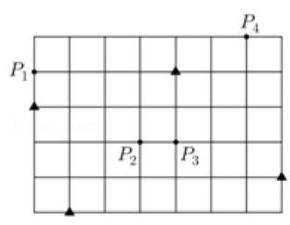
\includegraphics[max width=0.2\textwidth]{images/bo_d5jm9o77aajc7383vmi0_11_1163_950_290_225_0.jpg}
\end{center}
\hspace*{3em} 

【答案】 \({P}_{1}\text{ 、 }{P}_{3}\text{ 、 }{P}_{4}\)

【解析】法一:建立平面直角坐标系,如图所示;

则记为“ \(\bigtriangleup\) ”的四个点是 \(A\left( {0,3}\right) ,B\left( {1,0}\right) ,C\left( {7,1}\right) ,D\left( {4,4}\right)\) ,

线段 \({AB}\text{ 、 }{BC}\text{ 、 }{CD}\text{ 、 }{DA}\) 的中点分别为 \(E\text{ 、 }F\text{ 、 }G\text{ 、 }H\) ,

易得 \({EFGH}\) 为平行四边形,如图所示,设四边形重心为 \(M\left( {x,y}\right)\) ,

则 \(\overrightarrow{MA} + \overrightarrow{MB} + \overrightarrow{MC} + \overrightarrow{MD} = \overrightarrow{0}\) ,由此求得 \(M\left( {3,2}\right)\) ,

即平行四边形 \({EFGH}\) 的对角线交于点 \({P}_{2}\) ,则符合条件的直线 \({l}_{P}\) 一定经过点 \({P}_{2}\) ,

\begin{center}
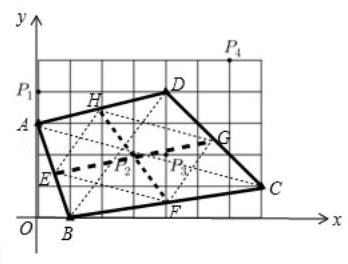
\includegraphics[max width=0.2\textwidth]{images/bo_d5jm9o77aajc7383vmi0_11_1102_1529_348_264_0.jpg}
\end{center}
\hspace*{3em} 

且过点 \({P}_{2}\) 的直线有无数条;

由过点 \({P}_{1}\) 和 \({P}_{2}\) 的直线有且仅有 1 条,过点 \({P}_{3}\) 和 \({P}_{2}\) 的直线有且仅有 1 条,

过点 \({P}_{4}\) 和 \({P}_{2}\) 的直线有且仅有 1 条,所以符合条件的点是 \({P}_{1}\text{ 、 }{P}_{3}\) 、 \({P}_{4}\) .

法二:建立适当的直角坐标系,四个\#的坐标为 \(\left( {1,0}\right) ,\left( {7,1}\right) ,(0\)

3), \(\left( {4,4}\right)\) ,

\({P}_{1}\left( {0,4}\right) ,{P}_{2}\left( {3,2}\right) ,{P}_{3}\left( {4,2}\right) ,{P}_{4}\left( {6,5}\right) ,\)

设 \({l}_{P}\) 直线方程为 \({ax} + {by} + c = 0\) ,由 \({D}_{1}\left( {l}_{P}\right)  = {D}_{2}\left( {l}_{P}\right)\) 得四个 \(\#\) 到直线 \({l}_{P}\) 的有向距离

之和为 0,则 \(\frac{a + c}{\sqrt{{a}^{2} + {b}^{2}}} + \frac{{7a} + b + c}{\sqrt{{a}^{2} + {b}^{2}}} + \frac{{3b} + c}{\sqrt{{a}^{2} + {b}^{2}}} + \frac{{4a} + {4b} + c}{\sqrt{{a}^{2} + {b}^{2}}} = 0\) ,

得 \({12a} + {8b} + {4c} = 0\) ,所以 \({3a} + {2b} + c = 0\) ,即 \({ax} + {by} + c = 0\) 过点 \(\left( {3,2}\right)\) ,

\({l}_{P}\) 过点 \({P}_{2}\) 就能满足 \({D}_{1}\left( {l}_{P}\right)  = {D}_{2}\left( {l}_{P}\right)\) ,

又因为过 \(P\) 的直线 \({l}_{P}\) 中有且只有一条,所以 \({l}_{P}\) 还要过 \({P}_{1},{P}_{3},{P}_{4}\) 任何一点都能唯一, 所以符合条件的点是 \({P}_{1}\text{ 、 }{P}_{3}\text{ 、 }{P}_{4}\) .

【例题】4. (2019 上海春考) 在椭圆 \(\frac{{x}^{2}}{4} + \frac{{y}^{2}}{2} = 1\) 上任意一点 \(P,Q\) 与 \(P\) 关于 \(x\) 轴对称,若有 \(\overrightarrow{{F}_{1}P} \cdot  \overrightarrow{{F}_{2}P} \leq\) 1,则 \(\overrightarrow{{F}_{1}P}\) 与 \(\overrightarrow{{F}_{2}Q}\) 的夹角范围为\_\_\_\_\_.

【答案】 \(\left\lbrack  {\pi  - \arccos \frac{1}{3},\pi }\right\rbrack\)

【解析】设 \(P\left( {x,y}\right)\) ,则 \(Q\) 点 \(\left( {x, - y}\right)\) ,椭圆 \(\frac{{x}^{2}}{4} + \frac{{y}^{2}}{2} = 1\) 的焦点坐标为 \(\left( {-\sqrt{2},0}\right) \text{ 、 }\left( {\sqrt{2},0}\right)\) ,

因为 \(\overrightarrow{{F}_{1}P} \cdot  \overrightarrow{{F}_{2}P} \leq  1\) ,所以 \({x}^{2} - 2 + {y}^{2} \leq  1\) ,结合 \(\frac{{x}^{2}}{4} + \frac{{y}^{2}}{2} = 1\) ,得 \({y}^{2} \in  \left\lbrack  {1,2}\right\rbrack\) ,

故 \(\overrightarrow{{F}_{1}P}\) 与 \(\overrightarrow{{F}_{2}Q}\) 的夹角 \(\theta\) 满足 \(\cos \theta  = \frac{\overrightarrow{{F}_{1}P} \cdot  \overrightarrow{{F}_{2}Q}}{\left| \overrightarrow{{F}_{1}P}\right|  \cdot  \left| \overrightarrow{{F}_{2}Q}\right| } = \frac{{x}^{2} - 2 - {y}^{2}}{\sqrt{{\left( {x}^{2} + 2 + {y}^{2}\right) }^{2} - 8{x}^{2}}}\)

\(= \frac{2 - 3{y}^{2}}{{y}^{2} + 2} =  - 3 + \frac{8}{{y}^{2} + 2} \in  \left\lbrack  {-1, - \frac{1}{3}}\right\rbrack\) ,故 \(\theta  \in  \left\lbrack  {\pi  - \arccos \frac{1}{3},\pi }\right\rbrack\) .

【例题】5. (2017 上海秋考) 在平面直角坐标系 \({xOy}\) 中,已知椭圆 \({C}_{1} : \frac{{x}^{2}}{36} + \frac{{y}^{2}}{4} = 1\) 和 \({C}_{2} : {x}^{2} + \frac{{y}^{2}}{9} = 1\) . \(P\) 为 \({C}_{1}\) 上的动点, \(Q\) 为 \({C}_{2}\) 上的动点, \(w\) 是 \(\overrightarrow{OP} \cdot  \overrightarrow{OQ}\) 的最大值. 记 \(\Omega  = \{ \left( {P,Q}\right)  \mid  P\) 在 \({C}_{1}\) 上, \(Q\) 在 \({C}_{2}\) 上,且 \(\overrightarrow{OP} \cdot  \overrightarrow{OQ} = w\}\) ,则 \(\Omega\) 中元素个数为 ( )

A. 2 个 B. 4 个 C. 8 个 D. 无穷个

【答案】 \(D\)

【解析】椭圆 \({C}_{1} : \frac{{x}^{2}}{36} + \frac{{y}^{2}}{4} = 1\) 和 \({C}_{2} : {x}^{2} + \frac{{y}^{2}}{9} = 1.P\) 为 \({C}_{1}\) 上的动点, \(Q\) 为 \({C}_{2}\) 上的动点,

法一: 设 \(P\left( {6\cos \alpha ,2\sin \alpha }\right) ,Q\left( {\cos \beta ,3\sin \beta }\right) ,0 \leq  \alpha \text{ 、 }\beta  < {2\pi }\) ,

则 \(\overrightarrow{OP} \cdot  \overrightarrow{OQ} = 6\cos \alpha \cos \beta  + 6\sin \alpha \sin \beta  = 6\cos \left( {\alpha  - \beta }\right)\) ,

当 \(\alpha  = \beta\) 时， \(w\) 取得最大值 6 ，

则 \(\Omega  = \{ \left( {P,Q}\right)  \mid  P\) 在 \({C}_{1}\) 上， \(Q\) 在 \({C}_{2}\) 上，且 \(\overrightarrow{OP} \cdot  \overrightarrow{OQ} = w\}\) 中的元素有无穷多对.

法二: 令 \(P\left( {m,n}\right) ,Q\left( {u,v}\right)\) ,则 \({m}^{2} + 9{n}^{2} = {36},9{u}^{2} + {v}^{2} = 9\) ,

由柯西不等式得 \(\left( {{m}^{2} + 9{n}^{2}}\right) \left( {9{u}^{2} + {v}^{2}}\right)  = {324} \geq  {\left( 3mu + 3nv\right) }^{2}\) ,

当且仅当 \({mv} = {9nu}\) ,取得最大值 6 ,

显然,满足条件的 \(P\text{ 、 }Q\) 有无穷多对, \(D\) 项正确.

故选 \(D\) .

\section*{2. 模拟练习}

【练习】1. (2024 届华二)已知 \(P,Q\) 是曲线 \(\Gamma\) 上两点，若存在 \(M\) 点，使得曲线 \(\Gamma\) 上任意一点 \(P\) 都存在 \(Q\) 使得 \(\overrightarrow{MP} \cdot  \overrightarrow{MQ} = 1\) ，则称曲线 \(\Gamma\) 是 “自相关曲线”，现有如下两个命题: \circled{1} 存在双曲线是 “自相关曲线”;  \circled{2}  任意椭圆都是 “自相关曲线”，则 ( )

A.  \circled{1} 成立， \circled{2} 成立 B.  \circled{1} 成立， \circled{2} 不成立

C.  \circled{1} 不成立， \circled{2} 成立 D.  \circled{1} 不成立， \circled{2} 不成立

【答案】 \(A\)

【解析】法一:对 \circled{1} ，考虑双曲线 \(y = \frac{1}{3x}\) ，并令 \(M\) 为坐标原点，则对任意 \(P\left( {t,\frac{1}{3t}}\right)\) ，

都存在 \(Q\left( {\frac{3 + \sqrt{5}}{6t},\frac{3 - \sqrt{5}}{2}t}\right)\) ,使得 \(\overrightarrow{MP} \cdot  \overrightarrow{MQ} = 1\) . 因此 \circled{1} 正确.

对 \circled{2} ，设椭圆方程为 \(\frac{{x}^{2}}{{a}^{2}} + \frac{{y}^{2}}{{b}^{2}} = 1\left( {a > b > 0}\right)\) ，令 \(M\left( {m,0}\right)\) ，其中 \(m =  - \sqrt{{a}^{2} + 1}\) .

对椭圆上的任意点 \(P\) ，设 \(P\left( {a\cos \alpha ,b\sin \alpha }\right)\) .

则只需验证关于 \(\theta\) 的方程 \(\left( {a\cos \theta  - m}\right) \left( {a\cos \alpha  - m}\right)  + {b}^{2}\sin \theta \sin \alpha  = 1\left( *\right)\)

在区间 \(\lbrack 0,{2\pi })\) 上有异于 \(\alpha\) 的解.

当 \(\alpha  = 0\) 或 \(\pi\) 时可相应地取 \(\theta  = \pi\) 或 0 .

下设 \(\alpha  \notin  \{ 0,\pi \}\) .

则 (*) 等价于 \(a\left( {a\cos \alpha  - m}\right) \cos \theta  + {b}^{2}\sin \alpha \sin \theta  = m\left( {a\cos \alpha  - m}\right)  + 1\) ,

故当 \({a}^{2}{\left( a\cos \alpha  - m\right) }^{2} + {b}^{4}{\sin }^{2}\alpha  > {\left\lbrack  m\left( a\cos \alpha  - m\right)  + 1\right\rbrack  }^{2}\) 时 (*) 必有解.

移项重新配方,利用 \({m}^{2} = {a}^{2} + 1\) ,

上式等价 \({b}^{4}{\sin }^{2}a + {a}^{2} > {\left\lbrack  \left( a\cos \alpha  - m\right)  + m\right\rbrack  }^{2} = {a}^{2}{\cos }^{2}\alpha\) .

当 \(\alpha  \notin  \{ 0,\pi \}\) 时该式成立，故 (*) 必有解，

同时，上述不等关系表明此时的(*)在区间 \(\lbrack 0,{2\pi })\) 上有两个不同的解，

因此必能找到 (*) 在 \(\lbrack 0,{2\pi })\) 上有异于 \(\alpha\) 的解，因此 \circled{2} 正确；

故选 \(A\) .

法二:对 \circled{1} :对于双曲线，取 \(M\) 为 \(x\) 轴正半轴的充分靠右的点，

则 \(\left| {MP}\right|\) 的最小值充分大，由数量积投影，

经过 \(M\) 附近的点的直线一定与双曲线有交点，所以任意双曲线都是“自相关曲线”；

对 \circled{2} :设 \(M\) 在 \(x\) 轴正半轴，设长轴顶点为 \(A,B\) ，则猜测 \({MA},{MB}\) 必须配对，

所以有 \({MA} \cdot  {MB} = 1\) ,此时任取 \(P\) ,则 \(\overrightarrow{MP}\) 在 \(x\) 轴投影介于 \(\left\lbrack  {{MA},{MB}}\right\rbrack\) 之间,

所以 \(\overrightarrow{MP} \cdot  \overrightarrow{MA} \leq  {MA} \cdot  {MB} = 1\) ,而 \(\overrightarrow{MP} \cdot  \overrightarrow{MB} \geq  {MA} \cdot  {MB} = 1\) ,

由连续性和零点定理,存在 \(Q\) 满足要求;

故选 \(A\) .

【练习】2. (2026 复附期中) 已知曲线 \(\Gamma\) 的对称中心为 \(O\) ,如果对于曲线 \(\Gamma\) 上的任意一点 \(A\) ,都存在 \(\Gamma\) 上另外的两点 \(B,C\) ,使得 \(\bigtriangleup {ABC}\) 的垂心为 \(O\) ,则称 \(\Gamma\) 为“自垂曲线”. 现有如下两个命题:

 \circled{1} 任意双曲线都是“自垂曲线”;  \circled{2} 任意椭圆都是“自垂曲线”.

则下列判断正确的是( ).

A.  \circled{1} 是真命题， \circled{2} 是真命题 B.  \circled{1} 是假命题， \circled{2} 是真命题

C.  \circled{1} 是真命题， \circled{2} 是假命题 D.  \circled{1} 是假命题， \circled{2} 是假命题

【答案】 \(B\)

【解析】 \circled{1}  错误,解法 1: 假设双曲线 \(\Gamma  : \frac{{x}^{2}}{{a}^{2}} - \frac{{y}^{2}}{{b}^{2}} = 1\left( {b > a > 0}\right)\) 上存在一点 \(A\) ,且 \({k}_{OA} = \frac{a}{b}\) . 根据 \(b > \; a \Rightarrow  {k}_{OA} = \frac{a}{b} < \frac{b}{a}\) ,即 \(A\) 点为 \(y = \frac{a}{b}x\) 和双曲线在第一象限的交点,所以此时 \({k}_{BC} =  - \frac{b}{a}\) ,这样的 \({l}_{BC}\) 与双曲线只有一个交点,所以存在双曲线不是 “自垂曲线.”

所以 \circled{1} 错误.

解法 2: 取 \(A\left( {1,1}\right) ,B\left( {{x}_{0},\frac{1}{{x}_{0}}}\right) ,C\left( {\frac{1}{{x}_{0}},{x}_{0}}\right)\) .

\(\because {k}_{OB} \cdot  {k}_{AC} =  - 1 \Rightarrow  \frac{\frac{1}{{x}_{0}}}{{x}_{0}} \cdot  \frac{1 - {x}_{0}}{1 - \frac{1}{{x}_{0}}} =  - 1 \Rightarrow  \frac{1}{{x}_{0}} - 1 = 1 - {x}_{0} \Rightarrow  {x}_{0} = 1\) 与点 \(A\) 重合矛盾.

\begin{center}
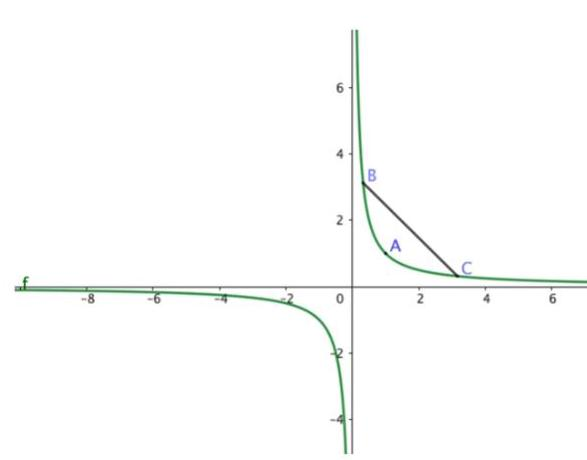
\includegraphics[max width=0.5\textwidth]{images/bo_d5jm9o77aajc7383vmi0_14_286_685_587_460_0.jpg}
\end{center}
\hspace*{3em} 

\begin{center}
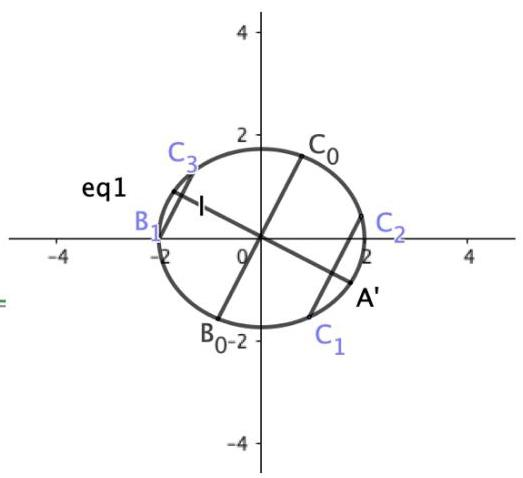
\includegraphics[max width=0.4\textwidth]{images/bo_d5jm9o77aajc7383vmi0_14_879_666_523_478_0.jpg}
\end{center}
\hspace*{3em} 

 \circled{2} 正确:首先任意取一点 \(A\) ，找到 \({B}_{0}{C}_{0}\bot {OA}\) ，作 \({B}_{1}{C}_{1}//{B}_{0}{C}_{0},{B}_{2}{C}_{2}//{B}_{0}{C}_{0}\) ，当 \({B}_{0}{C}_{0} \rightarrow  {B}_{1}{C}_{1}\) 时， 点 \({C}_{1}\) 趋向于点 \(A\) ，此时 \(\left\langle  {\overrightarrow{O{B}_{1}},\overrightarrow{A{C}_{1}}}\right\rangle\) 极限为钝角，同理当 \({B}_{0}{C}_{0} \rightarrow  {B}_{2}{C}_{2}\) 时， \({B}_{1}\) 趋向于点 \({A}^{\prime }\) ，此时 \(\left\langle  {\overrightarrow{O{B}_{2}},\overrightarrow{A{C}_{2}}}\right\rangle\) 为锐角，所以在这两种位置之间存在直角的情况，所以 \circled{2} 正确.

【练习】3. 若恰有三组不全为 0 的实数对 \(\left( {a\text{ 、 }b}\right)\) 满足关系式 \(\left| {a + b + 1}\right|  = \left| {{4a} - {3b} + 1}\right|  = t\sqrt{{a}^{2} + {b}^{2}}\) ,则实数 \(t\) 的所有可能的值组成的集合为\_\_\_\_\_.

【答案】 \(\left\{  {\frac{5}{2},\frac{7}{5},\frac{7\sqrt{29}}{29}}\right\}\)

【解析】由已知得 \(t > 0\) ,整理得 \(\frac{\left| a + b + 1\right| }{\sqrt{{a}^{2} + {b}^{2}}} = \frac{\left| 4a - 3b + 1\right| }{\sqrt{{a}^{2} + {b}^{2}}} = t\) ,

看成有且仅有三条直线满足 \(A\left( {1,1}\right)\) 和 \(B\left( {4, - 3}\right)\) 到直线 \({ax} + {by} + c = 0\) 不过原点) 的距离 \(t\) 相等.

由 \(\left| {AB}\right|  = \sqrt{{\left( 4 - 1\right) }^{2} + {\left( -3 - 1\right) }^{2}} = 5\) ,

(1)当 \(t = \frac{\left| AB\right| }{2} = \frac{5}{2}\) ，此时易得符合题意的直线 \(l\) 为线段 \({AB}\) 的垂直平分线 \({6x} - {8y} - {23} = 0\) 以及直线 \({AB}\) 平行的两条直线 \({8x} + {6y} + {11} = 0\) 和 \({8x} + {6y} - {39} = 0\) ;

( 2 )当 \(t < \frac{\left| AB\right| }{2} = \frac{5}{2}\) 时，有 4 条直线 \(l\) 会使得点 \(A\left( {1,1}\right)\) 和 \(B\left( {4, - 3}\right)\) 到它们的距离相等,注意到 \(l\) 不过原点，

所以当其中一条直线过原点时,会作为增根被舍去.

设点 \(A\) 到 \(l\) 的距离为 \(d\) ,

 \circled{1} 作为增根被舍去的直线 \(l\) ，过原点和 \(A,B\) 的中点 \(M\left( {\frac{5}{2}, - 1}\right)\) ，其方程为 \({2x} + {5y} = 0\) ，此时 \(t\)

\(= d = \frac{7}{\sqrt{29}} < \frac{5}{2}\) ,符合;

 \circled{2} 作为增根被舍去的直线 \(l\) ，过原点且以 \(\overrightarrow{AB}\) 为方向向量，其方程为 \({4x} + {3y} = 0\) ，此时， \(t = d = \; \frac{7}{5} < \frac{5}{2}\) ,符合;

综上,满足题意的实数 \(t\) 为 \(\frac{5}{2},\frac{7}{5},\frac{7\sqrt{29}}{29}\) .

故答案为: \(\frac{5}{2},\frac{7}{5},\frac{7\sqrt{29}}{29}\) .

【练习】4. (2024 届华二) 点 \(P\) 为抛物线 \(C : {y}^{2} = {4x}\) 准线上的点,若存在过 \(P\) 的直线交抛物线 \(C\) 于 \(A,B\) 两点,且 \(\left| {PA}\right|  = \left| {AB}\right|\) ,则称点 \(P\) 为“ \(\Omega\) 点”,那么下列结论中正确的是 ( )

A. 准线上的所有点都不是 “ \(\Omega\) 点”

B. 准线上的所有点都是 “ \(\Omega\) 点”

C. 准线上仅有有限个点是 “ \(\Omega\) 点”

D. 准线上有无穷多个点 (不是所有的点) 是 “Ω点”

【答案】 \(B\)

【解析】由题意可知抛物线 \(C : {y}^{2} = {4x}\) 的准线方程为: \(x =  - 1\) .

设 \(A\left( {m,n}\right) ,P\left( {-1,y}\right)\) ,因为 \(\left| {PA}\right|  = \left| {AB}\right|\) ,所以 \(A\) 为 \({PB}\) 中点,则 \(B\left( {{2m} + 1,{2n} - y}\right)\) .

\(\because A,B\) 在 \({y}^{2} = {4x}\) 上, \(\therefore {n}^{2} = {4m}\) 且 \({\left( 2n - y\right) }^{2} = 4\left( {{2m} + 1}\right)\) ,消去 \(m\) 得, \(2{n}^{2} + 4 = {\left( 2n - y\right) }^{2}\) ,

整理得关于 \(n\) 的方程 \(2{n}^{2} - {4yn} + {y}^{2} - 4 = 0,\because \Delta  = 8{y}^{2} + {32} > 0\) 恒成立, \(\therefore\) 该方程恒有实数解.

即对于任意的 \(P\) 点,都存在 \(m\) ,使得 \(\left| {PA}\right|  = \left| {AB}\right|\) ,故选 \(B\) .

【练习】5. 设双曲线的焦点为 \(\left( {\pm c,0}\right)\) ,圆 \(C : {\left( x - c\right) }^{2} + {y}^{2} = {r}^{2}\) ,则 ( )

A. 存在 \(c\) ,使得对任意的 \(r\) ,圆与双曲线至少有一个公共点

B. 存在 \(c\) ,使得对任意的 \(r\) ,圆与双曲线至多有两个公共点

C. 对于任意 \(r\) ，存在 \(c\) ，圆与双曲线至少有两个公共点

D. 对于任意 \(r\) ，存在 \(c\) ，圆与双曲线至多有一个公共点

【答案】 \(C\)

【解析】设双曲线方程为 \(\frac{{x}^{2}}{{a}^{2}} - \frac{{y}^{2}}{{b}^{2}} = 1\) ,与圆方程联立可得: \({c}^{2}{x}^{2} - {2c}{a}^{2}x + {a}^{4} - {a}^{2}{r}^{2} = 0\) ,

解得 \(x = \frac{{a}^{2} \pm  {ar}}{c}\) (以 \(\frac{{a}^{2}}{c}\) 为中点),分类讨论可知:

当 \(\frac{{a}^{2} + {ar}}{c} < a \Rightarrow  a + r < c\) ,无交点;

当 \(\frac{{a}^{2} + {ar}}{c} = a \Rightarrow  a + r = c\) 时,有 1 个交点;

\begin{center}
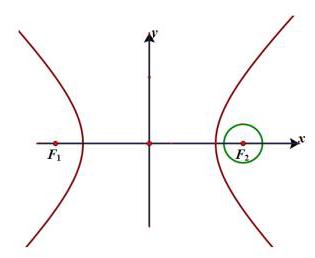
\includegraphics[max width=0.2\textwidth]{images/bo_d5jm9o77aajc7383vmi0_15_307_1792_315_258_0.jpg}
\end{center}
\hspace*{3em} 

\begin{center}
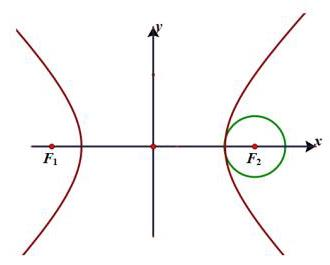
\includegraphics[max width=0.2\textwidth]{images/bo_d5jm9o77aajc7383vmi0_15_647_1776_330_265_0.jpg}
\end{center}
\hspace*{3em} 

当 \(\left\{  {\begin{array}{l} \frac{{a}^{2} - {ar}}{c} >  - a \\  \frac{{a}^{2} + {ar}}{c} > a \end{array} \Rightarrow  c - a < r < c + a}\right.\) 时,有 2 个交点;

当 \(\frac{{a}^{2} - {ar}}{c} =  - a \Rightarrow  r = c + a\) 时,有 3 个交点;

当 \(\frac{{a}^{2} - {ar}}{c} <  - a \Rightarrow  r > c + a\) 时,有 4 个交点;

故对于任意 \(r\) ，存在 \(c\) ，圆与双曲线至少有两个公共点

\begin{center}
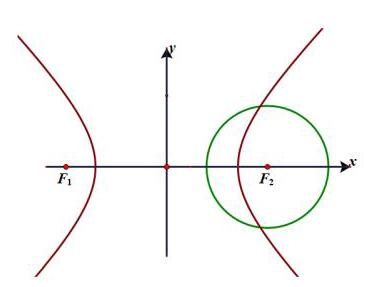
\includegraphics[max width=0.3\textwidth]{images/bo_d5jm9o77aajc7383vmi0_16_308_584_366_287_0.jpg}
\end{center}
\hspace*{3em} 

\begin{center}
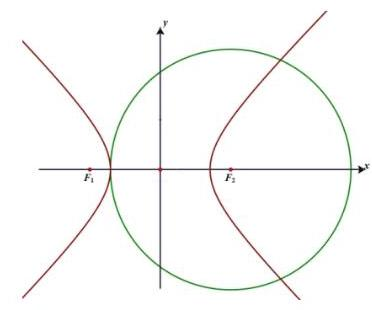
\includegraphics[max width=0.3\textwidth]{images/bo_d5jm9o77aajc7383vmi0_16_696_553_372_310_0.jpg}
\end{center}
\hspace*{3em} 

\begin{center}
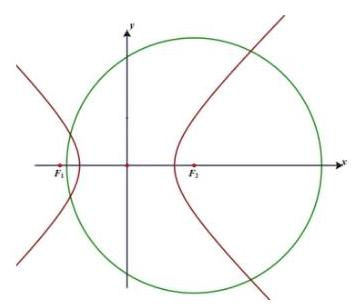
\includegraphics[max width=0.3\textwidth]{images/bo_d5jm9o77aajc7383vmi0_16_1082_553_354_307_0.jpg}
\end{center}
\hspace*{3em} 

【练习】6. 已知 \(P\left( {{x}_{0},{y}_{0}}\right)\) 为圆 \(C : {\left( x - t\right) }^{2} + {\left( y - s\right) }^{2} = {r}^{2}\left( {r > 0}\right)\) 上的任意一点,当 \(a \neq  b\) 时, \(\left| {{x}_{0} - {y}_{0} + a}\right|  + \left| {{x}_{0} - {y}_{0} + b}\right|\) 的值与 \({x}_{0}\text{ 、 }{y}_{0}\) 无关，下列结论正确的是\_\_\_\_\_.

 \circled{1}  当 \(\left| {a - b}\right|  = 2\sqrt{2}r\) 时，点 \(\left( {t,s}\right)\) 的轨迹是一条直线；

 \circled{2}  当 \(\left| {a - b}\right|  = 2\sqrt{2}\) 时，有 \(r\) 的最大值为 1 ；

 \circled{3}  当 \(r = \sqrt{2},b = 2\) 时， \(a\) 的取值范围 \(a \geq  6\) .

【答案】 \circled{1}  \circled{2} 

【解析】 \(P\left( {{x}_{0},{y}_{0}}\right)\) 为圆 \(C : {\left( x - t\right) }^{2} + {\left( y - s\right) }^{2} = {r}^{2}\left( {r > 0}\right)\) 上的任意一点,

当 \(a \neq  b\) 时, \(\left| {{x}_{0} - {y}_{0} + a}\right|  + \left| {{x}_{0} - {y}_{0} + b}\right|\) 的值与 \({x}_{0},{y}_{0}\) 无关,

\(\left| {{x}_{0} - {y}_{0} + a}\right|  + \left| {{x}_{0} - {y}_{0} + b}\right|\) 为圆上的点到两条平行线距离和的 \(\sqrt{2}\) 倍,

则圆在两条平行线 \(x - y + a = 0\) 与 \(x - y + b = 0\) 之间,

\(\left| {a - b}\right|\) 表示两条平行线之间距离的 \(\sqrt{2}\) 倍.

当 \(\left| {a - b}\right|  = 2\sqrt{2}r\) 时,点 \(\left( {t,s}\right)\) 的轨迹是一条直线,

与 \(x - y + a = 0\) 以及 \(x - y + b = 0\) 等距离的直线,所以 \circled{1} 正确.

当 \(\left| {a - b}\right|  = 2\sqrt{2}\) 时,有 \(r\) 的最大值为 1,正确.

当 \(r = \sqrt{2},b = 2\) 时,得 \(\left| {a - 2}\right|  \geq  4\) ,解得 \(a \geq  6\) 或 \(a \leq   - 2\) ,所以 \circled{3} 不正确.

故正确的是 \circled{1}  \circled{2} .

\section*{板块三: 中档主观题}

注:近几年解析几何变成纯 20 题以后就没有了,如果是为了练习 \({20} - 1\) 和 2 可以适当做做,模拟训练就不放了，做压轴模拟训练的前两问更好

\section*{1. 真题回顾}

【例题】1. (2018 上海春考) 已知 \(a \in  R\) ,双曲线 \(\Gamma  : \frac{{x}^{2}}{{a}^{2}} - {y}^{2} = 1\) .

(1)若点 \(\left( {2,1}\right)\) 在 \(\Gamma\) 上，求 \(\Gamma\) 的焦点坐标；

(2)若 \(a = 1\) ，直线 \(y = {kx} + 1\) 与 \(\Gamma\) 相交于 \(A\) 、 \(B\) 两点，且线段 \({AB}\) 中点的横坐标为 1，求实数 \(k\) 的值.

【解析】(1) 把 (2,1) 代入双曲线方程得 \(\frac{4}{{a}^{2}} - 1 = 1\) ,所以 \({a}^{2} = 2\) ,所以 \(c = \sqrt{2 + 1} = \sqrt{3}\) ,

所以 \(\Gamma\) 的焦点坐标为 \(\left( {-\sqrt{3},0}\right) ,\left( {\sqrt{3},0}\right)\) .

(2)当 \(a = 1\) 时，双曲线方程为 \({x}^{2} - {y}^{2} = 1\) ，

由 \(\left\{  \begin{array}{l} {x}^{2} - {y}^{2} = 1 \\  y = {kx} + 1 \end{array}\right.\) ,得 \(\left( {1 - {k}^{2}}\right) {x}^{2} - {2kx} - 2 = 0\) ,

因为直线 \(y = {kx} + 1\) 与 \(\Gamma\) 相交于 \(A\text{ 、 }B\) 两点,所以 \(\bigtriangleup  = 4{k}^{2} + 8\left( {1 - {k}^{2}}\right)  > 0\) ,

解得 \(- \sqrt{2} < k < \sqrt{2}\) . 设 \(A\left( {{x}_{1},{y}_{1}}\right) ,B\left( {{x}_{2},{y}_{2}}\right)\) ,则 \({x}_{1} + {x}_{2} = \frac{2k}{1 - {k}^{2}} = 2\) ,

解得 \(k = \frac{-1 + \sqrt{5}}{2}\) 或 \(k = \frac{-1 - \sqrt{5}}{2}\) (舍). 故 \(k = \frac{-1 + \sqrt{5}}{2}\) .

【例题】2. (2017 上海春考) 已知双曲线 \(\Gamma  : {x}^{2} - \frac{{y}^{2}}{{b}^{2}} = 1\left( {b > 0}\right)\) ,直线 \(l : y = {kx} + m\left( {\mathrm{\;{km}} \neq  0}\right) ,l\) 与 \(\Gamma\) 交于 \(P\text{ 、 }Q\) 两点, \({P}^{\prime }\) 为 \(P\) 关于 \(y\) 轴的对称点,直线 \({P}^{\prime }Q\) 与 \(y\) 轴交于点 \(N\left( {0,n}\right)\) ;

(1)若点 \(\left( {2,0}\right)\) 是 \(\Gamma\) 的一个焦点，求 \(\Gamma\) 的渐近线方程；

(2)若 \(b = 1\) ，点 \(P\) 的坐标为 \(\left( {-1,0}\right)\) ，且 \(\overrightarrow{N{P}^{\prime }} = \frac{3}{2}\overrightarrow{{P}^{\prime }Q}\) ，求 \(k\) 的值；

(3) 若 \(m = 2\) ，求 \(n\) 关于 \(b\) 的表达式.

【解析】(1) 因为双曲线 \(\Gamma  : {x}^{2} - \frac{{y}^{2}}{{b}^{2}} = 1\left( {b > 0}\right)\) ,点 \(\left( {2,0}\right)\) 是 \(\Gamma\) 的一个焦点,

所以 \(c = 2,a = 1\) ,所以 \({b}^{2} = {c}^{2} - {a}^{2} = 4 - 1 = 3\) ,

所以 \(\Gamma\) 的标准方程为 \({x}^{2} - \frac{{y}^{2}}{3} = 1,\Gamma\) 的渐近线方程为 \(y =  \pm  \sqrt{3}x\) .

(2) 因为 \(b = 1\) ,所以双曲线 \(\Gamma\) 为 \({x}^{2} - {y}^{2} = 1,P\left( {-1,0}\right) ,{P}^{\prime }\left( {1,0}\right)\) ,

因为 \(\overrightarrow{N{P}^{\prime }} = \frac{3}{2}\overrightarrow{{P}^{\prime }Q}\) ,设 \(Q\left( {{x}_{2},{y}_{2}}\right)\) ,

则由定比分点坐标公式,得 \(\left\{  \begin{array}{l} 1 = \frac{0 + \frac{3}{2}{x}_{2}}{1 + \frac{3}{2}} \\  0 = \frac{n + \frac{3}{2}{y}_{2}}{1 + \frac{3}{2}} \end{array}\right.\) ,解得 \({x}_{2} = \frac{5}{3}\) ,

因为 \({x}_{2}^{2} - {y}_{2}^{2} = 1\) ，所以 \({y}_{2} =  \pm  \frac{4}{3}\) ，所以 \(k = \frac{{y}_{2} - 0}{{x}_{2} + 1} =  \pm  \frac{1}{2}\) .

(3) 设 \(P\left( {{x}_{1},{y}_{1}}\right) ,Q\left( {{x}_{2},{y}_{2}}\right) ,{k}_{PQ} = {k}_{0}\) ,

则 \({P}^{\prime }\left( {-{x}_{1},{y}_{1}}\right) ,{l}_{PQ} = {k}_{0}x + n\) ,

由 \(\left\{  \begin{array}{l} y = {kx} + 2 \\  {x}^{2} - \frac{{y}^{2}}{{b}^{2}} = 1 \end{array}\right.\) ,得 \(\left( {{b}^{2} - {k}^{2}}\right) {x}^{2} - {4kx} - 4 - {b}^{2} = 0\) ,

\({x}_{1} + {x}_{2} = \frac{4k}{{b}^{2} - {k}^{2}},{x}_{1}{x}_{2} = \frac{-4 - {b}^{2}}{{b}^{2} - {k}^{2}},\)

由 \(\left\{  \begin{array}{l} y = {k}_{0}x + n \\  {x}^{2} - \frac{{y}^{2}}{{b}^{2}} = 1 \end{array}\right.\) ,得 \(\left( {{b}^{2} - {k}_{0}^{2}}\right) {x}^{2} - 2{k}_{0}{nx} - {n}^{2} - {b}^{2} = 0\) ,

\(- {x}_{1} + {x}_{2} = \frac{2{k}_{0}n}{{b}^{2} - {k}_{0}^{2}}, - {x}_{1}{x}_{2} = \frac{-{n}^{2} - {b}^{2}}{{b}^{2} - {k}_{0}^{2}},\)

所以 \({x}_{1}{x}_{2} = \frac{-4 - {b}^{2}}{{b}^{2} - {k}^{2}} = \frac{{n}^{2} + {b}^{2}}{{b}^{2} - {k}_{0}^{2}}\) ,即 \(\frac{{b}^{2} - {k}_{0}^{2}}{{b}^{2} - {k}^{2}}\) ,即 \(\frac{{b}^{2} - {k}_{0}^{2}}{{b}^{2} - {k}^{2}} = \frac{{n}^{2} + {b}^{2}}{-4 - {b}^{2}}\) ,

\(\frac{k}{{k}_{0}} = \frac{\frac{{y}_{2} - {y}_{1}}{{x}_{2} - {x}_{1}}}{\frac{{y}_{2} - {y}_{1}}{{x}_{2} + {x}_{1}}} = \frac{{x}_{1} + {x}_{2}}{{x}_{2} - {x}_{1}} = \frac{2k}{{k}_{0}n} \cdot  \frac{{b}^{2} - {k}_{0}^{2}}{{b}^{2} - {k}^{2}} = \frac{2k}{{k}_{0}n} \cdot  \frac{{n}^{2} + {b}^{2}}{-4 - {b}^{2}},\)

化简得 \(2{n}^{2} + n\left( {4 + {b}^{2}}\right)  + 2{b}^{2} = 0\) ,所以 \(n =  - 2\) 或 \(n = \frac{{b}^{2}}{-2}\) ,

当 \(n =  - 2\) 时,由 \(\frac{{b}^{2} - {k}_{0}^{2}}{{b}^{2} - {k}^{2}} = \frac{{n}^{2} + {b}^{2}}{-4 - {b}^{2}}\) ,得 \(2{b}^{2} = {k}^{2} + {k}_{0}^{2}\) ,

由 \(\left\{  \begin{array}{l} y = {k}_{0}x - 2 \\  y = {kx} + 2 \end{array}\right.\) ,得 \(\left\{  \begin{array}{l} x = \frac{4}{{k}_{0} - k} \\  y = \frac{{2k} + 2{k}_{0}}{{k}_{0} - k} \end{array}\right.\) ,

即 \(Q\left( {\frac{4}{{k}_{0} - k},\frac{{2k} + 2{k}_{0}}{{k}_{0} - k}}\right)\) ,代入 \({x}^{2} - \frac{{y}^{2}}{{b}^{2}} = 1\) ,

化简得 \({b}^{2} - \left( {4 + k{k}_{0}}\right) {b}^{2} + {4k}{k}_{0} = 0\) ,解得 \({b}^{2} = 4\) 或 \({b}^{2} = k{k}_{0}\) ,

当 \({b}^{2} = 4\) 时,满足 \(n = \frac{{b}^{2}}{-2}\) ,

当 \({b}^{2} = k{k}_{0}\) 时,由 \(2{b}^{2} = {k}^{2} + {k}_{0}^{2}\) ,得 \(k = {k}_{0}\) (舍去),

综上, \(n = \frac{{b}^{2}}{-2}\) .

【例题】3. (2016 上海秋考) 双曲线 \({x}^{2} - \frac{{y}^{2}}{{b}^{2}} = 1\left( {b > 0}\right)\) 的左、右焦点分别为 \({F}_{1}\text{ 、 }{F}_{2}\) ,直线 \(l\) 过 \({F}_{2}\) 且与双曲线交于 \(A\text{ 、 }B\) 两点.

(1)直线 \(l\) 的倾斜角为 \(\frac{\pi }{2},\bigtriangleup {F}_{1}{AB}\) 是等边三角形，求双曲线的渐近线方程；

( 2 )设 \(b = \sqrt{3}\) ，若 \(l\) 的斜率存在，且 \(\left( {\overrightarrow{{F}_{1}A} + \overrightarrow{{F}_{1}B}}\right)  \cdot  \overrightarrow{AB} = 0\) ，求 \(l\) 的斜率.

【解析】(1) 双曲线 \({x}^{2} - \frac{{y}^{2}}{{b}^{2}} = 1\left( {b > 0}\right)\) 的左、右焦点分别为 \({F}_{1}\text{ 、 }{F}_{2},a = 1,{c}^{2} = 1 + {b}^{2}\) ,

直线 \(l\) 过 \({F}_{2}\) 且与双曲线交于 \(A\text{ 、 }B\) 两点,

直线 \(l\) 的倾斜角为 \(\frac{\pi }{2},\bigtriangleup {F}_{1}{AB}\) 是等边三角形,

得 \(A\left( {c,{b}^{2}}\right)\) ,得 \(\frac{\sqrt{3}}{2} \cdot  2{b}^{2} = {2c},3{b}^{4} = 4\left( {{a}^{2} + {b}^{2}}\right)\) ,即 \(3{b}^{4} - 4{b}^{2} - 4 = 0\) ,

又 \(b > 0\) ,解得 \({b}^{2} = 2\) ,所求双曲线方程为 \({x}^{2} - \frac{{y}^{2}}{2} = 1\) ,

其渐近线方程为 \(y =  \pm  \sqrt{2}x\) .

(2) \(b = \sqrt{3}\) ，双曲线 \({x}^{2} - \frac{{y}^{2}}{3} = 1\) ，得 \({F}_{1}\left( {-2,0}\right)\) ， \({F}_{2}\left( {2,0}\right)\) .

设 \(A\left( {{x}_{1},{y}_{1}}\right) ,B\left( {{x}_{2},{y}_{2}}\right)\) ,直线 \(l\) 的方程为 \(y = k\left( {x - 2}\right)\) ,

由 \(\left\{  \begin{array}{l} y = {kx} - {2k} \\  {x}^{2} - \frac{{y}^{2}}{3} = 1 \end{array}\right.\) 得 \(\left( {3 - {k}^{2}}\right) {x}^{2} + 4{k}^{2}x - 4{k}^{2} - 3 = 0\) ,

\(\Delta  = {36}\left( {1 + {k}^{2}}\right)  > 0\) 且 \(3 - {k}^{2} \neq  0\) ,得 \({x}_{1} + {x}_{2} = \frac{4{k}^{2}}{{k}^{2} - 3}\) ,

则 \({y}_{1} + {y}_{2} = k\left( {{x}_{1} + {x}_{2} - 4}\right)  = k\left( {\frac{4{k}^{2}}{{k}^{2} - 3} - 4}\right)  = \frac{12k}{{k}^{2} - 3}\) .

\(\overrightarrow{{F}_{1}A} = \left( {{x}_{1} + 2,{y}_{1}}\right) ,\overrightarrow{{F}_{1}B} = \left( {{x}_{2} + 2,{y}_{2}}\right) ,\)

由 \(\left( {\overrightarrow{{F}_{1}A} + \overrightarrow{{F}_{1}B}}\right)  \cdot  \overrightarrow{AB} = 0\) 得 \(\left( {{x}_{1} + {x}_{2} + 4,{y}_{1} + {y}_{2}}\right)  \cdot  \left( {{x}_{1} - {x}_{2},{y}_{1} - {y}_{2}}\right)  = 0\) ,

得 \({x}_{1} + {x}_{2} + 4 + \left( {{y}_{1} + {y}_{2}}\right) k = 0\) ,得 \(\frac{4{k}^{2}}{{k}^{2} - 3} + 4 + \frac{12k}{{k}^{2} - 3} \cdot  k = 0\) ,得 \({k}^{2} = \frac{3}{5}\) ,

解得 \(k =  \pm  \frac{\sqrt{15}}{5}\) ,故 \(l\) 的斜率为 \(\pm  \frac{\sqrt{15}}{5}\) .

【例题】4. (2015 上海秋考) 已知椭圆 \({x}^{2} + 2{y}^{2} = 1\) ，过原点的两条直线 \({l}_{1}\) 和 \({l}_{2}\) 分别于椭圆交于 \(A\) 、 \(B\) 和 \(C\text{ 、 }D\) ,记得到的平行四边形 \({ACBD}\) 的面积为 \(S\) .

(1) 设 \(A\left( {{x}_{1},{y}_{1}}\right) ,C\left( {{x}_{2},{y}_{2}}\right)\) ,用 \(A\text{ 、 }C\) 的坐标表示点 \(C\) 到直线 \({l}_{1}\) 的距离,并证明 \(S = 2\left| {{x}_{1}{y}_{2} - {x}_{2}{y}_{1}}\right|\) ;

(2)设 \({l}_{1}\) 与 \({l}_{2}\) 的斜率之积为 \(- \frac{1}{2}\) ，求面积 \(S\) 的值.

【解析】(1) 由题意得直线 \({l}_{1}\) 的方程为 \(y = \frac{{y}_{1}}{{x}_{1}}x\) ,

点 \(C\) 到直线 \({l}_{1}\) 的距离 \(d = \frac{\left| \frac{{y}_{1}{x}_{2}}{{x}_{1}} - {y}_{2}\right| }{\sqrt{1 + {\left( \frac{{y}_{1}}{{x}_{1}}\right) }^{2}}} = \frac{\left| {y}_{1}{x}_{2} - {x}_{1}{y}_{2}\right| }{\sqrt{{x}_{1}^{2} + {y}_{1}^{2}}}\) ,

因为 \(\left| {AB}\right|  = 2\left| {AO}\right|  = 2\sqrt{{x}_{1}^{2} + {y}_{1}^{2}}\) ,所以 \(S = \left| {AB}\right| d = 2\left| {{x}_{1}{y}_{2} - {x}_{2}{y}_{1}}\right|\) ;

当 \({l}_{1}\) 与 \({l}_{2}\) 时的斜率之一不存在时,同理可得结论成立;

(2)法一:设直线 \({l}_{1}\) 的斜率为 \(k\) ，则直线 \({l}_{2}\) 的斜率为 \(- \frac{1}{2k}\) ，

设直线 \({l}_{1}\) 的方程为 \(y = {kx}\) ，由 \(\left\{  {\begin{array}{l} y = {kx} \\  {x}^{2} + 2{y}^{2} = 1 \end{array}\text{ 解得 }x =  \pm  \frac{1}{\sqrt{1 + 2{k}^{2}}}}\right.\) ，

不妨设 \({x}_{1} = \frac{1}{\sqrt{1 + 2{k}^{2}}}\) ,则 \({y}_{1} = \frac{k}{\sqrt{1 + 2{k}^{2}}}\) ,

同理可得 \({x}_{2} = \frac{\sqrt{2}k}{\sqrt{1 + 2{k}^{2}}},{y}_{2} = \frac{-\frac{\sqrt{2}}{2}}{\sqrt{1 + 2{k}^{2}}}\) ,所以 \(S = 2\left| {{x}_{1}{y}_{2} - {x}_{2}{y}_{1}}\right|  = \sqrt{2}\) .

法二: 设直线 \({l}_{1}\text{ 、 }{l}_{2}\) 的斜率分别为 \(\frac{{y}_{1}}{{x}_{1}}\text{ 、 }\frac{{y}_{2}}{{x}_{2}}\) ,则 \(\frac{{y}_{1}{y}_{2}}{{x}_{1}{x}_{2}} =  - \frac{1}{2}\) ,

所以 \({x}_{1}{x}_{2} =  - 2{y}_{1}{y}_{2}\) ,所以 \({x}_{1}^{2}{x}_{2}^{2} = 4{y}_{1}^{2}{y}_{2}^{2} =  - 2{x}_{1}{x}_{2}{y}_{1}{y}_{2}\) ,

因为 \(A\left( {{x}_{1},{y}_{1}}\right) ,C\left( {{x}_{2},{y}_{2}}\right)\) 在椭圆 \({x}^{2} + 2{y}^{2} = 1\) 上,

所以 \(\left( {{x}_{1}^{2} + 2{y}_{1}^{2}}\right) \left( {{x}_{2}^{2} + 2{y}_{2}^{2}}\right)  = {x}_{1}^{2}{x}_{2}^{2} + 4{y}_{1}^{2}{y}_{2}^{2} + 2\left( {{x}_{1}^{2}{y}_{2}^{2} + {x}_{2}^{2}{y}_{1}^{2}}\right)  = 1\) ,

即 \(- 4{x}_{1}{x}_{2}{y}_{1}{y}_{2} + 2\left( {{x}_{1}^{2}{y}_{2}^{2} + {x}_{2}^{2}{y}_{1}^{2}}\right)  = 1\) ,

所以 \({\left( {x}_{1}{y}_{2} - {x}_{2}{y}_{1}\right) }^{2} = \frac{1}{2}\) ,即 \(\left| {{x}_{1}{y}_{2} - {x}_{2}{y}_{1}}\right|  = \frac{\sqrt{2}}{2}\) ,

所以 \(S = 2\left| {{x}_{1}{y}_{2} - {x}_{2}{y}_{1}}\right|  = \sqrt{2}\) .

【例题】5. (2013 上海春考) 已知抛物线 \(C : {y}^{2} = {4x}\) 的焦点为 \(F\) .

(1) 点 \(A,P\) 满足 \(\overrightarrow{AP} =  - 2\overrightarrow{FA}\) . 当点 \(A\) 在抛物线 \(C\) 上运动时,求动点 \(P\) 的轨迹方程;

(2) 在 \(x\) 轴上是否存在点 \(Q\) ,使得点 \(Q\) 关于直线 \(y = {2x}\) 的对称点在抛物线 \(C\) 上? 如果存在,求所有满足条件的点 \(Q\) 的坐标; 如果不存在,请说明理由.

【解析】(1) 设动点 \(P\) 的坐标为 \(\left( {x,y}\right)\) ,点 \(A\) 的坐标为 \(\left( {{x}_{A},{y}_{A}}\right)\) ,则 \(\overrightarrow{AP} = \left( {x - {x}_{A},y - {y}_{A}}\right)\) ,

因为 \(F\) 的坐标为 \(\left( {1,0}\right)\) ,所以 \(\overrightarrow{FA} = \left( {{x}_{A} - 1,{y}_{A}}\right)\) ,

由 \(\overrightarrow{AP} =  - 2\overrightarrow{FA}\) ,得 \(\left( {x - {x}_{A},y - {y}_{A}}\right)  =  - 2\left( {{x}_{A} - 1,{y}_{A}}\right)\) .

即 \(\left\{  \begin{array}{l} x - {x}_{A} =  - 2\left( {{x}_{A} - 1}\right) \\  y - {y}_{A} =  - 2{y}_{A} \end{array}\right.\) ,解得 \(\left\{  \begin{array}{l} {x}_{A} = 2 - x \\  {y}_{A} =  - y \end{array}\right.\)

代入 \({y}^{2} = {4x}\) ，得到动点 \(P\) 的轨迹方程为 \({y}^{2} = 8 - {4x}\) .

(2) 设点 \(Q\) 的坐标为 \(\left( {t,0}\right)\) . 点 \(Q\) 关于直线 \(y = {2x}\) 的对称点为 \({Q}^{\prime }\left( {x,y}\right)\) ，

则 \(\left\{  \begin{array}{l} \frac{y}{x - t} =  - \frac{1}{2} \\  \frac{y}{2} = x + t \end{array}\right.\) ,解得 \(\left\{  \begin{array}{l} x =  - \frac{3}{5}t \\  y = \frac{4}{5}t \end{array}\right.\) .

若 \({Q}^{\prime }\) 在 \(C\) 上,将 \({Q}^{\prime }\) 的坐标代入 \({y}^{2} = {4x}\) ,得 \(4{t}^{2} + {15t} = 0\) ,即 \(t = 0\) 或 \(t =  - \frac{15}{4}\) .

所以存在满足题意的点 \(Q\) ，其坐标为 \(\left( {0,0}\right)\) 和 \(\left( {-\frac{15}{4},0}\right)\) .

【例题】6. (2009 上海秋考) 已知双曲线 \(c : \frac{{x}^{2}}{2} - {y}^{2} = 1\) ，设直线 \(l\) 过点 \(A\left( {-{3\sqrt{2}},0}\right)\) .

(1)当直线 \(l\) 与双曲线 \(C\) 的一条渐近线 \(m\) 平行时,求直线 \(l\) 的方程及 \(l\) 与 \(m\) 的距离；

(2)证明:当 \(k > \frac{\sqrt{2}}{2}\) 时，在双曲线 \(C\) 的右支上不存在点 \(Q\) ，使之到直线 \(l\) 的距离为 \(\sqrt{6}\) .

【解析】(1) 双曲线 \(C\) 的渐近线 \(m : \frac{x}{\sqrt{2}} \pm  y = 0\) ,即 \(x \pm  \sqrt{2}y = 0\) ,

所以直线 \(l\) 的方程 \(x \pm  \sqrt{2}y + 3\sqrt{2} = 0\) ,

所以直线 \(l\) 与 \(m\) 的距离 \(d = \frac{3\sqrt{2}}{\sqrt{1 + 2}} = \sqrt{6}\) .

(2)设过原点且平行于 \(l\) 的直线 \(b : {kx} - y = 0\) ，

则直线 \(l\) 与 \(b\) 的距离 \(d = \frac{3\sqrt{2}\left| k\right| }{\sqrt{1 + {k}^{2}}}\) ,

当 \(k > \frac{\sqrt{2}}{2}\) 时, \(d > \sqrt{6}\) .

又双曲线 \(C\) 的渐近线为 \(x \pm  \sqrt{2}y = 0\) ,

所以双曲线 \(C\) 的右支在直线 \(b\) 的右下方,

所以双曲线 \(C\) 的右支上的任意点到直线 \(l\) 的距离大于 \(\sqrt{6}\) .

故在双曲线 \(C\) 的右支上不存在点 \(Q\left( {{x}_{0},{y}_{0}}\right)\) 到直线 \(l\) 的距离为 \(\sqrt{6}\) .

\section*{板块四: 压轴主观题}

\section*{1. 真题回顾}

\section*{A、常规联立运算大题}

【例题】1. (2024 上海秋考) 已知双曲线 \(\Gamma  : {x}^{2} - \frac{{y}^{2}}{{b}^{2}} = 1\left( {b > 0}\right)\) ，左、右顶点分别为 \({A}_{1}\) 、 \({A}_{2}\) ，过 \(M\left( {-2,0}\right)\) 的直线交双曲线与 \(P\text{ 、 }Q\) 两点.

(1)若离心率 \(\mathrm{e} = 2\) ，求 \(b\) 的值；

(2) 若 \(b = \frac{2\sqrt{6}}{3},P\) 在第一象限， \({\Delta M}{A}_{2}P\) 是等腰三角形，求 \(P\) 的坐标；

(3)连接 \({QO}\) 并延长交双曲线于 \(R\) ，若 \(\overrightarrow{{A}_{1}R} \cdot  \overrightarrow{{A}_{2}P} = 1\) ，求 \(b\) 的取值范围.

【解析】(1) \(\mathrm{e} = \frac{c}{a} = c = 2\) ,则 \({b}^{2} = {c}^{2} - {a}^{2} = 3\) ,因为 \(b > 0\) ,所以 \(b = \sqrt{3}\) ;

(2) 若 \(b = \frac{2\sqrt{6}}{3}\) ,则双曲线 \(\Gamma  : {x}^{2} - \frac{3{y}^{2}}{8} = 1,M\left( {-2,0}\right) ,{A}_{2}\left( {1,0}\right)\) ,

\({\Delta M}{A}_{2}P\) 是等腰三角形，下面分三种情况讨论:

 \circled{1}  \(M{A}_{2}\) 为底，则 \(P\) 点在 \(x =  - \frac{1}{2}\) 上，与 \(P\) 在第一象限矛盾；

 \circled{2}  \({PM}\) 为底，则 \(P{A}_{2} = M{A}_{2} = 3\) ，设 \(P\left( {x,y}\right)\) ，

则 \({x}^{2} - \frac{3{y}^{2}}{8} = 1,{\left( x - 1\right) }^{2} + {y}^{2} = 9\) ,解得 \(x = 2,y = 2\sqrt{2}\) ,所以 \(P\left( {2,2\sqrt{2}}\right)\) ;

 \circled{3}  \(P{A}_{2}\) 为底，则 \({PM} = M{A}_{2} = 3\) ，设 \(P\left( {x,y}\right)\) ，则 \({x}^{2} - \frac{3{y}^{2}}{8} = 1\) ， \({\left( x + 2\right) }^{2} + {y}^{2} = 9\) ，无解；

综上， \(P\left( {2,2\sqrt{2}}\right)\) ；

(3)由双曲线的对称性得 \(Q\) 和 \(R\) 关于原点对称，且过 \(M\left( {-2,0}\right)\) 的直线斜率不为0，

设过 \(M\left( {-2,0}\right)\) 的直线方程为 \(x = {my} - 2\) ,

由 \(\left\{  \begin{array}{l} {x}^{2} - \frac{{y}^{2}}{{b}^{2}} = 1 \\  x = {my} - 2 \end{array}\right.\) 得 \(\left( {{b}^{2}{m}^{2} - 1}\right) {y}^{2} - 4{b}^{2}{my} + 3{b}^{2} = 0\) ,所以 \({b}^{2}{m}^{2} - 1 \neq  0\) ,

设 \(P\left( {{x}_{1},{y}_{1}}\right) ,Q\left( {{x}_{2},{y}_{2}}\right) ,R\left( {-{x}_{2}, - {y}_{2}}\right)\) ,则 \({y}_{1} + {y}_{2} = \frac{4{b}^{2}m}{{b}^{2}{m}^{2} - 1},{y}_{1}{y}_{2} = \frac{3{b}^{2}}{{b}^{2}{m}^{2} - 1}\) ,

\({A}_{1}\left( {-1,0}\right) ,{A}_{2}\left( {1,0}\right) ,\overrightarrow{{A}_{1}}\overrightarrow{R} = \left( {-{x}_{2} + 1, - {y}_{2}}\right) ,\overrightarrow{{A}_{2}P} = \left( {{x}_{1} - 1,{y}_{1}}\right)\) ,

则 \(\overrightarrow{{A}_{1}R} \cdot  \overrightarrow{{A}_{2}P} = \left( {-{x}_{2} + 1}\right) \left( {{x}_{1} - 1}\right)  - {y}_{1}{y}_{2} = 1\) ,

所以 \(\overrightarrow{{A}_{1}R} \cdot  \overrightarrow{{A}_{2}P} = \left( {{x}_{1} - 1}\right) \left( {{x}_{2} - 1}\right)  + {y}_{1}{y}_{2} =  - 1\) ,

\(\left( {m{y}_{1} - 3}\right) \left( {m{y}_{2} - 3}\right)  + {y}_{1}{y}_{2} =  - 1\) ,所以 \(\left( {{m}^{2} + 1}\right) {y}_{1}{y}_{2} - {3m}\left( {{y}_{1} + {y}_{2}}\right)  + {10} = 0\) ,

所以 \(3{b}^{2}\left( {{m}^{2} + 1}\right)  - {12}{b}^{2}{m}^{2} + {10}{b}^{2}{m}^{2} - {10} = 0\) ,所以 \({b}^{2}{m}^{2} + 3{b}^{2} - {10} = 0\) ,

所以 \({m}^{2} = \frac{10}{{b}^{2}} - 3\) ,代入到 \({b}^{2}{m}^{2} - 1 \neq  0\) ,得 \({b}^{2} = {10} - 3{b}^{2} \neq  1\) ,所以 \({b}^{2} \neq  3\) ,

且 \({m}^{2} = \frac{10}{{b}^{2}} - 3 \geq  0\) ,得 \({b}^{2} \leq  \frac{10}{3}\) ,又 \(b > 0\) ,所以 \(b\) 的取值范围是 \(\left( {0,\sqrt{3}}\right)  \cup  \left( {\sqrt{3},\frac{\sqrt{30}}{3}}\right\rbrack\) .

【例题】2. (2024 上海春考) 在平面直角坐标系 \({xOy}\) 中,已知椭圆 \(\Gamma  : \frac{{x}^{2}}{6} + \frac{{y}^{2}}{2} = 1,{F}_{1}\text{ 、 }{F}_{2}\) 分别为椭圆的左、右焦点,点 \(A\) 为 \(\Gamma  : \frac{{x}^{2}}{6} + \frac{{y}^{2}}{2} = 1\) 上一点.

(1)若点 \(A\) 的横坐标为2，求 \(\left| {A{F}_{1}}\right|\) 的长；

(2)已知点 \(A\) 不在坐标轴上，设 \(\Gamma\) 的上、下顶点分别为 \({M}_{1}\) 、 \({M}_{2}\) ，记 \({\Delta A}{F}_{1}{F}_{2}\) 的面积为 \({S}_{1}\) ， \({\Delta A}{M}_{1}{M}_{2}\)

的面积为 \({S}_{2}\) ,若 \({S}_{1} \geq  {S}_{2}\) ,求 \(\left| {OA}\right|\) 的取值范围;

(3)当点 \(A\) 在 \(x\) 轴上方时，设直线 \(A{F}_{2}\) 与 \(\Gamma\) 交于点 \(B\) ，与 \(y\) 轴交于点 \(K\) ， \(K{F}_{1}\) 延长线与 \(\Gamma\) 交于 \(x\) 轴下方一点 \(C\) ，是否存在点 \(C\) ，使得 \(\overrightarrow{{F}_{1}A} + \overrightarrow{{F}_{1}B} + \overrightarrow{{F}_{1}C}\) 和 \(\overrightarrow{{F}_{2}A} + \overrightarrow{{F}_{2}B} + \overrightarrow{{F}_{2}C}\) 平行？若存在，请求出点 \(C\) 的坐标; 若不存在,请说明理由.

【解析】(1) 法一: 设 \(A\left( {2,y}\right)\) ,因为点 \(A\) 为椭圆 \(\Gamma  : \frac{{x}^{2}}{6} + \frac{{y}^{2}}{2} = 1\) 上一点,所以 \(\frac{{2}^{2}}{6} + \frac{{y}^{2}}{2} = 1\) ,

则 \({y}^{2} = \frac{2}{3},{F}_{1}\left( {-2,0}\right)\) ,则 \(\left| {A{F}_{1}}\right|  = \sqrt{{4}^{2} + {y}^{2}} = \frac{5\sqrt{6}}{3}\) ;

法二: \(\left| {A{F}_{1}}\right|  = a + e{x}_{0} = \sqrt{6} + \frac{2}{\sqrt{6}} \times  2 = \frac{5\sqrt{6}}{3}\) ;

(2)设 \(A\left( {{x}_{1},{y}_{1}}\right) ,{S}_{1} = 2\left| {y}_{1}\right|  > {S}_{2} = \sqrt{2}\left| {x}_{1}\right|\) ，即 \(2{y}_{1}^{2} \geq  {x}_{1}^{2} = 6 - 3{y}_{1}^{2}\) ，

所以 \({y}_{1}^{2} \in  \left\lbrack  {\frac{6}{5},2}\right)\) ，所以 \(O{A}^{2} = {x}_{1}^{2} + {y}_{1}^{2} = 6 - 2{y}_{1}^{2} \in  \left( {2,\frac{18}{5}}\right\rbrack\) ，

所以 \(\left| {OA}\right|  \in  \left( {\sqrt{2},\frac{3\sqrt{10}}{5}}\right\rbrack\) ;

(3)法一:设点，设 \(A\left( {{x}_{1},{y}_{1}}\right)\) ， \(B\left( {{x}_{2},{y}_{2}}\right)\) ， \(C\left( {-{x}_{2},{y}_{2}}\right)\) ，

\(\overrightarrow{{F}_{1}A} + \overrightarrow{{F}_{1}B} + \overrightarrow{{F}_{1}C} = \left( {{x}_{1} + 6,{y}_{1} + 2{y}_{2}}\right) ,\overrightarrow{{F}_{2}A} + \overrightarrow{{F}_{2}B} + \overrightarrow{{F}_{2}C} = \left( {{x}_{1} - 6,{y}_{1} + 2{y}_{2}}\right)\) ,

由 \(\overrightarrow{{F}_{1}A} + \overrightarrow{{F}_{1}B} + \overrightarrow{{F}_{1}C}\) 和 \(\overrightarrow{{F}_{2}A} + \overrightarrow{{F}_{2}B} + \overrightarrow{{F}_{2}C}\) 平行,

得 \(\left( {{x}_{1} + 6}\right) \left( {{y}_{1} + 2{y}_{2}}\right)  = \left( {{x}_{1} - 6}\right) \left( {{y}_{1} + 2{y}_{2}}\right)\) ,所以 \({y}_{1} + 2{y}_{2} = 0\) ,

由相似得 \(\left( {2 - {x}_{1}}\right)  = 2\left( {{x}_{2} - 2}\right)\) ,即 \({x}_{1} + 2{x}_{2} = 6\) ,

由 \(\left\{  \begin{array}{l} {x}_{1}^{2} + 3{y}_{1}^{2} = 6 \\  {x}_{2}^{2} + 3{y}_{2}^{2} = 6 \end{array}\right. \left( *\right)\) 得 \(\left\{  \begin{array}{l} {\left( 6 - 2{x}_{2}\right) }^{2} + 3 \cdot  4{y}_{2}^{2} = 6 \\  {x}_{2}^{2} + 3{y}_{2}^{2} = 6 \end{array}\right.\) ,考虑到位置关系,

取 \({x}_{2} = \frac{9}{4},{y}_{2} =  - \frac{\sqrt{5}}{4}\) ,故 \(C\left( {-\frac{9}{4}, - \frac{\sqrt{5}}{4}}\right)\) .

法二:在法一的(*)中，采用定比点差法处理，

由 \(\left\{  \begin{array}{l} {x}_{1}^{2} + 3{y}_{1}^{2} = 6 \\  {x}_{2}^{2} + 3{y}_{2}^{2} = 6 \end{array}\right.\) 得 \({x}_{1}^{2} - 4{x}_{2}^{2} + 3\left( {{y}_{1}^{2} - 4{y}_{2}^{2}}\right)  =  - {18}\) ,

所以 \(6\left( {{x}_{1} - 2{x}_{2}}\right)  =  - {18}\) ,所以 \({x}_{1} - 2{x}_{2} =  - 3\) ,解得 \({x}_{2} = \frac{9}{4}\) ,

代入椭圆方程得 \({y}_{2} =  - \frac{\sqrt{5}}{4}\) ，故 \(C\left( {-\frac{9}{4}, - \frac{\sqrt{5}}{4}}\right)\) .

法三: 设线,同法一得 \({y}_{1} + 2{y}_{2} = 0\) ,

设直线 \(A{F}_{2} : x = {my} + 2\) ,由 \(A{F}_{2} : x = {my} + 2\) 得 \(\left( {{m}^{2} + 3}\right) {y}^{2} + {4my} - 2 = 0\) ,

所以 \(\left\{  \begin{array}{l} {y}_{1}{y}_{2} =  - 2{y}_{2}^{2} = \frac{-2}{{m}^{2} + 3} \\  {y}_{1} + {y}_{2} =  - {y}_{2} =  - \frac{4m}{{m}^{2} + 3} \end{array}\right.\) ,所以 \(m =  - \frac{\sqrt{5}}{5},{y}_{2} =  - \frac{\sqrt{5}}{4}\) ,

所以 \({x}_{2} = m{y}_{2} + 2 = \frac{9}{4}\) ,故 \(C\left( {-\frac{9}{4}, - \frac{\sqrt{5}}{4}}\right)\) .

【例题】3. (2021 上海秋考) 已知 \(\Gamma  : \frac{{x}^{2}}{2} + {y}^{2} = 1,{F}_{1}\text{ 、 }{F}_{2}\) 是其左、右焦点,直线 \(l\) 过点 \(P\left( {m,0}\right) (m \leq \; - \sqrt{2})\) ,交椭圆于 \(A\text{ 、 }B\) 两点,且 \(A\text{ 、 }B\) 在 \(x\) 轴上方,点 \(A\) 在线段 \({BP}\) 上.

(1)若 \(B\) 是上顶点， \(\left| \overrightarrow{B{F}_{1}}\right|  = \left| \overrightarrow{P{F}_{1}}\right|\) ，求 \(m\) 的值；

(2)若 \(\overrightarrow{{F}_{1}A} \cdot  \overrightarrow{{F}_{2}A} = \frac{1}{3}\) ，且原点 \(O\) 到直线 \(l\) 的距离为 \(\frac{4\sqrt{15}}{15}\) ，求直线 \(l\) 的方程；

(3)证明:对于任意 \(m <  - \sqrt{2}\) ，使得 \(\overrightarrow{{F}_{1}A}//\overrightarrow{{F}_{2}B}\) 的直线有且仅有一条.

【解析】(1) 因为 \(\Gamma\) 的方程 \(\frac{{x}^{2}}{2} + {y}^{2} = 1\) ,所以 \({a}^{2} = 2,{b}^{2} = 1\) ,

所以 \({c}^{2} = {a}^{2} - {b}^{2} = 1\) ,所以 \({F}_{1}\left( {-1,0}\right) ,{F}_{2}\left( {1,0}\right)\) ,

若 \(B\) 为 \(\Gamma\) 的上顶点,则 \(B\left( {0,1}\right)\) ,所以 \(\left| {B{F}_{1}}\right|  = \sqrt{1 + 1} = \sqrt{2},\left| {P{F}_{1}}\right|  =  - 1 - m\) ,

又 \(\left| {B{F}_{1}}\right|  = \left| {P{F}_{1}}\right|\) ,所以 \(m =  - 1 - \sqrt{2}\) ;

(2)设点 \(A\left( {\sqrt{2}\cos \theta ,\sin \theta }\right)\) ，

则 \(\overrightarrow{{F}_{1}A} \cdot  \overrightarrow{{F}_{2}A} = \left( {\sqrt{2}\cos \theta  + 1}\right) \left( {\sqrt{2}\cos \theta  - 1}\right)  + {\sin }^{2}\theta  = 2{\cos }^{2}\theta  - 1 + {\sin }^{2}\theta  = \frac{1}{3}\) ,

因为 \(A\) 在线段 \({BP}\) 上,横坐标小于 0,解得 \(\cos \theta  =  - \frac{\sqrt{3}}{3}\) ,故 \(A\left( {-\frac{\sqrt{6}}{3},\frac{\sqrt{6}}{3}}\right)\) ,

设直线 \(l\) 的方程为 \(y = {kx} + \frac{\sqrt{6}}{3}k + \frac{\sqrt{6}}{3}\left( {k > 0}\right)\) ,

由原点 \(O\) 到直线 \(l\) 的距离为 \(\frac{4\sqrt{15}}{15}\) ,则 \(d = \frac{\left| \frac{\sqrt{6}}{3}k + \frac{\sqrt{6}}{3}\right| }{\sqrt{1 + {k}^{2}}} = \frac{4\sqrt{15}}{15}\) ,

化简得 \(3{k}^{2} - {10k} + 3 = 0\) ,解得 \(k = 3\) 或 \(k = \frac{1}{3}\) ,

故直线 \(l\) 的方程为 \(y = \frac{1}{3}x + \frac{4\sqrt{6}}{9}\) 或 \(y = {3x} + \frac{4\sqrt{6}}{3}\) (舍去,无法满足 \(m <  - \sqrt{2}\) ),

所以直线 \(l\) 的方程为 \(y = \frac{1}{3}x + \frac{4\sqrt{6}}{9}\) ;

(3) 由 \(\left\{  \begin{array}{l} y = {kx} - {km} \\  \frac{{x}^{2}}{2} + {y}^{2} = 1 \end{array}\right.\) 得 \(\left( {1 + 2{k}^{2}}\right) {x}^{2} - 4{k}^{2}{mx} + 2{k}^{2}{m}^{2} - 2 = 0\) ,

设 \(A\left( {{x}_{1},{y}_{1}}\right) ,B\left( {{x}_{2},{y}_{2}}\right)\) ,则 \({x}_{1} + {x}_{2} = \frac{4{k}^{2}m}{1 + 2{k}^{2}},{x}_{1}{x}_{2} = \frac{2{k}^{2}{m}^{2} - 2}{1 + 2{k}^{2}}\) ,

因为 \(\overrightarrow{{F}_{1}A}//\overrightarrow{{F}_{2}B}\) ,所以 \(\left( {{x}_{2} - 1}\right) {y}_{1} = \left( {{x}_{1} + 1}\right) {y}_{2}\) ,又 \(y = {kx} - {km}\) ,

故 \({x}_{1} - {x}_{2} =  - \frac{2}{1 + 2{k}^{2}}\) ,

又 \(\left| {{x}_{1} - {x}_{2}}\right|  = \sqrt{{\left( {x}_{1} + {x}_{2}\right) }^{2} - 4{x}_{1}{x}_{2}} = \frac{\sqrt{{16}{k}^{2} - 8{k}^{2}{m}^{2} + 8}}{1 + 2{k}^{2}} = \left| {-\frac{2}{1 + 2{k}^{2}}}\right|\) ,

两边同时平方得 \(4{k}^{2} - 2{k}^{2}{m}^{2} + 1 = 0\) ,整理得 \({k}^{2} =  - \frac{1}{4 - 2{m}^{2}}\) ,

当 \(m <  - \sqrt{2}\) 时， \({k}^{2} =  - \frac{1}{4 - 2{m}^{2}} > 0\) ，

因为点 \(A\) 、 \(B\) 在 \(x\) 轴上方，所以 \(k\) 有且仅有一个解，

故对于任意 \(m <  - \sqrt{2}\) ，使得 \({F}_{1}\overrightarrow{A}//{F}_{2}\overrightarrow{B}\) 的直线有且仅有一条.

【例题】4. (2019 上海秋考) 已知椭圆 \(\frac{{x}^{2}}{8} + \frac{{y}^{2}}{4} = 1,{F}_{1}\text{ 、 }{F}_{2}\) 为左、右焦点,直线 \(l\) 过 \({F}_{2}\) 交椭圆于 \(A\text{ 、 }B\) 两点.

(1)若直线 \(l\) 垂直于 \(x\) 轴,求 \(\left| {AB}\right|\) ；

(2)当 \(\angle {F}_{1}{AB} = {90}^{ \circ  }\) 时， \(A\) 在 \(x\) 轴上方时，求 \(A\) 、 \(B\) 的坐标；

(3)若直线 \(A{F}_{1}\) 交 \(y\) 轴于 \(M\) ，直线 \(B{F}_{1}\) 交 \(y\) 轴于 \(N\) ，是否存在直线 \(l\) ，使得 \({S}_{\bigtriangleup {F}_{1}{AB}} = {S}_{\bigtriangleup {F}_{1}{MN}}\) ，若存在， 求出直线 \(l\) 的方程；若不存在，请说明理由.

【解析】(1) 由题意得 \({F}_{2}\left( {2,0}\right)\) ,当 \({AB} \bot  x\) 轴时, \(A\left( {2,\sqrt{2}}\right) ,B\left( {2, - \sqrt{2}}\right)\) ,得 \(\left| {AB}\right|  = 2\sqrt{2}\) ;

(2)设 \(A\left( {{x}_{1},{y}_{1}}\right)\) ，因为 \(\angle {F}_{1}{AB} = {90}^{ \circ  }\left( {\angle {F}_{1}{A{F}_{2}} = {90}^{ \circ  }}\right)\) ，

所以 \(\overrightarrow{A{F}_{1}} \cdot  \overrightarrow{A{F}_{2}} = \left( {{x}_{1} + 2,{y}_{1}}\right)  \cdot  \left( {{x}_{1} - 2,{y}_{1}}\right)  = {x}_{1}^{2} - 4 + {y}_{1}^{2} = 0\) ,

又 \(A\) 在椭圆上，满足 \(\frac{{x}_{1}^{2}}{8} + \frac{{y}_{1}^{2}}{4} = 1\) ，即 \({y}_{1}^{2} = 4\left( {1 - \frac{{x}_{1}^{2}}{8}}\right)\) ，

所以 \({x}_{1}^{2} - 4 + 4\left( {1 - \frac{{x}_{1}^{2}}{8}}\right)  = 0\) ,解得 \({x}_{1} = 0\) ,即 \(A\left( {0,2}\right)\) .

直线 \({AB} : y =  - x + 2\) ,

联立 \(\left\{  \begin{array}{l} y =  - x + 2 \\  \frac{{x}^{2}}{8} + \frac{{y}^{2}}{4} = 1 \end{array}\right.\) ，解得 \(B\left( {\frac{8}{3}, - \frac{2}{3}}\right)\) ；

(3) 设 \(A\left( {{x}_{1},{y}_{1}}\right) ,B\left( {{x}_{2},{y}_{2}}\right) ,M\left( {0,{y}_{3}}\right) ,N\left( {0,{y}_{4}}\right)\) ,直线 \(l : x = {my} + 2\) ,

则 \({S}_{\bigtriangleup {F}_{1}{AB}} = \frac{1}{2}\left| {{F}_{1}{F}_{2}}\right| \left| {{y}_{1} - {y}_{2}}\right|  = 2\left| {{y}_{1} - {y}_{2}}\right|\) ,

\({S}_{\bigtriangleup {F}_{1}{MN}} = \frac{1}{2}\left| {{F}_{1}O}\right| \left| {{y}_{3} - {y}_{4}}\right|  = \left| {{y}_{3} - {y}_{4}}\right| .\)

由 \(\left\{  \begin{array}{l} x = {my} + 2 \\  \frac{{x}^{2}}{8} + \frac{{y}^{2}}{4} = 1 \end{array}\right.\) ,得 \(\left( {{m}^{2} + 2}\right) {y}^{2} + {4my} - 4 = 0\) .

则 \({y}_{1} + {y}_{2} =  - \frac{4m}{{m}^{2} + 2},{y}_{1}{y}_{2} = \frac{-4}{{m}^{2} + 2}\) .

由直线 \(A{F}_{1}\) 的方程 \(y = \frac{{y}_{1}}{{x}_{1} + 2}\left( {x + 2}\right)\) ，得 \(M\) 纵坐标 \({y}_{3} = \frac{2{y}_{1}}{{x}_{1} + 2}\) ；

由直线 \(B{F}_{1}\) 的方程 \(y = \frac{{y}_{2}}{{x}_{2} + 2}\left( {x + 2}\right)\) ，得 \(N\) 的纵坐标 \({y}_{4} = \frac{2{y}_{2}}{{x}_{2} + 2}\) .

\begin{center}
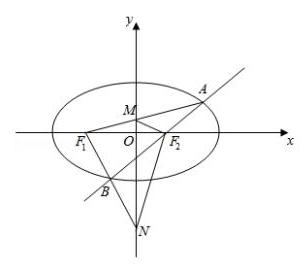
\includegraphics[max width=0.2\textwidth]{images/bo_d5jm9o77aajc7383vmi0_24_1156_1064_301_267_0.jpg}
\end{center}
\hspace*{3em} 

若 \({S}_{\bigtriangleup {F}_{1}{AB}} = {S}_{\bigtriangleup {F}_{1}{MN}}\) ,即 \(2\left| {{y}_{1} - {y}_{2}}\right|  = \left| {{y}_{3} - {y}_{4}}\right|\) ,

\(\left| {{y}_{3} - {y}_{4}}\right|  = \left| {\frac{2{y}_{1}}{{x}_{1} + 2} - \frac{2{y}_{2}}{{x}_{2} + 2}}\right|  = \left| {\frac{2{y}_{1}}{m{y}_{1} + 4} - \frac{2{y}_{2}}{m{y}_{2} + 4}}\right|\)

\(= \left| \frac{8\left( {{y}_{1} - {y}_{2}}\right) }{\left( {m{y}_{1} + 4}\right) \left( {m{y}_{2} + 4}\right) }\right|  = 2\left| {{y}_{1} - {y}_{2}}\right| ,\)

所以 \(\left| {\left( {m{y}_{1} + 4}\right) \left( {m{y}_{2} + 4}\right) }\right|  = 4,\left| {{m}^{2}{y}_{1}{y}_{2} + {4m}\left( {{y}_{1} + {y}_{2}}\right)  + {16}}\right|  = 4\) ,

代入根与系数的关系，得 \(\left| {\frac{-4{m}^{2}}{{m}^{2} + 2} + {4m} \cdot  \frac{-{4m}}{{m}^{2} + 2} + {16}}\right|  = 4\) ，解得 \(m = \; \pm  \sqrt{3}\) .

所以存在直线 \(x + \sqrt{3}y - 2 = 0\) 或 \(x - \sqrt{3}y - 2 = 0\) 满足题意. 2025 版上海高考真题及模拟训练合集(下册)

\section*{B、翻译简化运算大题}

【例题】1. (2023 上海春考) 椭圆 \(\Gamma  : \frac{{x}^{2}}{{m}^{2}} + \frac{{y}^{2}}{3} = 1\left( {m > 0,m \neq  \sqrt{3}}\right)\) .

(1)若 \(m = 2\) ，求椭圆 \(\Gamma\) 的离心率；

(2)设 \({A}_{1},{A}_{2}\) 为椭圆 \(\Gamma\) 的左右顶点，椭圆 \(\Gamma\) 上一点 \(E\) 的纵坐标为 1，且 \(\overrightarrow{E{A}_{1}} \cdot  \overrightarrow{E{A}_{2}} =  - 2\) ，求 \(m\) 的值;

(3) 过椭圆 \(\Gamma\) 上一点 \(P\) 作斜率为 \(\sqrt{3}\) 的直线，与双曲线 \(\frac{{y}^{2}}{5{m}^{2}} - \frac{{x}^{2}}{5} = 1\) 有一个公共点，求 \(m\) 的取值范围.

【解析】(1) 若 \(m = 2\) ,则 \(a = 2,{c}^{2} = 4 - 3 = 1\) ,所以 \(m = 2 \Rightarrow  a = 2,{c}^{2} = 4 - 3 = 1 \Rightarrow  c = 1 \Rightarrow\) ,离心率 \(\mathrm{e} \; = \frac{1}{2}\) ;

(2)法一:设 \(E\left( {{x}_{E},1}\right)\) ，代入椭圆 \(\Gamma  : \frac{{x}^{2}}{{m}^{2}} + \frac{{y}^{2}}{3} = 1\) 方程得 \({x}_{E} =  \pm  \frac{\sqrt{6}}{3}m\) .

由对称性,不妨设 \(M\left( {-\frac{\sqrt{6}}{3}m,1}\right) ,{A}_{1}\left( {-m,0}\right) ,{A}_{2}\left( {m,0}\right)\) ,

则 \(\overrightarrow{E{A}_{1}} \cdot  \overrightarrow{E{A}_{2}} = \left( {-m + \frac{\sqrt{6}}{3}m, - 1}\right)  \cdot  \left( {m + \frac{\sqrt{6}}{3}m, - 1}\right)  =  - 2\) ,

得 \(\left( {m + \frac{\sqrt{6}}{3}m, - 1}\right)  =  - 2 \Rightarrow  m = 3\) ;

法二: 设 \({A}_{1}\left( {-m,0}\right) ,{A}_{2}\left( {m,0}\right) ,E\left( {{x}_{0},1}\right)\) ,

则 \(\overrightarrow{E{A}_{1}} \cdot  \overrightarrow{E{A}_{2}} = \left( {\overrightarrow{EO} + \overrightarrow{O{A}_{1}}}\right)  \cdot  \left( {\overrightarrow{EO} + \overrightarrow{O{A}_{2}}}\right)  = {\overrightarrow{EO}}^{2} - \frac{1}{4}\overrightarrow{{A}_{1}{A}_{2}} =  - 2\) ,

得 \({x}_{0}^{2} + 1 - {m}^{2} =  - 2\) ,又点 \(E\) 在椭圆上,故 \(\frac{{x}_{0}^{2}}{{m}^{2}} + \frac{1}{3} = 1\) ,解得 \(m =  \pm  3\) ,

又 \(m > 0\) ,故 \(m = 3\) .

(3) 法一:设过点 \(P\) 的直线 \(l : y = \sqrt{3}x + t\) ，

由 \(\left\{  \begin{array}{l} y = \sqrt{3}x + t \\  \frac{{x}^{2}}{{m}^{2}} + \frac{{y}^{2}}{3} = 1 \end{array}\right.\) 得 \(\left( {3 + 3{m}^{2}}\right) {x}^{2} + 2\sqrt{3}t{m}^{2}x + \left( {{t}^{2} - 3}\right) {m}^{2} = 0\) ,

所以 \({\Delta }_{1} = {12}{t}^{2}{m}^{4} - 4\left( {3 + 3{m}^{2}}\right)  \cdot  \left( {{t}^{2} - 3}\right) {m}^{2} \geq  0 \Rightarrow  {t}^{2} \leq  3{m}^{2} + 3\)  \circled{1} ,

同理,由 \(\left\{  \begin{array}{l} y = \sqrt{3}x + t \\  \frac{{x}^{2}}{5{m}^{2}} - \frac{{y}^{2}}{5} = 1 \end{array}\right.\) 得 \(\left( {3 - {m}^{2}}\right) {x}^{2} + 2\sqrt{3}t{m}^{2}x + \left( {{t}^{2} - 5{m}^{2}}\right)  = 0\) ,

\({\Delta }_{2} = {12}{t}^{2} - 4\left( {3 - {m}^{2}}\right)  \cdot  \left( {{t}^{2} - 5{m}^{2}}\right)  = 0 \Rightarrow  {t}^{2} = 5{m}^{2} - {15}\)  \circled{2} ,

由 \circled{1}  \circled{2} 得 \(5{m}^{2} - {15} \leq  3{m}^{2} + 3 \Rightarrow  {m}^{2} \leq  9\) ，

又由 \circled{2} 得 \(\left\{  {\begin{array}{l} 5{m}^{2} - {15} \geq  0 \\  m \neq  \sqrt{3} \end{array} \Rightarrow  {m}^{2} > 3}\right.\) ，综上， \(m \in  (\sqrt{3},3\rbrack\) .

法二: 记过 \(P\) 所作的斜率为 \(\sqrt{3}\) 的直线为 \(l : y = \sqrt{3}x + t\) ,

对于双曲线 \(\frac{{y}^{2}}{5{m}^{2}} - \frac{{x}^{2}}{5} = 1\) ,其渐近线方程为 \(y =  \pm  {mx}\) ,又 \(m \neq  \sqrt{3}\) ,

故所作直线 \(l\) 不会与该渐近线平行或相交,

若 \(0 < m < \sqrt{3}\) 时,直线 \(l\) 与双曲线必有 2 个公共点;

若 \(m > \sqrt{3}\) 时,由 \(\left\{  \begin{array}{l} y = \sqrt{3}x + t \\  \frac{{y}^{2}}{5{m}^{2}} - \frac{{x}^{2}}{5} = 1 \end{array}\right.\) ,得 \(\left( {3 - {m}^{2}}\right) {x}^{2} + 2\sqrt{3}{tx} + {t}^{2} - 5{m}^{2} = 0\) ,

\({\Delta }_{1} = 0\) ,整理得 \({t}^{2} - 5{m}^{2} + {15} = 0\left( \mathrm{i}\right)\) ,

由 \(\left\{  \begin{array}{l} y = \sqrt{3}x + t \\  \frac{{x}^{2}}{{m}^{2}} + \frac{{y}^{2}}{3} = 1 \end{array}\right.\) ,得 \(\left( {3{m}^{2} + 3}\right) {x}^{2} + 2\sqrt{3}t{m}^{2}x + \left( {{t}^{2} - 3}\right) {m}^{2} = 0\) ,

\({\Delta }_{2} \geq  0\) ,整理得 \(3{m}^{2} - {t}^{2} + 3 \geq  0\left( {ii}\right)\) ,

由 (i) (ii) 得, \(m \leq  3\) ,故 \(\sqrt{3} < m \leq  3\) .

综上,实数 \(m\) 的取值范围是 \((\sqrt{3},3\rbrack\) .

【例题】2. (2022 上海秋考) 已知 \(\Gamma  : \frac{{x}^{2}}{{a}^{2}} + \frac{{y}^{2}}{{b}^{2}} = 1\left( {a > b > 0}\right)\) 的左、右焦点为 \({F}_{1}\left( {-\sqrt{2},0}\right) \text{ 、 }{F}_{2}\left( {\sqrt{2},0}\right)\) , \(A\) 为 \(\Gamma\) 的下顶点, \(M\) 为直线 \(l : x + y - 4\sqrt{2} = 0\) 上一点.

(1)若 \(a = 2,{AM}\) 的中点在 \(x\) 轴上，求点 \(M\) 的坐标；

(2)直线 \(l\) 交 \(y\) 轴于点 \(B\) ，直线 \({AM}\) 经过点 \({F}_{2}\) ，若 \(\bigtriangleup  {ABM}\) 有一个内角的余弦值为 \(\frac{3}{5}\) ，求 \(b\) ；

(3)若椭圆 \(\Gamma\) 上存在点 \(P\) 到直线 \(l\) 的距离为 \(d\) ，且满足 \(d + \left| {P{F}_{1}}\right|  + \left| {P{F}_{2}}\right|  = 6\) ，当 \(a\) 变化时，求 \(d\) 的最小值.

【解析】(1) 设 \(M\) 为 \(\left( {x,4\sqrt{2} - x}\right)\) ,线段 \({AM}\) 的中点坐标为 \(E\left( {\mathrm{e},0}\right)\) ,

由题意得 \(A\left( {0, - \sqrt{2}}\right)\) ,利用中点坐标公式得 \(x = 3\sqrt{2}\) ,所以有 \(M\left( {3\sqrt{2},\sqrt{2}}\right)\) ;

(2)情况一:当 \(\cos \angle {MAB} = \frac{3}{5}\) 时，有 \(\tan \angle {F}_{2}{AO} = \frac{O{F}_{2}}{OA} = \frac{4}{3} = \frac{\sqrt{2}}{b}\) ，

解得 \(b = \frac{3}{4}\sqrt{2}\) ，

情况二: 当 \(\cos \angle {AMB} = \frac{3}{5}\) 时，有 \(\cos \angle {MAB} = \cos \left( {\pi  - \angle {AMB} - \angle {ABM}}\right) \; \cos \angle {MAB} = \cos \left( {\pi  - \angle {AMB} - \angle {ABM}}\right)  =  - \cos \left( {\angle {AMB} + \angle {ABM}}\right)  =  - \left( {\frac{3}{5} \cdot  \frac{\sqrt{2}}{2} - \frac{4}{5} \cdot  \frac{\sqrt{2}}{2}}\right)  = \; \frac{\sqrt{2}}{10}\) ,

所以 \(\cos \angle {MAB} = \frac{\sqrt{2}}{10} = \frac{b}{\sqrt{2 + {b}^{2}}}\) ，解得 \(b = \frac{\sqrt{2}}{7}\) ，

综上所述， \(b = \frac{3}{4}\sqrt{2}\) 或 \(\frac{\sqrt{2}}{7}\) ；

(3)因为 \(d + \left| {P{F}_{1}}\right|  + \left| {P{F}_{2}}\right|  = 6\) ，所以 \(d + {2a} = 6\) ，即 \(d = 6 - {2a}\) ，

下面判断 \(a\) 的范围:

因为 \(d \geq  0\) ，所以 \(a \leq  3\) ，所以 \(\sqrt{2} < a \leq  3\) ，

设 \(P\left( {a\cos \alpha ,b\sin \alpha }\right)\) ,

得 \(d = \frac{\left| a\cos \alpha  + b\sin \alpha  - 4\sqrt{2}\right| }{\sqrt{2}} = \frac{\left| \sqrt{{a}^{2} + {b}^{2}}\sin \left( \alpha  + \varphi \right)  - 4\sqrt{2}\right| }{\sqrt{2}}\)

\(= \frac{\left| \sqrt{2{a}^{2} - 2}\sin \left( \alpha  + \varphi \right)  - 4\sqrt{2}\right| }{\sqrt{2}} = \left| {\sqrt{{a}^{2} - 1}\sin \left( {\alpha  + \varphi }\right)  - 4}\right| ,\)

因为 \(\sqrt{2} < a \leq  3\) ,所以 \(\sqrt{{a}^{2} - 1}\sin \left( {\alpha  + \varphi }\right)  < \sqrt{{a}^{2} - 1} \leq  2\sqrt{2} < 4\) ,

所以 \(d = 4 - \sqrt{{a}^{2} - 1}\sin \left( {\alpha  + \varphi }\right)  = 6 - {2a}\) ,

法一:若使得 \(d\) 最小，可令 \(\sin \left( {\alpha  + \varphi }\right)  = 1\) ，

此时 \({d}_{\min } = 4 - \sqrt{{a}^{2} - 1} = 6 - {2a}\) 是必要条件,解得 \(a = \frac{5}{3}\) ,

经检验 \(\frac{5}{3} \in  (\sqrt{2},3\rbrack\) ,所以 \({d}_{\min } = \frac{8}{3}\) .

法二: 因为 \(4 - \sqrt{{a}^{2} - 1} \leq  d = 6 - {2a} \leq  4 + \sqrt{{a}^{2} - 1}\) ,

所以 \({2a} - 2 \leq  \sqrt{{a}^{2} - 1}1 \leq  a \leq  \frac{5}{3}\) ，解得 \(\sqrt{2} < a \leq  \frac{5}{3}\) ，所以 \({d}_{\min } = \frac{8}{3}\) .

【例题】3. (2020 上海秋考)已知双曲线 \({\Gamma }_{1} : \frac{{x}^{2}}{4} - \frac{{y}^{2}}{{b}^{2}} = 1\) 与圆 \({\Gamma }_{2} : {x}^{2} + {y}^{2} = 4 + {b}^{2}\left( {b > 0}\right)\) 交于点 \(A\left( {x}_{A}\right.\) , \(\left. {y}_{A}\right)\) (第一象限),曲线 \(\Gamma\) 为 \({\Gamma }_{1}\text{ 、 }{\Gamma }_{2}\) 上取满足 \(x > \left| {x}_{A}\right|\) 的部分.

(1)若 \({x}_{A} = \sqrt{6}\) ，求 \(b\) 的值；

(2) 当 \(b = \sqrt{5},{\Gamma }_{2}\) 与 \(x\) 轴交点记作点 \({F}_{1}\text{ 、 }{F}_{2},P\) 是曲线 \(\Gamma\) 上一点,且在第一象限,且 \(\left| {P{F}_{1}}\right|  = 8\) ,求 \(\angle {F}_{1}P{F}_{2}\) ;

(3)过点 \(D\left( {0,\frac{{b}^{2}}{2} + 2}\right)\) 斜率为 \(- \frac{b}{2}\) 的直线 \(l\) 与曲线 \(\Gamma\) 只有两个交点,记为 \(M\text{ 、 }N\) ,用 \(b\) 表示 \(\overrightarrow{OM} \; \cdot  \overrightarrow{ON}\) ,并求 \(\overrightarrow{OM} \cdot  \overrightarrow{ON}\) 的取值范围.

【解析】(1) 由 \({x}_{A} = \sqrt{6}\) ,点 \(A\) 为曲线 \({\Gamma }_{1}\) 与曲线 \({\Gamma }_{2}\) 的交点,

联立 \(\left\{  \begin{array}{l} \frac{{x}_{A}^{2}}{4} - \frac{{y}_{A}^{2}}{{b}^{2}} = 1 \\  {x}_{A}^{2} + {y}_{A}^{2} = 4 + {b}^{2} \end{array}\right.\) ,解得 \({y}_{A} = \sqrt{2},b = 2\) ;

(2)由题意得 \({F}_{1}\text{ 、 }{F}_{2}\) 为曲线 \({\Gamma }_{1}\) 的两个焦点，

由双曲线的定义得 \(\left| {P{F}_{1}}\right|  - \left| {P{F}_{2}}\right|  = {2a}\) ,又 \(\left| {P{F}_{1}}\right|  = 8,{2a} = 4\) ,

所以 \(\left| {P{F}_{2}}\right|  = 8 - 4 = 4\) ,因为 \(b = \sqrt{5}\) ,则 \(c = \sqrt{4 + 5} = 3\) ,所以 \(\left| {{F}_{1}{F}_{2}}\right|  = 6\) ,

在 \(\bigtriangleup P{F}_{1}{F}_{2}\) 中,由余弦定理得 \(\cos \angle {F}_{1}P{F}_{2} = \frac{{\left| P{F}_{1}\right| }^{2} + {\left| P{F}_{2}\right| }^{2} - {\left| {F}_{1}{F}_{2}\right| }^{2}}{2\left| {P{F}_{1}}\right|  \cdot  \left| {P{F}_{2}}\right| }\)

\(= \frac{{64} + {16} - {36}}{2 \times  8 \times  4} = \frac{11}{16}\) ,由 \(0 < \angle {F}_{1}P{F}_{2} < \pi\) ,得 \(\angle {F}_{1}P{F}_{2} = \arccos \frac{11}{16}\) ;

(3) 设直线 \(l : y =  - \frac{b}{2}x + \frac{4 + {b}^{2}}{2}\) ，原点 \(O\) 到直线 \(l\) 的距离 \(d = \frac{\left| \frac{4 + {b}^{2}}{2}\right| }{\sqrt{1 + \frac{{b}^{2}}{4}}} = \sqrt{4 + {b}^{2}}\) ，

所以直线 \(l\) 是圆的切线,设切点为 \(M\) ,

所以 \({k}_{OM} = \frac{2}{b}\) ,并设 \({OM} : y = \frac{2}{b}x\) 与圆 \({x}^{2} + {y}^{2} = 4 + {b}^{2}\) 联立,

得 \({x}^{2} + \frac{4}{{b}^{2}}{x}^{2} = 4 + {b}^{2}\) ,得 \(x = b,y = 2\) ,即 \(M\left( {b,2}\right)\) ,

注意直线 \(l\) 与双曲线的斜率为负的渐近线平行,

所以只有当 \({y}_{A} > 2\) 时,直线 \(l\) 才能与曲线 \(\Gamma\) 有两个交点,

由 \(\left\{  \begin{array}{l} \frac{{x}_{A}^{2}}{4} - \frac{{y}_{A}^{2}}{{b}^{2}} = 1 \\  {x}_{A}^{2} + {y}_{A}^{2} = 4 + {b}^{2} \end{array}\right.\) ,得 \({y}_{A}^{2} = \frac{{b}^{4}}{a + {b}^{2}}\) ,

所以 \(4 < \frac{{b}^{4}}{4 + {b}^{2}}\) ,解得 \({b}^{2} > 2 + 2\sqrt{5}\) 或 \({b}^{2} < 2 - 2\sqrt{5}\) (舍去),

因为 \(\overrightarrow{OM}\) 为 \(\overrightarrow{ON}\) 在 \(\overrightarrow{OM}\) 上的投影，所以 \(\overrightarrow{OM} \cdot  \overrightarrow{ON} = 4 + {b}^{2}\) ，

所以 \(\overrightarrow{OM} \cdot  \overrightarrow{ON} = 4 + {b}^{2} > 6 + 2\sqrt{5}\) ,则 \(\overrightarrow{OM} \cdot  \overrightarrow{ON} \in  \left( {6 + 2\sqrt{5}, + \infty }\right)\) .

\begin{center}
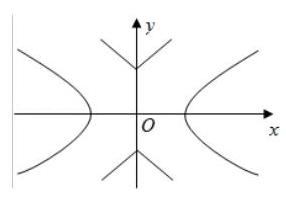
\includegraphics[max width=0.2\textwidth]{images/bo_d5jm9o77aajc7383vmi0_27_1175_1914_286_197_0.jpg}
\end{center}
\hspace*{3em} 

【例题】4. (2013 上海秋考) 如图,已知双曲线 \({C}_{1} : \frac{{x}^{2}}{2} - {y}^{2} = 1\) ,曲线 \({C}_{2} : \left| y\right|  = \; \left| x\right|  + 1,P\) 是平面内一点,若存在过点 \(P\) 的直线与 \({C}_{1},{C}_{2}\) 都有公共点,则称 \(P\) 为 “ \({C}_{1} - {C}_{2}\) 型点”

(1)在正确证明 \({C}_{1}\) 的左焦点是 “ \({C}_{1} - {C}_{2}\) 型点 “时，要使用一条过该焦点

的直线,试写出一条这样的直线的方程 (不要求验证);

(2) 设直线 \(y = {kx}\) 与 \({C}_{2}\) 有公共点,求证 \(\left| k\right|  > 1\) ，进而证明原点不是 “ \({C}_{1} - {C}_{2}\) 型点”；

(3) 求证: 圆 \({x}^{2} + {y}^{2} = \frac{1}{2}\) 内的点都不是 “ \({C}_{1} - {C}_{2}\) 型点”

【解析】 \(\left( 1\right) {C}_{1}\) 的左焦点为 \(\left( {-\sqrt{3},0}\right)\) ,写出的直线方程可以是以下形式:

\(x =  - \sqrt{3}\) 或 \(y = k\left( {x + \sqrt{3}}\right)\) ，其中 \(\left| k\right|  \geq  \frac{\sqrt{3}}{3}\) .

(2) 因为直线 \(y = {kx}\) 与 \({C}_{2}\) 有公共点，

所以方程组 \(\left\{  \begin{array}{l} y = {kx} \\  \left| y\right|  = \left| x\right|  + 1 \end{array}\right.\) 有实数解,因此 \(\left| {kx}\right|  = \left| x\right|  + 1\) ,得 \(\left| k\right|  = \frac{\left| x\right|  + 1}{\left| x\right| } > 1\) .

若原点是 “ \({C}_{1} - {C}_{2}\) 型点”,则存在过原点的直线与 \({C}_{1}\text{ 、 }{C}_{2}\) 都有公共点.

考虑过原点与 \({C}_{2}\) 有公共点的直线 \(x = 0\) 或 \(y = {kx}\left( {\left| k\right|  > 1}\right)\) .

显然直线 \(x = 0\) 与 \({C}_{1}\) 无公共点.

如果直线为 \(y = {kx}\left( {\left| k\right|  > 1}\right)\) ,由 \(\left\{  \begin{array}{l} y = {kx} \\  \frac{{x}^{2}}{2} - {y}^{2} = 1 \end{array}\right.\) ,得 \({x}^{2} = \frac{2}{1 - 2{k}^{2}} < 0\) ,矛盾.

所以直线 \(y = {kx}\left( {\left| k\right|  > 1}\right)\) 与 \({C}_{1}\) 也无公共点,因此原点不是 “ \({C}_{1} - {C}_{2}\) 型点”.

(3) 记圆 \(O : {x}^{2} + {y}^{2} = \frac{1}{2}\) ,取圆 \(O\) 内的一点 \(Q\) ,

设有经过 \(Q\) 的直线 \(l\) 与 \({C}_{1}\text{ 、 }{C}_{2}\) 都有公共点,显然 \(l\) 不与 \(x\) 轴垂直,

故可设 \(l : y = {kx} + b\) .

若 \(\left| k\right|  \leq  1\) ,由于圆 \(O\) 夹在两组平行线 \(y = x \pm  1\) 与 \(y =  - x \pm  1\) 之间,

因此圆 \(O\) 也夹在直线 \(y = {kx} \pm  1\) 与 \(y =  - {kx} \pm  1\) 之间，

从而过 \(Q\) 且以 \(k\) 为斜率的直线 \(l\) 与 \({C}_{2}\) 无公共点,矛盾,所以 \(\left| k\right|  > 1\) .

因为 \(l\) 与 \({C}_{1}\) 由公共点,所以方程组 \(\left\{  \begin{array}{l} y = {kx} + b \\  \frac{{x}^{2}}{2} - {y}^{2} = 1 \end{array}\right.\) 有实数解,

得 \(\left( {1 - 2{k}^{2}}\right) {x}^{2} - {4kbx} - 2{b}^{2} - 2 = 0\) .

因为 \(\left| k\right|  > 1\) ,所以 \(1 - 2{k}^{2} \neq  0\) ,

因此 \(\Delta  = {\left( 4kb\right) }^{2} - 4\left( {1 - 2{k}^{2}}\right) \left( {-2{b}^{2} - 2}\right)  = 8\left( {{b}^{2} + 1 - 2{k}^{2}}\right)  \geq  0\) ,即 \({b}^{2} \geq  2{k}^{2} - 1\) .

因为圆 \(O\) 的圆心 \(\left( {0,0}\right)\) 到直线 \(l\) 的距离 \(d = \frac{\left| b\right| }{\sqrt{1 + {k}^{2}}}\) ,

所以 \(\frac{{b}^{2}}{1 + {k}^{2}} = {d}^{2} < \frac{1}{2}\) ,从而 \(\frac{1 + {k}^{2}}{2} > {b}^{2} \geq  2{k}^{2} - 1\) ,得 \({k}^{2} < 1\) ,与 \(\left| k\right|  > 1\) 矛盾.

因此圆 \({x}^{2} + {y}^{2} = \frac{1}{2}\) 内的点不是 “ \({C}_{1} - {C}_{2}\) 型点”.

【例题】5. (2010 上海春考) 在平面上,给定非零向量 \(\overrightarrow{b}\) ,对任意向量 \(\overrightarrow{a}\) ,定义 \(\overrightarrow{{a}^{\prime }} = \overrightarrow{a} - \frac{2\left( {\overrightarrow{a} \cdot  \overrightarrow{b}}\right) }{{\left| \overrightarrow{b}\right| }^{2}}\overrightarrow{b}\) .

(1) 若 \(\overrightarrow{a} = \left( {2,3}\right) ,\overrightarrow{b} = \left( {-1,3}\right)\) ,求 \(\overrightarrow{{a}^{\prime }}\) ;

( 2 )若 \(\overrightarrow{b} = \left( {2,1}\right)\) ，证明:若位置向量 \(\overrightarrow{a}\) 的终点在直线 \({Ax} + {By} + C = 0\) 上，则位置向量 \(\overrightarrow{{a}^{\prime }}\) 的终点也在一条直线上;

(3)已知存在单位向量 \(\overrightarrow{b}\) ，当位置向量 \(\overrightarrow{a}\) 的终点在抛物线 \(C : {x}^{2} = y\) 上时，位置向量 \(\overrightarrow{{a}^{\prime }}\) 终点总在抛物线 \({C}^{\prime } : {y}^{2} = x\) 上,曲线 \(C\) 和 \({C}^{\prime }\) 关于直线 \(l\) 对称,问直线 \(l\) 与向量 \(\overrightarrow{b}\) 满足什么关系?

【解析】(1) 因为 \(\overrightarrow{a} = \left( {2,3}\right) ,\overrightarrow{b} = \left( {-1,3}\right)\) ,

所以 \(\overrightarrow{a} \cdot  \overrightarrow{b} = 7,{\left| \overrightarrow{b}\right| }^{2} = {10}\) ,得 \(\frac{2\left( {\overrightarrow{a} \cdot  \overrightarrow{b}}\right) }{{\left| \overrightarrow{b}\right| }^{2}}\overrightarrow{b} = \frac{2 \times  7}{10}\left( {-1,3}\right)  = \left( {-\frac{7}{5},\frac{21}{5}}\right)\) ,

因此 \(\overrightarrow{{a}^{\prime }} = \overrightarrow{a} - \frac{2\left( {\overrightarrow{a} \cdot  \overrightarrow{b}}\right) }{{\left| \overrightarrow{b}\right| }^{2}}\overrightarrow{b} = \left( {2,3}\right)  - \left( {-\frac{7}{5},\frac{21}{5}}\right)  = \left( {\frac{17}{5}, - \frac{6}{5}}\right)\) ;

(2)设 \(\overrightarrow{a} = \left( {{x}^{\prime },{y}^{\prime }}\right)\) ，终点在直线 \({Ax} + {By} + C = 0\) 上，

则 \(\overrightarrow{a} \cdot  \overrightarrow{b} = 2{x}^{\prime } + {y}^{\prime },{\left| \overrightarrow{b}\right| }^{2} = 5\) ，

\(\frac{2\left( {\overrightarrow{a} \cdot  \overrightarrow{b}}\right) }{{\left| \overrightarrow{b}\right| }^{2}}\overrightarrow{b} = \frac{2\left( {2{x}^{\prime } + {y}^{\prime }}\right) }{5}\left( {2,1}\right)  = \left( {\frac{8{x}^{\prime } + 4{y}^{\prime }}{5},\frac{4{x}^{\prime } + 2{y}^{\prime }}{5}}\right) ,\)

所以 \(\overrightarrow{{a}^{\prime }} = \overrightarrow{a} - \frac{2\left( {\overrightarrow{a} \cdot  \overrightarrow{b}}\right) }{{\left| \overrightarrow{b}\right| }^{2}}\overrightarrow{b} = \left( {{x}^{\prime },{y}^{\prime }}\right)  - \left( {\frac{8{x}^{\prime } + 4{y}^{\prime }}{5},{y}^{\prime }}\right)  - \left( {\frac{8{x}^{\prime } + 4{y}^{\prime }}{5},\frac{4{x}^{\prime } + 2{y}^{\prime }}{5}}\right)  = \; \left( {\frac{-3{x}^{\prime } - 4{y}^{\prime }}{5},\frac{-4{x}^{\prime } + 3{y}^{\prime }}{5}}\right) ,\)

因此,若 \(\overrightarrow{{a}^{\prime }} = \left( {x,y}\right)\) ,满足 \(\left\{  \begin{array}{l} x = \frac{-3{x}^{\prime } - 4{y}^{\prime }}{5} \\  y = \frac{-4{x}^{\prime } + 3{y}^{\prime }}{5} \end{array}\right.\) ,得 \(\left\{  \begin{array}{l} {x}^{\prime } = \frac{-{3x} - {4y}}{5} \\  {y}^{\prime } = \frac{-{4x} + {3y}}{5} \end{array}\right.\) ,

因为点 \(\left( {\frac{-{3x} - {4y}}{5},\frac{-{4x} + {3y}}{5}}\right)\) 在直线 \({Ax} + {By} + C = 0\) 上,

所以 \(A \times  \frac{-{3x} - {4y}}{5} + B \times  \frac{-{4x} + {3y}}{5} + C = 0\) ,

化简得 \(\left( {{3A} + {4B}}\right) x + \left( {{4A} - {3B}}\right) y - {5C} = 0\) ,

由 \(A\text{ 、 }B\) 不全为零,得以上方程是一条直线的方程

即向量 \(\overrightarrow{{a}^{\prime }}\) 的终点也在一条直线上;

(3)因为 \(\overrightarrow{b}\) 是单位向量，

所以设 \(\overrightarrow{a} = \left( {x,y}\right) ,\overrightarrow{b} = \left( {\cos \theta ,\sin \theta }\right)\) ,得 \(\overrightarrow{a} \cdot  \overrightarrow{b} = x\cos \theta  + y\sin \theta\) ,

所以 \(\overrightarrow{{a}^{\prime }} = \overrightarrow{a} - \frac{2\left( {\overrightarrow{a} \cdot  \overrightarrow{b}}\right) }{{\left| \overrightarrow{b}\right| }^{2}}\overrightarrow{b} = \overrightarrow{a} - 2\left( {x\cos \theta  + y\sin \theta }\right) \overrightarrow{b}\)

\(= \left( {-x\cos {2\theta } - y\sin {2\theta }, - x\sin {2\theta } + y\cos {2\theta }}\right)\) ,

因为 \(\overrightarrow{a}\) 的终点在抛物线 \({x}^{2} = y\) 上,且 \(\overrightarrow{{a}^{\prime }}\) 终点在抛物线 \({y}^{2} = x\) 上,

所以 \(- x\cos {2\theta } - y\sin {2\theta } = {\left( -x\sin 2\theta  + y\cos 2\theta \right) }^{2}\) ,

化简整理,通过比较系数得 \(\cos \theta  = \frac{\sqrt{2}}{2},\sin \theta  =  - \frac{\sqrt{2}}{2}\)

或 \(\cos \theta  =  - \frac{\sqrt{2}}{2},\sin \theta  = \frac{\sqrt{2}}{2}\) ,所以 \(\overrightarrow{b} =  \pm  \left( {-\frac{\sqrt{2}}{2},\frac{\sqrt{2}}{2}}\right)\) ,

因为曲线 \(C\) 和 \({C}^{\prime }\) 关于直线 \(l : y = x\) 对称,所以 \(l\) 的方向向量 \(\overrightarrow{d} = \left( {1,1}\right)\) .

得 \(\overrightarrow{d} \cdot  \overrightarrow{b} = 0\) ,即 \(\overrightarrow{d} \bot  \overrightarrow{b}\) ,因此直线 \(l\) 与向量 \(\overrightarrow{b}\) 垂直. 2025 版上海高考真题及模拟训练合集(下册)

\section*{C、参数方程计算大题}

【例题】1. (2025 上海春考) 在平面直角坐标系中,已知曲线 \(\Gamma  : \frac{{x}^{2}}{4} + {y}^{2} = 1\left( {y \geq  0}\right)\) ,点 \(P,Q\) 分别为 \(\Gamma\) 上不同的两点, \(T\left( {t,0}\right)\) .

(1)求 \(\Gamma\) 所在椭圆的离心率；

(2)若 \(T\left( {1,0}\right)\) ， \(Q\) 在 \(y\) 轴上，若 \(T\) 到直线 \({PQ}\) 的距离为 \(\frac{\sqrt{5}}{5}\) ，求 \(P\) 的坐标；

(3) 是否存在 \(t\) ，使得 \(\bigtriangleup  {TPQ}\) 是以 \(T\) 为直角顶点的等腰直角三角形？若存在，求 \(t\) 的取值范围； 若不存在，请说明理由.

\begin{center}
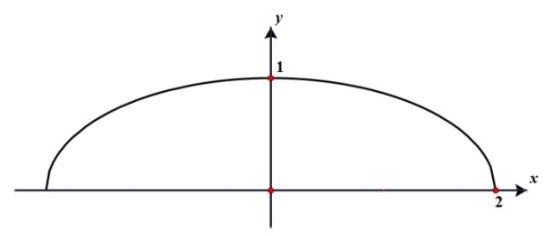
\includegraphics[max width=0.4\textwidth]{images/bo_d5jm9o77aajc7383vmi0_30_328_601_547_236_0.jpg}
\end{center}
\hspace*{3em} 

【解析】(1) 由题意得, \(a = 2,c = \sqrt{3}\) ,所以椭圆的离心率 \(\mathrm{e} = \frac{\sqrt{3}}{2}\) ;

(2) 由题意得,点 \(Q\) 的坐标为 \(\left( {0,1}\right)\) ,设点 \(T\) 到直线 \({PQ}\) 的距离为 \(d\) .

当直线 \({PQ}\) 的斜率不存在时, \(d = 1\) ,不合题意;

当直线 \({PQ}\) 的斜率存在时,设 \({PQ}\) 的方程为 \(y = {kx} + 1\) ,则 \(d = \frac{\left| k + 1\right| }{\sqrt{{k}^{2} + 1}} = \frac{\sqrt{5}}{5}\) ,解得 \(k =  - 2\) 或 \(k \; =  - \frac{1}{2}\) .

当 \(k =  - 2\) 时,联立 \(\left\{  \begin{array}{l} y =  - {2x} + 1 \\  {x}^{2} + 4{y}^{2} = 4 \end{array}\right.\) ,解得 \(\left\{  \begin{array}{l} x = 0 \\  y = 1 \end{array}\right.\) 或 \(\left\{  \begin{array}{l} x = \frac{16}{17} \\  y =  - \frac{15}{17} \end{array}\right.\) ,不符合题意,舍去;

当 \(k =  - \frac{1}{2}\) 时,联立 \(\left\{  \begin{array}{l} y =  - \frac{1}{2}x + 1 \\  {x}^{2} + 4{y}^{2} = 4 \end{array}\right.\) ,解得 \(\left\{  \begin{array}{l} x = 0 \\  y = 1 \end{array}\right.\) 或 \(\left\{  \begin{array}{l} x = 2 \\  y = 0 \end{array}\right.\) ,符合题意;

综上所述: 点 \(P\) 的坐标为 \(\left( {2,0}\right)\) .

(3) 存在.

法一:不妨设点 \(P\) 在点 \(Q\) 的右侧，设 \(\left| {PT}\right|  = \left| {QT}\right|  = r\) ，直线 \({PT}\) 的倾斜角为 \(\alpha  \in  \left\lbrack  {0,\frac{\pi }{2}}\right\rbrack\) ，则点 \(P\) 的坐标为 \(\left( {t + r\cos \alpha ,r\sin \alpha }\right)\) ,点 \(Q\) 的坐标为 \(\left( {t - r\sin \alpha ,r\cos \alpha }\right)\) .

将点 \(P,Q\) 的坐标代入椭圆方程,得 \(\left\{  \begin{array}{l} {\left( t + r\cos \alpha \right) }^{2} + 4{r}^{2}{\sin }^{2}\alpha  = 4\cdots \\  {\left( t - r\sin \alpha \right) }^{2} + 4{r}^{2}{\cos }^{2}\alpha  = 4\cdots  \end{array}\right.\) \circled{1}   \circled{2} 

 \circled{1} - \circled{2} ，得 \(3\left( {\cos \alpha  - \sin \alpha }\right) r = {2t}\) .

当 \(\alpha  = \frac{\pi }{4}\) 时， \(t = 0\) ；当 \(\alpha  \neq  \frac{\pi }{4}\) 时， \(r = \frac{2t}{3\left( {\cos \alpha  - \sin \alpha }\right) }\)

 \circled{1}  +  \circled{2} ,得 \(2{t}^{2} + {2tr}\left( {\cos \alpha  - \sin \alpha }\right)  + 5{r}^{2} = 8\cdots \cdots\)  \circled{4} 

将 \circled{3} 代入 \circled{4} ，化简得 \({t}^{2} = \frac{36}{{15} + \frac{10}{{\left( \cos \alpha  - \sin \alpha \right) }^{2}}}\) .

又 \(\alpha  \in  \left\lbrack  {0,\frac{\pi }{2}}\right\rbrack\) ,所以 \({\left( \cos \alpha  - \sin \alpha \right) }^{2} \in  (0,1\rbrack\) ,所以 \({t}^{2} \leq  \frac{36}{{15} + {10}} = \frac{36}{25}\) ,解得 \(t \in  \left\lbrack  {-\frac{6}{5},\frac{6}{5}}\right\rbrack\) .

法二:不妨设点 \(P\) 在点 \(Q\) 的右侧，设 \(\overrightarrow{TP} = \left( {m,n}\right)\) ， \(\overrightarrow{TQ} = \left( {-n,m}\right)\) ，其中 \(m \geq  0\) ， \(n \geq  0\) ， 则点 \(P\) 的坐标为 \(\left( {t + m,n}\right)\) ，点 \(Q\) 的坐标为 \(\left( {t - n,m}\right)\) .

将点 \(P,Q\) 代入椭圆方程,得 \(\left\{  \begin{array}{l} {\left( t + m\right) }^{2} + 4{n}^{2} = 4\cdots \cdots \left( 1\right) \\  {\left( t - n\right) }^{2} + 4{m}^{2} = 4\cdots \cdots \left( 2\right)  \end{array}\right.\)

 \circled{1} - \circled{2} ，得 \(m - n = \frac{2}{3}t\) ，将 \(m = \frac{2}{3}t + n\) 代入  \circled{1} ，化简得 \({n}^{2} + \frac{2}{3}{tn} + \frac{5}{9}{t}^{2} - \frac{4}{5} = 0\) .

设该方程的两根 \({n}_{1},{n}_{2}\) ,则 \({n}_{1} + {n}_{2} =  - \frac{2}{3}t = n - m\) ,因此该方程的两根为 \(n, - m\) ,所以两根之积 \(- {nm} = {n}_{1} \cdot  {n}_{2} = \frac{5}{9}{t}^{2} - \frac{4}{5} \leq  0\) ,解得 \(t \in  \left\lbrack  {-\frac{6}{5},\frac{6}{5}}\right\rbrack\) . 经检验，此时判别式大于零.

综上所述: \(t \in  \left\lbrack  {-\frac{6}{5},\frac{6}{5}}\right\rbrack\) .

法三: (填选题可用,极限思想) 不妨设点 \(P\) 在点 \(Q\) 的右侧,当点 \(T\) 从左侧非常靠近长轴右端点时,显然图中 \(\left| {PT}\right|  < \left| {QT}\right|\) ,因此我们只要计算当点 \(P\) 刚好在长轴右端点时,点 \(T\) 位于何处,能刚好形成等腰直角三角形 (临界状态).

此时则点 \(T\) 的坐标为 \(\left( {t,0}\right)\) ,点的 \(P\) 坐标为 \(\left( {2,0}\right)\) ,点 \(Q\) 的坐标为 \(\left( {t,\sqrt{1 - \frac{{t}^{2}}{4}}}\right)\) ,所以 \(2 - t = \; \sqrt{1 - \frac{{t}^{2}}{4}}\) ,解得 \(t = \frac{6}{5}\) ,所以答案为 \(t \in  \left\lbrack  {-\frac{6}{5},\frac{6}{5}}\right\rbrack\) .

法四: 设直线 \({l}_{PQ} : x = {my} + n\) ,(反设是因为 \({y}_{1},{y}_{2} \geq  0\) ,需要得到关于 \(y\) 的方程)

与曲线 \(\Gamma\) 联立,有 \(\left\{  {\begin{array}{l} x = {my} + n \\  \frac{{x}^{2}}{4} + {y}^{2} = 1 \end{array} \Rightarrow  \left( {{m}^{2} + 4}\right) {y}^{2} + {2mny} + {n}^{2} - 4 = 0}\right.\)

\(\Delta  = {16}\left( {{m}^{2} - {n}^{2} + 4}\right) ,{y}_{1} + {y}_{2} = \frac{-{2mn}}{{m}^{2} + 4} > 0,{y}_{1}{y}_{2} = \frac{{n}^{2} - 4}{{m}^{2} + 4} \geq  0 \Rightarrow  {n}^{2} \geq  4\)

且中点 \(M\left( {\frac{4n}{{m}^{2} + 4},\frac{-{mn}}{{m}^{2} + 4}}\right)\) ,则 \({k}_{TM} = \frac{\frac{-{mn}}{{m}^{2} + 4}}{\frac{4n}{{m}^{2} + 4} - t} =  - m\) ,

化简后得: \(\left( {{m}^{2} + 4}\right) t = {3n}\) ,即 \({m}^{2} + 4 = \frac{3n}{t}\)

同时, \({PQ} = {2MT} = {2d}\)

而 \({PQ} = \sqrt{1 + {m}^{2}} \cdot  \frac{4 \cdot  \sqrt{{m}^{2} - {n}^{2} + 4}}{{m}^{2} + 4},{MT} = {2d} = 2\frac{\left| t - n\right| }{\sqrt{1 + {m}^{2}}}\)

所以 \(\sqrt{1 + {m}^{2}} \cdot  \frac{4 \cdot  \sqrt{{m}^{2} - {n}^{2} + 4}}{{m}^{2} + 4} = 2\frac{\left| t - n\right| }{\sqrt{1 + {m}^{2}}}\)

即 \(2\left( {1 + {m}^{2}}\right) \frac{\sqrt{{m}^{2} - {n}^{2} + 4}}{{m}^{2} + 4} = \left| {t - n}\right|\) ,

因为 \(n\) 有范围,所以下面需消去 \(m\) ,建立 \(n,t\) 的直接关系式

则 \(2\left( {\frac{3n}{t} - 3}\right) \frac{\sqrt{\frac{3n}{t} - {n}^{2}}}{\frac{3n}{t}} = \left| {t - n}\right|\)

即 \(2\left( {n - t}\right) \sqrt{\frac{{3n} - t{n}^{2}}{t}} = \left| {t - n}\right|  \cdot  n\) ,

平方后得, \(t = \frac{12}{5n}\) ,因为 \(\left| n\right|  \geq  2\) ,所以 \(t \in  \left\lbrack  {-\frac{5}{6},0}\right)  \cup  \left( {0,\frac{5}{6}}\right\rbrack\)

又因为 \(t = 0\) 显然成立,所以 \(t \in  \left\lbrack  {-\frac{5}{6},\frac{5}{6}}\right\rbrack\)

如图，不妨设点 \(P\left( {2\cos \alpha ,\sin \alpha }\right)\) ， \(Q\left( {2\cos \beta ,\sin \beta }\right)\) ， \(\left( {0 \leq  \alpha  < \beta  \leq  \pi }\right)\) ，

点 \(A\) 、 \(B\) 是点 \(P\) 、 \(Q\) 在 \(x\) 轴上的投影，

\begin{center}
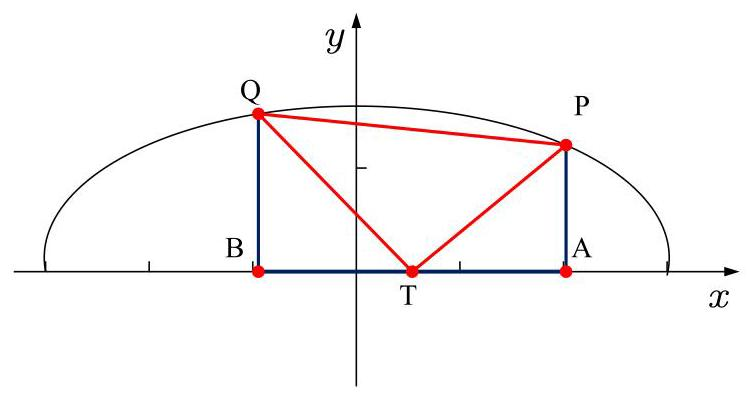
\includegraphics[max width=0.6\textwidth]{images/bo_d5jm9o77aajc7383vmi0_32_294_260_747_394_0.jpg}
\end{center}
\hspace*{3em} 

因为 \(\bigtriangleup {PTQ}\) 是等腰直角三角形,所以可得 \(\bigtriangleup {PAT} \cong  \bigtriangleup {TBQ}\) ,

因此 \(\left| {AT}\right|  = \left| {BQ}\right| ,\left| {AP}\right|  = \left| {BT}\right|\) ,于是 \(\left\{  \begin{array}{l} 2\cos \alpha  - t = \sin \beta ,\left( 1\right) \\  t - 2\cos \beta  = \sin \alpha ,\left( 2\right)  \end{array}\right.\) ,

两式相加可得: \(2\cos \alpha  - 2\cos \beta  = \sin \alpha  + \sin \beta\) ,

由和差化积公式可得: \(- 4\sin \frac{\alpha  + \beta }{2}\sin \frac{\alpha  - \beta }{2} = \sin \frac{\alpha  + \beta }{2}\cos \frac{\alpha  - \beta }{2}\) ,

由 \(0 < \frac{\beta  + \alpha }{2} < \pi ,0 < \beta  - \alpha  < \pi\) ,可知

\(\tan \frac{\beta  - \alpha }{2} = \frac{1}{2} \Rightarrow  \sin \left( {\beta  - \alpha }\right)  = \frac{4}{5},\cos \left( {\beta  - \alpha }\right)  = \frac{3}{5}\) ,且 \(\beta  - \alpha  = \arccos \frac{3}{5}\) ,

由 (1) 式可得: \(t = 2\cos \alpha  - \sin \beta  = 2\cos \left( {\alpha  - \beta }\right)  + \beta  - \sin \beta\)

\(= 2\cos \left( {\alpha  - \beta }\right) \cos \beta  - 2\sin \left( {\alpha  - \beta }\right) \sin \beta  - \sin \beta\)

\(= \frac{3}{5}\sin \beta  + \frac{6}{5}\cos \beta\)

由辅助角公式可知: \(t = \frac{3\sqrt{5}}{5}\sin \left( {\beta  + \arctan 2}\right)\) ;

因为 \(\beta  - \alpha  = \arccos \frac{3}{5}\) ,所以 \(\arccos \frac{3}{5} \leq  \beta  \leq  \pi\) ,且 \(\frac{\pi }{2} < \beta  + \arctan 2 < \frac{3\pi }{2}\) ,

于是 \(t = \frac{3\sqrt{5}}{5}\sin \left( {\beta  + \arctan 2}\right)\) 是 \(\beta\) 的严格减函数,

当 \(\cos \beta  = \frac{3}{5},\sin \beta  = \frac{4}{5}\) 时, \({t}_{\max } = \frac{3}{5}\sin \beta  + \frac{6}{5}\cos \beta  = \frac{3}{5} \times  \frac{4}{4} + \frac{6}{5} \times  \frac{3}{5} = \frac{6}{5}\) ;

当 \(\cos \beta  =  - 1,\sin \beta  = 0\) 时, \({t}_{\min } = \frac{3}{5}\sin \beta  + \frac{6}{5}\cos \beta  = \frac{3}{5} \times  0 + \frac{6}{5} \times  \left( {-1}\right)  =  - \frac{6}{5}\) ;

因此 \(t \in  \left\lbrack  {-\frac{6}{5},\frac{6}{5}}\right\rbrack\) .

【例题】2. (2022 上海春考) 椭圆 \(\Gamma  : \frac{{x}^{2}}{{a}^{2}} + {y}^{2} = 1\left( {a > 1}\right) ,A,B\) 分别为椭圆的左顶点和下顶点,且直线 \(x \; = a\) 上有两个不相同的点 \(C,D(C\) 是第一象限的点).

(1)设 \(F\) 是椭圆 \(\Gamma\) 的右焦点,且 \(\angle {AFB} = \frac{\pi }{6}\) ，求椭圆 \(\Gamma\) 的标准方程；

(2)若 \(C\) ， \(D\) 两点的纵坐标分别为2和1，判断:直线 \({BC}\) 与 \({AD}\) 的交点是否在椭圆 \(\Gamma\) 上，并说明理由;

(3) 设直线 \({AD}\) 与直线 \({BC}\) 交椭圆 \(\Gamma\) 于 \(P,Q\) 两点，且 \(P,Q\) 关于原点对称，求 \(\left| {CD}\right|\) 的最小值.

【解析】(1) 因为 \(\angle {AFB} = \frac{\pi }{6},{OB} = 1\) ，所以 \({OF} = \sqrt{3}\) ，所以 \(a = \sqrt{{\left( \sqrt{3}\right) }^{2} + 1} = 2\) ，

所以椭圆 \(\Gamma\) 的标准方程为 \(\frac{{x}^{2}}{4} + {y}^{2} = 1\) ;

(2) 由题意得 \(A\left( {-a,0}\right) ,B\left( {0, - 1}\right) ,C\left( {a,2}\right) ,D\left( {a,1}\right)\) ,

直线 \({AD}\) 的方程为 \(y - 0 = \frac{1}{2a}\left( {x + a}\right)\) ,即 \(y = \frac{1}{2a}x + \frac{1}{2}\) ,

直线 \({BC}\) 的方程为 \(y + 1 = \frac{3}{a}\left( {x - 0}\right)\) ,即 \(y = \frac{3}{a}x - 1\) ,

由 \(\left\{  \begin{array}{l} y = \frac{1}{2a}x + \frac{1}{2} \\  y = \frac{3}{a}x - 1 \end{array}\right.\) 得 \(\left\{  \begin{array}{l} x = \frac{3}{5}a \\  y = \frac{4}{5} \end{array}\right.\) ,因为 \(\frac{{\left( \frac{3}{5}a\right) }^{2}}{{a}^{2}} + {\left( \frac{4}{5}\right) }^{2} = 1\) ,

所以直线 \({BC}\) 与 \({AD}\) 的交点在椭圆 \(\Gamma\) 上;

(3) 法一:设 \(C\left( {a,m}\right)\) ， \(D\left( {a,n}\right)\) ，其中 \(m > 0\) ，即求 \(\left| {m - n}\right|\) 的最小值.

直线 \({AD}\) 方程为 \(y = \frac{n}{2a}\left( {x + a}\right)\) ，直线 \({BC}\) 方程为 \(y = \frac{m + 1}{a}x - 1\) ，

设 \({AD}\) 与 \(\Gamma\) 交点为 \(P\) ,由 \(\left\{  \begin{array}{l} \frac{{x}^{2}}{{a}^{2}} + {y}^{2} = 1 \\  y = \frac{n}{2a}\left( {x + a}\right)  \end{array}\right.\) 得 \(\frac{{x}^{2}}{{a}^{2}} + \frac{{n}^{2}}{4{a}^{2}}{\left( x + a\right) }^{2} = 1\) ,

整理得 \(\left( {\frac{1}{{a}^{2}} + \frac{{n}^{2}}{4{a}^{2}}}\right) {x}^{2} + \frac{{n}^{2}}{2a}x + \frac{{n}^{2}}{4} - 1 = 0\) ,

由韦达定理得 \(- a \cdot  {x}_{P} = \frac{\frac{{n}^{2}}{4} - 1}{\frac{1}{{a}^{2}} + \frac{{n}^{2}}{4{a}^{2}}} = \frac{{a}^{2}{n}^{2} - 4{a}^{2}}{4 + {n}^{2}}\) ,则 \({x}_{P} = \frac{{4a} - a{n}^{2}}{4 + {n}^{2}}\) ,

设 \({BC}\) 与 \(\Gamma\) 交点为 \(Q\) ,由 \(\left\{  \begin{array}{l} \frac{{x}^{2}}{{a}^{2}} + {y}^{2} = 1 \\  y = \frac{m + 1}{a}x - 1 \end{array}\right.\) 得 \(\left\lbrack  {\frac{1}{{a}^{2}} + \frac{{\left( m + 1\right) }^{2}}{{a}^{2}}}\right\rbrack  {x}^{2} - \frac{{2m} + 2}{a}x = 0\) ,得 \({x}_{Q} = \; \frac{\frac{{2m} + 2}{a}}{\frac{1}{{a}^{2}} + \frac{{\left( m + 1\right) }^{2}}{{a}^{2}}}\) ,即 \({x}_{Q} = \frac{{2a}\left( {m + 1}\right) }{{m}^{2} + {2m} + 2}\) ,

又 \(P,Q\) 关于原点对称,所以 \(\frac{{4a} - a{n}^{2}}{4 + {n}^{2}} + \frac{{2a}\left( {m + 1}\right) }{{m}^{2} + {2m} + 2} = 0\) ,

即 \(\frac{4 - {n}^{2}}{4 + {n}^{2}} = \frac{-2\left( {m + 1}\right) }{{\left( m + 1\right) }^{2} + 1}\) ,得 \(\left\{  \begin{array}{l} \frac{8}{4 + {n}^{2}} = \frac{{\left( m + 1 - 1\right) }^{2}}{{\left( m + 1\right) }^{2} + 1} \\  \frac{2{n}^{2}}{4 + {n}^{2}} = \frac{{\left( m + 1 + 1\right) }^{2}}{{\left( m + 1\right) }^{2} + 1} \end{array}\right.\) ,即 \(\frac{8}{2{n}^{2}} = \frac{{m}^{2}}{{\left( m + 2\right) }^{2}}\) ,

所以 \(\pm  \frac{2}{n} = \frac{m}{m + 2}\) .

考虑到 \(Q\) 在第一象限,则有 \(P\) 在第三象限,那么必有 \(n < 0\) ,

所以 \(- \frac{2}{n} = \frac{m + 2}{m}\) ,那么 \(n =  - \frac{{2m} + 4}{m}\) ,

所以 \(m - n = m + \frac{{2m} + 4}{m} = m + \frac{4}{m} + 2 \geq  6\) ,当且仅当 \(m = 2\) 时取等号,

此时 \(n =  - 4\) ,故 \(\left| {CD}\right|\) 的最小值为 6 ;

法二: 设直线 \({AD}\) 为 \(x + {my} + a = 0\) ,与椭圆交于点 \(P\) ,

由 \(\left\{  \begin{array}{l} \frac{{x}^{2}}{{a}^{2}} + {y}^{2} = 1 \\  x + {my} + a = 0 \end{array}\right.\) 得 \(\left( {\frac{{m}^{2}}{{a}^{2}} + 1}\right) {y}^{2} + \frac{2m}{a}y = 0\) ,那么 \({y}_{P} = \frac{-{2ma}}{{m}^{2} + {a}^{2}}\) ,

得 \({x}_{P} = \frac{a\left( {{m}^{2} - {a}^{2}}\right) }{{a}^{2} + {m}^{2}}\) ,在 \(x + {my} + a = 0\) 中,令 \(x = a\) 得 \(D\left( {a, - \frac{2a}{m}}\right)\) ,

考虑到 \(P\) 在第三象限,则 \(a > m > 0\) ,

设直线 \({BC}\) 为 \(y = {kx} - 1\) ，与椭圆交于点 \(Q\) ，

由 \(\left\{  \begin{array}{l} \frac{{x}^{2}}{{a}^{2}} + {y}^{2} = 1 \\  y = {kx} - 1 \end{array}\right.\) 得 \(\frac{{x}^{2}}{{a}^{2}} + {k}^{2}{x}^{2} - {2kx} = 0\) ,则 \({x}_{Q} = \frac{2k}{\frac{1}{{a}^{2}} + {k}^{2}} = \frac{2{a}^{2}k}{1 + {a}^{2}{k}^{2}}\) ,

则 \({y}_{Q} = \frac{{a}^{2}{k}^{2} - 1}{1 + {a}^{2}{k}^{2}}\) ,在 \(y = {kx} - 1\) 中,令 \(x = a\) 得 \(C\left( {a,{ka} - 1}\right)\) ,

考虑到 \(Q\) 在第一象限,则 \(k > \frac{1}{a}\) ,

根据 \(P,Q\) 关于原点对称,得 \(\frac{a\left( {{m}^{2} - {a}^{2}}\right) }{{m}^{2} + {a}^{2}} = \frac{-2{a}^{2}k}{1 + {a}^{2}{k}^{2}}\) ,即 \(\frac{{m}^{2} - {a}^{2}}{{m}^{2} + {a}^{2}} = \frac{-{2ak}}{1 + {a}^{2}{k}^{2}}\) ,

由合比定理得 \(\frac{2{a}^{2}}{2{m}^{2}} = \frac{{\left( 1 + ak\right) }^{2}}{{\left( 1 - ak\right) }^{2}}\) ,所以 \(\frac{1 + {ak}}{1 - {ak}} =  - \frac{a}{m}\) ,

得 \({CD} = {ka} - 1 - \left( {-\frac{2a}{m}}\right)  = {ka} + 2 \cdot  \frac{{ak} + 1}{{ak} - 1} - 1 = {ak} - 1 + \frac{4}{{ak} - 1} + 2 \geq  6\) ,

当且仅当 \({ak} - 1 = 2\) 即 \(k =  - \frac{3}{a}\) 时取等号,故 \(\left| {CD}\right|\) 的最小值为 6 ;

法三: \(A\left( {-a,0}\right) ,B\left( {0, - 1}\right)\) ,设 \(P\left( {a\cos \theta ,\sin \theta }\right) ,Q\left( {-a\cos \theta , - \sin \theta }\right)\) ,

直线 \({BP} : y = \frac{\sin \theta  + 1}{a\cos \theta }x - 1\) ，所以 \(C\left( {a,\frac{\sin \theta  + 1}{\cos \theta } - 1}\right)\) ，

直线 \({AQ} : y = \frac{\sin \theta }{a\cos \theta  - a}\left( {x + a}\right)\) ，所以 \(D\left( {a,\frac{2\sin \theta }{\cos \theta  - 1}}\right)\) ，

所以 \(\left| {CD}\right|  = \frac{\sin \theta  + 1}{\cos \theta } - 1 - \frac{2\sin \theta }{\cos \theta  - 1}\) ,令 \(\tan \frac{\theta }{2} = t\) ,

则 \(\left| {CD}\right|  = \frac{1 + \frac{2t}{1 + {t}^{2}}}{\frac{1 - {t}^{2}}{1 + {t}^{2}}} + \frac{2\left( {1 + \frac{1 - {t}^{2}}{1 + {t}^{2}}}\right) }{\frac{2t}{1 + {t}^{2}}} - 1 = \frac{1 + {t}^{2} + {2t}}{1 - {t}^{2}} + \frac{2}{t} - 1\)

\(= \frac{1 + t}{1 - t} + \frac{2}{t} - 1 = \frac{2}{1 - t} + \frac{2}{t} - 2 = \left\lbrack  {\left( {1 - t}\right)  + t}\right\rbrack  \left( {\frac{2}{1 - t} + \frac{2}{t}}\right)  - 2\)

\(= 2 + \frac{2\left( {1 - t}\right) }{t} + \frac{2t}{1 - t} \geq  6\) ,当且仅当 \(t = \frac{1}{2}\) 时取等号,

故 \(\left| {CD}\right|\) 的最小值为 6 ;

法四:不妨设点 \(C\left( {a,t}\right)\) ， \(t > 0\) ，直线 \({BC}\) 的方程为 \(y = \frac{t + 1}{a}x - 1\) ，

由 \(\left\{  \begin{array}{l} \frac{{x}^{2}}{{a}^{2}} + {y}^{2} = 1 \\  y = \frac{t + 1}{a}x - 1 \end{array}\right.\) 得 \(\left( {{t}^{2} + {2t} + 2}\right) {x}^{2} - {2a}\left( {t + 1}\right) x = 0\) ,

则 \({x}_{P} = \frac{{2a}\left( {t + 1}\right) }{{t}^{2} + {2t} + 2}\) ,代入直线 \({BC}\) 得 \({y}_{P} = \frac{t\left( {t + 2}\right) }{{t}^{2} + {2t} + 2}\) ,

则 \(Q\left( {\frac{-{2a}\left( {t + 1}\right) }{{t}^{2} + {2t} + 2},\frac{-t\left( {t + 2}\right) }{{t}^{2} + {2t} + 2}}\right)\) ,

则直线 \({AD}\) 的方程为 \(y = \frac{\frac{-t\left( {t + 2}\right) }{{t}^{2} + {2t} + 2} - 0}{\frac{-{2a}\left( {t + 1}\right) }{{t}^{2} + {2t} + 2} - \left( {-a}\right) }\left( {x + a}\right)\) ,

令 \(x = a\) ,得 \({y}_{D} =  - \frac{4}{t} - 2\) ,

则 \(\left| {CD}\right|  = \left| {t - \left( {-\frac{4}{t} - 2}\right) }\right|  = t + \frac{4}{t} + 2 \geq  6\) ,当且仅当 \(t = 2\) 时取等号,

故 \(\left| {CD}\right|\) 的最小值为 6 .

【例题】3. (2012 上海秋考) 在平面直角坐标系 \({xOy}\) 中,已知双曲线 \({C}_{1} : 2{x}^{2} - {y}^{2} = 1\) .

(1)过 \({C}_{1}\) 的左顶点引 \({C}_{1}\) 的一条渐近线的平行线，求该直线与另一条渐近线及 \(x\) 轴围成的三角形的面积;

(2)设斜率为 1 的直线 \(l\) 交 \({C}_{1}\) 于 \(P\) 、 \(Q\) 两点，若 \(l\) 与圆 \({x}^{2} + {y}^{2} = 1\) 相切，求证: \({OP}\bot {OQ}\) ；

(3)设椭圆 \({C}_{2} : 4{x}^{2} + {y}^{2} = 1\) ，若 \(M\) 、 \(N\) 分别是 \({C}_{1}\) 、 \({C}_{2}\) 上的动点，且 \({OM}\bot {ON}\) ，求证: \(O\) 到直线 \({MN}\) 的距离是定值.

【解析】(1) 双曲线 \({C}_{1} : \frac{{x}^{2}}{\frac{1}{2}} - \frac{{y}^{2}}{1} = 1\) 左顶点 \(A\left( {-\frac{\sqrt{2}}{2},0}\right)\) ,

渐近线方程为 \(y =  \pm  \sqrt{2}x\) .

过 \(A\) 与渐近线 \(y = \sqrt{2}x\) 平行的直线方程为 \(y = \sqrt{2}\left( {x + \frac{\sqrt{2}}{2}}\right)\) ,即 \(y = \sqrt{2}x + 1\) ,

所以 \(\left\{  \begin{array}{l} y =  - \sqrt{2}x \\  y = \sqrt{2}x + 1 \end{array}\right.\) ,解得 \(\left\{  \begin{array}{l} x =  - \frac{\sqrt{2}}{4} \\  y = \frac{1}{2} \end{array}\right.\) .

所以所求三角形的面积为 \(S = \frac{1}{2}\left| {OA}\right| \left| y\right|  = \frac{\sqrt{2}}{8}\) .

(2) 设直线 \({PQ}\) 的方程为 \(y = {kx} + b\) ,

因直线 \({PQ}\) 与已知圆相切,故 \(\frac{\left| b\right| }{\sqrt{2}} = 1\) ,即 \({b}^{2} = 2\) ,

由 \(\left\{  \begin{array}{l} y = {kx} + b \\  2{x}^{2} - {y}^{2} = 1 \end{array}\right.\) ,得 \({x}^{2} - {2bx} - {b}^{2} - 1 = 0\) ,

设 \(P\left( {{x}_{1},{y}_{1}}\right) ,Q\left( {{x}_{2},{y}_{2}}\right)\) ,则 \(\left\{  \begin{array}{l} {x}_{1} + {x}_{2} = {2b} \\  {x}_{1}{x}_{2} =  - 1 - {b}^{2} \end{array}\right.\) ,又 \({y}_{1}{y}_{2} = \left( {{x}_{1} + b}\right) \left( {{x}_{2} + b}\right)\) ,

所以 \(\overrightarrow{OP} \cdot  \overrightarrow{OQ} = {x}_{1}{x}_{2} + {y}_{1}{y}_{2} = 2{x}_{1}{x}_{2} + b\left( {{x}_{1} + {x}_{2}}\right)  + {b}^{2} = 2\left( {-1 - {b}^{2}}\right)  + 2{b}^{2} + {b}^{2}\)

\(= {b}^{2} - 2 = 0\) ,故 \({PO} \bot  {OQ}\) .

(3) 当直线 \({ON}\) 垂直 \(x\) 轴时, \(\left| {ON}\right|  = 1,\left| {OM}\right|  = \frac{\sqrt{2}}{2}\) ,

则 \(O\) 到直线 \({MN}\) 的距离为 \(\frac{\sqrt{3}}{3}\) .

当直线 \({ON}\) 不垂直 \(x\) 轴时,设直线 \({ON}\) 的方程为 \(y = {kx}\) ,(显然 \(\left| k\right|  > \frac{\sqrt{2}}{2}\) ),

则直线 \({OM}\) 的方程为 \(y =  - \frac{1}{k}x\) ,由 \(\left\{  {\begin{array}{l} y = {kx} \\  4{x}^{2} + {y}^{2} \end{array} = 1}\right.\) 得 \(\left\{  \begin{array}{l} {x}^{2} = \frac{1}{4 + {k}^{2}} \\  {y}^{2} = \frac{{k}^{2}}{4 + {k}^{2}} \end{array}\right.\) ,

所以 \({\left| ON\right| }^{2} = \frac{1 + {k}^{2}}{4 + {k}^{2}}\) ,同理 \({\left| OM\right| }^{2} = \frac{1 + {k}^{2}}{2{k}^{2} - 1}\) ,

设 \(O\) 到直线 \({MN}\) 的距离为 \(d\) ,因为 \(\left( {{\left| OM\right| }^{2} + {\left| ON\right| }^{2}}\right) {d}^{2} = {\left| OM\right| }^{2}{\left| ON\right| }^{2}\) ,

所以 \(\frac{1}{{d}^{2}} = \frac{1}{{\left| OM\right| }^{2}} + \frac{1}{{\left| ON\right| }^{2}} = \frac{3 + 3{k}^{2}}{{k}^{2} + 1} = 3\) ,

即 \(d = \frac{\sqrt{3}}{3}\) .

综上, \(O\) 到直线 \({MN}\) 的距离是定值.

【例题】4. (2010 上海秋考) 已知椭圆 \(\Gamma\) 的方程为 \(\frac{{x}^{2}}{{a}^{2}} + \frac{{y}^{2}}{{b}^{2}} = 1\left( {a > b > 0}\right)\) ，点 \(P\) 的坐标为 \(\left( {-a,b}\right)\) .

(1)若直角坐标平面上的点 \(M\) 、 \(A\left( {0, - b}\right)\) ， \(B\left( {a,0}\right)\) 满足 \(\overrightarrow{PM} = \frac{1}{2}\left( {\overrightarrow{PA} + \overrightarrow{PB}}\right)\) ，求点 \(M\) 的坐标；

(2)设直线 \({l}_{1} : y = {k}_{1}x + p\) 交椭圆 \(\Gamma\) 于 \(C\) 、 \(D\) 两点，交直线 \({l}_{2} : y = {k}_{2}x\) 于点 \(E\) . 若 \({k}_{1} \cdot  {k}_{2} =  - \frac{{b}^{2}}{{a}^{2}}\) ，证明: \(E\) 为 \({CD}\) 的中点;

(3) 对于椭圆 \(\Gamma\) 上的点 \(Q\left( {a\cos \theta ,b\sin \theta }\right) \left( {0 < \theta  < \pi }\right)\) ,如果椭圆 \(\Gamma\) 上存在不同的两个交点 \({P}_{1}\text{ 、 }{P}_{2}\) 满足 \(\overrightarrow{P{P}_{1}} + \overrightarrow{P{P}_{2}} = \overrightarrow{PQ}\) ，写出求作点 \({P}_{1}\text{ 、 }{P}_{2}\) 的步骤，并求出使 \({P}_{1}\text{ 、 }{P}_{2}\) 存在的 \(\theta\) 的取值范围.

【解析】(1) 设 \(M\left( {x,y}\right)\) ,因为 \(\overrightarrow{PM} = \frac{1}{2}\left( {\overrightarrow{PA} + \overrightarrow{PB}}\right)\) ,

所以 \(2\left( {x + a,y - b}\right)  = \left( {a, - {2b}}\right)  + \left( {{2a}, - b}\right)\) ,所以 \(\left\{  \begin{array}{l} 2\left( {x + a}\right)  = {3a} \\  2\left( {y - b}\right)  =  - {3b} \end{array}\right.\) ,

解得 \(x = \frac{a}{2}y =  - \frac{b}{2},M\) 点坐标为 \(\left( {\frac{a}{2}, - \frac{b}{2}}\right)\) ;

(2) 由 \(\left\{  \begin{array}{l} y = {k}_{1}x + p \\  \frac{{x}^{2}}{{a}^{2}} + \frac{{y}^{2}}{{b}^{2}} = 1 \end{array}\right.\) 得 \(\left( {{a}^{2}{k}_{1} + {b}^{2}}\right) {x}^{2} + 2{a}^{2}{k}_{1}{px} + {a}^{2}\left( {{p}^{2} - {b}^{2}}\right)  = 0\) ,

因为直线 \({l}_{1} : y = {k}_{1}x + p\) 交椭圆于 \(C\text{ 、 }D\) 两点,

所以 \(\Delta  > 0\) ,即 \({a}^{2}{k}_{1}^{2} + {b}^{2} - {p}^{2} > 0\) ,

设 \(C\left( {{x}_{1},{y}_{1}}\right) \text{ 、 }D\left( {{x}_{2},{y}_{2}}\right) ,{CD}\) 中点坐标为 \(\left( {{x}_{0},{y}_{0}}\right)\) ,

则 \({x}_{0} = \frac{{x}_{1} + {x}_{2}}{2} =  - \frac{{a}^{2}{k}_{1}p}{{a}^{2}{k}_{1}^{2} + {b}^{2}},{y}_{0} = {k}_{1}{x}_{0} + p = \frac{{b}^{2}p}{{a}^{2}{k}_{1}^{2} + {b}^{2}}\) ,

由 \(\left\{  \begin{array}{l} y = {k}_{1}x + p \\  y = {k}_{2}x \end{array}\right.\) 得 \(\left( {{k}_{2} - {k}_{1}}\right) x = p\) ,

又因为 \({k}_{2} =  - \frac{{b}^{2}}{{a}^{2}{k}_{1}}\) ,所以 \(x = \frac{p}{{k}_{2} - {k}_{1}} = {x}_{0},y = {k}_{2}x = {y}_{0}\) ,

故 \(E\) 为 \({CD}\) 的中点;

(3)求作点 \({P}_{1}\) 、 \({P}_{2}\) 的步骤:

\({1}^{ \circ  }\) 求出 \({PQ}\) 的中点 \(E\left( {-\frac{a\left( {1 - \cos \theta }\right) }{2},\frac{b\left( {1 + \sin \theta }\right) }{2}}\right)\) ,

\({2}^{ \circ  }\) 求出直线 \({OE}\) 的斜率 \({k}_{2} = \frac{\frac{b\left( {1 + \sin \theta }\right) }{2}}{\frac{a\left( {1 - \cos \theta }\right) }{2}} = \frac{b\left( {1 + \sin \theta }\right) }{a\left( {1 - \cos \theta }\right) }\) ,

\({3}^{ \circ  }\) 由 \(\overrightarrow{P{P}_{1}} + \overrightarrow{P{P}_{2}} = \overrightarrow{PQ}\) ,知 \(E\) 为 \({CD}\) 的中点,

由 (2) 得 \({CD}\) 的斜率 \({k}_{1} = \frac{b\left( {1 - \cos \theta }\right) }{a\left( {1 + \sin \theta }\right) }\) ,

\({4}^{ \circ  }\) 从而得直线 \({P}_{1}{P}_{2}\) 的方程 \(y - \frac{b\left( {1 + \sin \theta }\right) }{2} = \frac{b\left( {1 - \cos \theta }\right) }{a\left( {1 + \sin \theta }\right) }\left( {x + \frac{a\left( {1 - \cos \theta }\right) }{2}}\right)\) ,

\({5}^{ \circ  }\) 将直线 \({CD}\) 与椭圆 \(\Gamma\) 的方程联立,方程组的解即为点 \({P}_{1}\text{ 、 }{P}_{2}\) 的坐标.

欲使 \({P}_{1}\text{ 、 }{P}_{2}\) 存在,必须点 \(E\) 在椭圆内,所以 \(\frac{{\left( 1 - \cos \theta \right) }^{2}}{4} + \frac{{\left( 1 + \sin \theta \right) }^{2}}{4} < 1\) ,

化简得 \(\sin \theta  - \cos \theta  < \frac{1}{2}\) ,所以 \(\sin \left( {\theta  - \frac{\pi }{4}}\right)  < \frac{\sqrt{2}}{4}\) ,

又 \(0 < q < p\) ，所以 \(- \frac{\pi }{4} < \theta  - \frac{\pi }{4} < \arcsin \frac{\sqrt{2}}{4}\) ，

故 \(q\) 的取值范围是 \(\left( {0,\frac{\pi }{4} + \arcsin \frac{\sqrt{2}}{4}}\right)\) . 2025 版上海高考真题及模拟训练合集(下册)

\section*{D、设点计算大题}

【例题】1. (2023 上海秋考) 已知抛物线 \(\Gamma  : {y}^{2} = {4x},A\) 为第一象限内 \(\Gamma\) 上的点,设 \(A\) 的纵坐标是 \(a\left( {a > }\right.\) 0).

(1)若点 \(A\) 到抛物线 \(\Gamma\) 的准线距离为 3，求 \(a\) 的值；

(2)若 \(a = 4\) ，点 \(B\) 在 \(x\) 轴上，且 \({AB}\) 的中点在抛物线 \(\Gamma\) 上，求点 \(B\) 的坐标和坐标原点 \(O\) 到直线 \({AB}\) 的距离;

(3) 已知直线 \(l : x =  - 3,P\) 为第一象限抛物线 \(\Gamma\) 上异于点 \(A\) 的点,直线 \({PA}\) 交 \(l\) 于点 \(Q\) ,且 \(P\) 在直线 \(l\) 上的投影为点 \(H\) ，若点 \(A\) 满足 “对于任意 \(P\) 点，都有 \(\left| {HQ}\right|  > 4\) 成立”，求 \(a\) 的取值范围.

【解析】(1) 由题意得 \(a > 0,A\left( {\frac{{a}^{2}}{4},a}\right)\) ,准线 \(x =  - 1\) ,

则 \(\frac{{a}^{2}}{4} - \left( {-1}\right)  = 3 \Rightarrow  {a}^{2} = 8 \Rightarrow  a = 2\sqrt{2}\) ;

(2)当 \(a = 4\) 时， \(A\left( {4,4}\right)\) ， \(B\) 在 \(x\) 轴上，设 \(B\left( {t,0}\right)\) ，

则线段 \({AB}\) 的中点为 \(C\left( {\frac{4 + t}{2},2}\right)\) 在 \(\Gamma  : {y}^{2} = {4x}\) 上,则有 \({2}^{2} = 4 \cdot  \frac{4 + t}{2}\) ,

解得 \(t =  - 2\) ,即 \(B\left( {-2,0}\right)\) ,

则直线 \({AB}\) 的斜率 \({k}_{AB} = \frac{4 - 0}{4 - \left( {-2}\right) } = \frac{2}{3}\) ,

直线 \({AB} : y = \frac{2}{3}\left( {x + 2}\right)\) ,即 \({2x} - {3y} + 4 = 0\) ,

则原点 \(O\) 到 \({AB}\) 的距离 \(d = \frac{4}{\sqrt{{2}^{2} + {3}^{2}}} = \frac{4\sqrt{13}}{13}\) ;

(3)因为 \(A\left( {\frac{{a}^{2}}{4},a}\right)\) ，设 \(P\left( {\frac{{p}^{2}}{4},p}\right)\) ，则 \(P\left( {\frac{{p}^{2}}{4},p}\right)\) ℒ \(\neg {k}_{AP} = \frac{p - a}{\frac{{p}^{2} - {a}^{2}}{4}} = \frac{4}{p + a}\) ，

则直线 \({AP} : y - a = \frac{4}{p + a}\left( {x - \frac{{a}^{2}}{4}}\right)\) ,令 \(x =  - 3\) ,

得 \(y = a - \frac{12}{p + a} - \frac{{a}^{2}}{p + a} = \frac{{ap} - {12}}{p + a}\) ,即 \(Q\left( {-3,\frac{{ap} - {12}}{p + a}}\right)\) ,

\(P\) 在直线 \(l\) 上的投影为点 \(H\left( {-3,p}\right) ,\left| {HQ}\right|  > 4\) 恒成立,

所以 \(\left| {{y}_{H} - {y}_{Q}}\right|  = \left| {\frac{{ap} - {12}}{a + p} - p}\right|  = \left| \frac{{p}^{2} + {12}}{a + p}\right|  > 4\) 恒成立,

因为 \(A\text{ 、 }P\) 都在第一象限,则 \(a > 0,p > 0\) ,

所以上式转化为 \(\frac{{p}^{2} + {12}}{a + p} > 4 \Rightarrow  {p}^{2} - {4p} + {12} > {4a}\) ,

所以 \({4a} < {p}^{2} - {4p} + {12} = {\left( p - 2\right) }^{2} + 8\) 恒成立,

所以 \({4a} < 8 \Rightarrow  a < 2\) ,等号成立时, \(p = 2\) ,

因为 \(A\text{ 、 }P\) 不同,又 \(p \neq  2,a = 2\) 时, \({p}^{2} - {4p} + {12} > {4a}\) 恒成立,满足题意;

综上,实数 \(a\) 的取值范围为 \((0,2\rbrack\) .

【例题】2. (2020 上海春考) 已知抛物线 \({y}^{2} = x\) 上的动点 \(M\left( {{x}_{0},{y}_{0}}\right)\) ,过 \(M\) 分别作两条直线交抛物线于 \(P\text{ 、 }Q\) 两点,交直线 \(x = t\) 于 \(A\text{ 、 }B\) 两点.

(1)若点 \(M\) 纵坐标为 \(\sqrt{2}\) ，求 \(M\) 与焦点的距离；

(2)若 \(t =  - 1\) ， \(P\left( {1,1}\right)\) ， \(Q\left( {1, - 1}\right)\) ，求证: \({y}_{A}{y}_{B}\) 为常数；

(3)是否存在 \(t\) ，使得 \({y}_{A}{y}_{B} = 1\) 且 \({y}_{P}{y}_{Q}\) 为常数？若存在，求出 \(t\) 的所有可能值，若不存在，请说明理由.

【解析】(1) 因为抛物线 \({y}^{2} = x\) 上的动点 \(M\left( {{x}_{0},{y}_{0}}\right)\) ,

过 \(M\) 分别作两条直线交抛物线于 \(P\text{ 、 }Q\) 两点,交直线 \(x = t\) 于 \(A\text{ 、 }B\) 两点.

点 \(M\) 纵坐标为 \(\sqrt{2}\) ，所以点 \(M\) 的横坐标 \({x}_{M} = {\left( \sqrt{2}\right) }^{2} = 2\) ，

因为 \({y}^{2} = x\) ，所以 \(p = \frac{1}{2}\) ，所以 \(M\) 与焦点的距离为 \({MF} = {x}_{M} + \frac{p}{2} = 2 + \frac{1}{4} = \frac{9}{4}\) .

(2)设 \(M\left( {{y}_{0}^{2},{y}_{0}}\right)\) ，直线 \({PM} : y - 1 = \frac{{y}_{0} - 1}{{y}_{0}^{2} - 1}\left( {x - 1}\right)\) ，当 \(x =  - 1\) 时， \({y}_{A} = \frac{{y}_{0} - 1}{{y}_{0} + 1}\) ，

直线 \({QM} : y + 1 = \frac{{y}_{0} + 1}{{y}_{0}^{2} - 1}\left( {x - 1}\right) ,x =  - 1\) 时, \({y}_{B} = \frac{-{y}_{0} - 1}{{y}_{0} - 1}\) ,所以 \({y}_{A}{y}_{B} =  - 1\) ,

所以 \({y}_{A}{y}_{B}\) 为常数 -1 .

(3) 设 \(M\left( {{y}_{0}^{2},{y}_{0}}\right) ,A\left( {t,{y}_{A}}\right)\) ,直线 \({MA} : y - {y}_{0} = \frac{{y}_{0} - {y}_{A}}{{y}_{0}^{2} - t}\left( {x - {y}_{0}^{2}}\right)\) ,

联立 \({y}^{2} = x\) ,得 \({y}^{2} - \frac{{y}_{0}^{2} - t}{{y}_{0} - {y}_{A}}y + \frac{{y}_{0}^{2} - t}{{y}_{0} - {y}_{A}}{y}_{0} - {y}_{0}^{2} = 0\) ,

所以 \({y}_{0} + {y}_{p} = \frac{{y}_{0}^{2} - t}{{y}_{0} - {y}_{A}}\) ,即 \({y}_{P} = \frac{{y}_{0}{y}_{A} - t}{{y}_{0} - {y}_{A}}\) ,同理可得 \({y}_{Q} = \frac{{y}_{0}{y}_{B} - 1}{{y}_{0} - {y}_{B}}\) ,

因为 \({y}_{A}{y}_{B} = 1\) ,所以 \({y}_{P}{y}_{Q} = \frac{{y}_{0}^{2} - t{y}_{0}\left( {{y}_{A} + {y}_{B}}\right)  + {t}^{2}}{{y}_{0}^{2} - {y}_{0}\left( {{y}_{A} + {y}_{B}}\right)  + 1}\) ,

要使 \({y}_{P}{y}_{Q}\) 为常数,即 \(t = 1\) ,此时 \({y}_{P}{y}_{Q}\) 为常数 1,

所以存在 \(t = 1\) ,使得 \({y}_{A}{y}_{B} = 1\) 且 \({y}_{P}{y}_{Q}\) 为常数 1 .

【例题】3. (2018 上海秋考) 设常数 \(t > 2\) . 在平面直角坐标系 \({xOy}\) 中,已知点 \(F\left( {2,0}\right)\) ,直线 \(l : x = t\) ,曲线 \(\Gamma  : {y}^{2} = {8x}\left( {0 \leq  x \leq  t,y \geq  0}\right)\) . \(l\) 与 \(x\) 轴交于点 \(A\) 、与 \(\Gamma\) 交于点 \(B\) . \(P\) 、 \(Q\) 分别是曲线 \(\Gamma\) 与线段 \({AB}\) 上的动点.

(1) 用 \(t\) 表示点 \(B\) 到点 \(F\) 的距离;

(2)设 \(t = 3,\left| {FQ}\right|  = 2\) ，线段 \({OQ}\) 的中点在直线 \({FP}\) 上，求 \(\bigtriangleup  {AQP}\) 的面积；

(3)设 \(t = 8\) ，是否存在以 \({FP}\) 、 \({FQ}\) 为邻边的矩形 \({FPEQ}\) ，使得点 \(E\) 在 \(\Gamma\) 上？若存在，求点 \(P\) 的坐标；若不存在，说明理由.

【解析】(1)法一:设 \(B\left( {t,2\sqrt{2}t}\right)\) ，则 \(\left| {BF}\right|  = \sqrt{{\left( t - 2\right) }^{2} + {8t}} = t + 2\) ；

法二: 设 \(B\left( {t,2\sqrt{2}t}\right)\) ,由抛物线的性质得 \(\left| {BF}\right|  = t + \frac{p}{2} = t + 2\) ;

(2) \(F\left( {2,0}\right) ,\left| {FQ}\right|  = 2,t = 3\) ，则 \(\left| {FA}\right|  = 1\) ，

所以 \(\left| {AQ}\right|  = \sqrt{3}\) ,所以 \(Q\left( {3,\sqrt{3}}\right)\) ,设 \({OQ}\) 的中点 \(D,D\left( {\frac{3}{2},\frac{\sqrt{3}}{2}}\right)\) ,

\({k}_{PF} = \frac{\frac{\sqrt{3}}{2} - 0}{\frac{3}{2} - 2} =  - \sqrt{3}\) ,则直线 \({PF}\) 方程为 \(y =  - \sqrt{3}\left( {x - 2}\right)\) ,

由 \(\left\{  \begin{array}{l} y =  - \sqrt{3}\left( {x - 2}\right) \\  {y}^{2} = {8x} \end{array}\right.\) 得 \(3{x}^{2} - {20x} + {12} = 0\) ,解得 \(x = \frac{2}{3},x = 6\) (舍去),

所以 \(\bigtriangleup {AQP}\) 的面积 \(S = \frac{1}{2} \times  \sqrt{3} \times  \frac{7}{3} = \frac{7\sqrt{3}}{6}\) ;

(3) 存在,设 \(P\left( {\frac{{y}^{2}}{8},y}\right) ,E\left( {\frac{{m}^{2}}{8},m}\right)\) ,则 \({k}_{PF} = \frac{y}{\frac{{y}^{2}}{8} - 2} = \frac{8y}{{y}^{2} - {16}},{k}_{FQ} = \frac{{16} - {y}^{2}}{8y}\) ,

直线 \({QF}\) 方程为 \(y = \frac{{16} - {y}^{2}}{8y}\left( {x - 2}\right)\) ,

\begin{center}
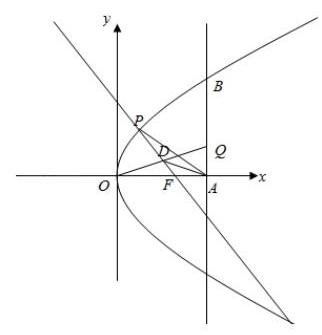
\includegraphics[max width=0.2\textwidth]{images/bo_d5jm9o77aajc7383vmi0_39_1128_229_322_335_0.jpg}
\end{center}
\hspace*{3em} 

所以 \({y}_{Q} = \frac{{16} - {y}^{2}}{8y}\left( {8 - 2}\right)  = \frac{{48} - 3{y}^{2}}{4y},Q\left( {8,\frac{{48} - 3{y}^{2}}{4y}}\right)\) ,

由 \(\overrightarrow{FP} + \overrightarrow{FQ} = \overrightarrow{FE}\) 得 \(E\left( {\frac{{y}^{2}}{8} + 6,\frac{{48} + {y}^{2}}{4y}}\right)\) ,

所以 \({\left( \frac{{48} + {y}^{2}}{4y}\right) }^{2} = 8\left( {\frac{{y}^{2}}{8} + 6}\right)\) ,解得 \({y}^{2} = \frac{16}{5}\) ,

所以存在以 \({FP}\text{ 、 }{FQ}\) 为邻边的矩形 \({FPEQ}\) ,使得点 \(E\) 在 \(\Gamma\) 上,且 \(P\left( {\frac{2}{5},\frac{4\sqrt{5}}{5}}\right) .\)

【例题】4. (2017 上海秋考) 在平面直角坐标系 \({xOy}\) 中,已知椭圆 \(\Gamma  : \frac{{x}^{2}}{4} + {y}^{2} = 1,A\) 为 \(\Gamma\) 的上顶点, \(P\) 为 \(\Gamma\) 上异于上、下顶点的动点, \(M\) 为 \(x\) 轴正半轴上的动点.

(1)若 \(P\) 在第一象限，且 \(\left| {OP}\right|  = \sqrt{2}\) ，求 \(P\) 的坐标；

(2)设 \(P\left( {\frac{8}{5},\frac{3}{5}}\right)\) ，若以 \(A\) 、 \(P\) 、 \(M\) 为顶点的三角形是直角三角形，求 \(M\) 的横坐标；

(3)若 \(\left| {MA}\right|  = \left| {MP}\right|\) ，直线 \({AQ}\) 与 \(\Gamma\) 交于另一点 \(C\) ，且 \(\overrightarrow{AQ} = 2\overrightarrow{AC}\) ， \(\overrightarrow{PQ} = 4\overrightarrow{PM}\) ，求直线 \({AQ}\) 的方程.

【解析】(1) 设 \(P\left( {x,y}\right) \left( {x > 0,y > 0}\right)\) ,因为椭圆 \(\Gamma  : \frac{{x}^{2}}{4} + {y}^{2} = 1,A\) 为 \(\Gamma\) 的上顶点,

\(P\) 为 \(\Gamma\) 上异于上、下顶点的动点, \(P\) 在第一象限,且 \(\left| {OP}\right|  = \sqrt{2}\) ,

由 \(\left\{  \begin{array}{l} \frac{{x}^{2}}{4} + {y}^{2} = 1 \\  {x}^{2} + {y}^{2} = 2 \end{array}\right.\) ,得 \(P\left( {\frac{2\sqrt{3}}{3},\frac{\sqrt{6}}{3}}\right)\) .

(2) 设 \(M\left( {{x}_{0},0}\right) ,A\left( {0,1}\right) ,P\left( {\frac{8}{5},\frac{3}{5}}\right)\) ,

若 \(\angle P = {90}^{ \circ  }\) ,则 \(\overrightarrow{PA} \cdot  \overrightarrow{PM} = 0\) ,即 \(\left( {{x}_{0} - \frac{8}{5}, - \frac{3}{5}}\right)  \cdot  \left( {-\frac{8}{5},\frac{2}{5}}\right)  = 0\) ,

所以 \(\left( {-\frac{8}{5}}\right) {x}_{0} + \frac{64}{25} - \frac{6}{25} = 0\) ,解得 \({x}_{0} = \frac{29}{20}\) .

若 \(\angle M = {90}^{ \circ  }\) ,则 \(\overrightarrow{MA} \cdot  \overrightarrow{MP} = 0\) ,即 \(\left( {-{x}_{0},1}\right)  \cdot  \left( {\frac{8}{5} - {x}_{0},\frac{3}{5}}\right)  = 0\) ,

所以 \({x}_{0}^{2} - \frac{8}{5}{x}_{0} + \frac{3}{5} = 0\) ,解得 \({x}_{0} = 1\) 或 \({x}_{0} = \frac{3}{5}\) ,

若 \(\angle A = {90}^{ \circ  }\) ,则 \(M\) 点在 \(x\) 轴负半轴,不合题意.

所以点 \(M\) 的横坐标为 \(\frac{29}{20}\) 或 1 或 \(\frac{3}{5}\) .

(3)法一:设 \(C\left( {2\cos \alpha ,\sin \alpha }\right)\) ，因为 \(\overrightarrow{AQ} = 2\overrightarrow{AC}\) ， \(A\left( {0,1}\right)\) ，

所以 \(Q\left( {4\cos \alpha ,2\sin \alpha  - 1}\right)\) ,

又设 \(P\left( {2\cos \beta ,\sin \beta }\right) ,M\left( {{x}_{0},0}\right)\) ,

因为 \(\left| {MA}\right|  = \left| {MP}\right|\) ,所以 \({x}_{0}^{2} + 1 = {\left( 2\cos \beta  - {x}_{0}\right) }^{2} + {\left( \sin \beta \right) }^{2}\) ,

整理得 \({x}_{0} = \frac{3}{4}\cos \beta\) ,

因为 \(\overrightarrow{PQ} = \left( {4\cos \alpha  - 2\cos \beta ,2\sin \alpha  - \sin \beta  - 1}\right) ,\overrightarrow{PM} = \left( {-\frac{5}{4}\cos \beta , - \sin \beta }\right)\) ,

\(\overrightarrow{PQ} = 4\overrightarrow{PM}\) ,所以 \(4\cos \alpha  - 2\cos \beta  =  - 5\cos \beta\) ,且 \(2\sin \alpha  - \sin \beta  - 1 =  - 4\sin \beta\) ,

所以 \(\cos \beta  =  - \frac{4}{3}\cos \alpha\) ,且 \(\sin \beta  = \frac{1}{3}\left( {1 - 2\sin \alpha }\right)\) ,

以上两式平方相加,整理得 \(3{\left( \sin \alpha \right) }^{2} + \sin \alpha  - 2 = 0\) ,

所以 \(\sin \alpha  = \frac{2}{3}\) 或 \(\sin \alpha  =  - 1\) (舍去),

此时直线 \({AC}\) 的斜率 \({k}_{AC} =  - \frac{1 - \sin \alpha }{2\cos \alpha } = \frac{\sqrt{5}}{10}\) (负值已舍去),

所以直线 \({AQ}\) 为 \(y = \frac{\sqrt{5}}{10}x + 1\) .

法二: 设 \(P\left( {{x}_{0},{y}_{0}}\right) ,Q\left( {{x}_{Q},{y}_{Q}}\right) ,C\left( {{x}_{C},{y}_{C}}\right) ,M\left( {m,0}\right) \left( {m > 0}\right)\) .

因为 \(P\) 为 \(\Gamma\) 上异于上、下顶点的点,所以 \(\frac{{x}_{0}^{2}}{4} + {y}_{0}^{2} = 1,{x}_{0} \neq  0\) .

由 \(\left| {MA}\right|  = \left| {MP}\right|\) ,得 \({m}^{2} + 1 = {\left( {x}_{0} - m\right) }^{2} + {y}_{0}^{2}\) ,

\({m}^{2} + 1 = {x}_{0}^{2} + {m}^{2} - {2m}{x}_{0} + \left( {1 - \frac{{x}_{0}^{2}}{4}}\right)\) ,又 \({x}_{0} \neq  0\) ,解得 \(m = \frac{3{x}_{0}}{8}\) ,

则 \(M\left( {\frac{3{x}_{0}}{8},0}\right)\) ,又 \(m > 0\) ,所以 \({x}_{0} > 0\) .

因为 \(\overrightarrow{PQ} = 4\overrightarrow{PM}\) ,所以 \(\left( {{x}_{Q} - {x}_{0},{y}_{Q} - {y}_{0}}\right)  = 4\left( {\frac{3{x}_{0}}{8} - {x}_{0}, - {y}_{0}}\right)\) ,

解得 \(\left\{  \begin{array}{l} {x}_{\theta } =  - \frac{3{x}_{0}}{2} \\  {y}_{Q} =  - 3{y}_{0} \end{array}\right.\) ,因此 \(Q\left( {-\frac{3{x}_{0}}{2}, - 3{y}_{0}}\right)\) ,

由 \(\overrightarrow{AQ} = 2\overrightarrow{AC}\) ,得 \(C\) 为 \({AQ}\) 中点,所以 \(C\left( {-\frac{3{x}_{0}}{4},\frac{1 - 3{y}_{0}}{2}}\right)\) .

因为 \(P,C\) 为椭圆上的点,所以 \(\left\{  \begin{array}{l} \frac{{x}_{0}^{2}}{4} + {y}_{0}^{2} = 1 \\  \frac{{\left( -\frac{3{x}_{0}}{4}\right) }^{2}}{4} + {\left( \frac{1 - 3{y}_{0}}{2}\right) }^{2} = 1 \end{array}\right.\) ,

解得 \(\left\{  \begin{array}{l} {x}_{0} = 0 \\  {y}_{0} = 1 \end{array}\right.\) (舍) 或 \(\left\{  \begin{array}{l} {x}_{0} = \frac{8\sqrt{5}}{9} \\  {y}_{0} =  - \frac{1}{9} \end{array}\right.\) ,则 \(Q\left( {-\frac{4\sqrt{5}}{3},\frac{1}{3}}\right)\) ,

因此直线 \({AQ}\) 的方程为 \(y = \frac{\sqrt{5}}{10}x + 1\) .

法三: 设 \(P\left( {{x}_{0},{y}_{0}}\right) ,Q\left( {{x}_{Q},{y}_{Q}}\right) ,C\left( {{x}_{C},{y}_{C}}\right) ,M\left( {m,0}\right) \left( {m > 0}\right)\) .

因为 \(\left| {MA}\right|  = \left| {MP}\right|\) ,所以 \(M\) 在 \({AP}\) 的垂直平分线上.

因为 \({AP}\) 的中点为 \(\left( {\frac{{x}_{0}}{2},\frac{{y}_{0} + 1}{2}}\right) ,{AP}\) 的斜率为 \(\frac{{y}_{0} - 1}{{x}_{0}}\) ,

所以 \({AP}\) 的垂直平分线方程为 \(y - \frac{{y}_{0} + 1}{2} =  - \frac{1}{\frac{{y}_{0} - 1}{{x}_{0}}}\left( {x - \frac{{x}_{0}}{2}}\right)\) ,

即 \(y =  - \frac{{x}_{0}}{{y}_{0} - 1}x + \frac{{x}_{0}^{2} + {y}_{0}^{2} - 1}{2\left( {{y}_{0} - 1}\right) }\) .

又 \(M\) 为 \(x\) 轴正半轴上的点,所以 \(\frac{{x}_{0}^{2} + {y}_{0}^{2} - 1}{2{x}_{0}} = \frac{{x}_{0}^{2} + \left( {1 - \frac{{x}_{0}^{2}}{4}}\right)  - 1}{2{x}_{0}} = \frac{3{x}_{0}}{8}\) ,

又 \(m > 0\) ，所以 \({x}_{0} > 0\) ，设直线 \({AQ}\) 的方程为 \(y = {kx} + 1\) .

由 \(\left\{  \begin{array}{l} \frac{{x}^{2}}{4} + {y}^{2} = 1 \\  y = {kx} + 1 \end{array}\right.\) 得 \(\left( {1 + 4{k}^{2}}\right) {x}^{2} + {8kx} = 0\) ,解得 \({x}_{C} =  - \frac{8k}{1 + 4{k}^{2}}\) ,

则 \({y}_{C} = k{x}_{C} + 1 = \frac{1 - 4{k}^{2}}{1 + 4{k}^{2}}\) ,故 \(C\) 的坐标为 \(\left( {-\frac{8k}{1 + 4{k}^{2}},\frac{1 - 4{k}^{2}}{1 + 4{k}^{2}}}\right)\) .

由 \(\overrightarrow{AQ} = 2\overrightarrow{AC}\) ,得 \(C\) 为 \({AQ}\) 中点,所以 \(Q\left( {-\frac{16k}{1 + 4{k}^{2}},\frac{1 - {12}{k}^{2}}{1 + 4{k}^{2}}}\right)\) .

因为 \(\overrightarrow{PQ} = 4\overrightarrow{PM}\) ,所以 \(\left( {-\frac{16k}{1 + 4{k}^{2}} - {x}_{0},\frac{1 - {12}{k}^{2}}{1 + 4{k}^{2}} - {y}_{0}}\right)  = 4\left( {\frac{3{x}_{0}}{8} - {x}_{0}, - {y}_{0}}\right)\) ,

解得 \(\left\{  \begin{array}{l} {x}_{0} = \frac{32k}{3\left( {1 + 4{k}^{2}}\right) } \\  {y}_{0} = \frac{1 - {12}{k}^{2}}{3\left( {1 + 4{k}^{2}}\right) } \end{array}\right.\) ,因此 \(C\left( {\frac{32k}{3\left( {1 + 4{k}^{2}}\right) },\frac{1 - {12}{k}^{2}}{3\left( {1 + 4{k}^{2}}\right) }}\right)\) .

又 \({x}_{0} > 0\) ,所以 \(k > 0\) ,因为 \(C\) 为椭圆上的点,

所以 \(\frac{{\left( \frac{32k}{3\left( {1 + 4{k}^{2}}\right) }\right) }^{2}}{4} + {\left( \frac{1 - {12}{k}^{2}}{3\left( {1 + 4{k}^{2}}\right) }\right) }^{2} = 1\) ,又 \(k > 0\) ,解得 \(k = \frac{\sqrt{5}}{10}\) ,

因此直线 \({AQ}\) 的方程为 \(y = \frac{\sqrt{5}}{10}x + 1\) . 2025 版上海高考真题及模拟训练合集(下册)

\section*{2. 模拟练习}

【练习】1. (2024 届华二) 以坐标原点为对称中心,坐标轴为对称轴的椭圆 \(\Gamma\) 过点 \(C\left( {0, - 1}\right)\) , \(D\left( {-\frac{8}{5}, - \frac{3}{5}}\right)\) .

(1)求椭圆 \(\Gamma\) 的方程和离心率.

(2)过点 \(C\left( {0, - 1}\right)\) 的直线 \(l\) 于椭圆 \(\Gamma\) 在第一象限的交点为 \(Q\) ，求三角形 \({QCD}\) 的最大面积；

(3)设 \(P\) 是椭圆上一点(异于 \(C\) 、 \(D\) )，直线 \({PC}\) 、 \({PD}\) 与 \(x\) 轴分别交于 \(M\) 、 \(N\) 两点. 在 \(x\) 轴上是否存在两点 \(A\text{ 、 }B\) ,使得 \(\overrightarrow{MB} \cdot  \overrightarrow{NA}\) 是定值？若存在,求出此定值; 若不存在,请说明理由.

【解析】(1) 不妨设椭圆方程为 \(p{x}^{2} + q{y}^{2} = 1\) ,

因为该椭圆过点 \(C\left( {0, - 1}\right) ,D\left( {-\frac{8}{5}, - \frac{3}{5}}\right)\) ,所以 \(\left\{  \begin{array}{l} q = 1 \\  \frac{64}{25}p + \frac{9}{25}q = 1 \end{array}\right.\) ,

解得 \(q = 1,p = \frac{1}{4}\) ,则椭圆的方程为 \(\frac{{x}^{2}}{4} + {y}^{2} = 1\) ;

(2) 直线 \({CD}\) 的方程为 \(x + {4y} + 4 = 0\) ,设 \(Q\left( {2\cos \theta ,\sin \theta }\right) ,\theta  \in  \left( {0,\frac{\pi }{2}}\right)\) ,

则 \(Q\) 到直线 \({CD}\) 的距离 \(d = \frac{2\cos \theta  + 4\sin \theta  + 4}{\sqrt{17}} \leq  \frac{2\sqrt{5} + 4}{\sqrt{17}}\) ,

所以三角形 \({QCD}\) 的最大面积为 \(\frac{1}{2} \times  \frac{2\sqrt{17}}{5} \times  \frac{2\sqrt{5} + 4}{\sqrt{17}} = \frac{2\sqrt{5} + 4}{5}\) ;

(3) 不妨设 \(P\left( {{x}_{0},{y}_{0}}\right) ,A\left( {m,0}\right) ,B\left( {n,0}\right)\) ,

此时直线 \({PD} : y + \frac{3}{5} = \frac{{y}_{0} + \frac{3}{5}}{{x}_{0} + \frac{8}{5}}\left( {x + \frac{8}{5}}\right)\) ,令 \(y = 0\) ,解得 \({x}_{N} = \frac{\frac{3}{5}{x}_{0} - \frac{8}{5}{y}_{0}}{{y}_{0} + \frac{3}{5}}\) ,

直线 \({PC} : y = \frac{{y}_{0} + 1}{{x}_{0}}x - 1\) ,令 \(y = 0\) ,解得 \({x}_{M} = \frac{{x}_{0}}{{y}_{0} + 1}\) ,

所以 \(\overrightarrow{MB} \cdot  \overrightarrow{NA} = \left( {n - \frac{{x}_{0}}{1 + {y}_{0}}}\right) \left( {m - \frac{\frac{3{x}_{0} - 8{y}_{0}}{5}}{{y}_{0} + \frac{3}{5}}}\right)\)

\(= \frac{\left( {n{y}_{0} + n - {x}_{0}}\right) \left( {{5m}{y}_{0} + 8{y}_{0} + {3m} - 3{x}_{0}}\right) }{\left( {1 + {y}_{0}}\right) \left( {3 + 5{y}_{0}}\right) },\)

若 \(\overrightarrow{MB} \cdot  \overrightarrow{NA}\) 是定值,不妨令 \({5m}{y}_{0} + 8{y}_{0} + {3m} =  - {3n}{y}_{0} - {3n}\) ,

因为 \({y}_{0}\) 的值不唯一,所以 \({5m} + 8 =  - {3n},{3m} =  - {3n}\) ,解得 \(m =  - 4,n = 4\) ,

则 \(\overrightarrow{MB} \cdot  \overrightarrow{NA} = \frac{-3\left\lbrack  {{\left( 4{y}_{0} + 4\right) }^{2} - {x}_{0}^{2}}\right\rbrack  }{\left( {{y}_{0} + 1}\right) \left( {5{y}_{0} + 2}\right) } = \frac{-{12}\left( {5{y}_{0}^{2} + 8{y}_{0} + 3}\right) }{5{y}_{0}^{2} + 8{y}_{0} + 3} =  - {12}\) ,

故存在 \(A\left( {-4,0}\right)\) 和 \(B\left( {4,0}\right)\) ,使得 \(\overrightarrow{MB} \cdot  \overrightarrow{NA}\) 是定值,且定值为 -12 .

【练习】2. (2025 届复附) 已知双曲线 \(C : \frac{{x}^{2}}{{a}^{2}} - \frac{{y}^{2}}{{b}^{2}} = 1\left( {a > 0,b > 0}\right)\) 的虚轴长为 4，渐近线方程为 \(y = \; \pm  {2x}\)

(1)求双曲线 \(C\) 的标准方程；

(2)设 \(A\left( {m,0}\right)\) ， \(P\) 是双曲线上的动点，求 \(\left| {PA}\right|\) 的最小值；

(3)过右焦点 \(F\) 的直线 \(l\) 与双曲线 \(C\) 的左、右两支分别交于点 \(A\) 、 \(B\) ，点 \(M\) 是线段 \({AB}\) 的中点，过点 \(F\) 且与 \(l\) 垂直的直线 \({l}^{\prime }\) 交直线 \({OM}\) 于点 \(P\) ，点 \(Q\) 满足 \(\overrightarrow{PQ} = \overrightarrow{PA} + \overrightarrow{PB}\) ，求四边形 \({PAQB}\) 面积的最小值

【解析】(1) 因为双曲线 \(C\) 的虚轴长为 4,渐近线方程为 \(y =  \pm  {2x}\) ,

所以 \(\left\{  \begin{array}{l} {2b} = 4 \\  \frac{b}{a} = 2 \end{array}\right.\) ,解得 \(a = 1,b = 2\) ,则双曲线 \(C\) 的标准方程为 \({x}^{2} - \frac{{y}^{2}}{4} = 1\) ;

(2)设 \(P\left( {x,y}\right) ,\left| {PA}\right|  = \sqrt{{\left( x - m\right) }^{2} + {y}^{2}} = \sqrt{{\left( x - m\right) }^{2} + 4{x}^{2} - 4}\)

\(= \sqrt{5{x}^{2} - {2mx} + {m}^{2} - 4}\) ,因为 \(x \leq   - 1\) 或 \(x \geq  1\) ,

当 \(\frac{m}{5} \leq   - 1\) 或 \(\frac{m}{5} \geq  1\) ,即 \(m \leq   - 5\) 或 \(m \geq  5\) 时,

\({\left| PA\right| }_{\min } = \sqrt{\frac{{20}\left( {{m}^{2} - 4}\right)  - 4{m}^{2}}{20}} = \sqrt{\frac{4{m}^{2} - {20}}{5}};\)

当 \(- 1 < \frac{m}{5} \leq  0\) ,即 \(- 5 < m \leq  0\) 时, \({\left| PA\right| }_{\min } = \left| {m + 1}\right|  =  - m - 1\) ;

当 \(0 < \frac{m}{5} < 1\) ,即 \(0 < m < 5\) 时, \({\left| PA\right| }_{\min } = \left| {m - 1}\right|\) ;

所以当 \(x = 1\) 时取得最小值 1 ;

(3) 由 (1) 得 \(F\left( {\sqrt{5},0}\right)\) ,

不妨设直线 \({AB}\) 的方程为 \(x = {my} + \sqrt{5},A\left( {{x}_{1},{y}_{1}}\right) ,B\left( {{x}_{2},{y}_{2}}\right) ,M\left( {{x}_{0},{y}_{0}}\right)\) ,

由 \(\left\{  \begin{array}{l} x = {my} + \sqrt{5} \\  4{x}^{2} - {y}^{2} = 4 \end{array}\right.\) 得 \(\left( {4{m}^{2} - 1}\right) {y}^{2} + 8\sqrt{5}{my} + {16} = 0\) ,此时 \(\Delta  = {64}\left( {{m}^{2} + 1}\right)\) ,

由韦达定理得 \({y}_{1} + {y}_{2} =  - \frac{8\sqrt{5}}{4{m}^{2} - 1}\) ,

所以 \({y}_{0} = \frac{{y}_{1} + {y}_{2}}{2} =  - \frac{4\sqrt{5}m}{4{m}^{2} - 1},{x}_{0} = m{y}_{0} + \sqrt{5} =  - \frac{\sqrt{5}}{4{m}^{2} - 1}\) ,

因为 \(O\text{ 、 }M\text{ 、 }P\) 三点共线,所以 \(\frac{{y}_{0}}{{x}_{0}} = \frac{{y}_{P}}{{x}_{P}} = {4m}\)  \circled{1} ,

因为 \({PF} \bot  {AB}\) ,所以 \({k}_{PF} \cdot  {k}_{AB} =  - 1\) ,即 \(\frac{{y}_{P} - 0}{{x}_{P} - \sqrt{5}} \cdot  \left( \frac{1}{m}\right)  =  - 1\)  \circled{2} ,

由 \circled{1}  \circled{2} 得 \(P\left( {\frac{1}{\sqrt{5}},\frac{4m}{\sqrt{5}}}\right)\) ，因为 \(\overrightarrow{PQ} = \overrightarrow{PA} + \overrightarrow{PB}\) ，

所以四边形 \({PAQB}\) 是平行四边形,此时 \({S}_{\text{ 四边形 }{PAQB}} = 2{S}_{\Delta PAB} = {d}_{P - l} \cdot  \left| {AB}\right|\) ,

因为 \({d}_{P - 1} = \frac{\left| \frac{1}{\sqrt{5}} - \frac{4{m}^{2}}{\sqrt{5}} - \sqrt{5}\right| }{\sqrt{1 + {m}^{2}}} = \frac{4}{\sqrt{5}}\sqrt{1 + {m}^{2}}\) ,

\(\left| {PQ}\right|  = \sqrt{1 + {m}^{2}} \cdot  \left| {{y}_{1} - {y}_{2}}\right|  = \sqrt{1 + {m}^{2}} \cdot  \frac{8\sqrt{{m}^{2} + 1}}{\left| 4{m}^{2} - 1\right| } = \frac{8\left( {{m}^{2} + 1}\right) }{\left| 4{m}^{2} - 1\right| },\)

所以 \({S}_{PAQB} = \frac{4}{\sqrt{5}}\sqrt{1 + {m}^{2}} \cdot  \frac{8\left( {{m}^{2} + 1}\right) }{\left| 4{m}^{2} - 1\right| } = \frac{32}{\sqrt{5}} \cdot  \frac{{\left( {m}^{2} + 1\right) }^{\frac{3}{2}}}{\left| 4{m}^{2} - 1\right| } = \frac{32}{\sqrt{5}} \cdot  \sqrt{\frac{{\left( {m}^{2} + 1\right) }^{3}}{{\left( 4{m}^{2} - 1\right) }^{2}}}\) ,

不妨令 \(t = 4{m}^{2} - 1,{m}^{2} = \frac{t + 1}{4}\) ，此时 \({S}_{PAQB} = \frac{4}{\sqrt{5}} \cdot  \sqrt{\frac{{\left( t + 5\right) }^{3}}{{t}^{2}}}\) ，

不妨令 \(f\left( t\right)  = \frac{{\left( t + 5\right) }^{3}}{{t}^{2}}\) ，函数定义域为 \(\left( {0, + \infty }\right)\) ，

得 \({f}^{\prime }\left( t\right)  = \frac{3{\left( t + 5\right) }^{2} \cdot  {t}^{2} - {2t} \cdot  {\left( t + 5\right) }^{3}}{{t}^{4}} = \frac{{\left( t + 5\right) }^{2}\left( {t - {10}}\right) }{{t}^{3}}\) ,

当 \(0 < x < {10}\) 时, \({f}^{\prime }\left( t\right)  < 0,f\left( t\right)\) 单调递减;

当 \(x > {10}\) 时, \({f}^{\prime }\left( t\right)  > 0,f\left( t\right)\) 单调递增,

所以当 \(x = {10}\) 时,函数 \(f\left( t\right)\) 取得最小值,最小值 \(f\left( {10}\right)  = \frac{135}{4}\) ,

则 \({\left( {S}_{PABQ}\right) }_{\min } = \frac{4}{\sqrt{5}} \times  \frac{3\sqrt{15}}{2} = 6\sqrt{3}\) ,

当且仅当 \(t = {10}\) ,即 \(m =  \pm  \frac{\sqrt{11}}{2}\) 时取等号

【练习】3. (2024 届建平)已知 \(A\) 、 \(B\) 分别是椭圆 \(\Gamma  : \frac{{x}^{2}}{9} + \frac{{y}^{2}}{5} = 1\) 的左、右顶点，过点 \(P\left( {0, - 3}\right)\) 、斜率为 \(k\) 的直线 \(l\) 交椭圆 \(\Gamma\) 于 \(M\) 、 \(N\) 两个不同的点.

(1)求椭圆 \(\Gamma\) 的焦距和离心率；

(2)若点 \(B\) 落在以线段 \({MN}\) 为直径的圆的外部,求 \(k\) 的取值范围；

(3)若 \(k > 0\) ，设直线 \({AM}\) 、 \({AN}\) 分别交 \(y\) 轴于点 \(S\) 、 \(T\) ， \(\overrightarrow{PS} = \lambda \overrightarrow{OP}\) ， \(\overrightarrow{PT} = \mu \overrightarrow{OP}\) ，求 \(\lambda  + \mu\) 的取值范围.

【解析】(1) 椭圆 \(\Gamma\) 的焦距为4,离心率为 \(\frac{2}{3}\) .

(2) \(B\left( {3,0}\right)\) ，设直线 \(l : y = {kx} - 3\) ，设 \(M\left( {{x}_{1},{y}_{1}}\right)\) 、 \(N\left( {{x}_{2},{y}_{2}}\right)\) ，

由 \(\left\{  \begin{matrix} y = {kx} - 3 \\  \frac{{x}^{2}}{9} + \frac{{y}^{2}}{5} = 1 \end{matrix}\right.\) 得 \(\left( {5 + 9{k}^{2}}\right) {x}^{2} - {54kx} + {36} = 0\) ,

由 \(\Delta  = {\left( {54}k\right) }^{2} - 4 \times  {36} \times  \left( {5 + 9{k}^{2}}\right)  > 0\) 解得 \(k > \frac{2}{3}\) 或 \(k <  - \frac{2}{3}\)  \circled{1} ;

因为点 \(B\left( {3,0}\right)\) 在以线段 \({MN}\) 为直径的圆的外部,所以 \(\overrightarrow{BM} \cdot  \overrightarrow{BN} > 0\) ,

又 \({x}_{1} + {x}_{2} = \frac{54k}{5 + 9{k}^{2}},{x}_{1}{x}_{2} = \frac{36}{5 + 9{k}^{2}}\) ,

\(\overrightarrow{BM} \cdot  \overrightarrow{BN} = \left( {{x}_{1} - 3,{y}_{1}}\right) \left( {{x}_{2} - 3,{y}_{2}}\right)  = \left( {1 + {k}^{2}}\right) {x}_{1}{x}_{2} - 3\left( {1 + k}\right) \left( {{x}_{1} + {x}_{2}}\right)  + {18} > 0,\)

即 \(2{k}^{2} - {9k} + 7 > 0\) ,解得 \(k < 1\) 或 \(k > \frac{7}{2}\)  \circled{2} ;

由 \circled{1}  \circled{2} 得 \(k \in  \left( {-\infty , - \frac{2}{3}}\right)  \cup  \left( {\frac{2}{3},1}\right)  \cup  \left( {\frac{7}{2}, + \infty }\right)\) .

(3) 设直线 \(l : y = {kx} - 3\) ，由 (2) 得 \(k > \frac{2}{3}\) ，记 \(M\left( {{x}_{1},{y}_{1}}\right)\) 、 \(N\left( {{x}_{2},{y}_{2}}\right)\) ，

所以直线 \({AM}\) 的方程是 \(y = \frac{{y}_{1}}{{x}_{1} + 3}\left( {x + 3}\right)\) ,

直线 \({AN}\) 的方程是 \(y = \frac{{y}_{2}}{{x}_{2} + 3}\left( {x + 3}\right)\) .

令 \(x = 0\) ,解得 \(y = \frac{3{y}_{1}}{{x}_{1} + 3}\) ,所以点 \(S\) 为 \(\left( {0,\frac{3{y}_{1}}{{x}_{1} + 3}}\right)\) ,点 \(T\) 为 \(\left( {0,\frac{3{y}_{2}}{{x}_{2} + 3}}\right)\) ,

所以 \(\overrightarrow{PS} = \left( {0,\frac{3{y}_{1}}{{x}_{1} + 3} + 3}\right) ,\overrightarrow{PT} = \left( {0,\frac{3{y}_{2}}{{x}_{2} + 3} + 3}\right) ,\overrightarrow{OP} = \left( {0, - 3}\right)\) .

由 \(\overrightarrow{PS} = \lambda \overrightarrow{OP},\overrightarrow{PT} = \mu \overrightarrow{OP}\) ,得 \(\frac{3{y}_{1}}{{x}_{1} + 3} + 3 =  - {3\lambda },\frac{3{y}_{2}}{{x}_{2} + 3} + 3 =  - {3\mu }\) ,

所以 \(\lambda  + \mu  =  - \left( {\frac{{y}_{1}}{{x}_{1} + 3} + \frac{{y}_{2}}{{x}_{2} + 3} + 2}\right)\) ,

由 (2) 得 \({x}_{1} + {x}_{2} = \frac{54k}{9{k}^{2} + 5},{x}_{1}{x}_{2} = \frac{36}{9{k}^{2} + 5}\) ,

所以 \(\lambda  + \mu  =  - \left( {\frac{k{x}_{1} - 3}{{x}_{1} + 3} + \frac{k{x}_{2} - 3}{{x}_{2} + 3} + 2}\right)\)

\(=  - \left( {\frac{{2k}{x}_{1}{x}_{2} + 3\left( {k - 1}\right) \left( {{x}_{1} + {x}_{2}}\right)  - {18}}{{x}_{1}{x}_{2} + 3\left( {{x}_{1} + {x}_{2}}\right)  + 9} + 2}\right)\)

\(=  - \left( {\frac{{2k} \cdot  \frac{36}{9{k}^{2} + 5} + 3\left( {k - 1}\right) \left( \frac{54k}{9{k}^{2} + 5}\right)  - {18}}{\frac{36}{9{k}^{2} + 5} + \left( \frac{54k}{9{k}^{2} + 5}\right)  + 9} + 2}\right)  = \frac{10}{9} \times  \frac{1}{k + 1} - 2,\) 因为 \(k > \frac{2}{3}\) ,所以 \(\frac{10}{9} \times  \frac{1}{k + 1} - 2 \in  \left( {-2, - \frac{4}{3}}\right)\) ,故 \(\lambda  + \mu\) 的范围是 \(\left( {-2, - \frac{4}{3}}\right)\) .

【练习】4. (2025 届延安) 已知点 \(A\left( {a,0}\right)\) (其中 \(a > 0\) ), \({P}_{1}\text{ 、 }{P}_{2}\text{ 、 }{P}_{3}\) 是平面直角坐标系上的三点,且 \(\left| {A{P}_{1}}\right|\) 、 \(\left| {A{P}_{2}}\right| \text{ 、 }\left| {A{P}_{3}}\right|\) 成等差数列,公差为 \(d\) .

(1) 若 \(a = 1,{P}_{1}\) 坐标为 \(\left( {1, - 1}\right) ,d = 2\) ,点 \({P}_{3}\) 在直线 \({3x} - y - {18} = 0\) 上时,求点 \({P}_{3}\) 的坐标;

(2)若 \({P}_{1}\text{ 、 }{P}_{2}\text{ 、 }{P}_{3}\) 都在抛物线 \({y}^{2} = {4x}\) 上,点 \({P}_{2}\) 的横坐标为3，且 \(a = 1\) ，求证:线段 \({P}_{1}{P}_{3}\) 的垂直平分线与 \(x\) 轴的交点为一定点,并求该定点的坐标;

(3) 若 \({P}_{1}\text{ 、 }{P}_{2}\text{ 、 }{P}_{3}\) 都在椭圆 \(\frac{{x}^{2}}{25} + \frac{{y}^{2}}{16} = 1\) ,且 \(d = 3\) ,求实数 \(a\) 的取值范围.

【解析】(1)因为 \(\left| {A{P}_{1}}\right| \text{ 、 }\left| {A{P}_{2}}\right| \text{ 、 }\left| {A{P}_{3}}\right|\) 成等差数列,且 \(\left| {A{P}_{1}}\right|  = 1,d = 2\) ,

所以 \(\left| {A{P}_{3}}\right|  = 5\) ,设 \({P}_{3}\left( {x,y}\right)\) ,

由 \(\left\{  \begin{array}{l} {\left( x - 1\right) }^{2} + {y}^{2} = {25} \\  {3x} - y - {18} = 0 \end{array}\right.\) 得 \({x}^{2} - {11x} + {30} = 0\) ,解得 \({x}_{1} = 5,{x}_{2} = 6\) ,

所以 \({P}_{3}\) 的坐标为 \(\left( {5, - 3}\right)\) 或 \(\left( {6,0}\right)\) ;

(2)因为抛物线方程为 \({y}^{2} = {4x}\) ，所以 \(A\left( {1,0}\right)\) 是它的焦点坐标，

点 \({P}_{2}\) 的横坐标为 3,即 \(\left| {A{P}_{2}}\right|  = 4\) ,设 \({P}_{1}\left( {{x}_{1},{y}_{1}}\right) ,{P}_{3}\left( {{x}_{3},{y}_{3}}\right)\) ,

则 \(\left| {A{P}_{1}}\right|  = {x}_{1} + 1,\left| {A{P}_{3}}\right|  = {x}_{3} + 1,\left| {A{P}_{1}}\right|  + \left| {A{P}_{3}}\right|  = 2\left| {A{P}_{2}}\right|\) ,

所以 \({x}_{1} + {x}_{3} = 2{x}_{2} = 6\) ,

直线 \({P}_{1}{P}_{3}\) 的斜率 \(k = \frac{{y}_{3} - {y}_{1}}{{x}_{3} - {x}_{1}} = \frac{4}{{y}_{3} + {y}_{1}}\) ,

则线段 \({P}_{1}{P}_{3}\) 的垂直平分线 \(l\) 的斜率 \({k}_{l} =  - \frac{{y}_{3} + {y}_{1}}{4}\) ,

则线段 \({P}_{1}{P}_{3}\) 的垂直平分线 \(l\) 的方程为 \(y - \frac{{y}_{3} + {y}_{1}}{2} =  - \frac{{y}_{3} + {y}_{1}}{4}\left( {x - 3}\right)\) ,

直线 \(l\) 与 \(x\) 轴的交点为定点 \(\left( {5,0}\right)\) ;

(3) 设 \(P\left( {x,y}\right)\) 是椭圆 \(\frac{{x}^{2}}{25} + \frac{{y}^{2}}{16} = 1\) 上一点,则 \({y}^{2} = {16}\left( {1 - \frac{{x}^{2}}{25}}\right) , - 5 \leq  x \leq  5\) .

已知 \(A\left( {a,0}\right) \left( {a > 0}\right) ,\left| {AP}\right|  = \sqrt{{\left( x - a\right) }^{2} + {y}^{2}} = \sqrt{{\left( x - a\right) }^{2} + {16}\left( {1 - \frac{{x}^{2}}{25}}\right) }\)

\(\left| {AP}\right|  = \sqrt{{\left( x - a\right) }^{2} + {y}^{2}} = \sqrt{{\left( x - a\right) }^{2} + {16}\left( {1 - \frac{{x}^{2}}{25}}\right) } = \sqrt{{x}^{2} - {2ax} + {a}^{2} + {16} - \frac{{16}{x}^{2}}{25}} = ,\)

令 \(f\left( x\right)  = \frac{9{x}^{2}}{25} - {2ax} + {a}^{2} + {16},x \in  \left\lbrack  {-5,5}\right\rbrack\) ,其对称轴为 \(x = \frac{25a}{9}\) .

因为 \(\left| {A{P}_{1}}\right| ,\left| {A{P}_{2}}\right| ,\left| {A{P}_{3}}\right|\) 成等差数列,公差 \(d = 3\) ,

所以 \(\left| {AP}\right|\) 的最大值与最小值之差不小于 6 .

 \circled{1}  当 \(0 < \frac{25a}{9} \leq  5\) ，即 \(0 < a \leq  \frac{9}{5}\) 时，

\(f{\left( x\right) }_{\min } = f\left( \frac{25a}{9}\right)  = {a}^{2} + {16} - \frac{{25}{a}^{2}}{9} = {16} - \frac{{16}{a}^{2}}{9},\)

\(f{\left( x\right) }_{\max } = f\left( {-5}\right)  = 9 + {10a} + {a}^{2} + {16} = {a}^{2} + {10a} + {25},\)

所以 \(\sqrt{{a}^{2} + {10a} + {25}} - \sqrt{{16} - \frac{{16}{a}^{2}}{9}} \geq  6\) ,所以 \(a + 5 - \sqrt{{16} - \frac{{16}{a}^{2}}{9}} \geq  6\) ,

所以 \(a - 1 \geq  \sqrt{{16} - \frac{{16}{a}^{2}}{9}}\) ,则有 \(a \geq  1\) ,

解得 \(a \leq  \frac{9 - {24}\sqrt{6}}{25}\) 或 \(a \geq  \frac{9 + {24}\sqrt{6}}{25}\) ,都不符合 \(0 < a \leq  \frac{9}{5}\) ,均舍去;

 \circled{2}  当 \(\frac{25a}{9} > 5\) ，即 \(a > \frac{9}{5}\) 时，

\(f{\left( x\right) }_{\min } = f\left( 5\right)  = 9 - {10a} + {a}^{2} + {16} = {a}^{2} - {10a} + {25},\)

\(f{\left( x\right) }_{\max } = f\left( {-5}\right)  = {a}^{2} + {10a} + {25},\)

所以 \(\sqrt{{a}^{2} + {10a} + {25}} - \sqrt{{a}^{2} - {10a} + {25}} \geq  6\) ,所以 \(a + 5 - \left| {a - 5}\right|  \geq  6\) ,

结合 \(a > \frac{9}{5}\) ,得 \(a \geq  3\) .

综上,实数 \(a\) 的取值范围是 \(\lbrack 3, + \infty )\) .

【练习】5. (未来星教研) 已知椭圆 \(\Gamma  : \frac{{x}^{2}}{2} + {y}^{2} = 1\) 的右焦点为 \(F\left( {{x}_{F},{y}_{F}}\right) ,P\left( {{x}_{P},{y}_{P}}\right)\) 为 \(\Gamma\) 上一点,过 \(P\) 的直线 \(l\) 交动直线 \(y = m\left( {m > 0}\right)\) 于 \(M\left( {{x}_{M},m}\right)\) .

(1)当 \(m = 4\) 且 \({y}_{P} = 1\) 时， \(l\) 经过 \(F\) ，求 \(M\) 的坐标；

(2)已知 \({x}_{F} = {x}_{P}\) ，设直线 \(y = m\) 交 \(y\) 轴于 \(Q\) ，若 \(l\) 的倾斜角为 \(\frac{\pi }{3}\) 且 \(\bigtriangleup  {PMQ}\) 为等腰三角形，求 \(m\) 的值;

(3) 已知 \(m = 6\) ，若对任意的 \(P\) ， \(F\) 到 \(l\) 的距离始终为 \(\sqrt{2}\) ，求 \({x}_{M}\) 的最大值.

【解析】(1)因为 \({y}_{P} = 1\) ,故 \({x}_{P} = 0\) ; 且 \(F\) 的坐标为 \(\left( {1,0}\right)\)

所以可得直线 \({PF}\) 方程为: \(y =  - x + 1,2\) 分

代入 \(y = 4\) ，可得 \({x}_{M} =  - 3\) ，故 \(M\) 的坐标为 \(\left( {-3,4}\right)\)

(2) 当 \({x}_{P} = {x}_{F}\) 时,可解得: \({y}_{P} =  \pm  \frac{\sqrt{2}}{2}\)

情况 \circled{1} :当 \({y}_{P} = \frac{\sqrt{2}}{2}\) 且 \(m \in  \left( {1, + \infty }\right)\) ，根据几何关系可得:

\begin{center}
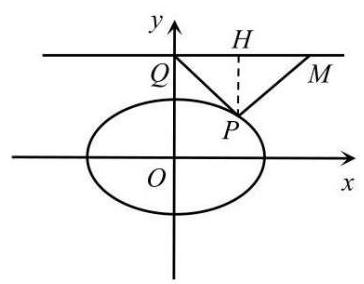
\includegraphics[max width=0.3\textwidth]{images/bo_d5jm9o77aajc7383vmi0_46_1085_1274_364_284_0.jpg}
\end{center}
\hspace*{3em} 

\(\angle {PMQ} = {60}^{ \circ  }\) ,

从而可得: \(\bigtriangleup {PMQ}\) 是等边三角形,因此可得: \({QH} = {HM} = 1\) ,可得方程: \(\tan \frac{\pi }{3} = m - \frac{\sqrt{2}}{2}\) ,

解得: \(m = \sqrt{3} + \frac{\sqrt{2}}{2}\)

情况 \circled{2} :当 \({y}_{P} = \frac{\sqrt{2}}{2}\) 且 \(m \in  (0,1\rbrack\) ，可得: \(\angle {PMQ} > {90}^{ \circ  }\) ，当

\({\Delta PMQ}\) 是等腰三角形，

只有 \({PM} = {MQ}\) 成立，根据几何关系可得: \({\angle {PMQ}} = {120}^{ \circ  }\) ，从而 \({\angle {PQM}} = {30}^{ \circ  }\) ，

可得方程: \(\tan \frac{\pi }{6} = \frac{\sqrt{2}}{2} - m\) ,解得: \(m = \frac{\sqrt{2}}{2} - \frac{\sqrt{3}}{3}\) , 2025 版上海高考真题及模拟训练合集(下册)

\begin{center}
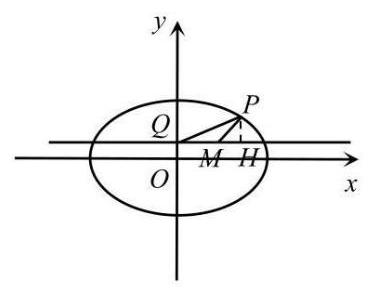
\includegraphics[max width=0.3\textwidth]{images/bo_d5jm9o77aajc7383vmi0_46_304_1772_368_290_0.jpg}
\end{center}
\hspace*{3em} 

情况 \circled{3} :当 \({y}_{P} =  - \frac{\sqrt{2}}{2}\) 且 \(m \in  \left( {0, + \infty }\right)\) ，同情况 \circled{1} 解得: \(m = \sqrt{3} - \frac{\sqrt{2}}{2}\)

\begin{center}
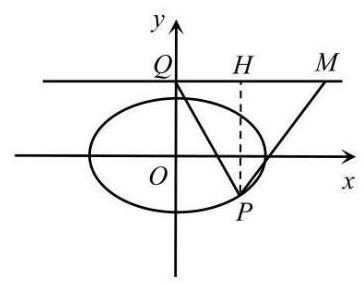
\includegraphics[max width=0.3\textwidth]{images/bo_d5jm9o77aajc7383vmi0_47_307_315_364_285_0.jpg}
\end{center}
\hspace*{3em} 

综上, \(m = \frac{\sqrt{2}}{2} - \frac{\sqrt{3}}{3}\) 或 \(m = \sqrt{3} \pm  \frac{\sqrt{2}}{2}\) .

(3) \circled{1} 当直线 \(l\) 的斜率不存在时，直线 \(l\) 方程: \(x = 1 - \sqrt{2}\) ， \({x}_{M} = 1 - \sqrt{2}\) ，

 \circled{2} 当直线 \(l\) 的斜率存在时,由于与直线 \(y = 6\) 有交点，则斜率不为 0 ，

设直线 \(l\) 方程: \(y = {kx} + b\left( {k \neq  0}\right)\) ，又因为 \(F\) 到 \(l\) 的距离为 \(\sqrt{2}\) ，

故 \(l\) 始终与圆 \(\left( {x - 1}\right)  + {y}^{2} = 2\) 相切,设切点为 \(N\)

因为 \(\left\{  \begin{array}{l} y = {kx} + b \\  {\left( x - 1\right) }^{2} + {y}^{2} = 2 \end{array}\right.\) ,可得: \(\left( {1 + {k}^{2}}\right) {x}^{2} + \left( {{2kb} - 2}\right) x + {b}^{2} - 1 = 0\) ,

进而可得: \(\Delta  = {k}^{2} - {b}^{2} - {2kb} + 2 = 0\)

同理 \(\left\{  \begin{array}{l} y = {kx} + b \\  \frac{{x}^{2}}{2} + {y}^{2} = 1 \end{array}\right.\) ,可得: \(\left( {1 + 2{k}^{2}}\right) {x}^{2} + {4kbx} + 2{b}^{2} - 2 = 0\) ,

\begin{center}
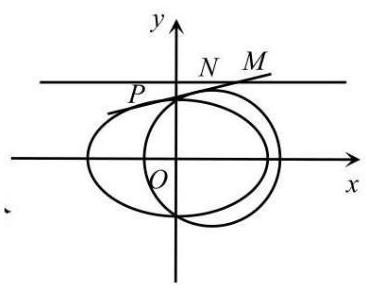
\includegraphics[max width=0.3\textwidth]{images/bo_d5jm9o77aajc7383vmi0_47_1092_1124_367_290_0.jpg}
\end{center}
\hspace*{3em} 

进而可得: \(\Delta  = {16}{k}^{2} - 8{b}^{2} + 8 \geq  0\)

又因为当 \(m = 6\) 时, \({x}_{M} = \frac{6 - b}{k}\) ,

又因为: \(\left\{  \begin{array}{l} {k}^{2} - {b}^{2} - {2kb} + 2 = 0 \\  2{k}^{2} - {b}^{2} + 1 \geq  0 \end{array}\right.\) ,

显然: 当 \({x}_{M}\) 为最大值时,有且仅有 \({16}{k}^{2} - 8{b}^{2} + 8 = 0\) 成立 (情况如图所示),

解得: \(k = \frac{\sqrt{7}}{7},b = \frac{3\sqrt{7}}{7}\) (增根已舍),

代入可得: \({x}_{M} = 6\sqrt{7} - 3 > 1 - \sqrt{2}\) ,

综上所述， \({x}_{M}\) 的最大值为 \(6\sqrt{7} - 3\)

【练习】6. 已知抛物线 \(G : {y}^{2} = {8x}\) 的焦点与椭圆 \(E : \frac{{x}^{2}}{5} + {y}^{2} = 1\) 的右焦点 \(F\) 重合,过点 \(F\) 且斜率为 \(k\) 的直线 \(l\) 交椭圆 \(E\) 于 \(A\) 、 \(B\) 两点,交抛物线 \(G\) 于 \(M\) 、 \(N\) 两点,请问是否存在实常数 \(m\) ,使 \(\frac{\sqrt{5}}{\left| AB\right| } + \frac{m}{\left| MN\right| }\) 为定值? 若存在,求出 \(m\) 的值; 若不存在,说明理由.

\begin{center}
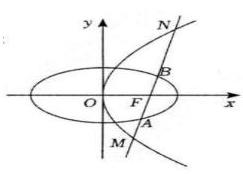
\includegraphics[max width=0.2\textwidth]{images/bo_d5jm9o77aajc7383vmi0_47_1218_1661_243_174_0.jpg}
\end{center}
\hspace*{3em} 

【解析】法一: 设 \(A\left( {{x}_{1},{y}_{1}}\right) \text{ 、 }B\left( {{x}_{2},{y}_{2}}\right) \text{ 、 }M\left( {{x}_{3},{y}_{3}}\right) \text{ 、 }N\left( {{x}_{4},{y}_{4}}\right)\) ,

直线 \(l\) 的方程 \(y = k\left( {x - 2}\right)\) ,由 \(\left\{  \begin{array}{l} \frac{{x}^{2}}{5} + {y}^{2} = 1 \\  y = k\left( {x - 2}\right)  \end{array}\right.\) 得 \(\left( {1 + 5{k}^{2}}\right) {x}^{2} - {20}{k}^{2}x + {20}{k}^{2} - 5 = 0\) ,

所以 \({x}_{1} + {x}_{2} = \frac{{20}{k}^{2}}{1 + 5{k}^{2}},{x}_{1}{x}_{2} = \frac{{20}{k}^{2} - 5}{1 + 5{k}^{2}}\) ,

所以 \(\left| {AB}\right|  = \sqrt{1 + {k}^{2}} \cdot  \sqrt{{\left( {x}_{1} + {x}_{2}\right) }^{2} - 4{x}_{1}{x}_{2}} = \frac{2\sqrt{5}\left( {{k}^{2} + 1}\right) }{1 + 5{k}^{2}}\) ,

由 \(\left\{  \begin{array}{l} {y}^{2} = 8 \\  y = k\left( {x - 2}\right)  \end{array}\right.\) ,得 \({k}^{2}{x}^{2} - \left( {4{k}^{2} + 8}\right) x + 4{k}^{2} = 0\) ,

所以 \({x}_{3} + {x}_{4} = \frac{4{k}^{2} + 8}{{k}^{2}},{x}_{3}{x}_{4} = 4\) ,所以 \(\left| {MN}\right|  = {x}_{3} + {x}_{4} + 4 = \frac{8\left( {{k}^{2} + 1}\right) }{{k}^{2}}\) ,

所以 \(\frac{\sqrt{5}}{\left| AB\right| } + \frac{m}{\left| MN\right| } = \frac{1 + 5{k}^{2}}{2\left( {{k}^{2} + 1}\right) } + \frac{m{k}^{2}}{8\left( {{k}^{2} + 1}\right) } = \frac{\left( {{20} + m}\right) {k}^{2} + 4}{8\left( {{k}^{2} + 1}\right) }\) ,

要使 \(\frac{\sqrt{5}}{\left| AB\right| } + \frac{1}{\left| MN\right| }\) 为常数,则 \({20} + m = 4\) ,解得 \(m =  - {16}\) ,

故存在 \(m =  - {16}\) ，使得 \(\frac{\sqrt{5}}{\left| AB\right| } + \frac{1}{\left| MN\right| }\) 为定值 \(\frac{1}{2}\) .

法二:直线的参数方程

设直线 \(l\) 的方程 \(\left\{  \begin{array}{l} x = 2 + t\cos \alpha \\  y = t\sin \alpha  \end{array}\right.\)

联立直线 \(l\) 与抛物线 \(G\) ,得 \({\sin }^{2}\alpha {t}^{2} - 8\cos {\alpha t} - {16} = 0\)

所以 \(\left| {MN}\right|  = \left| {{t}_{1} - {t}_{2}}\right|  = \frac{8}{{\sin }^{2}\alpha }\)

联立直线 \(l\) 与椭圆 \(E\) ,得 \(\left( {4{\sin }^{2}\alpha  + 1}\right) {t}^{2} + 4\cos {\alpha t} - 1 = 0\)

所以 \(\left| {AB}\right|  = \left| {{t}_{3} - {t}_{4}}\right|  = \frac{2\sqrt{5}}{4{\sin }^{2}\alpha  + 1}\)

所以 \(\frac{\sqrt{5}}{\left| AB\right| } + \frac{m}{\left| MN\right| } = \frac{4{\sin }^{2}\alpha  + 1}{2} + \frac{m}{8}{\sin }^{2}\alpha  = \left( {2 + \frac{m}{8}}\right) {\sin }^{2}\alpha  + \frac{1}{2}\)

故存在 \(m =  - {16}\) ,使得 \(\frac{\sqrt{5}}{\left| AB\right| } + \frac{1}{\left| MN\right| }\) 为定值 \(\frac{1}{2}\) .

【练习】7. (23 奉贤一模) 已知椭圆 \(C\) 的中心在原点 \(O\) ，且它的一个焦点 \(F\) 为 \(\left( {\sqrt{3},0}\right)\) . 点 \({A}_{1}\) ， \({A}_{2}\) 分别是椭圆的左、右顶点,点 \(B\) 为椭圆的上顶点, \({\Delta OFB}\) 的面积为 \(\frac{\sqrt{3}}{2}\) . 点 \(M\) 是椭圆 \(C\) 上在第一象限内的一个动点.

(1)求椭圆 \(C\) 的标准方程；

(2)若把直线 \(M{A}_{1},M{A}_{2}\) 的斜率分别记作 \({k}_{1},{k}_{2}\) ,若 \({k}_{1} + {k}_{2} =  - \frac{3}{4}\) ,求点 \(M\) 的坐标;

(3)设直线 \(M{A}_{1}\) 与 \(y\) 轴交于点 \(P\) ，直线 \(M{A}_{2}\) 与 \(y\) 轴交于点 \(Q\) . 令 \(\overrightarrow{PB} = \lambda \overrightarrow{BQ}\) ，求实数 \(\lambda\) 的取值范围.

【答案】 \(\left( 1\right) \frac{{x}^{2}}{4} + \frac{{y}^{2}}{1} = 1;\left( 2\right) M\left( {\frac{6}{5},\frac{4}{5}}\right) ;\left( 3\right) \lambda  \in  \left( {0,1}\right)\)

【解析】(1) 由题意得 \(\left\{  \begin{array}{l} {a}^{2} - {b}^{2} = 3 \\  \frac{1}{2}{bc} = \frac{\sqrt{3}}{2} \\  c = \sqrt{3} \end{array}\right.\) ,所以 \(\left\{  \begin{array}{l} a = 2 \\  b = 1 \end{array}\right.\) ,所以椭圆标准方程为 \(\frac{{x}^{2}}{4} + \frac{{y}^{2}}{1} = 1\)

(2) 设 \(M\left( {{x}_{0},{y}_{0}}\right) ,{A}_{1}\left( {-2,0}\right) ,{A}_{2}\left( {2,0}\right)\) .

\(\left\{  \begin{array}{l} \frac{{x}_{0}^{2}}{4} + \frac{{y}_{0}^{2}}{1} = 1 \\  \frac{{y}_{0}}{{x}_{0} + 2} + \frac{{y}_{0}}{{x}_{0} - 2} =  - \frac{3}{4}\text{ ,得 }{y}_{0} = \frac{3\left( {4 - {x}_{0}^{2}}\right) }{8{x}_{0}}\text{ ,解得 }M\left( {\frac{6}{5},\frac{4}{5}}\right) \\  {x}_{0} > 0,{y}_{0} > 0 \end{array}\right.\)

(3)法一:直线 \(M{A}_{1}\) 的方程为 \(y = {k}_{1}\left( {x + 2}\right)\) ，所以 \(P\left( {0,2{k}_{1}}\right)\)

直线 \(M{A}_{2}\) 的方程为 \(y = {k}_{2}\left( {x - 2}\right)\) ,所以 \(P\left( {0, - 2{k}_{2}}\right)\) ,

\(\overrightarrow{PB} = \left( {0,1 - 2{k}_{1}}\right) ,\overrightarrow{BQ} = \left( {0, - 2{k}_{2} - 1}\right) ,\)

所以 \(\lambda  = \frac{1 - 2{k}_{1}}{-2{k}_{2} - 1}\) ,

因为 \({k}_{1}{k}_{2} = \frac{{y}_{0}}{{x}_{0} + 2} \cdot  \frac{{y}_{0}}{{x}_{0} - 2} = \frac{{y}_{0}^{2}}{{x}_{0}^{2} - 4} =  - \frac{1}{4}\)

所以 \(\lambda  = \frac{1 - 2{k}_{1}}{-2\frac{1}{-4{k}_{1}} - 1} = 2{k}_{1}\)

因为 \({k}_{1} = \frac{{y}_{0}}{{x}_{0} + 2} = \frac{\sqrt{1 - \frac{{x}_{0}^{2}}{4}}}{{x}_{0} + 2} = \frac{1}{2}\sqrt{\frac{2 - {x}_{0}}{2 + {x}_{0}}} = \frac{1}{2}\sqrt{\frac{4}{2 + {x}_{0}} - 1},{x}_{0} \in  \left( {0,2}\right)\) ,

所以 \({k}_{1} \in  \left( {0,\frac{1}{2}}\right)\) ,所以 \(\lambda  \in  \left( {0,1}\right)\)

法二: (参数方程) 设 \(M\left( {2\cos \theta ,\sin \theta }\right)\) ,其中 \(\theta  \in  \left( {0,\frac{\pi }{2}}\right) ,{A}_{1}\left( {-2,0}\right) ,{A}_{2}\left( {2,0}\right)\) ,

则 \(P\left( {0,\frac{\sin \theta }{\cos \theta  + 1}}\right)\) ,即 \(P\left( {0,\tan \frac{\theta }{2}}\right) ,Q\left( {0,\frac{1}{\tan \frac{\theta }{2}}}\right)\)

\(\lambda  = \frac{1 - \tan \frac{\theta }{2}}{\frac{1}{\tan \frac{\theta }{2}} - 1} = \tan \frac{\theta }{2} \in  \left( {0,1}\right)\)

【练习】8. (艺扬飞翔) 已知点 \(F\) 是抛物线 \({y}^{2} = {4x}\) 的焦点，动点 \(P\) 在抛物线上，设直线 \(l\) 与抛物线交于 \(D\text{ 、 }E\) 两点 \(\left( {P\text{ 、 }D\text{ 、 }E\text{ 均不重合 }}\right)\) .)

(1) 若 \(l\) 经过点 \(F,\left| {DF}\right|  = 3\) ，求 \(E\) 点坐标；

(2)若 \(\overrightarrow{DF} = \overrightarrow{PE}\) ，证明:直线 \({DE}\) 过定点；

(3)若 \(\angle {DPF} = \angle {DEF}\) 且 \(\angle {EDP} = \angle {EFP}\) ,四边形 \({DPFE}\) 面积为 \(\sqrt{2}\) ，求直线 \(l\) 的方程.

\begin{center}
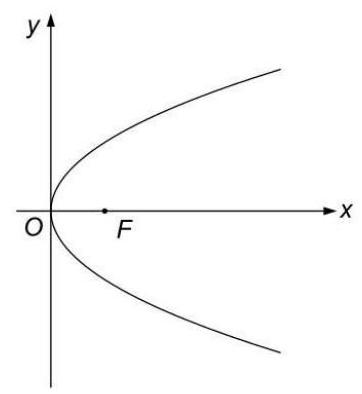
\includegraphics[max width=0.3\textwidth]{images/bo_d5jm9o77aajc7383vmi0_49_301_1337_362_394_0.jpg}
\end{center}
\hspace*{3em} 

【解析】(1) 由抛物线的几何意义, \(D\left( {2, \pm  2\sqrt{2}}\right)\) 时:

设 \(E\left( {{b}^{2},{2b}}\right)\) ,当 \(D\) 在 \(\left( {2,2\sqrt{2}}\right)\) 时:

\({DE}\) 方程: \(x = \frac{b + \sqrt{2}}{2}y - \sqrt{2}b\) ,解得 \(b =  - \frac{1}{\sqrt{2}}\) ,即 \(E\left( {\frac{1}{2}, - \sqrt{2}}\right)\)

同理, \(D\left( {2, - 2\sqrt{2}}\right)\) ,解得 \(E\left( {\frac{1}{2},\sqrt{2}}\right)\) ,故 \(E\) 点坐标为 \(\left( {\frac{1}{2}, \pm  \sqrt{2}}\right)\)

(2) 设 \(D\left( {{a}^{2},{2a}}\right)\) ， \(E\left( {{b}^{2},{2b}}\right)\) ， \(P\left( {{p}^{2},{2p}}\right)\) ， \(\left\{  \begin{array}{l} {b}^{2} - {p}^{2} = 1 - {a}^{2} \\  {2b} - {2p} =  - {2a} \end{array}\right.\) ，化简得 \(\left\{  \begin{matrix} {a}^{2} + {b}^{2} = 1 + {p}^{2} \\  a + b = p \end{matrix}\right.\) 解得 \({2ab} =\)

\begin{center}
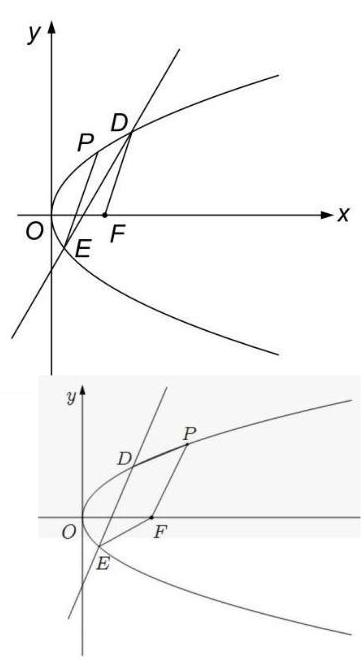
\includegraphics[max width=0.3\textwidth]{images/bo_d5jm9o77aajc7383vmi0_50_1090_236_364_670_0.jpg}
\end{center}
\hspace*{3em} 

\({\left( a + b\right) }^{2} - \left( {{a}^{2} + {b}^{2}}\right)  =  - 1,{ab} =  - \frac{1}{2}\) 而 \({DE}\) 方程: \(x = \frac{b + a}{2}y - \; {ab}\) ,故过定点 \(\left( {\frac{1}{2},0}\right)\)

(3) 设 \(D\left( {{a}^{2},{2a}}\right) ,E\left( {{b}^{2},{2b}}\right) ,P\left( {{p}^{2},{2p}}\right)\) ,由题,四边形 \({DPFE}\) 为平行四边形.

\(\left\{  {\begin{matrix} {a}^{2} - {b}^{2} = {p}^{2} - 1 \\  {2a} - {2b} = {2p} \end{matrix}\text{ ,解得 }\left\{  \begin{matrix} a = p - \frac{1}{2p} \\  b =  - \frac{1}{2p} \end{matrix}\right. }\right.\)

\({S}_{DPFE} = 2{S}_{\bigtriangleup {DFE}} = 2 \cdot  \frac{1}{2} \cdot  \left| {\left( {{y}_{D} - {y}_{E}}\right) \left( {1 + {ab}}\right) }\right|\)

\(\therefore {S}_{DPFE} = \left| {p + \frac{1}{2p}}\right|  = \sqrt{2},p =  \pm  \frac{\sqrt{2}}{2}\)

\(\therefore {DE}\) 方程: \(x = \frac{b + a}{2}y - {ab}\) ,解得 \(l : y =  \pm  2\sqrt{2}x\) .

【练习】9. (年少有为) 已知抛物线 \(\Gamma  : {y}^{2} = {4x}\) ，焦点为 \(F\) ， \(P\) 为 \(x\) 轴负半轴上一点，过 \(P\) 作直线 \(l\) 分别交 \(\Gamma\) 于 \(A\) 、 \(B\) 不同两点，满足 \(A\) 、 \(B\) 均在 \(x\) 轴上方，且 \(B\) 在线段 \({AP}\) 上.

(1)若直线 \(l\) 的斜率为 \(\frac{1}{2}\) ，且 \({BF} \bot  {PF}\) ，求 \(P\) 点坐标；

(2)是否存在直线 \(l\) ，使得 \(\left| {BF}\right|  = \frac{3}{2}\) ， \(\left| {AF}\right|  = 5\) ， \({FA}\bot {FB}\) ？若存在，求出直线 \(l\) 的方程；若不存在, 说明理由;

(3) 若存在直线 \(l\) 与 \(x\) 轴上一点 \(Q\) ,使得四边形 \({ABFQ}\) 为等腰梯形,求 \(P\) 点横坐标的取值范围.

【解析】 \(\left( 1\right) F\left( {1,0}\right)\) . 因为 \({BF} \bot  {PF}\) ,故 \({x}_{B} = {x}_{F} = 1\) ,而 \(B\) 在抛物线上,故 \(B\left( {1,2}\right)\) . 因为直线 \(l\) 的斜率为 \(\frac{1}{2}\) ,故直线 \(1 : y - 2 = \frac{1}{2}\left( {x - 1}\right)\) . 令 \(y = 0\) ,解得 \(x =  - 3,P\left( {-3,0}\right)\) .

(2)假设这样的直线 \(l\) 存在. 由抛物线定义， \(\left| {BF}\right|  = {x}_{B} + 1 = \frac{3}{2}\) ，故 \({x}_{B} = \frac{1}{2}\) ， \(B\left( {\frac{1}{2},\sqrt{2}}\right)\) . \(\left| {AF}\right| \; = {x}_{A} + 1 = 5\) ,故 \({x}_{A} = 4,A\left( {4,4}\right) .\overrightarrow{FB} = \left( {-\frac{1}{2},\sqrt{2}}\right) ,\overrightarrow{FA} = \left( {3,4}\right)\) ,故 \(\overrightarrow{FB} \cdot  \overrightarrow{FA} =  - \frac{3}{2} + 4\sqrt{2} \neq  0\) , 于是 \({FA}\) 与 \({FB}\) 不垂直,矛盾! 故假设不成立,这样的直线 \(l\) 不存在.

(3) 设 \(P\left( {m,0}\right)\) ,则 \(m < 0\) . 设 \(A\left( {{a}^{2},{2a}}\right) ,B\left( {{b}^{2},{2b}}\right)\) ,则 \(a > b > 0\) .

直线 \({AB} : {2x} - \left( {a + b}\right) y + {2ab} = 0\) ,将 \(P\left( {m,0}\right)\) 坐标代入得 \({ab} =  - m\) .

因为 \({ABFQ}\) 为等腰梯形,且 \({AB}\) 与 \({FQ}\) 不平行,故 \({BF}//{AQ}\) ,从而 \(\angle {PBF} = \angle {PFB},{PB} = {PF}\) .

反之,当 \({PB} = {PF}\) 时,延长 \({PF}\) 至点 \(Q\) ,使得 \({FQ} = {BA}\) .

因为 \(\frac{PB}{BA} = \frac{PF}{FQ}\) ,故 \({BF}//{AQ}\) ,从而此时 \({ABFQ}\) 为等腰梯形.

因此,题设等价于 \({PB} = {PF}\) .

\(1 - m = \sqrt{{\left( {b}^{2} - m\right) }^{2} + 4{b}^{2}}\) ,平方得 \({b}^{4} + \left( {4 - {2m}}\right) {b}^{2} + \left( {{2m} - 1}\right)  = 0\) ,其中 \(0 < {b}^{2} <  - m\) . (因为 \(\left. {-m = {ab} > {b}^{2}}\right)\)

记 \({b}^{2} = t\) ,则关于 \(t\) 的方程 \({t}^{2} + \left( {4 - {2m}}\right) t + \left( {{2m} - 1}\right)  = 0\) 有属于 \(\left( {0, - m}\right)\) 的解.

记 \(f\left( t\right)  = {t}^{2} + \left( {4 - {2m}}\right) t + \left( {{2m} - 1}\right)\) . 因为 \(y = f\left( t\right)\) 的图像关于直线 \(x = m - 2\) 成轴对称,

\(m - 2 < 0\) ,故 \(f\left( t\right)\) 在区间 \(\left( {0, - m}\right)\) 上严格增,从而 \(\left\{  \begin{array}{l} f\left( 0\right)  < 0 \\  f\left( {-m}\right)  > 0 \end{array}\right.\) , \(\left\{  \begin{array}{l} {2m} - 1 < 0 \\  3{m}^{2} - {2m} - 1 > 0 \end{array}\right.\) ,

\(\left\{  \begin{array}{l} m < \frac{1}{2} \\  m <  - \frac{1}{3}\text{ 或 }m > 1 \end{array}\right.\) ,解得 \(m <  - \frac{1}{3}\) ,即为所求.

【练习】10. (2024 届复兴) 已知直线 \(l\) 与抛物线 \({C}_{1} : {y}^{2} = {2x}\) 交于两点 \(A\left( {{x}_{1},{y}_{1}}\right) ,B\left( {{x}_{2},{y}_{2}}\right)\) ,与抛物线 \({C}_{2}\) : \({y}^{2} = {4x}\) 交于两点 \(C\left( {{x}_{3},{y}_{3}}\right) ,D\left( {{x}_{4},{y}_{4}}\right)\) ,其中 \(A\text{ 、 }C\) 在第一象限, \(B\text{ 、 }D\) 在第四象限.

(1)若直线 \(l\) 过点 \(M\left( {1,0}\right)\) ，且 \(\frac{1}{\left| BM\right| } - \frac{1}{\left| AM\right| } = \frac{\sqrt{2}}{2}\) ，求直线 \(l\) 的方程；

(2)求证: \(\frac{1}{{y}_{1}} + \frac{1}{{y}_{2}} = \frac{1}{{y}_{3}} + \frac{1}{{y}_{4}}\) ;

(3)设 \(\bigtriangleup  {AOB}\text{ 、 } \bigtriangleup  {COD}\) 的面积分别为 \({S}_{1}\) 、 \({S}_{2}\) ( \(O\) 为坐标原点)，若 \(\left| {AC}\right|  = 2\left| {BD}\right|\) ，求 \(\frac{{S}_{1}}{{S}_{2}}\) 的值.

【解析】(1) 显然直线 \(l\) 的斜率不为 0,设直线 \(l\) 的方程为 \(x = {my} + 1\) ,

由 \(\left\{  \begin{array}{l} x = {my} + 1 \\  {y}^{2} = {2x} \end{array}\right.\) 得 \({y}^{2} - {2my} - 2 = 0\) ,

得 \({y}_{1} + {y}_{2} = {2m},{y}_{1}{y}_{2} =  - 2\) ,则 \(\frac{{y}_{1} + {y}_{2}}{{y}_{1}{y}_{2}} =  - m\) ,

则 \(\frac{1}{\left| BM\right| } - \frac{1}{\left| AM\right| } =  - \frac{1}{\sqrt{1 + {m}^{2}}{y}_{2}} - \frac{1}{\sqrt{1 + {m}^{2}} \cdot  {y}_{1}} =  - \frac{1}{\sqrt{1 + {m}^{2}}} \cdot  \left( {\frac{1}{{y}_{2}} + \frac{1}{{y}_{1}}}\right)\)

\(=  - \frac{1}{\sqrt{1 + {m}^{2}}} \cdot  \frac{{y}_{1} + {y}_{2}}{{y}_{1}{y}_{2}} =  - \frac{1}{\sqrt{1 + {m}^{2}}} \cdot  \left( {-m}\right)  = \frac{m}{\sqrt{1 + {m}^{2}}}\) ,

由题意得 \(\frac{m}{\sqrt{1 + {m}^{2}}} = \frac{\sqrt{2}}{2}\) ,整理得 \({m}^{2} - {2m} + 1 = 0\) ,解得 \(m = 1\) ,

所以直线 \(l\) 的方程为 \(x = y + 1\) ,即 \(x - y - 1 = 0\) ;

(2)设直线 \(l\) 的方程为 \(x = {my} + t,t \neq  0\) ，设 \(M\left( {t,0}\right) ,\)

由 \(\left\{  \begin{array}{l} x = {my} + t \\  {y}^{2} = {2x} \end{array}\right.\) 得 \({y}^{2} - {2my} - {2t} = 0\) ,

得 \({y}_{1} + {y}_{2} = {2m},{y}_{1}{y}_{2} =  - {2t}\) ,所以 \(\frac{{y}_{1} + {y}_{2}}{{y}_{1}{y}_{2}} =  - \frac{m}{t}\) ,即 \(\frac{1}{{y}_{1}} + \frac{1}{{y}_{2}} =  - \frac{m}{t}\) ,

由 \(\left\{  \begin{array}{l} x = {my} + t \\  {y}^{2} = {4x} \end{array}\right.\) 得 \({y}^{2} - {4my} - {4t} = 0,{139}\)

得 \({y}_{3} + {y}_{4} = {4m},{y}_{3}{y}_{4} =  - {4t}\) ,所以 \(\frac{{y}_{3} + {y}_{4}}{{y}_{3}{y}_{4}} =  - \frac{m}{t}\) ,即 \(\frac{1}{{y}_{3}} + \frac{1}{{y}_{4}} =  - \frac{m}{t}\) ,

所以 \(\frac{1}{{y}_{1}} + \frac{1}{{y}_{2}} = \frac{1}{{y}_{3}} + \frac{1}{{y}_{4}}\) ;

(3) 由 (2) 得 \(\frac{1}{{y}_{1}} - \frac{1}{{y}_{3}} = \frac{1}{{y}_{4}} - \frac{1}{{y}_{2}}\) ,即 \(\frac{{y}_{3} - {y}_{1}}{{y}_{1}{y}_{3}} = \frac{{y}_{2} - {y}_{4}}{{y}_{2}{y}_{4}}\) ,

即 \(\left| \frac{{y}_{3} - {y}_{1}}{{y}_{2} - {y}_{4}}\right|  = \frac{\left| {y}_{1}{y}_{3}\right| }{\left| {y}_{2}{y}_{4}\right| }\) ,

因为 \(\frac{\left| AC\right| }{\left| BD\right| } = 2 = \left| \frac{{y}_{3} - {y}_{1}}{{y}_{2} - {y}_{4}}\right|  = \frac{\left| {y}_{1}{y}_{3}\right| }{\left| {y}_{2}{y}_{4}\right| }\) ,所以 \(2 = \frac{\left| {y}_{1} \cdot  \frac{-{4t}}{{y}_{4}}\right| }{\left| {y}_{4} \cdot  \frac{-{2t}}{{y}_{1}}\right| } = \frac{2{y}_{1}^{2}}{{y}_{4}^{2}} = \frac{2{\left| AM\right| }^{2}}{{\left| DM\right| }^{2}}\) ,

所以 \({\left| AM\right| }^{2} = {\left| DM\right| }^{2}\) ,即 \(\left| {AM}\right|  = \left| {DM}\right|\) ,得 \(M\) 为 \({AD}\) 的中点,

所以 \(\left\{  \begin{array}{l} {2t} = {x}_{1} + {x}_{4} \\  {y}_{1} =  - {y}_{4} \end{array}\right.\) ,代入抛物线的方程得 \(\left\{  \begin{array}{l} {y}_{4}{}^{2} = 4{x}_{4} = 4\left( {{2t} - {x}_{1}}\right) \\  {y}_{4}{}^{2} = {y}_{1}{}^{2} = 2{x}_{1} \end{array}\right.\) ,

解得 \({y}_{1} = \frac{2\sqrt{6t}}{3},{y}_{2} = \frac{-{2t}}{{y}_{1}} =  - \frac{\sqrt{6t}}{2},{y}_{4} =  - {y}_{1} =  - \frac{2\sqrt{6t}}{3}\) ,

因为 \({y}_{3}{y}_{4} =  - {4t},{y}_{3} = \sqrt{6t}\) ,

所以 \(\frac{{S}_{1}}{{S}_{2}} = \frac{\left| AB\right| }{\left| CD\right| } = \frac{\left| {y}_{1} - {y}_{2}\right| }{\left| {y}_{3} - {y}_{4}\right| } = \frac{\left| \frac{2\sqrt{6t}}{3} + \frac{\sqrt{6t}}{2}\right| }{\left| \sqrt{6t} + \frac{2\sqrt{6t}}{3}\right| } = \frac{7}{10}\) .

\(\left| {AC}\right|  = 2\left| {BD}\right|  \Leftrightarrow  {y}_{3} - {y}_{1} = 2\left( {{y}_{2} - {y}_{4}}\right)  \Leftrightarrow  {y}_{1} + 2{y}_{2} = {y}_{3} + 2{y}_{4}\)

\(\Leftrightarrow  {2m} + {y}_{2} = {4m} + {y}_{4}\) ,得 \({y}_{2} - {y}_{4} = {2m}\) ,则 \({y}_{3} - {y}_{1} = {4m}\) ,

\(2{y}_{1}^{2} - {4m}{y}_{1} = {y}_{3}^{2} - {4m}{y}_{3} \Leftrightarrow  2{\left( {y}_{3} - 4m\right) }^{2} - {4m}\left( {{y}_{3} - {4m}}\right)  = {y}_{3}^{2} - {4m}{y}_{3}\)

\(\Leftrightarrow  {y}_{3}^{2} - {16m}{y}_{3} + {48}{m}^{2} = 0\) ,解得 \({y}_{3} = {12m}\left( {\text{ 舍去 }{y}_{3} = {4m}}\right)\) ,

则 \({y}_{1} = {8m},{y}_{2} =  - {6m},{y}_{3} = {12m},{y}_{4} =  - {8m}\) ,故 \(\frac{{S}_{1}}{{S}_{2}} = \frac{{y}_{1} - {y}_{2}}{{y}_{3} - {y}_{4}} = \frac{7}{10}\) . 2025 版上海高考真题及模拟训练合集(下册)

\section*{口七、立体几何}

\section*{板块一: 基础客观题}

\section*{1. 真题回顾}

\begin{center}
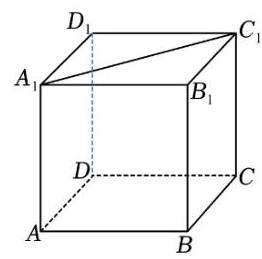
\includegraphics[max width=0.2\textwidth]{images/bo_d5jm9o77aajc7383vmi0_53_1187_451_262_259_0.jpg}
\end{center}
\hspace*{3em} 

【例题】1. (2023 上海春考) 如图所示, \(P\) 是正方体 \({ABCD} - {A}_{1}{B}_{1}{C}_{1}{D}_{1}\) 边 \({A}_{1}{C}_{1}\) 上的动点,下列哪条边与 \({BP}\) 边始终异面 ( )

A. \(D{D}_{1}\) B. \({AC}\)

C. \(A{D}_{1}\) D. \({B}_{1}C\)

【答案】 \(B\)

【解析】当 \(P\) 为 \({A}_{1}{C}_{1}\) 中点时, \(D{D}_{1}\) 和 \({BP}\) 相交;

当 \(P\) 与 \({C}_{1}\) 重合时, \(A{D}_{1}\) 和 \({BP}\) 平行;

当 \(P\) 与 \({C}_{1}\) 重合时, \({B}_{1}C\) 和 \({BP}\) 相交;

只有 \({AC}\) 与 \({BP}\) 边始终异面,故选 \(B\) .

\begin{center}
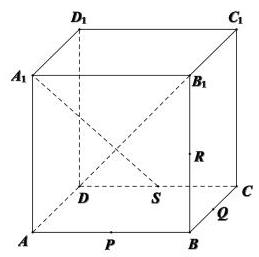
\includegraphics[max width=0.2\textwidth]{images/bo_d5jm9o77aajc7383vmi0_53_1187_887_259_257_0.jpg}
\end{center}
\hspace*{3em} 

【例题】2. (2022 上海秋考) 如图正方体 \({ABCD} - {A}_{1}{B}_{1}{C}_{1}{D}_{1}\) 中, \(P\text{ 、 }Q\text{ 、 }R\text{ 、 }S\) 分别为棱 \({AB}\text{ 、 }{BC}\text{ 、 }{B{B}_{1}}\text{ 、 }{CD}\) 的中点,联结 \({A}_{1}S\text{ 、 }{B}_{1}D\) ,空间任意两点 \(M\text{ 、 }N\) ,若线段 \({MN}\) 上不存在点在线段 \({A}_{1}S\text{ 、 }{B}_{1}D\) 上,则称 \(M\text{ 、 }N\) 两点可视,下列选项中与点 \({D}_{1}\) 可视的为 ( )

A. 点 \(P\) B. 点 \(B\)

C. 点 \(R\) D. 点 \(Q\)

【答案】 \(D\)

【解析】 \(M\text{ 、 }N\) 两点“可视”的定义就是直线 \({MN}\) 不与 \({A}_{1}S\) 相交,也不与 \({B}_{1}D\) 相交, 易得 \({D}_{1}P\) 与 \({A}_{1}S\) 共面，相交； \({D}_{1}R\) 、 \({D}_{1}B\) 均与 \({B}_{1}D\) 共面，相交； \({D}_{1}Q\) 与 \({A}_{1}S\) 异面，也与 \({B}_{1}D\) 异面，故选 \(D\) .

\begin{center}
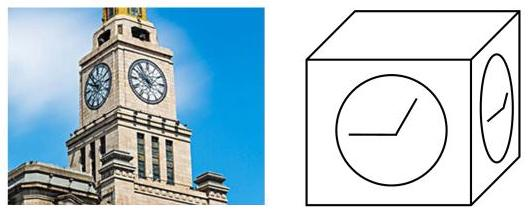
\includegraphics[max width=0.4\textwidth]{images/bo_d5jm9o77aajc7383vmi0_53_931_1377_528_214_0.jpg}
\end{center}
\hspace*{3em} 

【例题】3. (2022 上海春考) 如图所示, 设上海海关楼的钟楼为正方体,且钟楼的四个侧面均有时钟悬挂. 在 0 点到 12 点中时针与分针的转动中 (包括 0 点, 但不包括 12 点), 相邻两面的时针出现垂直的情况的次数为 ( )

A. 0 B. 2

C. 4 D. 12

【答案】 \(B\)

【解析】法一:首先，3 点和 9 点，相邻两面的时针显然垂直，

除 3 点和 9 点外, 若存在其他时刻垂直, 以正方体的前面和右边为例,

不妨设两条时针所在直线为 \(m\) 和 \(n\) ,则 \(m \bot  n\) ,显然后边平面下边直线垂直于 \(m\) , 故 \(m\) 垂直于右边平面,矛盾,故相邻两面的时针出现垂直的情况的次数为 2, 故选 \(B\) .

法二:建立空间直角坐标系，把两个平面放在 \({xOz}\) 平面和 \({yOz}\) 平面，

设时刻为 \(t\) ，由于每小时时针旋转 \(\frac{\pi }{6}\) ，故两个平面内时针所对的坐标分别为

\(\left( {-\cos \left( {-\frac{\pi }{6}t}\right) ,0,0,\sin \left( {-\frac{\pi }{6}t}\right) }\right) ,\left( {0, - \cos \left( {-\frac{\pi }{6}t}\right) ,\sin \left( {-\frac{\pi }{6}t}\right) }\right) ,\)

若相邻两面的时针出现垂直，则数量积为 0，得 \(\sin \left( {-\frac{\pi }{6}t}\right)  = 0\) ,

故 \(t = 0\) 或 \(t = 6\) (注,这里的 \(t\) 是与三角比定义相同的,换算成时间为 3 点和 9 点),

故选 B.

【例题】4. (2021 上海秋考) 已知圆柱的底面圆半径为 1,高为 \(2,{AB}\) 为上底面圆的一条直径， \(C\) 是下底面圆周上的一个动点，则 \(\bigtriangleup  {ABC}\) 的面积的取值范围为\_\_\_\_\_.

【答案】 \(\left\lbrack  {2,\sqrt{5}}\right\rbrack\)

【解析】如图 1,上底面圆心记为 \(O\) ,下底面圆心记为 \({O}^{\prime }\) ,

\begin{center}
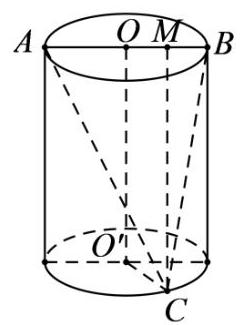
\includegraphics[max width=0.2\textwidth]{images/bo_d5jm9o77aajc7383vmi0_54_308_675_242_325_0.jpg}
\end{center}
\hspace*{3em} 

1

\begin{center}
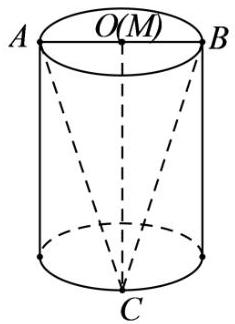
\includegraphics[max width=0.2\textwidth]{images/bo_d5jm9o77aajc7383vmi0_54_581_674_235_324_0.jpg}
\end{center}
\hspace*{3em} 

2

\begin{center}
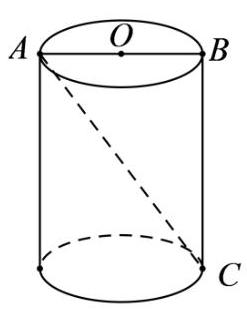
\includegraphics[max width=0.2\textwidth]{images/bo_d5jm9o77aajc7383vmi0_54_849_683_247_310_0.jpg}
\end{center}
\hspace*{3em} 

3

连接 \({OC}\) ,过点 \(C\) 作 \({CM} \bot  {AB}\) ,垂足为点 \(M\) ,则 \({S}_{\Delta ABC} = \frac{1}{2} \times  {AB} \times  {CM}\) ,

\({AB}\) 为定值 2,所以 \({S}_{\Delta ABC}\) 的大小随着 \({CM}\) 的长短变化而变化,

如图 2 所示,当点 \(M\) 与点 \(O\) 重合时, \({CM} = {OC} = \sqrt{{1}^{2} + {2}^{2}} = \sqrt{5}\) ,

此时 \({S}_{\bigtriangleup {ABC}}\) 取得最大值为 \(\frac{1}{2} \times  2 \times  \sqrt{5} = \sqrt{5}\) ;

如图 3 所示,当点 \(M\) 与点 \(B\) 重合, \({CM}\) 取最小值 2,

此时 \({S}_{\bigtriangleup {ABC}}\) 取得最小值为 \(\frac{1}{2} \times  2 \times  2 = 2\) .

综上所述， \({S}_{\Delta ABC}\) 的取值范围为 \(\left\lbrack  {2,\sqrt{5}}\right\rbrack\) .

\begin{center}
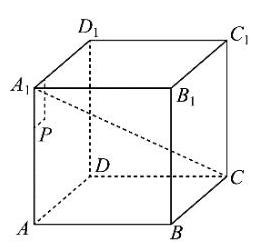
\includegraphics[max width=0.2\textwidth]{images/bo_d5jm9o77aajc7383vmi0_54_1199_1470_253_247_0.jpg}
\end{center}
\hspace*{3em} 

【例题】5. (2020 上海秋考) 在棱长为 10 的正方体 \({ABCD} - {A}_{1}{B}_{1}{C}_{1}{D}_{1}\) 中, \(P\) 为左侧面 \({AD}{D}_{1}{A}_{1}\) 上一点,已知点 \(P\) 到 \({A}_{1}{D}_{1}\) 的距离为 \(3,P\) 到 \(A{A}_{1}\) 的距离为 2, 则过点 \(P\) 且与 \({A}_{1}C\) 平行的直线交正方体于 \(P\text{ 、 }Q\) 两点,则 \(Q\) 点所在的平面是 ( )

A. \(A{A}_{1}{B}_{1}B\) B. \(B{B}_{1}{C}_{1}C\)

C. \(C{C}_{1}{D}_{1}D\) D. \({ABCD}\)

【答案】 \(D\)

【解析】由点 \(P\) 到 \({A}_{1}{D}_{1}\) 的距离为 \(3,P\) 到 \(A{A}_{1}\) 的距离为 2,

\begin{center}
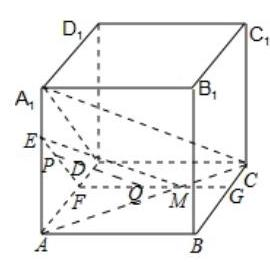
\includegraphics[max width=0.2\textwidth]{images/bo_d5jm9o77aajc7383vmi0_54_1176_1845_270_262_0.jpg}
\end{center}
\hspace*{3em} 

得 \(P\) 在 \(\bigtriangleup A{A}_{1}D\) 内,过 \(P\) 作 \({EF}//{A}_{1}D\) ,且 \({EF} \cap  A{A}_{1}\) 于 \(E,{EF} \cap  {AD}\) 于 \(F\) , 在平面 \({ABCD}\) 中,过 \(F\) 作 \({FG}//{CD}\) ,交 \({BC}\) 于 \(G\) ,则平面 \({EFG}//\) 平面 \({A}_{1}{DC}\) .

连接 \({AC}\) 交 \({FG}\) 于 \(M\) ,连接 \({EM}\) ,

因为平面 \({EFG}//\) 平面 \({A}_{1}{DC}\) ,平面 \({A}_{1}{AC} \cap\) 平面 \({A}_{1}{DC} = {A}_{1}C\) ,

平面 \({A}_{1}{AC} \cap\) 平面 \({EFM} = {EM}\) ,所以 \({EM}//{A}_{1}C\) .

在 \({\Delta EFM}\) 中,过 \(P\) 作 \({PQ}//{EM}\) ,且 \({PQ} \cap  {FM}\) 于 \(Q\) ,则 \({PQ}//{A}_{1}C\) .

因为线段 \({FM}\) 在四边形 \({ABCD}\) 内, \(Q\) 在线段 \({FM}\) 上,所以 \(Q\) 在四边形 \({ABCD}\) 内.

则 \(Q\) 点所在的平面是平面 \({ABCD}\) . 故选 \(D\) .

【例题】6. (2019 上海春考) 已知平面 \(\alpha \text{ 、 }\beta \text{ 、 }\gamma\) 两两垂直,直线 \(a\text{ 、 }b\text{ 、 }c\) 满足: \(a \subseteq  \alpha ,b \subseteq  \beta ,c \subseteq  \gamma\) ,则直线 \(a\text{ 、 }b\text{ 、 }c\) 不可能满足以下哪种关系 ( )

A. 两两垂直 B. 两两平行 C. 两两相交 D. 两两异面

【答案】 \(B\)

\begin{center}
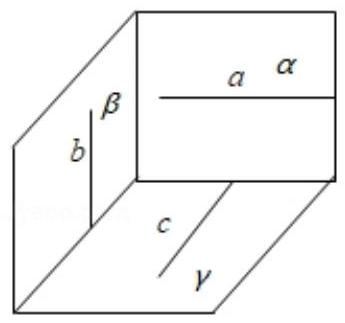
\includegraphics[max width=0.2\textwidth]{images/bo_d5jm9o77aajc7383vmi0_55_288_627_345_323_0.jpg}
\end{center}
\hspace*{3em} 

图 1

\begin{center}
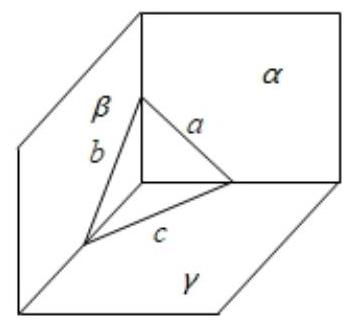
\includegraphics[max width=0.2\textwidth]{images/bo_d5jm9o77aajc7383vmi0_55_703_630_349_323_0.jpg}
\end{center}
\hspace*{3em} 

图2

\begin{center}
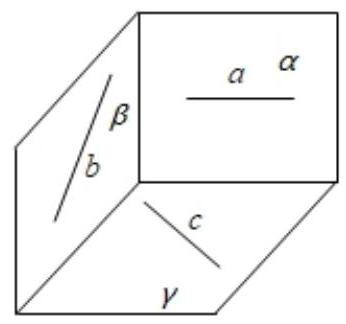
\includegraphics[max width=0.2\textwidth]{images/bo_d5jm9o77aajc7383vmi0_55_1117_624_346_324_0.jpg}
\end{center}
\hspace*{3em} 

图3

【解析】如图 1,得 \(a\text{ 、 }b\text{ 、 }c\) 可能两两垂直; 如图 2,得 \(a\text{ 、 }b\text{ 、 }c\) 可能两两相交; 如图 3,得 \(a\text{ 、 }b\text{ 、 }c\) 可能两两异面; 故选 \(B\) .

【例题】7. (2017 上海春考) 过正方体中心的平面截正方体所得的截面中，不可能的图形是\_\_\_\_\_ (   )

A. 三角形 B. 长方形

C. 对角线不相等的菱形 D. 六边形

【答案】 \(A\)

【解析】过正方体中心的平面截正方体所得的截面, 至少与正方体的四个面相交, 所以不可能是三角形,故选 \(A\) .

\begin{center}
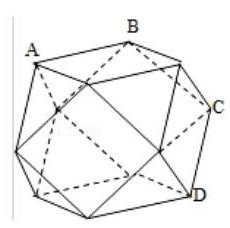
\includegraphics[max width=0.2\textwidth]{images/bo_d5jm9o77aajc7383vmi0_55_1227_1439_230_228_0.jpg}
\end{center}
\hspace*{3em} 

【例题】8. (2011 上海春考) 有一种多面体的饰品,其表面有 6 个正方形和 8 个正三角形组成 (如图)，则 \({AB}\) 与 \({CD}\) 所成的角的大小是\_\_\_\_\_.

【答案】 \(\frac{\pi }{3}\)

【解析】平移后易得所成夹角为 \(\frac{\pi }{3}\) .

\begin{center}
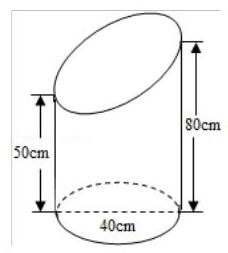
\includegraphics[max width=0.2\textwidth]{images/bo_d5jm9o77aajc7383vmi0_55_1228_1683_228_253_0.jpg}
\end{center}
\hspace*{3em} 

【例题】9. (2010 上海春考) 在如图所示的斜截圆柱中,已知圆柱底面的直径为 40cm，母线长最短 50cm，最长 80cm，则斜截圆柱的侧面面积 \(S =\) \_\_\_\_\_ \({\mathrm{{cm}}}^{2}\) .

【答案】 \({2600\pi }\)

【解析】将相同的两个几何体,对接为圆柱,则圆柱的侧面展开, 侧面展开图的面积 \(S = \left( {{50} + {80}}\right)  \times  {20\pi } \times  2 \times  \frac{1}{2} = {2600\pi c}{m}^{2}\) .

\begin{center}
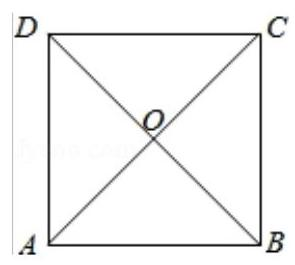
\includegraphics[max width=0.2\textwidth]{images/bo_d5jm9o77aajc7383vmi0_56_1165_236_295_265_0.jpg}
\end{center}
\hspace*{3em} 

【例题】10. (2010 上海秋考) 如图所示,在边长为4的正方形纸片 \({ABCD}\) 中, \({AC}\) 与 \({BD}\) 相交于 \(O\) ,剪去 \(\bigtriangleup {AOB}\) ,将剩余部分沿 \({OC}\text{ 、 }{OD}\) 折叠,使 \({OA}\) 、 \({OB}\) 重合,则以 \(A\left( B\right) \text{ 、 }C\text{ 、 }D\text{ 、 }O\) 为顶点的四面体的体积为\_\_\_\_\_.

【答案】 \(\frac{8\sqrt{2}}{3}\)

【解析】翻折后的几何体为底面边长为 4,侧棱长为 \(2\sqrt{2}\) 的正三棱锥, 高为 \(\frac{2\sqrt{6}}{3}\) 所以该四面体的体积为 \(\frac{1}{3} \times  \frac{1}{2} \times  {16} \times  \frac{\sqrt{3}}{2} \times  \frac{2\sqrt{6}}{3} = \; \frac{8\sqrt{2}}{3}\) .

\section*{2. 模拟练习}

【练习】1. 如图,已知点 \(A \in\) 平面 \(\alpha\) ,点 \(O \in  \alpha\) ,直线 \(a \subset  \alpha\) ,点 \(P \notin  \alpha\) 且 \({PO} \bot  \alpha\) , 则“直线 \(a \bot\) 直线 \({OA}\) ” 是 “直线 \(a \bot\) 直线 \({PA}\) ” 的 ( )

\begin{center}
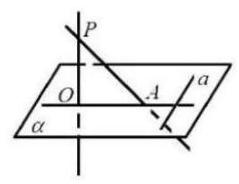
\includegraphics[max width=0.2\textwidth]{images/bo_d5jm9o77aajc7383vmi0_56_326_770_239_184_0.jpg}
\end{center}
\hspace*{3em} 

A. 充分不必要条件 B. 必要不充分条件

C. 充要条件 D. 既不充分也不必要条件

【答案】 \(C\)

【解析】因为 \({PO} \bot  a\) ,所以 \({PO} \bot  a\) ,且 \({PO} \cap  {OA} = O\)

则 \({OA} \bot  a \Leftrightarrow  a \bot\) 平面 \({POA} \Leftrightarrow  a \bot  {PA}\) ,

所以“直线 \(a \bot\) 直线 \({OA}\) ” 是 “直线 \(a \bot\) 直线 \({PA}\) 的充要条件”,故选: \(C\)

【练习】2. 如图,在正方体 \({ABCD} - {A}_{1}{B}_{1}{C}_{1}{D}_{1}\) 中,点 \(M\text{ 、 }N\) 分别在棱 \(A{A}_{1}\text{ 、 }C{C}_{1}\) 上, 则“直线 \({MN} \bot\) 直线 \({C}_{1}B\) ” 是“直线 \({MN} \bot\) 平面 \({C}_{1}{BD}\) ” 的 ( )

\begin{center}
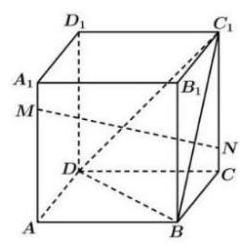
\includegraphics[max width=0.2\textwidth]{images/bo_d5jm9o77aajc7383vmi0_56_322_1353_244_245_0.jpg}
\end{center}
\hspace*{3em} 

A. 充分非必要条件 B. 必要非充分条件

C. 充要条件 D. 既不充分又不必要条件

【答案】 \(C\)

【解析】首先必要性是满足的, 由线面垂直的性质定理 (或定义) 易得; 下面说明充分性, 连接 \({AC},{A}_{1}{C}_{1},A{A}_{1} \bot\) 平面 \({ABCD},{BD} \subset\) 平面 \({ABCD}\) ,则 \(A{A}_{1} \bot  {BD}\) ,

\begin{center}
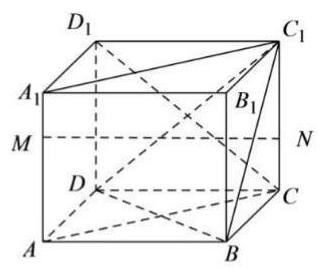
\includegraphics[max width=0.2\textwidth]{images/bo_d5jm9o77aajc7383vmi0_57_325_237_320_269_0.jpg}
\end{center}
\hspace*{3em} 

正方形中 \({BD} \bot  {AC},{AC} \cap  A{A}_{1} = A,{AC},A{A}_{1} \subset\) 平面 \({AC}{C}_{1}{A}_{1}\) ,

则 \({BD} \bot\) 平面 \({AC}{C}_{1}{A}_{1}\) ,

又 \({MN} \subset\) 平面 \({AC}{C}_{1}{A}_{1}\) ,所以 \({BD} \bot  {MN}\) ,

若 \({MN}\bot {B{C}_{1}},{B{C}_{1}} \cap  {BD} = B,B{C}_{1},{BD} \subset\) 平面 \({BD}{C}_{1}\) ，所以 \({MN}\bot\) 平面 \({BD}{C}_{1}\) ，充分性得证. 因此应为充要条件. 故选: \(C\) .

【练习】3. 类比平面内“垂直于同条一直线的两条直线互相平行”的性质，可推出空间中有下列结论:

 \circled{1} 垂直于同一条直线的两条直线互相平行；

 \circled{2} 垂直于同一条直线的两个平面互相平行；

 \circled{3} 垂直于同一个平面的两条直线互相平行;

 \circled{4} 垂直于同一个平面的两个平面互相平行.

其中正确的是 ( )

A.  \circled{1}  \circled{2}  B.  \circled{2}  \circled{3}  C.  \circled{3}  \circled{4}  D.  \circled{1}  \circled{4} 

【答案】 \(B\)

【解析】垂直于同一条直线的两条直线平行、相交、或异面,  \circled{1} 错误;

垂直于同一个平面的两条直线互相平行, 由直线与平面平行的性质知 \circled{2} 正确;

垂直于同一条直线的两个平面互相平行, 由平面平行的判定定理知

垂直于同一个平面的两个平面平行或相交,  \circled{4} 错误;

故选: \(B\)

【练习】4. 已知直线 \(a,b,l\) 和平面 \(\alpha ,\beta ,a \subset  \alpha ,b \subset  \beta ,\alpha  \cap  \beta  = l\) ,且 \(\alpha  \bot  \beta\) ;

 \circled{1} 若 \(a,b\) 异面，则 \(a,b\) 至少有一个与 \(l\) 相交；

 \circled{2} 若 \(a,b\) 垂直，则 \(a,b\) 至少有一个与 \(l\) 垂直；对于以上命题中，所有正确的序号是\_\_\_\_\_

【答案】 \circled{1}  \circled{2} 

【解析】若 \(a,b\) 与 \(l\) 都不相交, \(a \subset  \alpha ,l \subset  \alpha\) ,则 \(a//l\) ,

\begin{center}
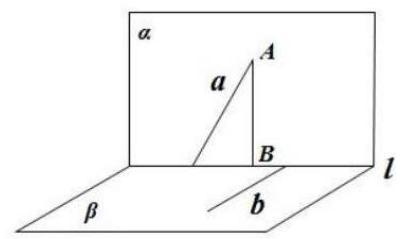
\includegraphics[max width=0.3\textwidth]{images/bo_d5jm9o77aajc7383vmi0_57_324_1591_403_239_0.jpg}
\end{center}
\hspace*{3em} 

同理 \(b//l\) ,故 \(a//b\) ,与 \(a,b\) 异面矛盾, \circled{1} 正确;

若 \(a\) 不垂直 \(l,a\) 上取一点 \(A\) ,作 \({AB} \bot  l\) 交 \(l\) 于 \(B,{AB} \bot  l,\alpha  \bot  \beta\) ,

故 \({AB} \bot  \beta ,b \subset  \beta\) ,故 \({AB} \bot  b,b \bot  a,a \cap  {AB} = A\) ,

故 \(b \bot  \alpha ,\alpha  \bot  \beta ,b \subset  \beta\) ,故 \(b \bot  l\) , \circled{2}  正确.

故答案为: \circled{1}  \circled{2} .

【练习】5. 下列命题中,正确的是 ( )

A. 三点确定一个平面

B. 垂直于同一直线的两条直线平行

C. 若直线 \(l\) 与平面 \(\alpha\) 上的无数条直线都垂直，则 \(l\bot \alpha\)

D. 若 \(a\text{ 、 }b\text{ 、 }c\) 是三条直线， \(a//b\) 且与 \(c\) 都相交，则直线 \(a\text{ 、 }b\text{ 、 }c\) 在同一平面上

【答案】 \(D\)

【解析】 \(A\) . 不共线的三点确定一个平面; \(B\) . 由墙角模型得显然错误;

C. 必须和所有直线垂直，不是无数条直线垂直，事实上，平面的斜线也和平面内无数条直线垂直 (由三垂直定理易证)；

\(D\) . 由平面公理,两条平行直线唯一确定一个平面,

两条相交直线唯一确定一个平面,正确;

故选 \(D\) .

【练习】6. (2024 届控江)在正方体 \({ABCD} - {A}_{1}{B}_{1}{C}_{1}{D}_{1}\) 中， \(E\) 、 \(F\) 分别为棱 \(A{A}_{1}\) 、 \(C{C}_{1}\) 的中点，则在空间中与三条直线 \({A}_{1}{D}_{1}\text{ 、 }{EF}\text{ 、 }{CD}\) 都相交的直线 ( )

A. 不存在 B. 有且只有两条 C. 有且只有三条 D. 有无数条

\begin{center}
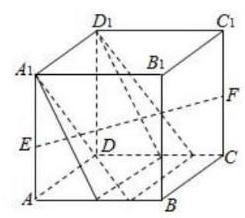
\includegraphics[max width=0.2\textwidth]{images/bo_d5jm9o77aajc7383vmi0_58_1218_958_245_218_0.jpg}
\end{center}
\hspace*{3em} 

【答案】 \(D\)

【解析】在 \({EF}\) 上任意取一点 \(M\) ,直线 \({A}_{1}{D}_{1}\) 与 \(M\) 确定一个平面,

这个平面与 \({CD}\) 有且仅有 1 个交点 \(N\) ,

当 \(M\) 取不同的位置就确定不同的平面,从而与 \({CD}\) 有不同的交点 \(N\) , 而直线 \({MN}\) 与这 3 条异面直线都有交点. 故选 \(D\) .

【练习】7. 如图. 空间四边形 \({OABC}\) 中, \(\overrightarrow{OA} = \overrightarrow{a},\overrightarrow{OB} = \overrightarrow{b},\overrightarrow{OC} = \overrightarrow{c}\) ,点 \(M\) 在 \({OA}\) 上, 且满足 \(\overrightarrow{OM} = 2\overrightarrow{MA}\) ,点 \(N\) 为 \({BC}\) 的中点,则 \(\overrightarrow{MN} =\) ( )

\begin{center}
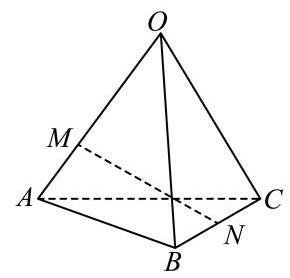
\includegraphics[max width=0.2\textwidth]{images/bo_d5jm9o77aajc7383vmi0_58_288_1297_290_278_0.jpg}
\end{center}
\hspace*{3em} 

A. \(\frac{1}{2}\overrightarrow{a} - \frac{2}{3}\overrightarrow{b} + \frac{1}{2}\overrightarrow{c}\) B. \(\frac{2}{3}\overrightarrow{a} + \frac{2}{3}\overrightarrow{b} - \frac{1}{2}\overrightarrow{c}\)

C. \(\frac{1}{2}\overrightarrow{a} + \frac{1}{2}\overrightarrow{b} - \frac{1}{2}\overrightarrow{c}\) D. \(- \frac{2}{3}\overrightarrow{a} + \frac{1}{2}\overrightarrow{b} + \frac{1}{2}\overrightarrow{c}\)

【答案】 \(D\)

【解析】 \(\overrightarrow{MN} = \overrightarrow{ON} - \overrightarrow{OM} = \frac{1}{2}\left( {\overrightarrow{OB} + \overrightarrow{OC}}\right)  - \frac{2}{3}\overrightarrow{OA} =  - \frac{2}{3}\overrightarrow{a} + \frac{1}{2}\overrightarrow{b} + \frac{1}{2}\overrightarrow{c}\) . 故选: \(D\) .

【练习】8. 用斜二测画法画出的某平面图形的直观图如图所示,边 \({A}^{\prime }{B}^{\prime }\) 与 \({C}^{\prime }{D}^{\prime }\) 平行于 \({x}^{\prime }\) 轴. 已知四边形 \({A}^{\prime }{B}^{\prime }{C}^{\prime }{D}^{\prime }\) 的面积为 \(1{\mathrm{\;{cm}}}^{2}\) ，则原平面图形的面积为\_\_\_\_\_ \({\mathrm{{cm}}}^{2}\)

2025 版上海高考真题及模拟训练合集(下册)

\begin{center}
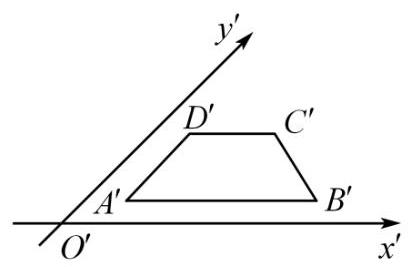
\includegraphics[max width=0.3\textwidth]{images/bo_d5jm9o77aajc7383vmi0_59_288_229_409_267_0.jpg}
\end{center}
\hspace*{3em} 

【答案】 \(2\sqrt{2}\)

【解析】根据题意得 \(\angle {B}^{\prime }{A}^{\prime }{D}^{\prime } = {45}^{ \circ  }\) ,原四边形为一个直角梯形,

\begin{center}
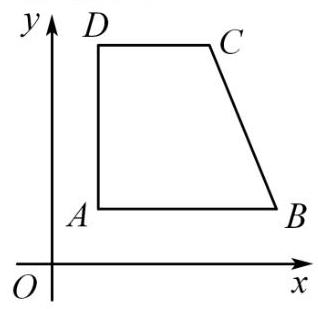
\includegraphics[max width=0.2\textwidth]{images/bo_d5jm9o77aajc7383vmi0_59_290_587_318_309_0.jpg}
\end{center}
\hspace*{3em} 

且 \({CD} = {C}^{\prime }{D}^{\prime },{AB} = {A}^{\prime }{B}^{\prime },{AD} = 2{A}^{\prime }{D}^{\prime }\) ,

\({S}_{\text{ 梯形 }{A}^{\prime }{B}^{\prime }{C}^{\prime }{D}^{\prime }} = \frac{1}{2}\left( {{A}^{\prime }{B}^{\prime } + {C}^{\prime }{D}^{\prime }}\right)  \cdot  {A}^{\prime }{D}^{\prime }\sin {45}^{ \circ  } = \frac{\sqrt{2}}{4}\left( {{A}^{\prime }{B}^{\prime } + {C}^{\prime }{D}^{\prime }}\right)  \cdot  {A}^{\prime }{D}^{\prime } = 1\left( {\mathrm{\;{cm}}}^{2}\right)\) ,

则 \(\left( {{A}^{\prime }{B}^{\prime } + {C}^{\prime }{D}^{\prime }}\right)  \cdot  {A}^{\prime }{D}^{\prime } = 2\sqrt{2}\) ,

所以， \({S}_{\text{ 梯形 }{ABCD}} = \frac{1}{2}\left( {{AB} + {CD}}\right)  \cdot  {AD} = \frac{1}{2}\left( {{A}^{\prime }{B}^{\prime } + {C}^{\prime }{D}^{\prime }}\right)  \cdot  {2{A}^{\prime }{D}^{\prime }} = \left( {{A}^{\prime }{B}^{\prime } + {C}^{\prime }{D}^{\prime }}\right)  \cdot  {{A}^{\prime }{D}^{\prime }} = \; 2\sqrt{2}\left( {\mathrm{\;{cm}}}^{2}\right) .\)

故答案为: \(2\sqrt{2}\) .

【练习】9. 如图所示，在正三棱柱 \({ABC} - {A}_{1}{B}_{1}{C}_{1}\) 中， \({AB} = 2,A{A}_{1} = 2\) ，由顶点 \(B\) 沿棱柱侧面 (经过棱 \(A{A}_{1}\) ) 到达顶点 \({C}_{1}\) ，与 \(A{A}_{1}\) 的交点记为 \(M\) ，则从点 \(B\) 经点 \(M\) 到 \({C}_{1}\) 的最短路线长为\_\_\_\_\_

\begin{center}
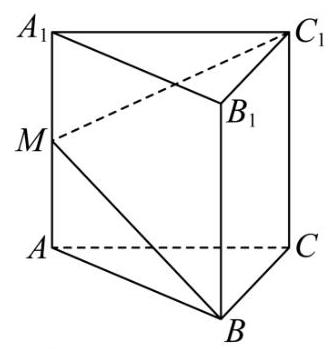
\includegraphics[max width=0.2\textwidth]{images/bo_d5jm9o77aajc7383vmi0_59_291_1365_330_349_0.jpg}
\end{center}
\hspace*{3em} 

【答案】 \(2\sqrt{5}\)

【解析】如图,沿侧棱 \(B{B}_{1}\) 将正三棱柱的侧面展开

\begin{center}
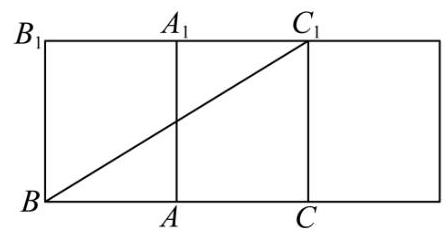
\includegraphics[max width=0.3\textwidth]{images/bo_d5jm9o77aajc7383vmi0_59_291_1810_448_236_0.jpg}
\end{center}
\hspace*{3em} 

由侧面展开图可知,当 \(B,M,{C}_{1}\) 三点共线时,从点 \(B\) 经点 \(M\) 到 \({C}_{1}\) 的路线最短.

所以最短路线长为 \(B{C}_{1} = \sqrt{{4}^{2} + {2}^{2}} = 2\sqrt{5}\) .

【练习】10. 如图,已知正四棱柱 \({ABCD} - {{A}_{1}{B}_{1}{C}_{1}{D}_{1}}\) 的底面边长为 2,高为 3, 则异面直线 \(A{A}_{1}\) 与 \(B{D}_{1}\) 所成角的大小是\_\_\_\_\_

\begin{center}
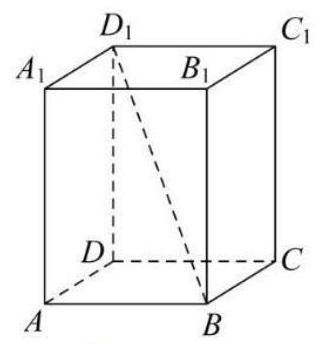
\includegraphics[max width=0.2\textwidth]{images/bo_d5jm9o77aajc7383vmi0_60_325_394_320_344_0.jpg}
\end{center}
\hspace*{3em} 

【答案】 \(\arctan \frac{2\sqrt{2}}{3}\)

【解析】因为 \(A{A}_{1}//D{D}_{1}\) ,所以 \(\angle D{D}_{1}B\) 异面直线 \(A{A}_{1}\) 与 \(B{D}_{1}\) 所成的角,

在正四棱柱 \({ABCD} - {A}_{1}{B}_{1}{C}_{1}{D}_{1}\) 的底面边长为2,高为3,

所以 \(\tan \angle D{D}_{1}B = \frac{BD}{D{D}_{1}} = \frac{2\sqrt{2}}{3}\) ，因为 \(\angle D{D}_{1}B \in  \left( {0,\frac{\pi }{2}}\right)\) ，所以 \(\angle D{D}_{1}B = \arctan \frac{2\sqrt{2}}{3}\) .

2025 版上海高考真题及模拟训练合集(下册)

\section*{板块二: 中档客观题}

\section*{1. 真题回顾}

【例题】1. (2025 上海春考) 已知 \(P\) 是一个圆锥的顶点， \({PA}\) 是母线， \({PA} = 2\) ，该圆锥的底面半径是 1 . \(B,C\) 分别在圆锥的底面上，则异面直线 \({PA}\) 与 \({BC}\) 所成角的最小值为\_\_\_\_\_.

【答案】 \(\frac{\pi }{3}\)

【解析】解法一(空间向量): 以底面圆心 \(O\) 为原点建系,则 \(\overrightarrow{BC}\) 可为底面任意方向,

易得 \(A\left( {-1,0,0}\right) ,P\left( {0,0,\sqrt{3}}\right)\) ,设 \(\overrightarrow{BC} = \left( {\cos \theta ,\sin \theta ,0}\right) ,\overrightarrow{AP} = \left( {1,0,\sqrt{3}}\right)\) ,

则 \(\cos \langle \overrightarrow{AP},\overrightarrow{BC}\rangle  = \frac{\overrightarrow{AP} \cdot  \overrightarrow{BC}}{\left| \overrightarrow{AP}\right|  \cdot  \left| \overrightarrow{BC}\right| } = \frac{\cos \theta }{2} \leq  \frac{1}{2},\therefore \langle \overrightarrow{AP},\overrightarrow{BC}\rangle  \geq  \frac{\pi }{3}\) .

解法二: 依题意可得: 异面直线 \({PA}\) 与 \({BC}\) 所成角的最小值即为直线 \({PA}\) 与底面所成角.

由 \({PA} = 2\) ，底面半径为 1，所以直线 \({PA}\) 与底面所成角为 \(\frac{\pi }{3}\) .

【例题】2. (2024 上海秋考) 已知空间直角坐标系 \({Oxyz}\) 中的点集 \(\Omega\) ，对任意 \({P}_{1},{P}_{2},{P}_{3} \in  \Omega\) ，均存在不全为零的实数 \({\lambda }_{1},{\lambda }_{2},{\lambda }_{3}\) 满足 \({\lambda }_{1}\overrightarrow{O{P}_{1}} + {\lambda }_{2}\overrightarrow{O{P}_{2}} + {\lambda }_{3}\overrightarrow{O{P}_{3}} = \overrightarrow{0}\) . 已知 \(\left( {1,0,0}\right)  \in  \Omega\) ,则 \(\left( {0,0,1}\right)  \notin  \Omega\) 的一个充分条件是 ( )

A. \(\left( {0,0,0}\right)  \in  \Omega\) B. \(\left( {-1,0,0}\right)  \in  \Omega\) C. \(\left( {0, - 1,0}\right)  \in  \Omega\) D. \(\left( {0,0, - 1}\right)  \in  \Omega\)

【答案】 \(C\)

【解析】对任意 \({P}_{1},{P}_{2},{P}_{3} \in  \Omega\) ,均存在不全为零的实数 \({\lambda }_{1},{\lambda }_{2},{\lambda }_{3}\) 满足

\({\lambda }_{1}\overrightarrow{O{P}_{1}} + {\lambda }_{2}\overrightarrow{O{P}_{2}} + {\lambda }_{3}\overrightarrow{O{P}_{3}} = \overrightarrow{0}\) 指的是 \(\overrightarrow{O{P}_{1}},\overrightarrow{O{P}_{2}},\overrightarrow{O{P}_{3}}\) 共面,

可以借助空间直角坐标系分析, \(\left( {1,0,0}\right)\) 在 \(x\) 轴上, \(\left( {0,0,1}\right)\) 在 \(z\) 轴上,

\(\left( {0,0,0}\right)\) 为原点,错误; \(\left( {-1,0,0}\right)\) 在 \(x\) 轴上,错误; \(\left( {0, - 1,0}\right)\) 在 \(y\) 轴上,正确;

\(\left( {0,0, - 1}\right)\) 在 \(z\) 轴上,错误; 故选 \(C\) .

\begin{center}
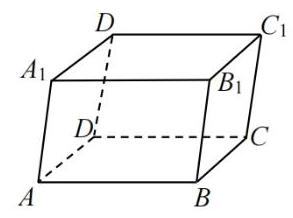
\includegraphics[max width=0.2\textwidth]{images/bo_d5jm9o77aajc7383vmi0_61_1156_1333_293_218_0.jpg}
\end{center}
\hspace*{3em} 

【例题】3. (2024 上海春考) 如图,已知四棱柱 \({ABCD} - {A}_{1}{B}_{1}{C}_{1}{D}_{1}\) 的底面为平行四边形, \(\left| \overrightarrow{A{A}_{1}}\right|  = 3,\left| \overrightarrow{BD}\right|  = 4\) ,且 \(\overrightarrow{A{B}_{1}} \cdot  \overrightarrow{{B}_{1}{C}_{1}} - \overrightarrow{B{C}_{1}} \cdot  \overrightarrow{DC} = 5\) ,则异面直线 \(A{A}_{1}\) 与 \({BD}\) 所成角的大小为\_\_\_\_\_.

【答案】 \(\arccos \frac{5}{12}\)

【解析】 \(\overrightarrow{A{B}_{1}} \cdot  \overrightarrow{{B}_{1}{C}_{1}} - \overrightarrow{B{C}_{1}} \cdot  \overrightarrow{DC}\)

\(= \left( {\overrightarrow{A{A}_{1}} + \overrightarrow{AB}}\right)  \cdot  \overrightarrow{AD} - \left( {\overrightarrow{AD} + \overrightarrow{A{A}_{1}}}\right)  \cdot  \overrightarrow{AB}\)

\(= \overrightarrow{A{A}_{1}} \cdot  \overrightarrow{AD} - \overrightarrow{A{A}_{1}} \cdot  \overrightarrow{AB} = \overrightarrow{A{A}_{1}} \cdot  \overrightarrow{BD} = \left| \overrightarrow{A{A}_{1}}\right|  \cdot  \left| \overrightarrow{BD}\right|  \cdot  \cos \theta  = {12}\cos \theta\) ,

所以 \(\cos \theta  = \frac{5}{12}\) ,所以直线 \(A{A}_{1}\) 与 \({BD}\) 所成角 \(\cos \theta  = \frac{5}{12} \Rightarrow  \theta  = \arccos \frac{5}{12}\) .

\begin{center}
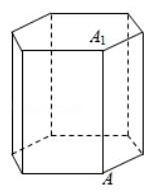
\includegraphics[max width=0.2\textwidth]{images/bo_d5jm9o77aajc7383vmi0_62_1304_234_150_192_0.jpg}
\end{center}
\hspace*{3em} 

【例题】4. (2018 上海秋考) 《九章算术》中, 称底面为矩形而有一侧棱垂直于底面的四棱锥为阳马，设 \(A{A}_{1}\) 是正六棱柱的一条侧棱,如图，若阳马以该正六棱柱的顶点为顶点、以 \(A{A}_{1}\) 为底面矩形的一边,则这样的阳马的个数是 ( )

A. 4 B. 8 C. 12 D. 16

【答案】 \(D\)

\begin{center}
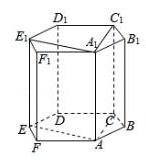
\includegraphics[max width=0.2\textwidth]{images/bo_d5jm9o77aajc7383vmi0_62_1310_480_146_160_0.jpg}
\end{center}
\hspace*{3em} 

【解析】由正六边形的性质,得 \({D}_{1} - {A}_{1}{AB}{B}_{1},{D}_{1} - {A}_{1}{AF}{F}_{1}\) 满足题意,

而 \({C}_{1}\text{ 、 }{E}_{1}\text{ 、 }C\text{ 、 }D\text{ 、 }E\) ,和 \({D}_{1}\) 一样,有 \(2 \times  4 = 8\) ,

当 \({A}_{1}{AC}{C}_{1}\) 为底面矩形,有 4 个满足题意,

当 \({A}_{1}{AE}{E}_{1}\) 为底面矩形,有 4 个满足题意,

故有 \(8 + 4 + 4 = {16}\) 个,故选 \(D\) .

\begin{center}
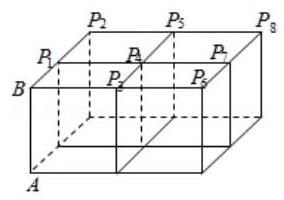
\includegraphics[max width=0.2\textwidth]{images/bo_d5jm9o77aajc7383vmi0_62_1172_747_284_200_0.jpg}
\end{center}
\hspace*{3em} 

【例题】5. (2014 上海秋考) 如图, 四个棱长为 1 的正方体排成一个正四棱柱, \({AB}\) 是一条侧棱, \({P}_{i}\left( {\mathrm{i} = 1,2,\cdots ,8}\right)\) 是上底面上其余的八个点,则 \(\overrightarrow{AB}\) . \({\overrightarrow{AP}}_{i}\left( {\mathrm{i} = 1,2,\cdots ,8}\right)\) 的不同值的个数为 ( )

A. 1 B. 2

C. 3 D. 4

【答案】 \(A\)

【解析】 \(\overrightarrow{A{P}_{i}} = \overrightarrow{AB} + \overrightarrow{B{P}_{i}}\) ,则 \(\overrightarrow{AB} \cdot  \overrightarrow{A{P}_{i}} = \overrightarrow{AB}\left( {\overrightarrow{AB} + \overrightarrow{B{P}_{i}}}\right)  = {\left| \overrightarrow{AB}\right| }^{2} + \overrightarrow{AB} \cdot  \overrightarrow{B{P}_{i}}\) ,

因为 \(\overrightarrow{AB} \bot  \overrightarrow{B{P}_{i}}\) ,所以 \(\overrightarrow{AB} \cdot  \overrightarrow{A{P}_{i}} = {\left| \overrightarrow{AB}\right| }^{2} = 1\) ,

所以 \(\overrightarrow{AB} \cdot  \overrightarrow{A{P}_{i}}\left( {\mathrm{i} = 1,2,\cdots ,8}\right)\) 的不同值的个数为 1,故选 \(A\) .

【例题】6. (2013 上海秋考) 在 \({xOy}\) 平面上,将两个半圆弧 \({\left( x - 1\right) }^{2} \; + {y}^{2} = 1\left( {x \geq  1}\right)\) 和 \({\left( x - 3\right) }^{2} + {y}^{2} = 1\left( {x \geq  3}\right)\) ,两条直线 \(y = 1\) 和 \(y =  - 1\) 围成的封闭图形记为 \(D\) ,如图中阴影部分,记 \(D\) 绕 \(y\) 轴旋转一周而成的几何体为 \(\Omega\) . 过 \(\left( {0,y}\right) \left( {\left| y\right|  \leq  1}\right)\) 作 \(\Omega\) 的水平截面,所得截面积为 \({4\pi }\sqrt{1 - {y}^{2}} + {8\pi }\) . 试利用祖暅原理、一个平放的圆柱和一个长方体，得出 \(\Omega\) 的体积值为\_\_\_\_\_.

\begin{center}
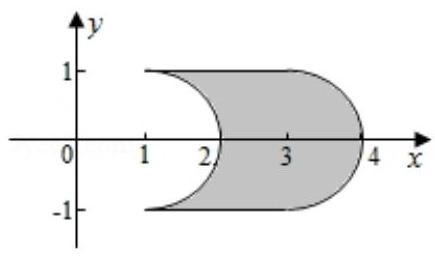
\includegraphics[max width=0.3\textwidth]{images/bo_d5jm9o77aajc7383vmi0_62_1019_1211_435_256_0.jpg}
\end{center}
\hspace*{3em} 

【答案】 \(2{\pi }^{2} + {16\pi }\)

【解析】因为几何体为 \(\Omega\) 的水平截面的截面积为 \({4\pi }\sqrt{1 - {y}^{2}} + {8\pi }\) ,

该截面的截面积由两部分组成，一部分为定值 \({8\pi }\) ，看作是截一个底面积为 \({8\pi }\) ，

高为 2 的长方体得到的，对于 \({4\pi }\sqrt{1 - {y}^{2}}\) ，看作是把一个半径为 1 ，

高为 \({2\pi }\) 的圆柱平放得到的，如图所示，

\begin{center}
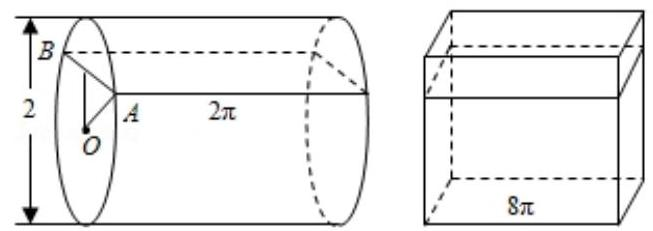
\includegraphics[max width=0.5\textwidth]{images/bo_d5jm9o77aajc7383vmi0_62_290_1734_653_231_0.jpg}
\end{center}
\hspace*{3em} 

这两个几何体与 \(\Omega\) 放在一起，由祖暅原理，每个平行水平面的截面积相等，

故它们的体积相等，即 \(\Omega\) 的体积为 \(\pi  \cdot  {1}^{2} \cdot  {2\pi } + 2 \cdot  {8\pi } = 2{\pi }^{2} + {16\pi }\) . 2025 版上海高考真题及模拟训练合集(下册)

\section*{2. 模拟练习}

\begin{center}
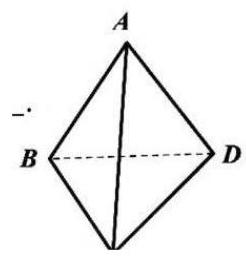
\includegraphics[max width=0.2\textwidth]{images/bo_d5jm9o77aajc7383vmi0_63_1206_313_246_256_0.jpg}
\end{center}
\hspace*{3em} 

【练习】1. (2024 届华二) 已知四面体 \({ABCD}\) 中, \({AB} = 3,{CD} = 2\) ,则 \(\overrightarrow{BC} \cdot  \overrightarrow{AD} - \; \overrightarrow{BD} \cdot  \overrightarrow{AC}\) 的取值范围是\_\_\_\_\_

【答案】 \(\left( {-6,6}\right)\)

【解析】 \(\overrightarrow{BC} \cdot  \overrightarrow{AD} - \overrightarrow{BD} \cdot  \overrightarrow{AC} = \overrightarrow{BC} \cdot  \left( {\overrightarrow{BD} - \overrightarrow{BA}}\right)  - \overrightarrow{BD} \cdot  \left( {\overrightarrow{BC} - \overrightarrow{BA}}\right)\)

\(= \overrightarrow{BD} \cdot  \overrightarrow{BA} - \overrightarrow{BC} \cdot  \overrightarrow{BA} = \overrightarrow{CD} \cdot  \overrightarrow{BA} \in  \left( {-6,6}\right)\) .

\begin{center}
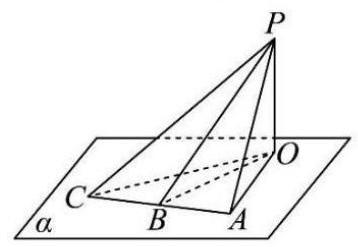
\includegraphics[max width=0.3\textwidth]{images/bo_d5jm9o77aajc7383vmi0_63_1096_567_358_247_0.jpg}
\end{center}
\hspace*{3em} 

【练习】2. 如图,已知 \({PA}\text{ 、 }{PB}\text{ 、 }{PC}\) 与平面 \(\alpha\) 所成角分别为 \({60}^{ \circ  }\text{ 、 }{45}^{ \circ  }\text{ 、 }{30}^{ \circ  }\) , \({PO} \bot\) 平面 \(\alpha ,O\) 为垂足,又有斜足 \(A\text{ 、 }B\text{ 、 }C\) 三点在同一直线上, 且 \({AB} = {BC} = {10}\mathrm{\;{cm}}\) ，则 \({PO}\) 的长等于\_\_\_\_\_.

【答案】 \(5\sqrt{6}\)

【解析】设 \({PO} = x\) ,则 \({PA} = \frac{2}{\sqrt{3}}x,{PB} = \sqrt{2}x,{PC} = {2x}\) ,

又 \({PB}\) 是 \(\bigtriangleup {PAC}\) 底边 \({AC}\) 上的中线,则 \(2\overrightarrow{PB} = \overrightarrow{PC} + \overrightarrow{PA},\overrightarrow{AC} = \overrightarrow{AP} \; + \overrightarrow{PC}\) ,

\({\left( 2\overrightarrow{PB}\right) }^{2} = {\left( \overrightarrow{PC} + \overrightarrow{PA}\right) }^{2} = {\overrightarrow{PC}}^{2} + 2\overrightarrow{PC} \cdot  \overrightarrow{PA} + {\overrightarrow{PA}}^{2},\)

\({\left( \overrightarrow{AC}\right) }^{2} = {\left( \overrightarrow{AP} + \overrightarrow{PC}\right) }^{2} = {\overrightarrow{AP}}^{2} + 2\overrightarrow{AP} \cdot  \overrightarrow{PC} + {\overrightarrow{PC}}^{2} = {\overrightarrow{AP}}^{2} - 2\overrightarrow{PA} \cdot  \overrightarrow{PC} + {\overrightarrow{PC}}^{2}\) ,

所以 \(4\overrightarrow{PB}{}^{2} + \overrightarrow{AC}{}^{2} = 2\overrightarrow{PC}{}^{2} + 2\overrightarrow{PA}{}^{2}\) ,则 \(4\overrightarrow{PB}{}^{2} = 2\overrightarrow{PC}{}^{2} + 2\overrightarrow{PA}{}^{2} - \overrightarrow{AC}{}^{2}\) ,

所以 \(8{x}^{2} = 8{x}^{2} + \frac{8}{3}{x}^{2} - {400}\) ,故 \(x = 5\sqrt{6}\) ,所以 \({PO} = 5\sqrt{6}\) .

【练习】3. (2024 届曹二) 在棱长为 2 的正方体 \({ABCD} - {A}_{1}{B}_{1}{C}_{1}{D}_{1}\) 中,点 \(P\) 在正方体的 12 条棱上 (包括顶点) 运动，则 \(\overrightarrow{AC} \cdot  \overrightarrow{BP}\) 的取值范围是\_\_\_\_\_.

【答案】 \(\left\lbrack  {-4,4}\right\rbrack\)

【解析】以 \(D\) 为坐标原点建立空间直角坐标系,

\begin{center}
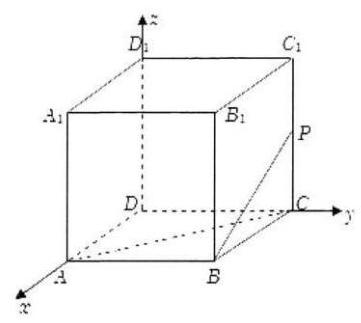
\includegraphics[max width=0.3\textwidth]{images/bo_d5jm9o77aajc7383vmi0_63_1095_1314_361_323_0.jpg}
\end{center}
\hspace*{3em} 

则 \(A\left( {2,0,0}\right) ,C\left( {0,2,0}\right) ,B\left( {2,2,0}\right) ,\overrightarrow{AC} = \left( {-2,2,0}\right)\) ,

\(P\) 在正方体的 12 条棱上运动,设 \(P\left( {x,y,z}\right)\) ,则 \(\overrightarrow{BP} = \; \left( {x - 2,y - 2,z}\right)\) ,

所以 \(\overrightarrow{AC} \cdot  \overrightarrow{BP} = 4 - {2x} + {2y} - 4 = {2y} - {2x}\) ,

因为 \(\left\{  \begin{array}{l} 0 \leq  x \leq  2 \\  0 \leq  y \leq  2 \end{array}\right.\) ,所以 \(- 4 \leq  {2y} - {2x} \leq  4\) ,

当 \(x = 2,y = 0\) 时, \(\overrightarrow{AC} \cdot  \overrightarrow{BP}\) 取最小值 -4,

当 \(x = 0,y = 2\) 时, \(\overrightarrow{AC} \cdot  \overrightarrow{BP}\) 取最大值 4,

所以 \(\overrightarrow{AC} \cdot  \overrightarrow{BP}\) 的取值范围是 \(\left\lbrack  {-4,4}\right\rbrack\) .

【练习】4. (2024 届奉中) 在 \(\bigtriangleup  {ABC}\) 中，各个顶点与对边中点连线，相交于一点，定义为三角形的重心 \(G\) ,此时易得 \(\overrightarrow{AG} = \frac{1}{3}\left( {\overrightarrow{AB} + \overrightarrow{AC}}\right)\) . 类似在三棱锥 \(P - {ABC}\) 中,各个顶点分别与对面三角形的重心的连线，相交于一点，定义为三棱在的重心 \(G\) . 若设 \(\overrightarrow{PA} = \overrightarrow{a}\) ， \(\overrightarrow{PB} = \overrightarrow{b}\) ， \(\overrightarrow{PC} = \overrightarrow{c}\) ，则 \(\overrightarrow{PG} =\) \_\_\_\_\_(用 \(\overrightarrow{a}\text{ 、 }\overrightarrow{b}\text{ 、 }\overrightarrow{c}\) 表示).

【答案】 \(\frac{1}{4}\overrightarrow{a} + \frac{1}{4}\overrightarrow{b} + \frac{1}{4}\overrightarrow{c}\)

【解析】设点 \(D\) 为 \(\bigtriangleup  {ABC}\) 的重心，点 \(E\) 为 \(\bigtriangleup  {PBC}\) 的重心，

\(\overrightarrow{PD} = \overrightarrow{PA} + \overrightarrow{AD} = \overrightarrow{PA} + \frac{1}{3}\left( {\overrightarrow{AB} + \overrightarrow{AC}}\right)  = \overrightarrow{PA} + \frac{1}{3}\left( {\overrightarrow{PB} - \overrightarrow{PA} + \overrightarrow{PC} - \overrightarrow{PA}}\right) ,\)

\(= \frac{1}{3}\overrightarrow{a} + \frac{1}{3}\overrightarrow{b} + \frac{1}{3}\overrightarrow{c},\overrightarrow{AE} = \overrightarrow{AP} + \overrightarrow{PE} =  - \overrightarrow{PA} + \frac{1}{3}\left( {\overrightarrow{PB} + \overrightarrow{PC}}\right)  =  - \overrightarrow{a} + \frac{1}{3}\overrightarrow{b} + \frac{1}{3}\overrightarrow{c}\) ,

设 \(\overrightarrow{PG} = \lambda \overrightarrow{PD} = \frac{\lambda }{3}\overrightarrow{a} + \frac{\lambda }{3}\overrightarrow{b} + \frac{\lambda }{3}\overrightarrow{c},\overrightarrow{AG} = \mu \overrightarrow{AE} =  - \mu \overrightarrow{a} + \frac{\mu }{3}\overrightarrow{b} + \frac{\mu }{3}\overrightarrow{c}\) ,

\(\overrightarrow{PA} = \overrightarrow{PG} - \overrightarrow{AG}\) ,即 \(\overrightarrow{a} = \left( {\frac{\lambda }{3}\overrightarrow{a} + \frac{\lambda }{3}\overrightarrow{b} + \frac{\lambda }{3}\overrightarrow{c}}\right)  - \left( {-\mu \overrightarrow{a} + \frac{\mu }{3}\overrightarrow{b} + \frac{\mu }{3}\overrightarrow{c}}\right)\) ,

故 \(\left\{  \begin{array}{l} \frac{\lambda }{3} + \mu  = 1 \\  \lambda  - \mu  = 0 \end{array}\right.\) ,解得 \(\lambda  = \mu  = \frac{3}{4}\) ,故 \(\overrightarrow{PG} = \frac{1}{4}\overrightarrow{a} + \frac{1}{4}\overrightarrow{b} + \frac{1}{4}\overrightarrow{c}\) .

【练习】5. (2024 届大同) 已知线段 \({AB}\) 长为 4，直线 \(l\) 过点 \(A\) 且与 \({AB}\) 垂直. 以 \(B\) 为圆心，1 为半径的圆绕 \(l\) 旋转一周,所得立体记为 \(T\) . 以 \(A\text{ 、 }B\) 分别为上下底面的圆心为底面半径的圆柱体记为 \(U\) (如下图). 则根据祖桓原理, \(T\) 与 \(U\) 的体积之比为\_\_\_\_\_.

\begin{center}
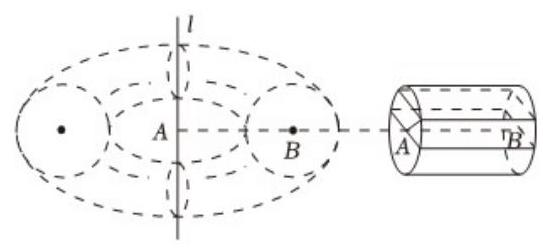
\includegraphics[max width=0.4\textwidth]{images/bo_d5jm9o77aajc7383vmi0_64_294_778_543_248_0.jpg}
\end{center}
\hspace*{3em} 

【答案】 \(1 : {2\pi }\)

【解析】 \({S}_{1} = 2\sqrt{1 - {h}^{2}} \cdot  4 = 8\sqrt{1 - {h}^{2}}\) ,

\begin{center}
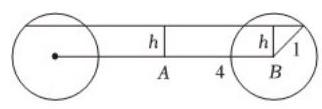
\includegraphics[max width=0.2\textwidth]{images/bo_d5jm9o77aajc7383vmi0_64_1134_1156_322_109_0.jpg}
\end{center}
\hspace*{3em} 

\({S}_{2} = \pi {r}_{\text{ 外 }}^{2} - \pi {r}_{\text{ 内 }}^{2}\) ,其中 \({r}_{\text{ 外 }}^{2} = {\left( 4 + \sqrt{1 - {h}^{2}}\right) }^{2},{r}_{\text{ 内 }}^{2} = {\left( 4 - \sqrt{1 - {h}^{2}}\right) }^{2}\) ,

故 \({S}_{2} = {16}\sqrt{1 - {h}^{2}} \cdot  \pi  = {2\pi }{S}_{1}\) ,即 \(\frac{{S}_{1}}{{S}_{2}} = \frac{1}{2\pi }\) ,

根据祖暅原理, \(T\) 与 \(U\) 的体积之比为 \(1 : {2\pi }\) .

【练习】6. 在 \(\bigtriangleup {ABC}\) 中, \({AB} = 3,{BC} = 4,{AC} = 5,P\) 为 \(\bigtriangleup {ABC}\) 内部一动点 (含边界),在空间中,若到点 \(P\) 的距离不超过 1 的点的轨迹为 \(L\) ，则几何体 \(L\) 的体积等于\_\_\_\_\_.

【答案】 \(\frac{22\pi }{3} + {12}\)

【解析】到动点 \(P\) 距离为 1 的点的轨迹所构成的空间体在垂直于平面 \({ABC}\) 的视角下看,

如图所示,其中 \({BCMN}\text{ 、 }{ACJK}\text{ 、 }{ABYQ}\) 区域内的几何体为半圆柱,

\({CMJ}\text{ 、 }{BNY}\text{ 、 }{KAQ}\) 区域内的几何体为被两平面截的部分球,

球心分别为 \(A\text{ 、 }B\text{ 、 }C,{ABC}\) 区域内的几何体为三棱柱,其高为 2,

因为 \({BCMN}\text{ 、 }{ACJK}\text{ 、 }{ANYQ}\) 为矩形,所以 \(\angle {MCB} = {90}^{ \circ  },\angle {ACJ} = {90}^{ \circ  }\) ,

因为 \(\angle {MCJ} = {360}^{ \circ  } - \left( {\angle {MCB} + \angle {ACJ}}\right)  - \angle {ACB} = {180}^{ \circ  } - \angle {ACB}\) ,

同理, \(\angle {NBY} = {180}^{ \circ  } - \angle {ABC},\angle {KAQ} = {180}^{ \circ  } - \angle {BAC}\) ,

\begin{center}
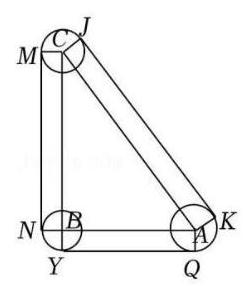
\includegraphics[max width=0.2\textwidth]{images/bo_d5jm9o77aajc7383vmi0_64_1218_1795_246_286_0.jpg}
\end{center}
\hspace*{3em} 

所以 \(\angle {KAQ} + \angle {NBY} + \angle {MCT} = 3 \times  {180}^{ \circ  } - \left( {\angle {ABC} + \angle {BAC} + \angle {ACB}}\right)  = \; {360}^{ \circ  }\) ,

所以这三个区域的几何体合成一个完整的半径为 1 的球,

所以 \({V}_{CMT} + {V}_{NBY} + {V}_{KAQ} = \frac{4}{3}\pi  \times  {1}^{3} = \frac{4\pi }{3}\left( {V}_{CMJ}\right.\) 表示 \({CMJ}\) 区域几何体的体积,

其它以此类推),

\({V}_{BCMN} + {V}_{ACJK} + {V}_{ABYQ} = \left( {\frac{1}{2} \times  \pi  \times  {1}^{2}}\right)  \times  \left( {3 + 4 + 5}\right)  = {6\pi }\)

(其中 \(\frac{1}{2} \times  \pi  \times  {1}^{2}\) 表示半圆底面), \({V}_{ABC} = \frac{1}{2} \times  3 \times  4 \times  2 = {12}\) ,

所以几何体 \(L\) 的体积等于 \(\frac{4\pi }{3} + {6\pi } + {12} = \frac{22\pi }{3} + {12}\) .

【练习】7. 空间给定不共面的 \(A\) 、 \(B\) 、 \(C\) 、 \(D\) 四个点，其中任意两点的距离都不相同，考虑具有如下性质的平面 \(\alpha  : A\text{ 、 }B\text{ 、 }C\text{ 、 }D\) 中有三个点到 \(\alpha\) 的距离相同,另外一个点到 \(\alpha\) 的距离是前三个点到 \(\alpha\) 的距离的 2 倍, 这样的平面的个数是\_\_\_\_\_.

【答案】 32

【解析】首先取 3 个点相等,不相等的那个点有 4 种取法.

然后分 3 个点到平面 \(\alpha\) 的距离相等,有以下 2 种可能性:

 \circled{1} 全同侧，这样的平面有 2 个；

 \circled{2} 不同侧，必然 2 个点在一侧，另1 个点在一侧，1 个点的取法有 3 种，并且平面

过三角形两个点边上的中位线. 考虑不相等的点与单侧点是否同侧有两种可能,

每种情况下都唯一确定一个平面,有 6 个.

所以共有 8 个.

综上,满足条件的这样的平面共有 \(4 \times  8 = {32}\) 个.

\section*{板块三:压轴客观题}

\section*{1. 真题回顾}

【例题】1. (2023 上海春考) 设 \(\overrightarrow{OA},\overrightarrow{OB},\overrightarrow{OC}\) 为空间中三组单位向量,且 \(\overrightarrow{OA} \bot  \overrightarrow{OB},\overrightarrow{OA} \bot  \overrightarrow{OC},\overrightarrow{OB}\) 与 \(\overrightarrow{OC}\) 夹角为 \({60}^{ \circ  },P\) 为空间任意一点,且 \(\left| \overrightarrow{OP}\right|  = 1\) ,满足 \(\left| {\overrightarrow{OP} \cdot  \overrightarrow{OC}}\right|  \leq  \left| {\overrightarrow{OP} \cdot  \overrightarrow{OB}}\right|  \leq  \left| {\overrightarrow{OP} \cdot  \overrightarrow{OA}}\right|\) ,则 \(\left| {\overrightarrow{OP} \cdot  \overrightarrow{OC}}\right|\) 的最大值为\_\_\_\_\_.

【答案】 \(\frac{\sqrt{21}}{7}\)

【解析】法一:建立空间直角坐标系, \(A\left( {0,0,1}\right) ,B\left( {\frac{1}{2},\frac{\sqrt{3}}{2},0}\right) ,C(1,0\) ,

\begin{center}
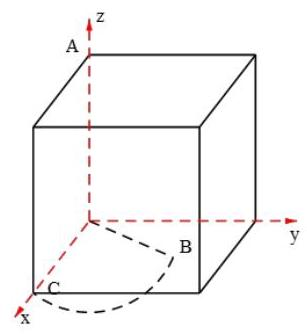
\includegraphics[max width=0.2\textwidth]{images/bo_d5jm9o77aajc7383vmi0_66_1125_621_307_334_0.jpg}
\end{center}
\hspace*{3em} 

\(0)\) ,设 \(P\left( {x,y,z}\right)\) ,则 \({x}^{2} + {y}^{2} + {z}^{2} = 1\) ,

因为 \(\left| {\overrightarrow{OP} \cdot  \overrightarrow{OC}}\right|  \leq  \left| {\overrightarrow{OP} \cdot  \overrightarrow{OB}}\right|  \leq  \left| {\overrightarrow{OP} \cdot  \overrightarrow{OA}}\right|\) ,

所以 \(\left| x\right|  \leq  \left| {\frac{1}{2}x + \frac{\sqrt{3}}{2}y}\right|  \leq  \left| z\right|\) ,

所以 \(x \leq  \frac{1}{2}x + \frac{\sqrt{3}}{2}y \leq  z\) ,

所以 \(\left\{  \begin{array}{l} y \geq  \frac{1}{\sqrt{3}}x \\  x \leq  \frac{1}{2}x + \frac{\sqrt{3}}{2}y \leq  z \end{array}\right.\) ,当且仅当 \(x = \sqrt{3}y = z\) 时取等号;

所以 \(1 = {x}^{2} + {y}^{2} + {z}^{2} \geq  {x}^{2} + {\left( \frac{1}{\sqrt{3}}x\right) }^{2} + {x}^{2}\) ,所以 \({x}^{2} \leq  \frac{3}{7}\) ,

所以 \({\left| \overrightarrow{OP} \cdot  \overrightarrow{OC}\right| }_{\max } = \frac{\sqrt{21}}{7}\) .

法二: 由 \(\left| {\overrightarrow{OP} \cdot  \overrightarrow{OC}}\right|  \leq  \left| {\overrightarrow{OP} \cdot  \overrightarrow{OB}}\right|  \leq  \left| {\overrightarrow{OP} \cdot  \overrightarrow{OA}}\right|\) ,

得 \(\left| {\cos \angle {POC}}\right|  \leq  \left| {\cos \angle {POB}}\right|  \leq  \left| {\cos \angle {POA}}\right|\) ,

由对称性得 \(\angle {POA} = \theta  = \angle {POC} \Rightarrow  \cos \theta  = \cos \left( {\frac{\pi }{2} - \theta }\right)  \cdot  \cos {30}^{ \circ  }\)

所以 \(\tan \theta  = \frac{2}{\sqrt{3}} \Rightarrow  \cos \theta  = \frac{\sqrt{21}}{7} \Rightarrow  {\left| \overrightarrow{OP} \cdot  \overrightarrow{OC}\right| }_{\max } = 1 \times  1 \times  \frac{\sqrt{21}}{7} = \frac{\sqrt{21}}{7}\) .

法三:利用数量积的几何意义

由 \(\left| {\overrightarrow{OP} \cdot  \overrightarrow{OC}}\right|  \leq  \left| {\overrightarrow{OP} \cdot  \overrightarrow{OB}}\right|  \leq  \left| {\overrightarrow{OP} \cdot  \overrightarrow{OA}}\right|\) ,则 \({\left| \overrightarrow{OP} \cdot  \overrightarrow{OC}\right| }_{\max } \leq  \left| {\overrightarrow{OP} \cdot  \overrightarrow{OB}}\right|  \leq  \left| {\overrightarrow{OP} \cdot  \overrightarrow{OA}}\right|\) ,

由数量积的几何意义,易得当且仅当 \({OP} \bot\) 面 \({ABC}\) 时取等号,

不妨设点 \(O\) 到平面 \({ABC}\) 的距离为 \(h\) ，则 \({V}_{O - {ABC}} = {V}_{A - {OBC}}\) ，得 \(h = \frac{\sqrt{21}}{7}\) ，

即 \({\left| \overrightarrow{OP} \cdot  \overrightarrow{OC}\right| }_{\max } = h = \frac{\sqrt{21}}{7}\) .

法四:利用三余弦定理求解，

由题意得 \(\left| \overrightarrow{OA}\right|  = \left| \overrightarrow{OB}\right|  = \left| \overrightarrow{OC}\right|  = \left| \overrightarrow{OP}\right|  = 1\) ,

不妨设 \(< \overrightarrow{OP},\overrightarrow{OA} >  = {\theta }_{1}, < \overrightarrow{OP},\overrightarrow{OB} >  = {\theta }_{2}, < \overrightarrow{OP},\overrightarrow{OC} >  = {\theta }_{3}\) ,

\begin{center}
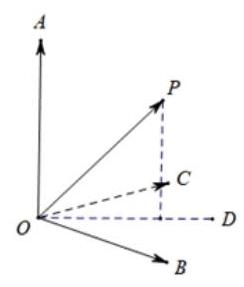
\includegraphics[max width=0.2\textwidth]{images/bo_d5jm9o77aajc7383vmi0_66_1201_1813_244_287_0.jpg}
\end{center}
\hspace*{3em} 

记直线 \({OP}\) 与平面 \({OBC}\) 所成角为 \(\theta\) ,

又 \(\left| {\overrightarrow{OP} \cdot  \overrightarrow{OC}}\right|  \leq  \left| {\overrightarrow{OP} \cdot  \overrightarrow{OB}}\right|  \leq  \left| {\overrightarrow{OP} \cdot  \overrightarrow{OA}}\right|\) ,可化为 \(\left| {\cos {\theta }_{3}}\right|  \leq  \left| {\cos {\theta }_{2}}\right|  \leq  \left| {\cos {\theta }_{1}}\right|\) ,

题目求 \(\left| {\overrightarrow{OP} \cdot  \overrightarrow{OC}}\right|\) 的最大值,即是求 \(\left| {\cos {\theta }_{3}}\right|\) 的最大值,

即 \({\left| \cos {\theta }_{3}\right| }_{\max } \leq  \left| {\cos {\theta }_{2}}\right|  \leq  \left| {\cos {\theta }_{1}}\right|\) ,下面探索何时取等号,

由三垂线定理得 \(\left\{  \begin{array}{l} {\theta }_{1} = {\theta }_{2} = {\theta }_{3} \\  {\theta }_{1} + \theta  = {90}^{ \circ  } \\  \cos {\theta }_{2} = \cos \theta \cos {30}^{ \circ  } \end{array}\right.\) ,解得 \(\left| {\cos {\theta }_{3}}\right|  = \frac{\sqrt{21}}{7}\) ,

综上, \({\left| \overrightarrow{OP} \cdot  \overrightarrow{OC}\right| }_{\max } = \frac{\sqrt{21}}{7}\) .

法五:一撸到底+线性规划，

建立空间直角坐标系,设 \(B\left( {1,0,0}\right) ,A\left( {0,0,1}\right) ,C\left( {\frac{1}{2},\frac{\sqrt{3}}{2},0}\right) ,P\left( {x,y,z}\right)\) .

所以 \(\left| {\overrightarrow{OP} \cdot  \overrightarrow{OC}}\right|  = \left| {\frac{1}{2}x + \frac{\sqrt{3}}{2}y}\right| ,\left| {\overrightarrow{OP} \cdot  \overrightarrow{OB}}\right|  = \left| x\right| ,\left| {\overrightarrow{OP} \cdot  \overrightarrow{OA}}\right|  = \left| z\right|\) ,

当 \(x \geq  0\) 时,有 \(- x \leq  \frac{1}{2}x + \frac{\sqrt{3}}{2}y \leq  x\) ,得 \(- \sqrt{3}x \leq  y \leq  \frac{\sqrt{3}}{3}x\) ;

当 \(x < 0\) 时,有 \(x \leq  \frac{1}{2}x + \frac{\sqrt{3}}{2}y \leq   - x\) ,得 \(\frac{\sqrt{3}}{3}x \leq  y \leq   - \sqrt{3}x\) ;

设 \(z = \frac{1}{2}x + \frac{\sqrt{3}}{2}y\) ,即 \(y = \frac{2}{\sqrt{3}}z - \frac{x}{\sqrt{3}}\) ,

在边界, \(z\) 会有最大值和最小值,且为相反数.

由 \(\left\{  \begin{array}{l} 2{x}^{2} + {y}^{2} = 1 \\  y = \frac{\sqrt{3}}{3}x \end{array}\right.\) ,得 \(x = \frac{\sqrt{21}}{7},y = \frac{\sqrt{7}}{7}\) ,所以 \({z}_{E} = \frac{\sqrt{21}}{7}\) ,

所以 \(z \in  \left\lbrack  {-\frac{\sqrt{21}}{7},\frac{\sqrt{21}}{7}}\right\rbrack\) ,故 \({z}_{\max } = \frac{\sqrt{21}}{7}\) .

法六:在法五的基础上，利用取等条件对思路一进行优化，可省去线性规划的过程因为 \(\left| \overrightarrow{OP}\right|\) .

\(\left| \overrightarrow{OC}\right|  \leq  \left| {\overrightarrow{OP} \cdot  \overrightarrow{OB}}\right|  \leq  \left| {\overrightarrow{OP} \cdot  \overrightarrow{OA}}\right| ,\)

所以当 \(\left| {\overrightarrow{OP} \cdot  \overrightarrow{OC}}\right|\) 取得最大,则必有 \(\left| {\overrightarrow{OP} \cdot  \overrightarrow{OC}}\right|  = \left| {\overrightarrow{OP} \cdot  \overrightarrow{OB}}\right|  = \left| {\overrightarrow{OP} \cdot  \overrightarrow{OA}}\right|\) ,

建立空间直角坐标系,设 \(B\left( {1,0,0}\right) ,A\left( {0,0,1}\right) ,C\left( {\frac{1}{2},\frac{\sqrt{3}}{2},0}\right) ,P\left( {x,y,z}\right)\) .

所以有 \(\left| {\overrightarrow{OP} \cdot  \overrightarrow{OC}}\right|  = \left| {\frac{1}{2}x + \frac{\sqrt{3}}{2}y}\right| ,\left| {\overrightarrow{OP} \cdot  \overrightarrow{OB}}\right|  = \left| x\right| ,\left| {\overrightarrow{OP} \cdot  \overrightarrow{OA}}\right|  = \left| z\right|\) ,

进而有 \(\left| {\frac{1}{2}x + \frac{\sqrt{3}}{2}y}\right|  = \left| x\right|  = \left| z\right|\)  \circled{1} ,

由球面的对称性, \(P\) 在 \({xOy}\) 面上下是等价的,去上面四个卦限研究;

\(P\) 在第一卦限和第三卦限等价,第二卦限和第四卦限等价,

且第一卦限比第二卦限优越,所以最终可以将 \(P\) 等价在第一卦限,

故 \(x > 0,y > 0,z > 0\) ,

所以有 \(\left\{  \begin{array}{l} \frac{1}{2}x + \frac{\sqrt{3}}{2}y = x \\  x = z \\  {x}^{2} + {y}^{2} + {z}^{2} = 1 \end{array}\right.\) ,解得 \(\left\{  \begin{array}{l} x = \frac{\sqrt{21}}{7} \\  y = \frac{\sqrt{7}}{7} \end{array}\right.\) ,得 \({\left| \overrightarrow{OP} \cdot  \overrightarrow{OC}\right| }_{\max } = \frac{\sqrt{21}}{7}\) .

法七:利用空间解析几何面的方程，

由 \(\left| {\overrightarrow{OP} \cdot  \overrightarrow{OB}}\right|  \leq  \left| {\overrightarrow{OP} \cdot  \overrightarrow{OA}}\right|\) ,得 \(P\) 在 \(\angle {AOB}\) 的角平分面上侧及含面内,

面的方程为 \(x - z = 0\) ;

由 \(\left| {{OP} \cdot  \overrightarrow{OC}}\right|  \leq  \left| {\overrightarrow{OP} \cdot  \overrightarrow{OB}}\right|\) ,得 \(P\) 在 \(\angle {COB}\) 的角平分面左侧及含面内,

面的方程为 \(x - \sqrt{3}y = 0\) ;

2025 版上海高考真题及模拟训练合集(下册)

想 \(\left| {\overrightarrow{OP} \cdot  \overrightarrow{OC}}\right|\) 取得最大,必有 \(\left\{  \begin{array}{l} x - \sqrt{3}y = 0 \\  x = z \end{array}\right.\) ,解得 \(\left\{  \begin{array}{l} x = \frac{\sqrt{21}}{7} \\  y = \frac{\sqrt{7}}{7} \\  z = \frac{\sqrt{21}}{7} \end{array}\right.\) ,

得 \({\left| \overrightarrow{OP} \cdot  \overrightarrow{OC}\right| }_{\max } = \frac{\sqrt{21}}{7}\) .

【例题】2. (2023 上海秋考) 已知空间中存在三点 \(A\text{ 、 }B\text{ 、 }C\) ,且 \({AB} = {AC} = {BC} = 1\) . 若从空间中再任取不同的两点 (不计顺序), 使得这五点构成一个正四棱锥, 则不同的取法共有\_\_\_\_\_种.

【答案】 9

【解析】法一:

\begin{center}
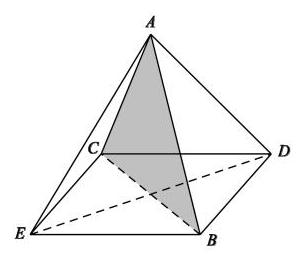
\includegraphics[max width=0.2\textwidth]{images/bo_d5jm9o77aajc7383vmi0_68_307_716_298_254_0.jpg}
\end{center}
\hspace*{3em} 

\begin{center}
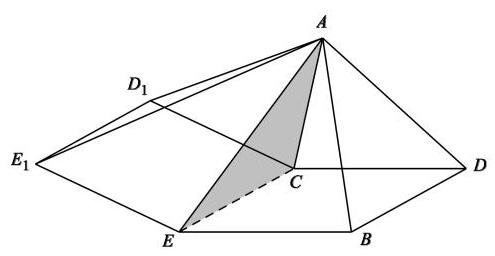
\includegraphics[max width=0.4\textwidth]{images/bo_d5jm9o77aajc7383vmi0_68_635_711_495_256_0.jpg}
\end{center}
\hspace*{3em} 

\({1}^{ \circ  }\) 若以平面 \({ABC}\) 为正四棱锥的一个侧面时,

在其两侧分别可以作以 \({BC}\) 为一边的正方形 \({BCDE}\) 或 \({BC}{D}_{1}{E}_{1}\) ,

这样的四棱锥共 2 种,

同理,以 \({AB}\text{ 、 }{AC}\) 为底面正方形一边的四棱锥也各有 2 种,

所以,这样的四棱锥共 \(2 + 2 + 2 = 6\) 种;

\({2}^{ \circ  }\) 若以平面 \({ABC}\) 为正四棱锥的一个对角面时,

此时 \({DE}\) 只能为底面正方形的另一条对角线,

同理, \({AB}\text{ 、 }{AC}\) 为底面正方形一条对角线时, \({DE}\) 的位置情况,也各一种,

这样共 3 种;

综上,满足题意的四棱锥共 \(6 + 3 = 9\) 种.

法二:首先， \(\bigtriangleup  {ABC}\) 为等边三角形，

则取的两点 \(D,E\) 都不可能作为正方形外的顶点,

否则若 \(D\) 为顶点,则 \(A,B,C,E\) 需要组成正方形,这不可能.

\begin{center}
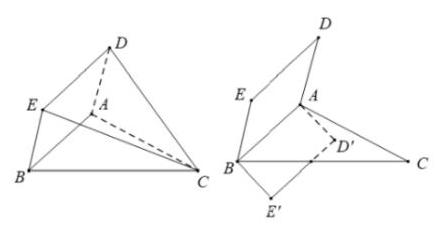
\includegraphics[max width=0.3\textwidth]{images/bo_d5jm9o77aajc7383vmi0_68_1014_1585_436_225_0.jpg}
\end{center}
\hspace*{3em} 

所以只能 \(A,B,C\) 作为顶点,下面只需讨论 \(C\) 为顶点时即可,

不失一般性,所得结果乘以 3 即为最终结果.

当 \(C\) 为顶点时,

 \circled{1}  \({AB}\) 为正方形的边，则正方形 \({ABDE}\) 可以

在平面 \({ABC}\) 的斜上方或斜下方,

\begin{center}
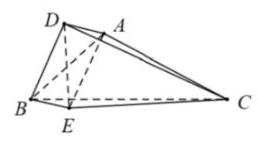
\includegraphics[max width=0.2\textwidth]{images/bo_d5jm9o77aajc7383vmi0_68_1189_1849_258_141_0.jpg}
\end{center}
\hspace*{3em} 

两种情况关于平面 \({ABC}\) 对称，共 2 个；

 \circled{2}  \({AB}\) 为正方形的对角线，点 \(D\) ， \(E\) 出现在 \({AB}\) 的正上方和正下方，

即正方形 \({ADBE} \bot\) 平面 \({ABC}\) ,共 1 个;

综上,共有 \(\left( {2 + 1}\right)  \times  3 = 9\) 个.

【例题】3. (2012上海秋考)如图， \({AD}\) 与 \({BC}\) 是四面体 \({ABCD}\) 中互相垂直的棱， \({BC} = 2\) ，若 \({AD} = {2c}\) ，且

\begin{center}
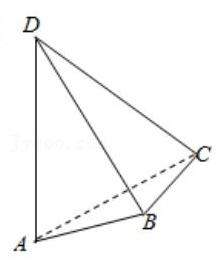
\includegraphics[max width=0.2\textwidth]{images/bo_d5jm9o77aajc7383vmi0_69_1231_230_219_262_0.jpg}
\end{center}
\hspace*{3em} 

\({AB} + {BD} = {AC} + {CD} = {2a}\) ，其中 \(a\) 、 \(c\) 为常数，则四面体 \({ABCD}\) 的体积的最大

值是\_\_\_\_\_.

【答案】 \(\frac{2}{3}c\sqrt{{a}^{2} - {c}^{2} - 1}\)

【解析】作 \({BE} \bot  {AD}\) 于 \(E\) ,连接 \({CE}\) ,则 \({AD} \bot\) 平面 \({BEC}\) ,所以 \({CE} \bot  {AD}\) ,

由题意得 \(B\) 与 \(C\) 都是在以 \({AD}\) 为焦点的椭球上,

且 \({BE}\text{ 、 }{CE}\) 都垂直于焦距 \({AD}\) ,

\({AB} + {BD} = {AC} + {CD} = {2a}\) ,显然 \(\bigtriangleup {ABD} \cong  \bigtriangleup {ACD}\) ,所以 \({BE} = {CE}\) .

取 \({BC}\) 中点 \(F\) ，所以 \({EF}\bot {BC},{EF}\bot {AD}\) ，

\begin{center}
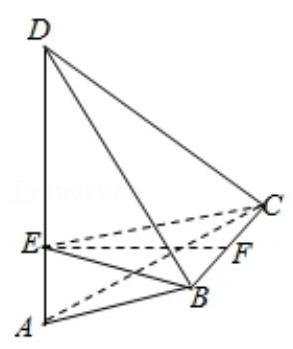
\includegraphics[max width=0.2\textwidth]{images/bo_d5jm9o77aajc7383vmi0_69_1161_601_293_349_0.jpg}
\end{center}
\hspace*{3em} 

要求四面体 \({ABCD}\) 的体积的最大值，

因为 \({AD}\) 是定值，只需三角形 \({EBC}\) 的面积最大，

因为 \({BC}\) 是定值，所以只需 \({EF}\) 最大即可，

当 \(\bigtriangleup {ABD}\) 是等腰三角形时几何体的体积最大,

因为 \({AB} + {BD} = {AC} + {CD} = {2a}\) ，所以 \({AB} = a\) ，

所以 \({EB} = \sqrt{{a}^{2} - {c}^{2}},{EF} = \sqrt{{a}^{2} - {c}^{2} - 1}\) ，

所以几何体的体积为 \(\frac{1}{3} \times  2 \times  \sqrt{{a}^{2} - {c}^{2} - 1} \times  {2c} \times  \frac{1}{2} =\)

\(\frac{2}{3}c\sqrt{{a}^{2} - {c}^{2} - 1}\) 2025 版上海高考真题及模拟训练合集(下册)

\section*{2. 模拟练习}

【练习】1. (2025 届华二) 设 \({A}_{1},{B}_{1},{C}_{1},{D}_{1}\) 分别是四棱锥 \(P - {ABCD}\) 侧棱 \({PA},{PB},{PC},{PD}\) 上的点. 给出以下两个命题, 则 ( )

 \circled{1} 若 \({ABCD}\) 是平行四边形，但不是菱形，则 \({A}_{1}{B}_{1}{C}_{1}{D}_{1}\) 可能是菱形;

 \circled{2} 若 \({ABCD}\) 不是平行四边形,则 \({A}_{1}{B}_{1}{C}_{1}{D}_{1}\) 可能是平行四边形.

A.  \circled{1} 真 \circled{2} 真 B.  \circled{1} 真 \circled{2} 假 C.  \circled{1} 假 \circled{2} 真 D.  \circled{1} 假 \circled{2} 假

【答案】 \(C\)

【解析】对于 \circled{2} , 考虑一个正四棱锥, 然后在他的侧棱的延长线上可以画出一个梯形, 具体做法是: 取 \(P{A}_{1} = P{B}_{1} = P{C}_{1} = P{D}_{1}\) ,

\begin{center}
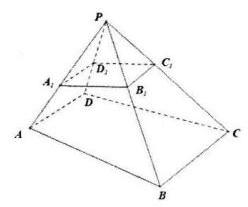
\includegraphics[max width=0.2\textwidth]{images/bo_d5jm9o77aajc7383vmi0_70_296_665_248_207_0.jpg}
\end{center}
\hspace*{3em} 

则四棱锥 \(P - {A}_{1}{B}_{1}{C}_{1}{D}_{1}\) 为正四棱锥,

然后令 \({PA} = {2P}{A}_{1},{PB} = {2P}{B}_{1},{PC} = {3P}{C}_{1},{PD} = {3P}{D}_{1}\) ,

那么 \({AD}//{BC},{AD} \neq  {BC}\) ,此时 \({ABCD}\) 是梯形,但不是平行四边形;

对于 \circled{1} ，如图，四边形 \({ABCD}\) 为平行四边形， \({A}_{1}{B}_{1}{C}_{1}{D}_{1}\) 也为平行四边形，

若平面 \({ABCD}\) 与平面 \({A}_{1}{B}_{1}{C}_{1}{D}_{1}\) 不平行，

\begin{center}
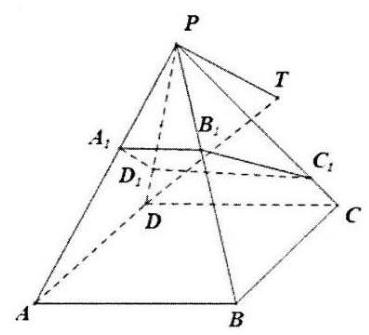
\includegraphics[max width=0.3\textwidth]{images/bo_d5jm9o77aajc7383vmi0_70_293_1111_369_335_0.jpg}
\end{center}
\hspace*{3em} 

则四边形 \({A}_{1}{B}_{1}{C}_{1}{D}_{1}\) 中必有一边与底面 \({ABCD}\) 相交,

不妨设直线 \({A}_{1}{D}_{1}\) 与底面相交,则直线 \({B}_{1}{C}_{1}\) 也与底面相交,

在平面 \({PAD}\) 中过 \(P\) 作 \({A}_{1}{D}_{1}\) 的平行线,交 \({AD}\) 与 \(T\) ,则 \({PT}//{B}_{1}{C}_{1}\) ,

而 \(P \in\) 平面 \({PBC},{B}_{1}{C}_{1} \subset\) 平面 \({PBC}\) ,故 \({PT} \subset\) 平面 \({PBC}\) ,即 \(T \in\) 平面 \({PBC}\) ,

而平面 \({PBC} \cap\) 平面 \({ABCD} = {BC}\) ,故 \(T \in  {BC}\) ,而 \(T \in  {AD}\) ,

故 \({BC},{AD}\) 相交,这与 \({ABCD}\) 为平行四边形矛盾.

故平面 \({ABCD}//\) 平面 \({A}_{1}{B}_{1}{C}_{1}{D}_{1}\) ,故 \(\frac{{A}_{1}{B}_{1}}{AB} = \frac{P{A}_{1}}{PA} = \frac{{A}_{1}{D}_{1}}{AD}\) ,

若四边形 \({A}_{1}{B}_{1}{C}_{1}{D}_{1}\) 为菱形,则 \({A}_{1}{B}_{1} = {A}_{1}{D}_{1}\) ,则 \({AB} = {AD}\) ,

故四边形 \({ABCD}\) 为菱形,故 \circled{1} 错误.

故选 \(C\) .

【练习】2. (2024 届华二) 设 \({l}_{1}\text{ 、 }{l}_{2}\text{ 、 }{l}_{3}\) 为空间中三条互相平行且两两间的距离分别为4,5,6的直线.

给出下列两个结论:  \circled{1} 存在 \({A}_{i} \in  {l}_{i}\left( {\mathrm{i} = 1,2,3}\right)\) ,使得 \(\bigtriangleup {A}_{1}{A}_{2}{A}_{3}\) 是钝角三角形;  \circled{2} 存在 \({A}_{i} \in\)

\({l}_{i}\left( {\mathrm{i} = 1,2,3}\right)\) ,使得 \(\bigtriangleup {A}_{1}{A}_{2}{A}_{3}\) 是等边三角形; 则下列正确的是 ( ) 2025 版上海高考真题及模拟训练合集(下册)

A.  \circled{1} 成立 \circled{2} 成立 B.  \circled{1} 成立 \circled{2} 不成立

C.  \circled{1} 不成立 \circled{2} 成立 D.  \circled{1} 不成立 \circled{2} 不成立

【答案】 \(A\)

【解析】我们不妨先将 \(A\text{ 、 }B\text{ 、 }C\) 按如图所示放置.

\begin{center}
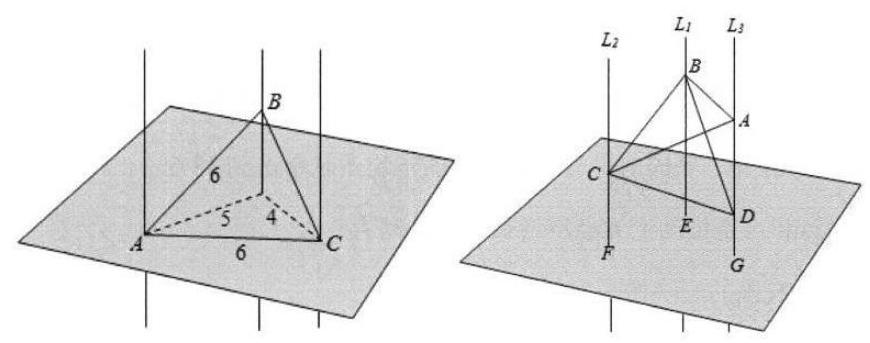
\includegraphics[max width=0.7\textwidth]{images/bo_d5jm9o77aajc7383vmi0_71_305_430_870_343_0.jpg}
\end{center}
\hspace*{3em} 

容易看出此时 \({BC} < {AB} = {AC}\) .

现在，我们将 \(A\) 和 \(B\) 往上移，并且总保持 \({AB} = {AC}\) (这是可以做到的，

只要 \(A\) 、 \(B\) 的速度满足一定关系)，

而当 \(A\) 、 \(B\) 移得很高很高时，不难想象 \(\bigtriangleup  {ABC}\) 将会变得很扁，

也就是会变成顶角 \(A\) “非常钝” 的一个等腰钝角三角形.

于是，在移动过程中，总有一刻，使 \(\bigtriangleup  {ABC}\) 成为等边三角形，

亦总有另一刻，使 \(\bigtriangleup  {ABC}\) 成为直角三角形 (而且还是等腰的).

这样,就得到 \circled{1} 和 \circled{2} 都是正确的. 故选 \(A\) .

【练习】3. (2026 届复附)光线沿直线 \(l\) 以 \({30}^{ \circ  }\) 的入射角 (指入射光线与入射表面法线的夹角) 照射到镜面 \(\alpha\) 上的点 \(A\) ，反射光线为射线 \({AB}\) ， \(l\) 在平面 \(\alpha\) 上的射影为 \({l}^{\prime }\) ，现将镜面以 \({l}^{\prime }\) 为轴旋转 \({45}^{ \circ  }\) ，反射光线变为射线 \({AC}\) ，则 \(\angle {BAC}\) 的大小为\_\_\_\_\_.

【答案】 \(\arccos \frac{1}{4}\)

【解析】在长方体中, \({DA}\) 表示入射线,平面 \({EFA}\) 为平面 \(\alpha ,{DA}\) 在平面 \(\alpha\) 的射影为 \({FA}\) ,因为直线 \({DA}\) 照射到平面 \(\alpha\) 的入射角为 \({30}^{ \circ  }\) ,所以 \(\angle {DAF} = {60}^{ \circ  }\) .

\begin{center}
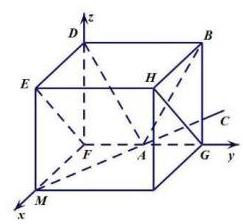
\includegraphics[max width=0.2\textwidth]{images/bo_d5jm9o77aajc7383vmi0_71_1220_1459_243_224_0.jpg}
\end{center}
\hspace*{3em} 

不妨令 \({FD} = {FM} = \sqrt{3},{FA} = 1\) ,

将平面 \(\alpha\) 绕 \({FA}\) 轴旋转 \({45}^{ \circ  }\) 得平面 \({EFGH}\) ,

则 \(A\left( {0,1,0}\right)\) ,可取 \(B\left( {0,2,\sqrt{3}}\right)\) ,

则反射光线 \({AB}\) 的方向向量为 \(\overrightarrow{AB} = \left( {0,1,\sqrt{3}}\right)\) .

因为点 \(D\) 关于平面 \({EFGH}\) 的对称点为 \(M\left( {\sqrt{3},0,0}\right)\) ,

所以反射线 \({AC}\) 的方向向量为 \(\overrightarrow{MA} = \left( {-\sqrt{3},1,0}\right)\) ,

所以 \(\cos \angle {BAC} = \frac{\overrightarrow{AB} \cdot  \overrightarrow{MA}}{\left| \overrightarrow{AB}\right|  \cdot  \left| \overrightarrow{MA}\right| } = \frac{1}{2 \times  2} = \frac{1}{4}\) ，所以 \(\angle {BAC} = \arccos \frac{1}{4}\) .

【练习】4. 已知异面直线 \(a\text{ 、 }b\) 所成角为 \({60}^{ \circ  }\) ,直线 \({AB}\) 与 \(a\text{ 、 }b\) 均垂直,且垂足分别是点 \(A\text{ 、 }B\) ,若动点 \(P \in \; a,Q \in  b,\left| {PA}\right|  + \left| {QB}\right|  = m\) ，则线段 \({PQ}\) 中点 \(M\) 的轨迹围成的区域的面积是\_\_\_\_\_.

【答案】 \(\frac{\sqrt{3}{m}^{2}}{4}\)

【解析】设线段 \({AB}\) 的中垂面为 \(\alpha\) ,则 \(M\) 的轨迹在平面 \(\alpha\) 内,

在平面 \(\alpha\) 内分别作直线 \(a\text{ 、 }b\) 的投影 \({a}^{\prime }\text{ 、 }{b}^{\prime }\) ,则两直线的夹角为 \({60}^{ \circ  }\) ,

设 \(A\text{ 、 }B\) 在平面 \(\alpha\) 的投影为 \(O,P\text{ 、 }Q\) 在平面 \(\alpha\) 内的投影分别为 \({P}^{\prime }\text{ 、 }{Q}^{\prime }\) ,

则 \(M\) 为 \({P}^{\prime }{Q}^{\prime }\) 的中点，所以 \(O{P}^{\prime } = {PA},O{Q}^{\prime } = {BQ}\) ，

因为 \(\left| {PA}\right|  + \left| {QB}\right|  = m\) ，所以 \(O{P}^{\prime } + O{Q}^{\prime } = m\) .

在直线 \({a}^{\prime }\text{ 、 }{b}^{\prime }\) 上分别取点 \(E\text{ 、 }F\text{ 、 }G\text{ 、 }H\) 四点,

\begin{center}
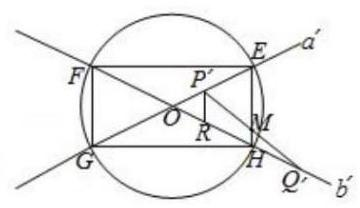
\includegraphics[max width=0.3\textwidth]{images/bo_d5jm9o77aajc7383vmi0_72_1099_423_360_208_0.jpg}
\end{center}
\hspace*{3em} 

使得 \({OE} = {OF} = {OG} = {OH} = \frac{m}{2}\) ,

因为 \({OE} + {OH} = {O{P}^{\prime }} + {O{Q}^{\prime }} = m\) ，所以 \({{P}^{\prime }E} = {H{Q}^{\prime }}\) ，

过 \({P}^{\prime }\) 作 \({P}^{\prime }R//{EH}\) 交 \(O{Q}^{\prime }\) 于 \(R\) ,则 \({HR} = {P}^{\prime }E = H{Q}^{\prime }\) ,

所以 \({P}^{\prime }{Q}^{\prime }\) 的中点 \(M\) 在 \({EH}\) 上,同理可得 \(M\) 在 \({EF}\text{ 、 }{FG}\text{ 、 }{GH}\) 上,所

以 \(M\) 的轨迹为矩形 \({EHGH}\) .

因为 \(\angle {EOH} = {60}^{ \circ  },{OE} = {OF} = {OG} = {OH} = \frac{m}{2}\) ,

所以 \({S}_{\text{ 矩形 }{EFGH}} = \frac{1}{2} \times  \frac{m}{2} \times  \frac{m}{2} \times  \sin {60}^{ \circ  } \times  2 + \frac{1}{2} \times  \frac{m}{2} \times  \frac{m}{2} \times  \sin {120}^{ \circ  } \times  2 = \frac{\sqrt{3}{m}^{2}}{4}\) .

【练习】5. (2024 届华二) 点 \(O\) 是正四面体 \({A}_{1}{A}_{2}{A}_{3}{A}_{4}\) 的中心, \(\left| {O{A}_{i}}\right|  = 1\left( {\mathrm{i} = 1,2,3,4}\right)\) .

若 \(\overrightarrow{OP} = {\lambda }_{1}\overrightarrow{O{A}_{1}} + {\lambda }_{2}\overrightarrow{O{A}_{2}} + {\lambda }_{3}\overrightarrow{O{A}_{3}} + {\lambda }_{4}\overrightarrow{O{A}_{4}}\) ,其中 \(0 \leq  {\lambda }_{i} \leq  1\left( {\mathrm{i} = 1,2,3,4}\right)\) ,则动点 \(P\) 扫过的区域的体积为\_\_\_\_\_.

【答案】 \(\frac{{16}\sqrt{3}}{9}\)

【解析】本题较为复杂,考虑 \({\lambda }_{i}\) 取 0 到 1 的端点值,

\begin{center}
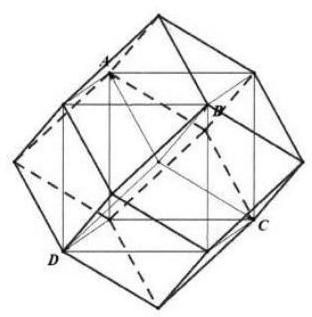
\includegraphics[max width=0.2\textwidth]{images/bo_d5jm9o77aajc7383vmi0_72_329_1078_312_317_0.jpg}
\end{center}
\hspace*{3em} 

考虑两个 \({\lambda }_{i}\) 取 1,其余两个取 0 ; 考虑三个 \({\lambda }_{i}\) 取 1,其余 1 个取 0 ;

把该四面体嵌入正方体中作图，

所求体积为两倍的正方体，计算得 \(\frac{{16}\sqrt{3}}{9}\) .

【练习】6. 已知棱长均为 1 的正 \(n\) 棱柱有 \({2n}\) 个顶点,从中任取两个顶点作为向量 \(\overrightarrow{a}\) 的起点与终点,设底面的一条棱为 \({AB}\) . 若集合 \({A}_{n} = \{ x \mid  x = \overrightarrow{a} \cdot  \overrightarrow{AB}\}\) ,则当 \({A}_{n}\) 中的元素个数最少时, \(n\) 的值为 ( )

A. 3 B. 4 C. 6 D. 8

【答案】 \(B\)

【解析】因为 \(\overrightarrow{a}\) 都可以表示成正 \(n\) 棱柱底面顶点连线对应向量的和向量,

或底面向量与垂直于底面的向量的和向量,

由数量积的运算律得 \(\overrightarrow{a} \cdot  \overrightarrow{AB}\) 可化为底面中任意两顶点连线对应向量与 \(\overrightarrow{AB}\) 的

数量积,

再由数量积的几何意义得,当底面所有任意两点连线对应向量在 \(\overrightarrow{AB}\) 上投影向量个数最少时,

对应的 \(n\) 值即为所求,

显然正方形 \({ABCD}\) 中,取 \(\overrightarrow{AB}\) ,其余任意两点连线对应向量在 \(\overrightarrow{AB}\) 上的投影向量

只有 \(\overrightarrow{0}\) (与 \(\overrightarrow{AB}\) 垂直的向量的投影向量),

以及 \(\overrightarrow{AB}\) 同向的相等向量或反向的相反向量 \(\overrightarrow{BA}\) 两种情况,

则最终 \(x\) 的值有 \(0, \pm  {\left| AB\right| }^{2} =  \pm  1\) ,此时 \(x = 3\) ;

同理, \(n = 3\) 时, \(x\) 的值为 4 ; 当 \(n = 5,6,\cdots \cdots ,x\) 的值必然大于 3,

当 \({A}_{n}\) 中的元素个数最少时, \(n\) 的值为 4 .

故选 B.

【练习】7. 设四面体 \({ABCD}\) 中,有 \(k\) 条棱长为 \(a\) ,其余 \(6 - k\) 条棱长为 1 .

(1) \(k = 1\) 时，求 \(a\) 的取值范围；

(2) \(k = 2\) 时，求 \(a\) 的取值范围.

【解析】(1) 设 \({AB} = a\) ，固定 \(\bigtriangleup  {BCD}\) ，让 \(\bigtriangleup  {ACD}\) 绕 \({CD}\) 转动，

\begin{center}
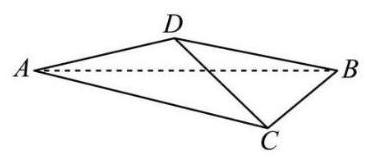
\includegraphics[max width=0.3\textwidth]{images/bo_d5jm9o77aajc7383vmi0_73_1092_808_365_159_0.jpg}
\end{center}
\hspace*{3em} 

当 \(A\) 接近 \(B\) 时， \(a\) 接近于 0 ；

当 \(\bigtriangleup  {ACD}\) 与 \(\bigtriangleup  {BCD}\) 接近于共面时， \(a\) 接近于 \(\sqrt{3}\) ；

故 \(a \in  \left( {0,\sqrt{3}}\right)\) ；

(2)第一种情况，两边在一个三角形内时:

假设 \({AB} = {AC} = a > 0,{DA} = {DB} = {DC} = {BC} = 1\) 时， \(E\) 为 \(D\) 在底面射影，

由题意得 \({EA} = {EB} = {EC}\) ，假设 \({BC}\) 中点为 \(O\) ，连结 \({EO}\) ，

假设 \({EA} = {EC} = x < 1\) ,则 \({EO} = \sqrt{{x}^{2} - \frac{1}{4}},{AO} = x + \sqrt{{x}^{2} - \frac{1}{4}},A \ll\)

\begin{center}
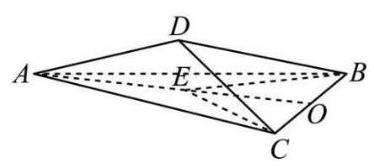
\includegraphics[max width=0.3\textwidth]{images/bo_d5jm9o77aajc7383vmi0_73_1089_1151_374_166_0.jpg}
\end{center}
\hspace*{3em} 

\(A{O}^{2} + C{O}^{2} = A{C}^{2}\) ,即 \({\left( x + \sqrt{{x}^{2} - \frac{1}{4}}\right) }^{2} + \frac{1}{4} = {a}^{2}\) ,

解得 \(\left\{  \begin{array}{l} {a}^{4} = \left( {4{a}^{2} - 1}\right) {x}^{2} \\  4{a}^{2} - 1 > 0 \end{array}\right.\) ,则 \(x = \frac{{a}^{2}}{\sqrt{4{a}^{2} - 1}} < 1\) 且 \(a > \frac{1}{2}\) ,

即 \({a}^{4} - 4{a}^{2} + 1 < 0\) ,故 \(2 - \sqrt{3} < {a}^{2} < 2 + \sqrt{3}\) ,则 \(\frac{\sqrt{6} - \sqrt{2}}{2} < a <\)

\(\frac{\sqrt{6} + \sqrt{2}}{2}\) ,

综上, \(\frac{\sqrt{6} - \sqrt{2}}{2} < a < \frac{\sqrt{6} + \sqrt{2}}{2}\) ;

第二种情况，两边不在一个三角形内时:

假设 \({AC} = {BD} = a,{AB} = {AD} = {CB} = {CD} = 1\) ,

发现当等腰三角形两腰的夹角接近 \({0}^{ \circ  }\) 时, \(a\) 在减小但总是存在的,故 \(a > 0\) ,

假设 \({AC} = {BD} = a,{AB} = {AD} = {CB} = {CD} = 1\) ,取 \({AC}\) 中点 \(G\) ,

连接 \({DG}\text{ 、 }{BG}\) ,则 \({DG} = {BG} = \sqrt{1 - \frac{{a}^{2}}{4}}\) ,

\begin{center}
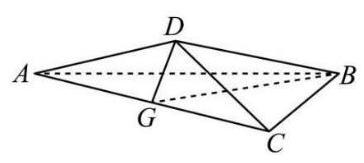
\includegraphics[max width=0.3\textwidth]{images/bo_d5jm9o77aajc7383vmi0_73_1095_1775_364_163_0.jpg}
\end{center}
\hspace*{3em} 

由两边之和大于第三边得 \(2\sqrt{1 - \frac{{a}^{2}}{4}} > a\) ,解得 \(a < \sqrt{2}\) ,故 \(a \in \; \left( {0,\sqrt{2}}\right)\) ,

综上, \(a \in  \left( {0,\frac{\sqrt{6} + \sqrt{2}}{2}}\right)\) .

\section*{板块四: 基础主观题}

\section*{1. 真题回顾}

\begin{center}
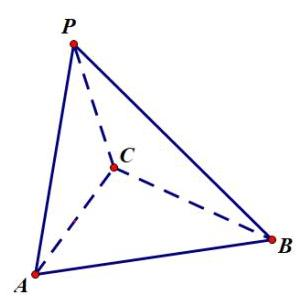
\includegraphics[max width=0.2\textwidth]{images/bo_d5jm9o77aajc7383vmi0_74_1121_361_301_301_0.jpg}
\end{center}
\hspace*{3em} 

【例题】1. (2025 上海春考) 已知三棱锥 \(P - {ABC}\) ，平面 \({ABC} \bot\) 平面 \({PAC},{PA} = {AC} = {PC} = 2,{AB} = {BC} = \sqrt{2}.\)

(1)设 \({AC}\) 中点为 \(O\) ，求证: \({BO}\bot\) 平面 \({PAC}\) ，并求三棱锥 \(B - \; {PAO}\) 的体积；

(2) 求二面角 \(B - {PC} - A\) 的大小.

【解析】(1) 连 \({PO}\) ,则 \({BO} \bot  {AC}\) .

又 \({PO} \bot  {AC}\) ,所以 \(\angle {POB}\) 为 \(P - {AC} - B\) 的平面角,即 \(\angle {POB} = \; {90}^{ \circ  }\) ,所以 \({BO} \bot  {PO}\) .

又 \({PO} \cap  {AC} = O\) ,所以 \({BO} \bot\) 平面 \({PAC}\) .

易得 \({AO} = 1,{BO} = 1,{PO} = 2 \cdot  \frac{\sqrt{3}}{2} = \sqrt{3}\) ，所以 \({V}_{B - {PAO}} = {V}_{P - {BAO}} = \frac{1}{3} \cdot  \frac{1}{2} \cdot  {AO} \cdot  {BO} \cdot  {PO} = \frac{\sqrt{3}}{6}\) ；

(2) 作 \({OD} \bot  {PC}\) 交 \({PC}\) 于 \(D\) ,因为 \({DB}\) 在面 \({PAC}\) 的投影为 \({OD}\) ,

所以 \({BD} \bot  {PC}\) ,即 \(\angle {DOB} = {90}^{ \circ  }\) ,所以 \(\angle {ODB}\) 为二面角的平面角.

由 \({BO} = 1,{OC} = 1,{OD} = \frac{\sqrt{3}}{2}\) ,所以 \(\tan \angle {ODB} = \frac{2\sqrt{3}}{3}\) ,

即二面角 \(B = {PC} - A\) 的大小为 \(\arctan \frac{2\sqrt{3}}{3}\left( {\arcsin \frac{2\sqrt{7}}{7}/\arccos \frac{\sqrt{21}}{7}}\right)\) .

【例题】2. (2024 上海秋考) 如图, \(P - {ABCD}\) 是正四棱锥, \(O\) 为底面中心.

\begin{center}
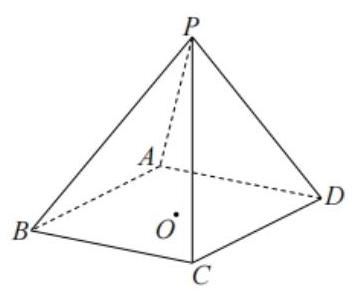
\includegraphics[max width=0.3\textwidth]{images/bo_d5jm9o77aajc7383vmi0_74_1097_1124_352_292_0.jpg}
\end{center}
\hspace*{3em} 

(1)设 \({AD} = {3\sqrt{2}},{PA} = 5\) ，将 \(\bigtriangleup  {POA}\) 绕 \({PO}\) 旋转一周,求所得旋转体的体积;

(2)设 \({PA} = {AD},E\) 为棱 \({PD}\) 中点，求直线 \({BD}\) 与平面 \({AEC}\) 所成角的大小.

【解析】(1) 所得旋转体是以 \({OA}\) 为底面半径, \({OP}\) 为高的圆锥,

计算得 \({OA} = 3,{OP} = 4\) ,则所得旋转体的体积 \(V = \frac{1}{3}\pi  \times  {3}^{2} \times  4 \; = {12\pi }\) ;

(2)以 \(O\) 为原点, \({OB}\) 为 \(x\) 轴, \({OC}\) 为 \(y\) 轴, \({OP}\) 为 \(z\) 轴,

建立空间直角坐标系，不妨设 \({OB} = 2\) ，

则 \(B\left( {2,0,0}\right) ,D\left( {-2,0,0}\right) ,A\left( {0, - 2,0}\right) ,C\left( {0,2,0}\right) ,P\left( {0,0,2}\right) ,E\left( {-1,0,1}\right)\) ,

\(\overrightarrow{BD} = \left( {-4,0,0}\right) ,\overrightarrow{AC} = \left( {0,4,0}\right) ,\overrightarrow{AE} = \left( {-1,2,1}\right)\) ,

设平面 \({AEC}\) 的法向量 \(\overrightarrow{n} = \left( {x,y,z}\right)\) ,

则 \(\left\{  \begin{array}{l} \overrightarrow{n} \cdot  \overrightarrow{AC} = {4y} = 0 \\  \overrightarrow{n} \cdot  \overrightarrow{AE} =  - x + {2y} + z = 0 \end{array}\right.\) ,令 \(x = 1\) ,得 \(\overrightarrow{n} = \left( {1,0,1}\right)\) ,

设直线 \({BD}\) 与平面 \({AEC}\) 所成角为 \(\theta\) ,则 \(\sin \theta  = \frac{\left| \overrightarrow{n} \cdot  \overrightarrow{BD}\right| }{\left| \overrightarrow{n}\right| \left| \overrightarrow{BD}\right| } = \frac{1}{\sqrt{2}} = \frac{\sqrt{2}}{2}\) ,

因为 \(\theta  \in  \left\lbrack  {0,\frac{\pi }{2}}\right\rbrack\) ,所以直线 \({BD}\) 与平面 \({AEC}\) 所成角的大小为 \(\frac{\pi }{4}\) .

【例题】3. (2024上海春考)如图，已知 \({PA}\) 、 \({PB}\) 、 \({PC}\) 为圆锥三条母线，且 \({AB} = {AC}\) .

(1)证明: \({PA} \bot  {BC}\) ；

(2)若圆锥侧面积为 \(\sqrt{3}\pi ,{BC}\) 为底面直径， \({BC} = 2\) ，求二面角 \(B - {PA} - C\) 的大小.

\begin{center}
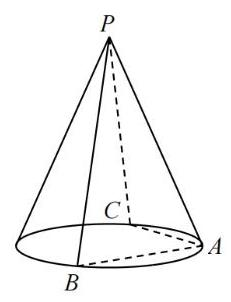
\includegraphics[max width=0.2\textwidth]{images/bo_d5jm9o77aajc7383vmi0_75_1221_241_231_302_0.jpg}
\end{center}
\hspace*{3em} 

【解析】(1) 取 \({BC}\) 中点 \(M\) ,连接 \({PM},{AM}\) ,

因为 \({AB} = {AC}\) ，所以 \({AB} = {AC} \Rightarrow  {AM}\bot {BC}\) ，

因为 \({PB} = {PC}\) ，所以 \({PB} = {PC} \Rightarrow  {PM}\bot {BC}\) ，

因为 \({PM} \subset\) 平面 \({PMC} \subset\) Áæ \({PMA},{AM} \subset\) 平面 \({AMC} \subset\) Áæ \({PMA},{PM} \cap  {AM} \; = M\) ,

所以 \({BC} \bot\) 平面 \({BC} \bot\) ̃aePAM,

因为 \({PA} \subset\) 平面 \({PA} \subset\) 入 \({aePAM}\) ,所以 \({PA} \bot  {BC}\) ;

(2)法一:圆锥侧面积 \(S = {\pi r} \cdot  l = \sqrt{3}\pi\) ，底面半径 \(r = 1\) ，

则母线 \(S = {\pi r} \cdot  l = \sqrt{3}\pi ,r = 1,\therefore l = \sqrt{3}\) ,

取底面中心 \(O\) ,因为 \({PO} \bot\) 平面 \({ABC}\) ,所以 \({ABC},\therefore {PO} = \sqrt{2}\) ,

过点 \(O\) 作 \({OH} \bot  {PA}\) 交 \({PA}\) 于点 \(H\) ，连接 \({BH}\) ，

由 (1) 和三垂线定理得 \({BH} \bot  {AP}\) ,

所以 \(\angle {OHB}\) 即二面角 \(B - {PA} - O\) 的平面角,

由等面积法得 \({OH} = \frac{{OA} \cdot  {OP}}{AP} = \frac{\sqrt{6}}{3}\) ，所以 \(\tan \angle {OHB} = \frac{OB}{OH} = \frac{\sqrt{6}}{2}\) ，

由对称性 \(B - {PA} - C = {2B} - {PA} - O = 2\angle {OHB}\) ,

\begin{center}
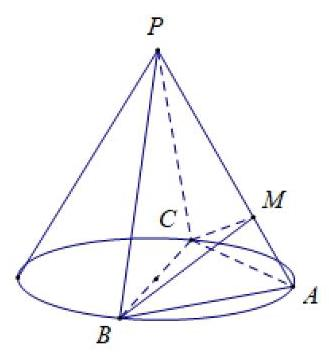
\includegraphics[max width=0.2\textwidth]{images/bo_d5jm9o77aajc7383vmi0_75_1127_946_329_354_0.jpg}
\end{center}
\hspace*{3em} 

\(\tan 2\angle {OHB} = \frac{\sqrt{6}}{1 - \frac{3}{2}} =  - 2\sqrt{6},\)

所以二面角 \(B - {PA} - C\) 大小为 \(\pi  - \arctan 2\sqrt{6}\) .

法二:作 \({BM}\) 垂直于 \({PA}\) ，垂足为 \(M\) ，连接 \({CM}\) ，

由题意得 \(\bigtriangleup  {PAB} \cong   \bigtriangleup  {PAC}\) ，故 \({CM}\bot {PA}\) ，

即 \(\angle {BMC}\) 为所求二面角的平面角,

在 \(\bigtriangleup  {PAB}\) 内，不妨设 \({AB}\) 边上的高为 \(h\) ，故 \(h = \sqrt{{\sqrt{3}}^{2} - {\left( \frac{\sqrt{2}}{2}\right) }^{2}} = \; \frac{\sqrt{10}}{2}\) ,

由 \(\frac{1}{2}h\left| {AB}\right|  = \frac{1}{2}\left| {BM}\right|  \cdot  \left| {PA}\right|\) ,得 \({BM} = {CM} = \frac{\sqrt{15}}{3}\) ,

在 \(\bigtriangleup {BCM}\) 中,由余弦定理得 \(\cos \angle {BMC} = \frac{{\left( \frac{\sqrt{15}}{3}\right) }^{2} + {\left( \frac{\sqrt{15}}{3}\right) }^{2} - {2}^{2}}{2 \times  \frac{\sqrt{15}}{3} \times  \frac{\sqrt{15}}{3}} =  - \frac{1}{5}\) ,

故二面角 \(B - {PA} - C\) 的大小为 \(\pi  - \arccos \frac{1}{5}\) .

法三: 取底面中心 \(O\) ,以 \({OB}\) 为 \(x\) 轴, \({OA}\) 为 \(y\) 轴,

\begin{center}
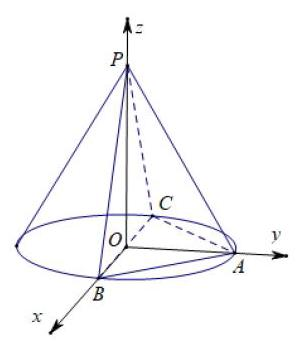
\includegraphics[max width=0.2\textwidth]{images/bo_d5jm9o77aajc7383vmi0_75_1151_1692_296_346_0.jpg}
\end{center}
\hspace*{3em} 

\({OP}\) 为 \(z\) 轴,建立空间直角坐标系,

因为圆锥侧面积为 \(\sqrt{3}\pi ,{BC}\) 为底面直径, \({BC} = 2\) ,

所以底面半径为 1,母线长为 \(\sqrt{3}\) ,所以 \({PO} = \sqrt{P{A}^{2} - A{O}^{2}} = \sqrt{2}\) ,

则 \(P\left( {0,0,\sqrt{2}}\right) ,A\left( {0,1,0}\right) ,B\left( {1,0,C}\right) ,C\left( {-1,0,0}\right)\) ,

故 \(\overrightarrow{PA} = \left( {0,1, - \sqrt{2}}\right) ,\overrightarrow{PB} = \left( {1,0, - \sqrt{2}}\right) ,\overrightarrow{PC} = \left( {-1,0, - \sqrt{2}}\right)\) ,

设 \({\overrightarrow{n}}_{1} = \left( {{x}_{1},{y}_{1},{z}_{1}}\right)\) 为面 \({PAB}\) 的法向量,则

\(\left\{  {\begin{array}{l} \overrightarrow{{n}_{1}} \cdot  \overrightarrow{PA} = 0 \\  \overrightarrow{{n}_{1}} \cdot  \overrightarrow{PB} = 0 \end{array} \Rightarrow  \left\{  {\begin{array}{l} {y}_{1} - \sqrt{2}{z}_{1} = 0 \\  {x}_{1} - \sqrt{2}{z}_{1} = 0 \end{array},}\right. }\right.\)

令 \({x}_{1} = \sqrt{2}\) ,则 \({y}_{1} = \sqrt{2},{z}_{1} = 1\) ,所以 \(\overrightarrow{{n}_{1}} = \left( {\sqrt{2},\sqrt{2},1}\right)\) .

设 \({\overrightarrow{n}}_{2} = \left( {{x}_{2},{y}_{2},{z}_{2}}\right)\) 为面 \({PAC}\) 的法向量,则 \(\left\{  {\begin{array}{l} {\overrightarrow{n}}_{2} \cdot  \overrightarrow{PA} = 0 \\  {\overrightarrow{n}}_{2} \cdot  \overrightarrow{PC} = 0 \end{array} \Rightarrow  \left\{  \begin{array}{l} {y}_{2} - \sqrt{2}{z}_{2} = 0 \\   - {x}_{2} - \sqrt{2}{z}_{2} = 0 \end{array}\right. }\right.\) ,

令 \({x}_{2} =  - \sqrt{2}\) ,则 \({y}_{2} = \sqrt{2},{z}_{2} = 1\) ,所以 \(\overrightarrow{{n}_{2}} = \left( {-\sqrt{2},\sqrt{2},1}\right)\) .

则 \(\cos {\overrightarrow{n}}_{1},{\overrightarrow{n}}_{2} = \frac{{\overrightarrow{n}}_{1} \cdot  {\overrightarrow{n}}_{2}}{\left| {\overrightarrow{n}}_{1}\right| \left| {\overrightarrow{n}}_{2}\right| } = \frac{-2 + 2 + 1}{\sqrt{5} \times  \sqrt{5}} =  - \frac{1}{5}\) ,

所以二面角 \(B - {PA} - C\) 的大小为 \(\pi  - \arccos \frac{1}{5}\) .

\begin{center}
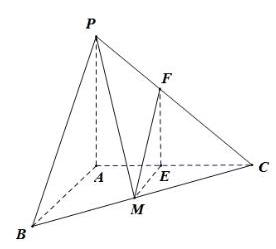
\includegraphics[max width=0.2\textwidth]{images/bo_d5jm9o77aajc7383vmi0_76_1176_590_276_249_0.jpg}
\end{center}
\hspace*{3em} 

【例题】4. (2023 上海春考) 已知三棱锥 \(P - {ABC}\) 中， \({PA}\bot\) 平面 \({ABC},{AB}\bot {AC},{PA} = {AB} = 3,{AC} =\) 4, \(M\) 为 \({BC}\) 中点，过点 \(M\) 分别作平行于平面 \({PAB}\) 的直线交 \({AC}\) 、 \({PC}\) 于点 \(E\) 、 \(F\) .

(1)求直线 \({PM}\) 与平面 \({ABC}\) 所成角的大小；

(2)证明: \({ME}//\) 平面 \({PAB}\) ，并求直线 \({ME}\) 到平面 \({PAB}\) 的距离.

【解析】(1)连接 \({AM},{PM}\) ,

\(\because {PA} \bot\) 平面 \({ABC}\) ,

\(\therefore \angle {PMA}\) 为直线 \({PM}\) 与平面 \({ABC}\) 所成的角，

因为 \({PA} = {AB} = 3,{AC} = 4\) ，所以 \({BC} = 5,{AM} = \frac{5}{2},\)

所以 \({PA} = {AB} = 3,{AC} = 4 \Rightarrow  {BC} = 5,{AM} = \frac{5}{2}\)

\(\Rightarrow  \tan \angle {PMA} = \frac{PA}{AM} = \frac{3}{\frac{5}{2}} = \frac{6}{5}\) ，所以 \(\frac{3}{\frac{5}{2}} = \frac{6}{5} \Rightarrow  \angle {PMA} = \arctan \frac{6}{5}\) ， \(\therefore\) ，

所以直线 \({PM}\) 与平面 \({ABC}\) 所成的角 \(\arctan \frac{6}{5}\) .

(2)因为 \({ME}//\) 平面 \({PAB},{ME} \subset\) 平面 \({ABC}\) ，平面 \({ABC} \cap\) 平面 \({PAB} = {AB}\) ，

所以 \({AB} \Rightarrow  {ME}//{AB}\) ，又 \(M\) 为 \({BC}\) 中点，所以 \(E\) 为 \({AC}\) 中点，

\({AE}\) 即为直线 \({ME}\) 到平面 \({PAB}\) 的距离，所以直线 \({ME}\) 到平面 \({PAB}\) 的距离 \(= 2\) .

【例题】5. (2023上海秋考)如图，在直四棱柱 \({ABCD} - {A}_{1}{B}_{1}{C}_{1}{D}_{1}\) 中，

\begin{center}
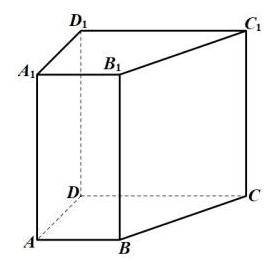
\includegraphics[max width=0.2\textwidth]{images/bo_d5jm9o77aajc7383vmi0_76_1186_1381_270_263_0.jpg}
\end{center}
\hspace*{3em} 

\({AB}//{DC},{AB} \bot  {AD},{AB} = 2,{AD} = 3,{DC} = 4\) .

(1)求证:直线 \({A}_{1}B//\) 平面 \({DC}{C}_{1}{D}_{1}\) ；

(2)若直四棱柱 \({ABCD} - {A}_{1}{B}_{1}{C}_{1}{D}_{1}\) 的体积为36，

求二面角 \({A}_{1} - {BD} - A\) 的大小.

【解析】法一: (几何法)

(1)取 \({DC}\) 中点 \(E\) ，连接 \({DE}\) ， \({AB}//{DC}\) ，即 \({AB}//{DE}\) ，

且 \({AB} = 2,{DC} = 4\) ，所以 \({AB} = {DE}\) ，

所以四边形 \({ABED}\) 为平行四边形,所以 \({AD}//{EB},{AD} = {EB}\) ，

又在直四棱柱 \({ABCD} - {A}_{1}{B}_{1}{C}_{1}{D}_{1}\) 中，所以 \({AD}//{A}_{1}{D}_{1},{AD} = {A}_{1}{D}_{1}\) ，

所以 \({BE} = {A}_{1}{D}_{1}\) 且 \({BE}//{A}_{1}{D}_{1}\) ，所以四边形 \({A}_{1}{BE}{D}_{1}\) 为平行四边形，

所以 \({A}_{1}B//{D}_{1}E\) ,又 \({A}_{1}B \subset\) 平面 \({DC}{C}_{1}D,{D}_{1}E \subset\) 平面 \({DC}{C}_{1}D\) ,

所以 \({A}_{1}B//\) 面 \({DC}{C}_{1}D\) ;

(2) 因为四柱体 \({ABCD} - {A}_{1}{B}_{1}{C}_{1}{D}_{1}\) 的体积为 36,

所以 \({36} = {S}_{ABCD} \cdot  D{D}_{1} = \frac{1}{2}\left( {2 + 4}\right)  \times  3 \cdot  D{D}_{1}\) ,解得 \(D{D}_{1} = 4\) ,

过 \(A\) 作 \({AF} \bot  {BD}\) 于 \(F\) ,连接 \({AF}\) ,则 \(\angle {A}_{1}{FA}\) 为二面角的平面角,

计算得 \({BD} = \sqrt{A{B}^{2} + A{D}^{2}} = \sqrt{13}\) ，则 \({AF} = \frac{{AD} \cdot  {AB}}{BD} = \frac{2 \times  3}{\sqrt{13}}\) ，

则 \(\tan \angle {A}_{1}{FA} = \frac{A{A}_{1}}{AF} = 4 \div  \frac{6}{\sqrt{13}} = \frac{2\sqrt{13}}{3}\) ，

易得二面角 \({A}_{1} - {BD} - A\) 的平面角为锐角，

所以二面角 \({A}_{1} - {BD} - A\) 的大小为 \(\arctan \frac{2\sqrt{13}}{3}\) .

法二:(空间向量)

以 \(D\) 为坐标原点, \(\overrightarrow{DA}\text{ 、 }\overrightarrow{DC}\text{ 、 }\overrightarrow{D{D}_{1}}\) 的方向分别为 \(x,y,z\) 轴的正方向,

建立空间直角坐标系,

(1) \({A}_{1}\left( {3,0,4}\right) ,B\left( {3,2,0}\right) ,D\left( {0,0,0}\right) ,B\left( {3,2,0}\right) ,{A}_{1}\left( {3,0,4}\right)\) ,所以 \(\overrightarrow{{A}_{1}B} = \left( {0,2, - 4}\right)\) .

由 \({AD} \bot\) 面 \({CD}{D}_{1}{C}_{1}\) 得 \(\overrightarrow{DA}\) 是面 \({CD}{D}_{1}{C}_{1}\) 的一个法向量,

\(\overrightarrow{DA} = \left( {3,0,0}\right)\) ,所以 \(\overrightarrow{DA} \cdot  \overrightarrow{{A}_{1}B} = 0\) ,所以 \(\overrightarrow{{A}_{1}B} \bot  \overrightarrow{DA}\) ,

又 \({A}_{1}B \subset\) 平面 \({DC}{C}_{1}D\) ,所以 \(\overrightarrow{DA} \cdot  \overrightarrow{{A}_{1}B} = 0 \Rightarrow  \overrightarrow{{A}_{1}B} \bot  \overrightarrow{DA},\therefore {A}_{1}B//\) 平面 \({DC}{C}_{1}{D}_{1}\) ;

(2) \(D\left( {0,0,0}\right)\) ， \({A}_{1}\left( {3,0,4}\right)\) ， \(B\left( {3,2,0}\right)\) ，所以 \(\overrightarrow{D{A}_{1}} = \left( {3,0,4}\right)\) ， \(\overrightarrow{DB} = \left( {3,2,0}\right)\) ，

其中平面 \({ABD}\) 的一个法向量为 \(\overrightarrow{D{D}_{1}} = \left( {0,0,4}\right)\) ,

设平面 \({A}_{1}{BD}\) 的一个法向量为 \(\overrightarrow{n} = \left( {x,y,z}\right)\) ,则 \(\left\{  \begin{array}{l} \overrightarrow{n} \cdot  \overrightarrow{DA} = {3x} + {4z} = 0 \\  \overrightarrow{n} \cdot  \overrightarrow{DB} = {3x} + {2y} = 0 \end{array}\right.\) ,

取 \(x = 4\) ，则 \(\overrightarrow{n} = \left( {4, - 6, - 3}\right)\) ，设二面角 \({A}_{1} - {BD} - A\) 的大小为 \(\theta\) ，

则 \(\cos \theta  = \left| {\cos \overrightarrow{n},\overrightarrow{D{D}_{1}}}\right|  = \frac{\left| \overrightarrow{n} \cdot  \overrightarrow{D{D}_{1}}\right| }{\left| \overrightarrow{n}\right|  \cdot  \left| \overrightarrow{D{D}_{1}}\right| } = \frac{12}{4\sqrt{{4}^{2} + {6}^{2} + {3}^{2}}} = \frac{3\sqrt{61}}{61}\) ，

易得二面角 \({A}_{1} - {BD} - A\) 的平面角为锐角,

所以 \(\theta  = \arccos \frac{3\sqrt{61}}{61}\) . 2025 版上海高考真题及模拟训练合集(下册)

\section*{2. 模拟练习}

注:用真题简单练习即可, 这个作为大题第一道不会难, 只要牢牢掌握基础

\begin{center}
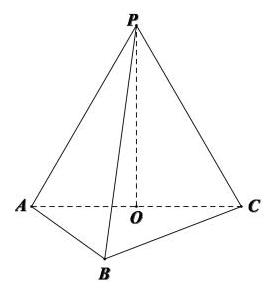
\includegraphics[max width=0.2\textwidth]{images/bo_d5jm9o77aajc7383vmi0_78_1177_374_268_288_0.jpg}
\end{center}
\hspace*{3em} 

【练习】1. (2022 上海秋考) 如图所示三棱锥,底面为等边 \(\bigtriangleup {ABC},O\) 为 \({AC}\) 中点, \({PO} \bot\) 平面 \({ABC},{AP} = {AC} = 2\) .

(1)求三棱锥 \(P - {ABC}\) 的体积;

(2)若 \(M\) 为 \({BC}\) 中点，求 \({PM}\) 与平面 \({PAC}\) 所成角的大小.

【解析】(1) 因为 \({PO} \bot\) 平面 \({ABC},{AP} = {AC} = 2\) ,所以 \({PO} = \sqrt{{2}^{2} - {1}^{2}} = \sqrt{3}\) , 所以三棱锥 \(P - {ABC}\) 的体积 \(V = \frac{1}{3} \cdot  \frac{\sqrt{3}}{4}A{C}^{2} \cdot  {PO} = 1\) ;

(2)法一:取 \({OC}\) 中点 \(N\) ，又 \(M\) 为 \({BC}\) 中点，所以 \({MN}//{OB}\) ，

在等边三角形 \({ABC}\) 中， \({OB}\bot {AC}\) ，

\begin{center}
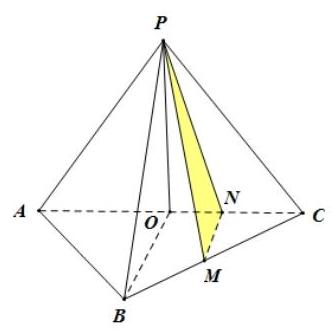
\includegraphics[max width=0.2\textwidth]{images/bo_d5jm9o77aajc7383vmi0_78_1124_702_332_332_0.jpg}
\end{center}
\hspace*{3em} 

又 \({PO} \bot\) 平面 \({ABC},{OB} \subset\) 平面 \({ABC}\) ，所以 \({PO} \bot  {OB}\) ，

因为 \({PO} \cap  {AC} = O\) ，所以 \({OB}\bot\) 平面 \({ABC}\) ，所以 \({MN}\bot\) 平面 \({ABC}\) ，

从而 \({PM}\) 与平面 \({PAC}\) 所成角为 \(\angle {PMN}\) ,

计算得 \({MN} = \frac{1}{2}{OB} = \frac{\sqrt{3}}{2},{PN} = \sqrt{{\left( \sqrt{3}\right) }^{2} + {\left( \frac{1}{2}\right) }^{2}} = \frac{\sqrt{13}}{2}\) ,

所以 \(\tan \angle {PMN} = \frac{MN}{PN} = \frac{\sqrt{3}}{\sqrt{13}} = \frac{\sqrt{39}}{13}\) ，

又 \(\angle {PMN}\) 为锐角，所以 \(\angle {PMN} = \arctan \frac{\sqrt{39}}{13}\) ，

所以 \({PM}\) 与平面 \({PAC}\) 所成角的大小为 \(\arctan \frac{\sqrt{39}}{13}\) .

法二: 以 \(O\) 为原点, \({OB}\) 方向为 \(x\) 轴正半轴, \({OC}\) 方向为 \(y\) 轴正半轴,

\({OP}\) 方向为 \(z\) 轴正半轴建立空间直角坐标系,

易得平面 \({PAC}\) 的法向量为 \(\overrightarrow{n} = \left( {1,0,0}\right)\) ,

又 \(M\) 为 \({BC}\) 中点，所以 \(P\left( {0,0,\sqrt{3}}\right)\) ， \(M\left( {\frac{\sqrt{3}}{2},\frac{1}{2},0}\right)\) ，所以 \(\overrightarrow{PM} = \left( {\frac{\sqrt{3}}{2},\frac{1}{2}, - \sqrt{3}}\right)\) ，

设 \({PM}\) 与平面 \({PAC}\) 所成角为 \(\theta\) ，则 \(\sin \theta  = \frac{\left| \overrightarrow{n} \cdot  \overrightarrow{PM}\right| }{\left| \overrightarrow{n}\right| \left| \overrightarrow{PM}\right| } = \frac{\frac{\sqrt{3}}{2}}{2} = \frac{\sqrt{3}}{4}\) ，

又 \(\theta\) 为锐角，所以 \({PM}\) 与平面 \({PAC}\) 所成角的大小为 \(\arcsin \frac{\sqrt{3}}{4}\) .

\begin{center}
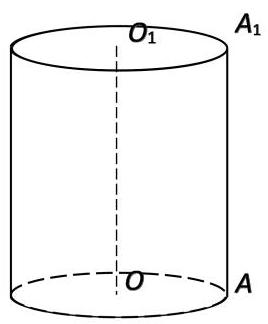
\includegraphics[max width=0.2\textwidth]{images/bo_d5jm9o77aajc7383vmi0_78_1134_1596_268_324_0.jpg}
\end{center}
\hspace*{3em} 

【练习】2. (2022 上海春考) 设有底面半径为 1 的圆柱 \(O{O}_{1},A{A}_{1}\) 为圆柱的母线.

(1)若 \(A{A}_{1} = 4\) ，设 \(M\) 为 \(A{A}_{1}\) 的中点，求直线 \(M{O}_{1}\) 与圆柱上底面所成角;

(2)若过 \(O{O}_{1}\) 的轴截面为正方形，求圆柱 \(O{O}_{1}\) 的侧面积和体积.

【解析】(1) 由圆柱的性质得 \(A{A}_{1} \bot\) 圆柱上底面，连接 \(M{O}_{1}\) ,

则 \(\angle M{O}_{1}{A}_{1}\) 即为直线 \(M{O}_{1}\) 与圆柱上底面所成角,

因为 \(A{A}_{1} = 4\) ,设 \(M\) 为 \(A{A}_{1}\) 的中点,所以 \(M{A}_{1} = 2\) ,

又 \({O}_{1}{A}_{1} = 1\) ,所以 \(\tan \angle M{O}_{1}{A}_{1} = \frac{M{A}_{1}}{{O}_{1}{A}_{1}} = 2\) ,

故直线 \(M{O}_{1}\) 与圆柱上底面所成角为 \(\arctan 2\) ;

(2)若过 \(O{O}_{1}\) 的轴截面为正方形，则母线 \(A{A}_{1} = 2\) ，

所以圆柱 \(O{O}_{1}\) 的侧面积为 \({2\pi rh} = {4\pi }\) ,体积为 \(\pi {r}^{2}h = {2\pi }\) .

\begin{center}
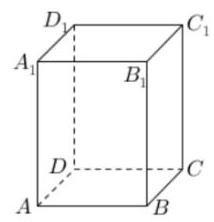
\includegraphics[max width=0.2\textwidth]{images/bo_d5jm9o77aajc7383vmi0_79_1228_331_214_222_0.jpg}
\end{center}
\hspace*{3em} 

【练习】3. (2021 上海秋考) 如图,在长方体 \({ABCD} - {A}_{1}{B}_{1}{C}_{1}{D}_{1}\) 中,已知 \({AB} = {BC} =\) 2, \(A{A}_{1} = 3\) .

(1)若 \(P\) 是棱 \({A}_{1}{D}_{1}\) 上的动点,求三棱锥 \(C - {PAD}\) 的体积;

(2)求直线 \(A{B}_{1}\) 与平面 \({AC}{C}_{1}{A}_{1}\) 的夹角大小.

【解析】(1) 如图,在长方体 \({ABCD} - {A}_{1}{B}_{1}{C}_{1}{D}_{1}\) 中,

\({V}_{C - {PAD}} = \frac{1}{3}{S}_{\Delta PAD} \cdot  {h}_{C - \text{ 平面 }{PAD}} = \frac{1}{3} \times  \left( {\frac{1}{2} \times  2 \times  3}\right)  \times  2 = 2\) ;

(2) 连接 \({A}_{1}{C}_{1} \cap  {B}_{1}{D}_{1} = O\) ,

\begin{center}
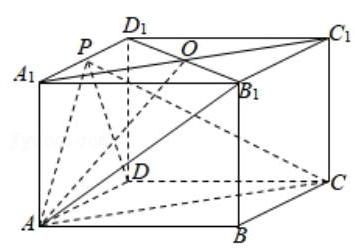
\includegraphics[max width=0.3\textwidth]{images/bo_d5jm9o77aajc7383vmi0_79_1097_640_355_248_0.jpg}
\end{center}
\hspace*{3em} 

因为 \({AB} = {BC}\) ，所以四边形 \({A}_{1}{B}_{1}{C}_{1}{D}_{1}\) 为正方形，则 \(O{B}_{1}\bot O{A}_{1}\) ，

又 \(A{A}_{1} \bot  O{B}_{1},O{A}_{1} \cap  A{A}_{1} = {A}_{1}\) ,所以 \(O{B}_{1} \bot\) 平面 \({AC}{C}_{1}{A}_{1}\) ,

所以直线 \(A{B}_{1}\) 与平面 \({AC}{C}_{1}{A}_{1}\) 所成的角为 \(\angle {OA}{B}_{1}\) ,

所以 \(\sin \angle {OA}{B}_{1} = \frac{O{B}_{1}}{A{B}_{1}} = \frac{\frac{\sqrt{{2}^{2} + {2}^{2}}}{2}}{\sqrt{{2}^{2} + {3}^{2}}} = \frac{\sqrt{26}}{13}\) .

所以直线 \(A{B}_{1}\) 与平面 \({AC}{C}_{1}{A}_{1}\) 所成的角为 \(\arcsin \frac{\sqrt{26}}{13}\) .

【练习】4. (2021 上海春考) 四棱锥 \(P - {ABCD}\) ，底面为正方形 \({ABCD}\) ，边长为4， \(E\) 为 \({AB}\) 中点， \({PE}\bot\) 平面 \({ABCD}\) .

\begin{center}
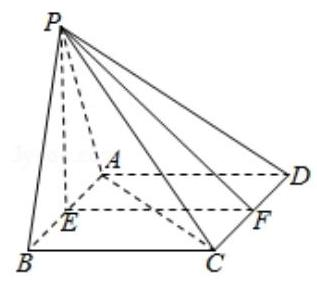
\includegraphics[max width=0.2\textwidth]{images/bo_d5jm9o77aajc7383vmi0_79_1135_1028_317_281_0.jpg}
\end{center}
\hspace*{3em} 

(1)若 \(\bigtriangleup  {PAB}\) 为等边三角形，求四棱锥 \(P - {ABCD}\) 的体积；

(2)若 \({CD}\) 的中点为 \(F\) ， \({PF}\) 与平面 \({ABCD}\) 所成角为 \({45}^{ \circ  }\) ，求 \({PC}\) 与 \({AD}\) 所成角的大小.

【解析】(1)因为 \({\Delta PAB}\) 为等边三角形,且 \(E\) 为 \({AB}\) 中点, \({AB} = 4\) ,所以 \({PE} = \; 2\sqrt{3}\) ,

又 \({PE} \bot\) 平面 \({ABCD}\) ,

所以四棱锥 \(P - {ABCD}\) 的体积 \(V = \frac{1}{3}{PE} \cdot  {S}_{\text{ 正方形 }{ABCD}} = \frac{1}{3} \times  2\sqrt{3 \cdot  4} = \frac{{32}\sqrt{3}}{3}\) .

(2)因为 \({PE} \bot\) 平面 \({ABCD}\) ，

所以 \(\angle {PFE}\) 为 \({PF}\) 与平面 \({ABCD}\) 所成角为 \({45}^{ \circ  }\) ,即 \(\angle {PFE} = {45}^{ \circ  }\) ,

所以 \({\Delta PEF}\) 为等腰直角三角形,

因为 \(E,F\) 分别为 \({AB},{CD}\) 的中点,所以 \({PE} = {FE} = 4\) ,

所以 \({PB} = \sqrt{P{E}^{2} + B{E}^{2}} = {2\sqrt{5}}\) ，

因为 \({AD}//{BC}\) ，所以 \(\angle {PCB}\) 或其补角即为 \({PC}\) 与 \({AD}\) 所成角，

因为 \({PE} \bot\) 平面 \({ABCD}\) ,所以 \({PE} \bot  {BC}\) ,

又 \({BC} \bot  {AB},{PE} \cap  {AB} = E,{PE}\text{ 、 }{AB} \subset\) 平面 \({PAB}\) ,

所以 \({BC} \bot\) 平面 \({PAB}\) ,所以 \({BC} \bot  {PB}\) ,

在 Rt \({\Delta PBC}\) 中, \(\tan \angle {PCB} = \frac{PB}{BC} = \frac{2\sqrt{5}}{4} = \frac{\sqrt{5}}{2}\) ,

故 \({PC}\) 与 \({AD}\) 所成角的大小为 \(\arctan \frac{\sqrt{5}}{2}\) .

【练习】5. (2020 上海春考) 已知四棱锥 \(P - {ABCD}\) ，底面 \({ABCD}\) 为正方形，边长为3， \({PD} \bot\) 平面 \({ABCD}\) .

(1)若 \({PC} = 5\) ，求四棱锥 \(P - {ABCD}\) 的体积;

\begin{center}
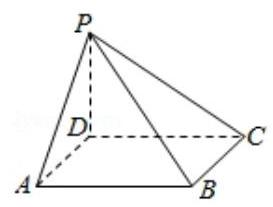
\includegraphics[max width=0.2\textwidth]{images/bo_d5jm9o77aajc7383vmi0_80_1176_234_273_207_0.jpg}
\end{center}
\hspace*{3em} 

(2)若直线 \({AD}\) 与 \({BP}\) 的夹角为 \({60}^{ \circ  }\) ，求 \({PD}\) 的长.

【解析】(1) 因为 \({PD} \bot\) 平面 \({ABCD}\) ,所以 \({PD} \bot  {DC}\) .

因为 \({CD} = 3\) ,所以 \({PC} = 5\) ,所以 \({PD} = 4\) ,

所以 \({V}_{P - {ABCD}} = \frac{1}{3} \times  {3}^{2} \times  4 = {12}\) ,所以四棱锥 \(P - {ABCD}\) 的体积为 12 .

(2)因为四边形 \({ABCD}\) 是正方形， \({PD} \bot\) 平面 \({ABCD}\) ，

所以 \({BC} \bot  {PD},{BC} \bot  {CD}\) ,又因为 \({PD} \cap  {CD} = D\) ,

所以 \({BC} \bot\) 平面 \({PCD}\) ,所以 \({BC} \bot  {PC}\) ,

因为异面直线 \({AD}\) 与 \({PB}\) 所成角为 \({60}^{ \circ  },{BC}//{AD}\) ,

在 Rt \({\Delta PBC}\) 中, \(\angle {PBC} = {60}^{ \circ  },{BC} = 3\) ,故 \({PC} = 3\sqrt{3}\) ,

在 Rt \({\Delta PDC}\) 中, \({CD} = 3\) ,所以 \({PD} = 3\sqrt{2}\) .

\begin{center}
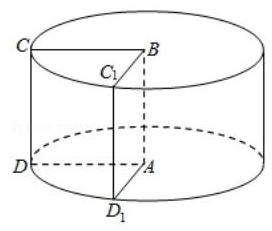
\includegraphics[max width=0.2\textwidth]{images/bo_d5jm9o77aajc7383vmi0_80_1182_764_272_231_0.jpg}
\end{center}
\hspace*{3em} 

【练习】6. (2020 上海秋考) 已知 \({ABCD}\) 是边长为 1 的正方形，正方形 \({ABCD}\) 绕 \({AB}\) 旋转形成一个圆柱.

(1)求该圆柱的表面积；

(2)正方形 \({ABCD}\) 绕 \({AB}\) 逆时针旋转 \(\frac{\pi }{2}\) 至 \({AB}{C}_{1}{D}_{1}\) ，求线段 \(C{D}_{1}\) 与平面 \({ABCD}\) 所成的角.

【解析】(1) 该圆柱的表面由上下两个半径为 1 的圆面

和一个长为 \({2\pi }\) 、宽为 1 的矩形组成,

所以 \(S = 2 \times  \pi  \times  {1}^{2} + {2\pi } \times  1 = {4\pi }\) .

故该圆柱的表面积为 \({4\pi }\) .

(2)因为正方形 \({AB}{C}_{1}{D}_{1}\) ，所以 \(A{D}_{1} \bot  {AB}\) ，

又 \(\angle {DA}{D}_{1} = \frac{\pi }{2}\) ,所以 \(A{D}_{1} \bot  {AD}\) ,

因为 \({AD} \cap  {AB} = A\) ,且 \({AD}\text{ 、 }{AB} \subset\) 平面 \({ADB}\) ,

所以 \(A{D}_{1} \bot\) 平面 \({ADB}\) ,即 \({D}_{1}\) 在面 \({ADB}\) 上的投影为 \(A\) ,

连接 \(C{D}_{1}\) ,则 \(\angle {D}_{1}{CA}\) 即为线段 \(C{D}_{1}\) 与平面 \({ABCD}\) 所成的角,

而 \(\cos \angle {D}_{1}{CA} = \frac{AC}{C{D}_{1}} = \frac{\sqrt{2}}{\sqrt{3}} = \frac{\sqrt{6}}{3}\) ,

所以线段 \(C{D}_{1}\) 与平面 \({ABCD}\) 所成的角为 \(\arccos \frac{\sqrt{6}}{3}\) .

\section*{CD八、排列组合与二项式定理}

注:排列组合基本上都是第 8-9 附近, 难度不大, 考试时有效率的枚举其实就能突破

二项式定理就主要把展开公式, 求各种系数和的方法掌握即可

\section*{板块一:基础客观题}

\section*{1. 真题回顾}

A、二项式定理

【例题】1. (2023 上海春考) 设 \({\left( 1 - 2x\right) }^{4} = {a}_{0} + {a}_{1}x + {a}_{2}{x}^{2} + {a}_{3}{x}^{3} + {a}_{4}{x}^{4}\) ,则 \({a}_{0} + {a}_{4} =\) \_\_\_\_\_.

【答案】 17

【解析】 \({a}_{0} = 1,{a}_{4} = {\left( -2\right) }^{4} = {16},{a}_{0} + {a}_{4} = {17}\) .

【例题】2. (2021 上海春考) 已知 \({\left( 1 + x\right) }^{n}\) 的展开式中,唯有 \({x}^{3}\) 的系数最大,则 \({\left( 1 + x\right) }^{n}\) 的系数和为\_\_\_\_\_.

【答案】64

【解析】由题意得 \({C}_{n}^{3} > {C}_{n}^{2}\) ,且 \({C}_{n}^{3} > {C}_{n}^{4}\) ,所以 \(n = 6\) ,

所以令 \(x = 1\) ,得 \({\left( 1 + x\right) }^{6}\) 的系数和为 \({2}^{6} = {64}\) .

【例题】3. (2017 上海春考) 若 \({\left( x + \frac{2}{x}\right) }^{n}\) 的二项展开式的各项系数之和为 729,则该展开式中常数项的值为\_\_\_\_\_.

【答案】160

【解析】令 \(x = 1\) ,由题意得 \({3}^{n} = {729}\) ,解得 \(n = 6\) .

所以展开式的通项公式为 \({T}_{r + 1} = {2}^{r}{C}_{6}^{r}{x}^{6 - {2r}}\) ,令 \(6 - {2r} = 0\) ,解得 \(r = 3\) ,

所以其展开式中常数项 \(= 8 \times  {20} = {160}\) .

【例题】4. (2015 上海秋考) 在 \({\left( 1 + x + \frac{1}{{x}^{2015}}\right) }^{10}\) 的展开式中, \({x}^{2}\) 项的系数为\_\_\_\_\_(结果用数值表示).

【答案】 4

【解析】因为 \({\left( 1 + x + \frac{1}{{x}^{2015}}\right) }^{10} = {C}_{10}^{0}{\left( 1 + x\right) }^{10}{\left( \frac{1}{{x}^{2015}}\right) }^{0} + {C}_{10}^{1}{\left( 1 + x\right) }^{9}{\left( \frac{1}{{x}^{2015}}\right) }^{1} + \cdots\) ,

所以仅在第一部分中出现 \({x}^{2}\) 项的系数.

再由 \({T}_{r + 1} = {C}_{10}^{r}{x}^{r}\) ,令 \(r = 2\) ,得 \({x}^{2}\) 项的系数为 \({C}_{10}^{2} = .\) 、

B、排列组合

【例题】1. (2022 上海春考) 设由数字 \(1\text{ 、 }2\text{ 、 }3\text{ 、 }4\) 组成上各个位置上数字不能重复的四位数,则大于 2134 的四位数的个数为\_\_\_\_\_.

【答案】 17

【解析】法一: 若首位为 2,则有 \({P}_{3}^{3} - 1 = 5\) 个,

若首位为 3 或 4,均符合题意,有 \({C}_{2}^{1}{P}_{3}^{3} = {12}\) 个,

故大于 2134 的四位数的个数为 17 个;

法二:不大于 2134 的四位数为首位为 1 的和 2134 本身,

有 \({P}_{4}^{4} - {P}_{3}^{3} - 1 = {17}\) 个.

【例题】2. (2021 上海春考) 某人某天需要运动总时长大于等于 60 分钟，现有五项运动可以选择，如表所示，问有几种运动方式组合\_\_\_\_\_. 2025 版上海高考真题及模拟训练合集(下册)

\begin{center}
\adjustbox{max width=\textwidth}{
\begin{tabular}{|c|c|c|c|c|}
\hline
\(A\) 运动 & \(B\) 运动 & \(C\) 运动 & \(D\) 运动 & \(E\) 运动 \\
\cline{1-5}
7 点-8 点 & 8 点 -9 点 & 9 点 -10 点 & 10 点-11 点 & 11 点 -12 点 \\
\cline{1-5}
30 分钟 & 20 分钟 & 40 分钟 & 30 分钟 & 30 分钟 \\
\cline{1-5}
\hline
\end{tabular}
}
\end{center}

【答案】 23

【解析】由题意得,至少要选 2 种运动,并且选 2 种运动的情况中, \({AB}\text{ 、 }{DB}\text{ 、 }{EB}\) 的组合不符合题意; 所以满足条件的运动组合方式为

\({C}_{5}^{2} + {C}_{5}^{3} + {C}_{5}^{4} + {C}_{5}^{5} - 3 = {10} + {10} + 5 + 1 - 3 = {23}\) (种).

【例题】3. (2020 上海春考) 已知 \(A = \{  - 3, - 2, - 1,0,1,2,3\} ,a\text{ 、 }b \in  A\) ,则 \(\left| a\right|  < \left| b\right|\) 的情况有\_\_\_\_\_ 种.

【答案】 18

【解析】当 \(a =  - 3,0\) 种,当 \(a =  - 2,2\) 种,当 \(a =  - 1,4\) 种;

当 \(a = 0,6\) 种,当 \(a = 1,4\) 种; 当 \(a = 2,2\) 种,当 \(a = 3,0\) 种,

故共有 \(2 + 4 + 6 + 4 + 2 = {18}\) 种.

【例题】4. (2020 上海秋考) 从 6 个人挑选 4 个人去值班, 每人值班一天, 第一天安排 1 个人, 第二天安排 1 个人, 第三天安排 2 个人, 则共有\_\_\_\_\_种安排情况.

【答案】 180

【解析】排法共有 \({C}_{6}^{1}{C}_{5}^{1}{C}_{4}^{2} = {180}\) 种.

【例题】5. (2019 上海春考) 首届中国国际进口博览会在上海举行，某高校拟派 4 人参加连续 5 天的志愿者活动，其中甲连续参加 2 天，其他人各参加 1 天，则不同的安排方法有\_\_\_\_\_种(结果用数值表示)

【答案】 24

【解析】在五天里,连续的 2 天,一共有 4 种,剩下的 3 人排列,故有 \(4{P}_{3}^{3} = {24}\) 种. 2025 版上海高考真题及模拟训练合集(下册)

\section*{2. 模拟练习}

【练习】1. (2022 长宁二模) 将编号为 1,2,3,4 的 4 个小球放入 3 个不同的盒子中，每个盒子不空，若放在同一盒子里的 2 个小球编号不相邻，则共有\_\_\_\_\_种不同的放法.

【答案】 18

【解析】先将 2 个小球放在同一盒子里, 要求 2 个小球编号不相邻, 则这 2 个小球编号可为 1 和 3 或 1 和 4 或 2 和 4，共三种情况，再将另外两个小球放到另外 2 个盒子中，则共有 \(3{P}_{3}^{3} = {18}\) 种不同的放法.

【练习】2. (2022 宝山二模) 北京冬奥会从树人中学挑选 3 名志愿者完成 4 项工作，每人至少完成 1 项， 每项工作由 1 人完成，则不同的安排方式共有\_\_\_\_\_.

【答案】36 种

【解析】 \({C}_{4}^{2} \cdot  {P}_{3}^{3} = {36}\)

【练习】3. (2023 金山一模) 从 7 个人中选 4 人负责元旦三天假期的值班工作，其中第一天安排 2 人，第二天和第三天均安排 1 人，且人员不重复，则一共有\_\_\_\_\_种安排方式(结果用数值表示).

【答案】420

【解析】一共有 \({C}_{7}^{2}{C}_{5}^{1}{C}_{4}^{1} = {420}\) 种安排方式.

【练习】4. (2022 黄浦二模) 已知 \(a > 0\) ,若 \({\left( \frac{a}{x} + \frac{x}{2}\right) }^{9}\) 展开式中 \({x}^{5}\) 的系数为 \(\frac{9}{2}\) ,则常数 \(a\) 的值为\_\_\_\_\_.

【答案】 4

【解析】由已知得,通项公式为: \({T}_{r + 1} = {C}_{9}^{r}{\left( \frac{a}{x}\right) }^{9 - r}{\left( \frac{x}{2}\right) }^{r} = {C}_{9}^{r}{a}^{9 - r}{\left( \frac{1}{2}\right) }^{r}{x}^{{2r} - 9}\) 令 \({2r} - 9 = 5\) ,得 \(r = 7\) ,所以 \({x}^{5}\) 的系数为 \({C}_{9}^{7}{a}^{2}{\left( \frac{1}{2}\right) }^{7} = \frac{9}{2}\) ,即 \(a = 4\) .

【练习】5. 已知 \({\left( \sqrt{x} + \frac{1}{2\sqrt[4]{x}}\right) }^{n}\) 的二项展开式中,前三项系数成等差数列,则 \(n =\) (   ).

A. 7 B. 8 C. 9 D. 10.

【答案】 \(B\)

【解析】展开式的通项为 \({T}_{r + 1} = {C}_{n}^{r}{\left( \sqrt{x}\right) }^{n - r} \cdot  {\left( \frac{1}{2\sqrt[4]{x}}\right) }^{r} = {C}_{n}^{r} \cdot  {\left( \frac{1}{2}\right) }^{r}{x}^{\frac{{2n} - {3r}}{4}}\) , 因为前三项系数成等差数列,所以 \({C}_{n}^{0} + {C}_{n}^{2} \cdot  {\left( \frac{1}{2}\right) }^{2} = 2{C}_{n}^{1} \cdot  {\left( \frac{1}{2}\right) }^{1}\) , 即 \({n}^{2} - {9n} + 8 = 0\) ,解得 \(n = 8\) 或 \(n = 1\) (舍去),故选 \(B\) .

【练习】6. 设 \(x \in  R\) 且 \(x \neq  0\) ，则 \(\left( {x + 2}\right) {\left( \frac{1}{x} - 1\right) }^{5}\) 的展开式中常数项为\_\_\_\_\_.

【答案】 3

【解析】因为 \(\left( {x + 2}\right) {\left( \frac{1}{x} - 1\right) }^{5} = x \cdot  {\left( \frac{1}{x} - 1\right) }^{5} + 2 \cdot  {\left( \frac{1}{x} - 1\right) }^{5}\) ,

\({\left( \frac{1}{x} - 1\right) }^{5}\) 的展开式的通项为 \({T}_{r + 1} = {C}_{5}^{r}{\left( \frac{1}{x}\right) }^{5 - r}{\left( -1\right) }^{r} = {\left( -1\right) }^{r}{C}_{5}^{r} \cdot  {x}^{r - 5}\) ,

故展开式中常数项为 \(x \cdot  {\left( -1\right) }^{4} \cdot  {C}_{5}^{4} \cdot  {x}^{-1} + 2 \cdot  {\left( -1\right) }^{5} \cdot  {C}_{5}^{5} = 3\) .

【练习】7. (23 嘉定二模) 已知 \(n \in  N\) ,若 \({C}_{6}^{n} = {P}_{5}^{2}\) ,则 \(n =\) \_\_\_\_\_.

【答案】 3

【解析】因为 \({C}_{6}^{n} = {P}_{5}^{2} = {20} = {C}_{6}^{3}\) ,所以 \(n = 3\) .

【练习】8. (23 徐汇区二模) 若 \(\left( {1 + x}\right) {\left( 1 - 2x\right) }^{2023} = {a}_{0} + {a}_{1}x + {a}_{2}{x}^{2} + \cdots  + {a}_{2024}{x}^{2024},{a}_{i} \in  R(\mathrm{i} = 0,1,2,\cdots\) , 2024),则 \({a}_{1} + {a}_{2} + \cdots  + {a}_{2024} =\) \_\_\_\_\_.

【答案】-3

【解析】令 \(x = 1\) ,得 \({a}_{0} + {a}_{1} + {a}_{2} + \cdots  + {a}_{2024} =  - 2\) ,令 \(x = 0\) ,得 \({a}_{0} = 1\) ,

所以 \({a}_{1} + {a}_{2} + \cdots  + {a}_{2024} =  - 3\) .

2025 版上海高考真题及模拟训练合集(下册)

\section*{板块二: 中档客观题}

\section*{1. 真题回顾}

【例题】1. (2024 上海秋考) 某集合中的元素为不重复的数字组成的三位正整数，若该集合中任意两个数的积均为偶数，则该集合中元素数量的最大值为\_\_\_\_\_.

【答案】329

【解析】该集合中至多只能有 1 个奇数，因此先考虑偶数的情况，再加上单独的奇数即可，

0\textasciitilde 9 中，有 5 个奇数，5 个偶数，需要对 0 进行讨论，

若三位数中，都是偶数，个位是 0 的有 \({P}_{9}^{2} = {72}\) 个，

个位不是 0 的有 \({C}_{4}^{1}{C}_{8}^{1}{C}_{8}^{1} = {256}\) 个,

则该集合中元素数量的最大值为 \({72} + {256} + 1 = {329}\) .

【例题】2. (2023 上海秋考) 已知 \({\left( 1 + {2023}x\right) }^{100} + {\left( {2023} - x\right) }^{100} = {a}_{0} + {a}_{1}x + {a}_{2}{x}^{2} + \cdots  + {a}_{100}{x}^{100}\) ,若 \(k \in  \{ 0\) ，1，2 ...，100)，则使得 \({a}_{k} < 0\) 成立的 \(k\) 的最大值为\_\_\_\_\_.

【答案】 49

【解析】展开式的通项为 \({T}_{r + 1} = {C}_{100}^{r} \cdot  {\left( {2023}x\right) }^{r} + {C}_{100}^{r} \cdot  {2023}^{{100} - r} \cdot  {\left( -x\right) }^{r}\)

\(= {C}_{100}^{r}\left\lbrack  {{2023}^{r} + {\left( -{2023}\right) }^{{100} - r}}\right\rbrack   \cdot  {x}^{r}\) ,所以 \({a}_{k} = {C}_{100}^{k}\left\lbrack  {{2023}^{k} + {\left( -{2023}\right) }^{{100} - k}}\right\rbrack   < 0\) ,

所以 \({2023}^{k} + {\left( -{2023}\right) }^{{100} - k} < 0\) ,显然 \(k\) 为奇数,所以 \({2023}^{k} < {2023}{)}^{{100} - k}\) ,

所以 \(k < {100} - k\) ,所以 \(k < {50}\) ,则使得 \({a}_{k} < 0\) 成立的 \(k\) 的最大值为 49 .

【例题】3. (2013 上海春考) 36 的所有正约数之和可按如下方法得到:因为 \({36} = {2}^{2} \times  {3}^{2}\) ，所以 36 的所有正约数之和为 \(\left( {1 + 3 + {3}^{2}}\right)  + \left( {2 + 2 \times  3 + 2 \times  {3}^{2}}\right)  + \left( {{2}^{2} + {2}^{2} \times  3 + {2}^{2} \times  {3}^{2}}\right)  = \left( {1 + 2 + {2}^{2}}\right) (1 + 3 \; + {3}^{2}) = {91}\) ，参照上述方法，可求得 2000 的所有正约数之和为\_\_\_\_\_.

【答案】 4836

【解析】类比 36 的所有正约数之和的方法,

2000 的所有正约数之和可按如下方法得到: 因为 \({2000} = {2}^{4} \times  {5}^{3}\) ,

所以 2000 的所有正约数之和为 \(\left( {1 + 2 + {2}^{2} + {2}^{3} + {2}^{4}}\right) \left( {1 + 5 + {5}^{2} + {5}^{3}}\right)  = {4836}\) .

可求得 2000 的所有正约数之和为 4836 . 2025 版上海高考真题及模拟训练合集(下册)

\section*{2. 模拟练习}

【练习】1. (2024 届华二) 已知 \({\left( 1 + 2x\right) }^{2023} + {\left( 2 - x\right) }^{2023} = {a}_{0} + {a}_{1}x + {a}_{2}{x}^{2} + \cdots  + {a}_{2022}{x}^{2022} + {a}_{2023}{x}^{2023}\) ,则 \({a}_{0}\) , \({a}_{1},{a}_{2},\cdots ,{a}_{2022},{a}_{2023}\) 中正数的个数为\_\_\_\_\_.

【答案】 1518

【解析】 \({a}_{n} = {C}_{2023}^{n} \times  \left( {{2}^{n} + {\left( -1\right) }^{n}{2}^{{2023} - n}}\right)\) ,当 \({a}_{n} > 0\) 时,

 \circled{1}  \(n\) 为偶数，共 \(\frac{2024}{2} = {1012}\) 项；

 \circled{2}  \(n\) 为奇数且 \({2}^{n} > {2}^{{2023} - n}\) ，则 2023 \(\geq  n > \frac{2023}{2}\) 且 \(n\) 为奇数，共 506 项；故共有 1012+506 = 1518 个.

【练习】2. 若 \({\left( 2x - 1\right) }^{2024} = {a}_{0} + {a}_{1}x + {a}_{2}{x}^{2} + \cdots  + {a}_{2024}{x}^{2024}\left( {x \in  R}\right)\) ，则

\(\frac{1}{2} + \frac{{a}_{2}}{{2}^{2}{a}_{1}} + \frac{{a}_{3}}{{2}^{3}{a}_{1}} + \cdots  + \frac{{a}_{2024}}{{2}^{2024}{a}_{1}} =\_\_\_\_\_.\)

【答案】-1

【解析】 \({\left( 2x - 1\right) }^{2024}\) 的展开式 \({T}_{r + 1} = {C}_{2024}^{r} \cdot  {2}^{{2024} - r} \cdot  {\left( -1\right) }^{r} \cdot  {x}^{{2024} - r}\) ,

当 \(r = {2023}\) 时, \({a}_{1} =  - {2024} \times  2 =  - {4048}\) ; 当 \(x = 0\) 时, \({a}_{0} = 1\) ,

令 \(x = \frac{1}{2}\) 时, \(1 + \frac{1}{2}{a}_{1} + \frac{{a}_{2}}{{2}^{2}} + \frac{{a}_{3}}{{2}^{3}} + \cdots  + \frac{{a}_{2024}}{{2}^{2024}} = 0\) ,

所以 \(\frac{1}{2}{a}_{1} + \frac{{a}_{2}}{{2}^{2}} + \frac{{a}_{3}}{{2}^{3}} + \cdots  + \frac{{a}_{2024}}{{2}^{2024}} =  - 1\) ,

故 \(\frac{1}{2} + \frac{{a}_{2}}{{2}^{2}{a}_{1}} + \frac{{a}_{3}}{{2}^{3}{a}_{1}} + \cdots  + \frac{{a}_{2024}}{{2}^{2024}{a}_{1}} =  - \frac{1}{{a}_{1}} = \frac{1}{4048}\) .

【练习】3. 设 \(a \in  Z\) ，且 \(0 \leq  a < {13}\) ，若 \({51}^{2024} + a\) 能被 13 整除，则 \(a =\) \_\_\_\_\_.

【答案】 1

【解析】 \({51}^{2024} + a = {\left( {52} - 1\right) }^{2024} + a\)

\(= {52}^{2024} - {C}_{2024}^{1} \cdot  {52}^{2023} + {C}_{2024}^{2} \cdot  {52}^{2022} - \cdots  + {C}_{2024}^{2023} \cdot  {52} - {C}_{2023}^{2024} + a\) ,

所以 \({51}^{2024} + a\) 被 13 整除的余数为 \(- 1 + a\) ,而 \(a \in  Z\) ,且 \(0 \leq  a < {13}\) ,

若 \({51}^{2024} + a\) 能被 13 整除,则 \(- 1 + a = 0\) ,得 \(a = 1\) .

【练习】4. 从集合 \(\{ 0,1,2,3,4,5,6,7,8,9\}\) 中任取 3 个不同元素分别作为直线方程 \({Ax} + {By} + C \; = 0\) 中的 \(A\text{ 、 }B\text{ 、 }C\) ，则经过坐标原点的不同直线有\_\_\_\_\_条(用数值表示).

【答案】54

【解析】因为经过坐标原点,所以 \(C = 0\) ,在其他 9 个元素中任选两个为 \(A\text{ 、 }B\) 有 \({P}_{9}^{2}\) 种,

其中 \(\frac{1}{2} = \frac{2}{4} = \frac{3}{6} = \frac{4}{8},\frac{1}{3} = \frac{2}{6} = \frac{3}{9},\frac{1}{4} = \frac{2}{8},\frac{2}{3} = \frac{4}{6} = \frac{6}{9},\frac{3}{4} = \frac{6}{8}\) ,

故重复了 \(\left( {3 + 2 + 1 + 2 + 1}\right)  \times  2 = {18}\) 种 (倒数也是重复的,故要乘 2 ),

所以经过坐标原点的不同直线有 \({P}_{9}^{2} - {18} = {54}\) 条.

【练习】5. 从集合 \(\{ 1,2,3,4,5,6,7,8,9,{10}\}\) 中任取三个不同的元素作为直线 \(l : {ax} + {by} + c = 0\) 中 \(a,b,c\) 的值. 若直线 \(l\) 的倾斜角小于 \({135}^{ \circ  }\) ,且 \(l\) 在 \(x\) 轴上的截距小于 -1,那么不同的直线 \(l\) 有 ( )

A. 109 条 B. 110 条 C. 111 条 D. 120 条

【答案】 \(A\)

【解析】直线 \(l : {ax} + {by} + c = 0\) 可化为 \(y =  - \frac{a}{b}x - \frac{c}{b},l\) 在 \(x\) 轴上的截距为 \(- \frac{c}{a}\)

因为直线 \(l\) 的倾斜角小于 \({135}^{ \circ  }\) ,且 \(l\) 在 \(x\) 轴上的截距小于 -1,

所以 \(- \frac{a}{b} <  - 1, - \frac{c}{a} <  - 1\) ,所以 \(c > a > b\) ,共有 \({C}_{10}^{3} = {120}\) 种,

其中重复的项, \(\left( {c,a,b}\right)\) 从 \(b = 1\) 开始: \(\left( {3,2,1}\right) ,\left( {6,4,2}\right) ,\left( {9,6,3}\right)\) (重复 2 次);

\(\left( {4,2,1}\right) ,\left( {8,4,2}\right)\) (重复 1 次); \(\left( {5,2,1}\right) ,\left( {{10},4,2}\right)\) (重复 1 次);

\(\left( {4,3,1}\right) ,\left( {8,6,2}\right)\) (重复 1 次); \(\left( {5,3,1}\right) ,\left( {{10},6,2}\right)\) (重复 1 次);

\(\left( {5,4,1}\right) ,\left( {{10},8,2}\right)\) (重复 1 次),共 7 个重复组合;

\(b = 2 : \left( {4,3,2}\right) ,\left( {8,6,4}\right)\) (重复 1 次); \(\left( {5,3,2}\right) ,\left( {{10},6,4}\right)\) (重复 1 次);

\(\left( {5,4,2}\right) ,\left( {{10},8,4}\right)\) (重复 1 次)，共 3 个重复组合；

\(b = 3 : \left( {5,4,3}\right) ,\left( {{10},8,6}\right)\) 共 1 个重复组合

所以不同的直线 \(l\) 有 \({120} - 7 - 3 - 1 = {109}\) 条. 故选 \(A\) .

【练习】6. 设非空集合 \(Q \subseteq  M\) ,当 \(Q\) 中所有元素和为偶数时 (集合为单元素时和为元素本身),称 \(Q\) 是 \(M\) 的偶子集. 若集合 \(M = \{ 1,2,3,4,5,6,7\}\) ，则其偶子集 \(Q\) 的个数为\_\_\_\_\_.

【答案】 63

【解析】偶子集可以分为只有奇数、偶数及偶数个奇数和偶数的集合,

奇数有 4 个,偶数有 3 个

只有奇数的有 \({C}_{4}^{2} + 1 = 7\) 个，只有偶数的有 \({C}_{3}^{1} + {C}_{3}^{2} + 1 = 7\) 个，

偶数个奇数和偶数的: 两奇一偶 \({C}_{4}^{2} \cdot  {C}_{3}^{1} = {18}\) 个，两奇二偶 \({C}_{4}^{2} \cdot  {C}_{3}^{2} = {18}\) 个，

两奇三偶 \({C}_{4}^{2} \cdot  {C}_{3}^{3} = 6\) 个,四奇一偶 \({C}_{4}^{4} \cdot  {C}_{3}^{1} = 3\) 个,四奇二偶 \({C}_{4}^{4} \cdot  {C}_{3}^{2} = 3\) 个,

四奇三偶 \({C}_{4}^{4} \cdot  {C}_{3}^{3} = 1\) 个,所以共有 \(7 + 7 + {18} + {18} + 6 + 3 + 3 + 1 = {63}\) 个.

【练习】7. 把 \(1\text{ 、 }2\text{ 、 }3\text{ 、 }4\text{ 、 }5\) 这五个数随机地排成一列组成一个数列,要求该数列恰好先递增后递减,则这样的数列共有\_\_\_\_\_个.

【答案】 14

【解析】从1,2,3,4中选出一个数排在 5 的右侧,其余排在 5 的左侧,

得到先增后减的数列有 \({C}_{4}^{1}\) ,

从1,2,3,4中选出两个数排在 5 的右侧,其余排在 5 的左侧,

得到先增后减的数列有 \({C}_{4}^{2}\) ,

从1,2,3,4中选出三个数排在 5 的右侧,其余排在 5 的左侧,

得到先增后减的数列有 \({C}_{4}^{3}\) ,

故满足条件的数量总个数为 \({C}_{4}^{1} + {C}_{4}^{2} + {C}_{4}^{3} = {14}\) 个.

【练习】8. 某高校派出 2 名女教师、2 名男教师和 1 名学生参加连续五天的志愿者服务工作，每天安排 1 人，每人工作 1 天，如果 2 名男教师不能安排在相邻两天，2 名女教师也是如此，那么符合条件的不同安排方案共有\_\_\_\_\_种。

【答案】 48

【解析】法一: \({P}_{5}^{5} - 2{P}_{2}^{2}{P}_{4}^{4} + {P}_{2}^{2}{P}_{2}^{2}{P}_{3}^{3} = {48}\) (总的排列减去男老师相邻和女老师相邻,

加上男女老师共同相邻).

法二: \({P}_{3}^{3}{P}_{4}^{2} - {P}_{2}^{2}{P}_{2}^{2}{P}_{3}^{2} = {48}\) (男教师不相邻的情况下减去此时女教师相邻的情况).

2025 版上海高考真题及模拟训练合集(下册)

\section*{板块三:压轴客观题}

注:高考还没考察过, 简单练几道难度适合, 思想方法契合高考的即可

\section*{1. 模拟练习}

【练习】1. (2024 届上中)已知 \(A,B,C,D,E,F\) 六个字母以随机顺序排成一行，若小明每次操作可以互换 2 个字母的位置，则小明必须进行 5 次操作才能将六个字母排成 ABCDEF 的顺序的排列情况有\_\_\_\_\_种。

【答案】 120

【解析】考虑模型: 6 个编号 \({ABCDEF}\) 的盒子,6 个编号 \({abcdef}\) 的小球.

首先证明,任意一种放法,最多只需 5 次操作即可让小球与盒子编号对应。

第一次把 \(a\) 与 \(A\) 中的球交换, \(a\) 归位;

第二次把 \(b\) 与 \(B\) 中的球交换, \(b\) 归位;

第三次把 \(c\) 与 \(C\) 中的球交换, \(c\) 归位;

第四次把 \(d\) 与 \(D\) 中的球交换, \(d\) 归位;

第五次把 \(\mathrm{e}\) 与 \(E\) 中的球交换,则 \(\mathrm{e},f\) 同时归位;

其次，我们说明，

若 \(A\) 盒中，放了 \(a\) 球，则剩余五个盒子五个球，最多只需 4 次交换，即可归位；

若 \({AB}\) 盒中，放了 \({ab}\) 球，则他们最多需要 1 次交换，会剩余四个盒子四个求，最多只需 3 次交换， 总共只需 4 次交换即可归位。

若 \({ABC} =\) 个盒子中，放的是 \({abc} =\) 个小球,则此时只需 2 次交换，即可归位；剩余 \({DEF}\) 盒子也只需要操作 2 次，总共只需操作 4 次，不合题意。

故我们可以总结,任意 \(n\left( {n < 6}\right)\) 个盒子中放的小球必有一个不属于这些盒子的小球，否则，将不需要 5 次操作。

以下, \(A\) 盒可以选择 \(\left( {b,c,d,\mathrm{e},f}\right) 5\) 种, \(B\) 盒可以选择 \(\left( {c,d,\mathrm{e},f}\right) 3\) 种, \(C\) 盒可以选择

\(\left( {d,\mathrm{e},f}\right) 3\) 种, \(D\) 盒可选 \(\left( {\mathrm{e},f}\right) 2\) 种, \(E\) 只能放 \(f,F\) 只能放 \(a\) ,共有 \(5 \times  4 \times  3 \times  2 \times  1 = {120}\) 种.

【练习】2. 设项数为 \(m\) 的数列 \(\left\{  {a}_{n}\right\}\) 满足:

 \circled{1}  \({a}_{i} \in  \{  - 1,0,1\} ,\mathrm{i} = 1,2,3,\cdots ,m\) ;

 \circled{2}  对任意 \(1 \leq  k < l \leq  m,k \in  N,l \in  N\) ，都有 \(\left| {{a}_{k} + {a}_{k + 1} + \cdots  + {a}_{l}}\right|  \leq  1\) ，

则这样的数列 \(\left\{  {a}_{n}\right\}\) 共有\_\_\_\_\_个.

【答案】 \({2}^{m + 1} - 1\)

【解析】显然 \(\left\{  {a}_{n}\right\}\) 中取 0 的项不会影响性质 \circled{2} :

把所有取 0 的项去掉,那么剩余的项必须呈 \(- 1,1, - 1,1\cdots\) 或者反过来,不然就会存在相邻和的绝对值大于等于 2,共两种形态,

所以这样的数列 \(\left\{  {a}_{n}\right\}\) 共有 \({C}_{m}^{m} + \left( {{C}_{m}^{m - 1} + {C}_{m}^{m - 2} + \cdots  + {C}_{m}^{0}}\right)  \cdot  2 = {2}^{m + 1} - 1\) 个,其中 \({C}_{m}^{k}\) 指的是数列的 \(m\) 项里面有 \(k\) 个取 0

【练习】3. 已知非空集合 \(A\text{ 、 }B\) 满足以下两个条件:

(i) \(A \cup  B = \{ 1,2,3,4,5,6\} ,A \cap  B = \varnothing\) ;

(ii) \(A\) 的元素个数不是 \(A\) 中的元素, \(B\) 的元素个数不是 \(B\) 中的元素,则有序集合对 \(\left( {A,B}\right)\) 的个数为\_\_\_\_\_.

【答案】 10

【解析】若集合 \(A\) 中只有 1 个元素,则集合 \(B\) 中只有 5 个元素,则 \(1 \notin  A,5 \notin  B\) ,

即 \(5 \in  A,1 \in  B\) ,此时 \(\left( {A,B}\right)\) 有 1 个;

若集合 \(A\) 中只有 2 个元素，则集合 \(B\) 中只有 4 个元素，则 \(2 \notin  A\) ， \(4 \notin  B\) ，

即 \(4 \in  A,2 \in  B\) ，此时有 \({C}_{5}^{2} = 4\) ；

若集合 \(A\) 中只有 3 个元素，则集合 \(B\) 中只有 3 个元素，则 \(3 \notin  A,3 \notin  B\) ， 不满足题意，

若集合 \(A\) 中只有 4 个元素,则集合 \(B\) 中只有 2 个元素,则 \(4 \notin  A,2 \notin  B\) ,

即 \(2 \in  A,4 \in  B\) ,此时有 \({C}_{4}^{3} = 4\) ;

若集合 \(A\) 中只有 5 个元素,则集合 \(B\) 中只有 1 个元素,则 \(5 \notin  A,1 \notin  B\) ,

即 \(1 \in  A,5 \in  B\) ,此时有 \({C}_{4}^{4} = 1\) ,

故有序集合对 \(\left( {A,B}\right)\) 的个数是 \(1 + 4 + 4 + 1 = {10}\) .

【练习】4. (2025 届复附) 一个项数为 6 的正整数数列 \(\left\{  {a}_{n}\right\}\) 满足 \({a}_{1} = 3\) ,且 \({a}_{k + 1} \geq  {a}_{k}\left( {1 \leq  k \leq  5,k \in  N}\right)\) ,若 \({a}_{6}\) 为不大于 10 的偶数，则符合条件的数列 \(\left\{  {a}_{n}\right\}\) 共有\_\_\_\_\_个

【答案】 496

【解析】法一: (分类枚举法)

由题意, \({a}_{1} = 3\) ,且 \({a}_{k + 1} \geq  {a}_{k}\left( {1 \leq  k \leq  5,k \in  N}\right)\) ,

当 \({a}_{6} = 4\) 时， \({a}_{1} = 3\) ，则 \({a}_{2},{a}_{3},{a}_{4},{a}_{5}\) 可以取 3 或 4，且逐项不减小，

此时满足条件的数列 \(\left\{  {a}_{n}\right\}\) 的个数有 5 个;

当 \({a}_{6} = 6,{a}_{1} = 3\) ,则 \({a}_{2},{a}_{3},{a}_{4},{a}_{5}\) 可以取 3 或 4 或 5 或 6,且逐项不减小,

此时满足条件的数列 \(\left\{  {a}_{n}\right\}\) 的个数有 \({C}_{4}^{4} + {C}_{4}^{3} \times  3 + {C}_{4}^{2} \times  3 + {C}_{4}^{1} = {35}\) 个;

当 \({a}_{6} = 8,{a}_{1} = 3\) ,则 \({a}_{2},{a}_{3},{a}_{4},{a}_{5}\) 可以取 3 或 4 或 5 或 6 或 7 或 8,且逐项不减小,

此时满足条件的数列 \(\left\{  {a}_{n}\right\}\) 的个数有 \({C}_{6}^{4} + {C}_{6}^{3} \times  3 + {C}_{6}^{2} \times  3 + {C}_{6}^{1} = {126}\) 个;

当 \({a}_{6} = {10},{a}_{1} = 3\) ,则 \({a}_{2},{a}_{3},{a}_{4},{a}_{5}\) 可以取 3 或 4 或 5 或 6 或 7 或 8 或 9 或 10,

且逐项不减小，

此时满足条件的数列 \(\left\{  {a}_{n}\right\}\) 的个数有 \({C}_{8}^{4} + {C}_{8}^{3} \times  3 + {C}_{8}^{2} \times  3 + {C}_{8}^{1} = {330}\) 个;

综上,满足条件的数列 \(\left\{  {a}_{n}\right\}\) 共有 \(5 + {35} + {126} + {330} = {496}\)

法二:(隔板法)

当 \({a}_{6} = 4\) 时， \({a}_{1} = 3\) ，记 \({b}_{k} = {a}_{k + 1} - {a}_{k}\) ，则 \(\mathop{\sum }\limits_{{k = 1}}^{5}{b}_{k} = 1\) ，且 \({b}_{k} \geq  0\left( {1 \leq  k \leq  5,k \in  N}\right)\)

我们可以把这个问题理解为 5 个自然数的和是 1 , 有多少种情况? 那么就利用隔板法, 我们把他看成 5 个人分 1 个球的问题，先问每个人要 1 个小球，因此总共有 6 个小球，分给 5 个人需要插 4 块板,6 个小球有 5 个缝隙可以插板,有 \({C}_{5}^{4} = 5\) 种

当 \({a}_{6} = 4\) 时, \({a}_{1} = 3\) ,记 \({b}_{k} = {a}_{k + 1} - {a}_{k}\) ,则 \(\mathop{\sum }\limits_{{k = 1}}^{5}{b}_{k} = 1\) ,且 \({b}_{k} \geq  0\left( {1 \leq  k \leq  5,k \in  N}\right)\)

我们可以把这个问题理解为 5 个自然数的和是 3 , 有多少种情况? 那么就利用隔板法, 我们把他看成 5 个人分 3 个球的问题, 先问每个人要 1 个小球, 因此总共有 8 个小球, 分给 5 个人需要插 4 块板,8 个小球有 7 个缝隙可以插板,有 \({C}_{7}^{4} = {35}\) 种

以此类推,共有 \({C}_{5}^{4} + {C}_{7}^{4} + {C}_{9}^{4} + {C}_{11}^{4} = {496}\) 种

法三:(构造成互不相等的递增数列)

\({a}_{k + 1} \geq  {a}_{k} \Leftrightarrow  {a}_{k + 1} + 1 > {a}_{k}\) ,从而有 \(3 = {a}_{1} < {a}_{2} + 1 < {a}_{3} + 2 < {a}_{4} + 3 < {a}_{5} + 4 < {a}_{6} + 5\)

当 \({a}_{6} = 4\) 时, \(3 = {a}_{1} < {a}_{2} + 1 < {a}_{3} + 2 < {a}_{4} + 3 < {a}_{5} + 4 < {a}_{6} + 5 = 9\) ,3 到 9 中有 5 个正整数供 \({a}_{2}\) 到 \({a}_{5}\) 选择 (已有顺序,所以不排队),所以 \({C}_{5}^{4} = 5\) 种

以此类推,共有 \({C}_{5}^{4} + {C}_{7}^{4} + {C}_{9}^{4} + {C}_{11}^{4} = {496}\) 种

【练习】5. (2024 届进才) 定义“有增有减”数列 \(\left\{  {a}_{n}\right\}\) 如下:存在 \(t \in  {N}^{ * }\) ，满足 \({a}_{t} < {a}_{t + 1}\) ，且存在 \(s \in  {N}^{ * }\) ，满足 \({a}_{S} > {a}_{S + 1}\) . 已知 “有增有减” 数列 \(\left\{  {a}_{n}\right\}\) 共 4 项，若 \({a}_{i} \in  \{ 1,2,3\} \left( {\mathrm{i} = 1,2,3,4}\right)\) ，且 \(x < y < z\) ， 则数列 \(\left\{  {a}_{n}\right\}\) 共有\_\_\_\_\_个

【答案】 54

【解析】只有 2 个数值,例如:1,1,2,2类型,共有 \({C}_{3}^{2} \times  4 = {12}\) 种;

只有 2 个数值相同，例如1,1,2,3类型. 共有 \({C}_{3}^{2} \times  {10} = {30}\) 种；

有 3 个数值相同，例如1,1,1,3类型，共有 \({C}_{3}^{1} \cdot  {C}_{2}^{1} \times  2 = {12}\) 种.

满足题目的数列类型共有 54 种

【练习】6. (2026届华二) 已知项数为 5 项的数列 \(\left\{  {a}_{n}\right\}\) 各项均为正整数,且 \(\left| {{a}_{k + 1} - {a}_{k}}\right|  \leq \; 1\left( {k = 1,2,3,4\text{ , }}\right) \text{ 若 }\left\{  {a}_{n}\right\}  {\text{ 中 }\text{ 存 }\text{ 在 }\text{ 一 }\text{ 项 }\text{ 为 }3\text{ ， }\text{ 则 }\text{ 这 }\text{ 样 }\text{ 的 }\text{ 数 }\text{ 列 }}\left\{  {a}_{n}\right\}  {\text{ 有 }\_\_\_\_\_ \text{ 个 }}\)

【答案】 211

【解析】记 \({b}_{i} = {a}_{i + 1} - {a}_{i}\left( {1 \leq  \mathrm{i} \leq  4}\right)\) ,则 \({b}_{i} \in  \{  - 1,0,1\}\) ,

对确定的 \({b}_{1},{b}_{2},{b}_{3},{b}_{4}\) ,数列 \({\left\{  {a}_{k}\right\}  }_{1 \leq  k \leq  5}\) 各项间的大小顺序即确定,

设 \(\min \left\{  {{a}_{1},{a}_{2},{a}_{3},{a}_{4},{a}_{5}}\right\}   = a\) ,则 \(a \in  \{ 1,2,3\}\) ,

对于给定的 \(a,{b}_{1},{b}_{2},{b}_{3},{b}_{4}\) 可唯一确定一组数列,

由于 \({b}_{i} \in  \{  - 1,0,1\}\) 且 \(a \in  \{ 1,2,3\}\) ,这样的数列共 \(3 \times  {3}^{4} = {243}\) 个,

其中不符合题设条件的数列各项均为 1 或 2,这样的数列有 \({2}^{5} = {32}\) 个,

综上所述,符合要求的数列共有 \({243} - {32} = {211}\) 个. 2025 版上海高考真题及模拟训练合集(下册)

\section*{11 九、概率与统计}

板块一:中档客观题

注:考试定位偏中档题，但有些题难度算基础题

\section*{1. 真题回顾}

A、独立性判断

【例题】1. (2025 上海春考) 有一四边形 \({ABCD}\) ,对于其四边 \({AB},{BC},{CD},{DA}\) ,按顺序分别抛掷一枚质量均匀的硬币:如硬币正面朝上，则将其擦去；如硬币反面朝上，则不擦去. 最后，以 \(A\) 为起点,沿着尚未擦去的边出发,可以到达 \(C\) 点的概率为( ).

A. \(\frac{1}{2}\) B. \(\frac{7}{16}\) C. \(\frac{1}{4}\) D. \(\frac{3}{16}\)

【答案】 \(B\)

【解析】法一: 考虑 \(\Omega\) ,每个边都有两种情况,共 \(\left| \Omega \right|  = {2}^{4} = {16}\) 种.

考虑事件 \(M :\) 沿着尚未擦去的边从 \(A\) 出发，可以到达 \(C\) 点，事件 \(M\) 包含三种情况:

 \circled{1} 都没擦去，有 1 种；

 \circled{2} 又擦去一边，有 4 种；

 \circled{3}  擦去两边,为 \({AB} * {BC}\) 或 \({AD} * {DC}\) ，有 2 种，所以 \(P\left( M\right)  = \frac{\left| M\right| }{\left| \Omega \right| } = \frac{1 + 4 + 2}{16} = \frac{7}{16}\) ，选 \(B\) .

法二: 为便于表示,我们将 \({AB},{BC},{CD},{DA}\) 未被擦去分别标记为事件 \({F}_{A},{F}_{B},{F}_{C},{F}_{D}\) ,则有 \(P\left( {F}_{A}\right)  = P\left( \overline{{F}_{A}}\right)  = \frac{1}{2},{F}_{B},{F}_{C},{F}_{D}\) 亦是如此,且这四个事件两两相互独立,则最终到达 \(C\) 只需 \(\left( {{F}_{A} \cap  {F}_{B}}\right)  \cup  \left( {{F}_{C} \cap  {F}_{D}}\right)\) ,接下来的计算可以将所有情况逐一列举开来进行,这里我们不再演示, 我们可以直接采用容斥定理的相关原理来进行计算:

\(P\left( {{F}_{A} \cap  {F}_{B}}\right)  = P\left( {F}_{A}\right) P\left( {F}_{B}\right)  = \frac{1}{2} \times  \frac{1}{2} = \frac{1}{4};\)

\(P\left( {{F}_{C} \cap  {F}_{D}}\right)  = P\left( {F}_{C}\right) P\left( {F}_{D}\right)  = \frac{1}{2} \times  \frac{1}{2} = \frac{1}{4};\)

\(P\left\lbrack  {\left( {{F}_{A} \cap  {F}_{B}}\right)  \cap  \left( {{F}_{C} \cap  {F}_{D}}\right) }\right\rbrack   = {\left( \frac{1}{2}\right) }^{4} = \frac{1}{16}.\)

因此 \(P\left\lbrack  {\left( {{F}_{A} \cap  {F}_{B}}\right)  \cup  \left( {{F}_{C} \cap  {F}_{D}}\right) }\right\rbrack   = P\left( {{F}_{A} \cap  {F}_{B}}\right)  + P\left( {{F}_{C} \cap  {F}_{D}}\right)  - P\left( {{F}_{A} \cap  {F}_{B}}\right)  \cap  \left( {{F}_{C} \cap  {F}_{D}}\right)\)

\(= \frac{1}{4} + \frac{1}{4} - \frac{1}{16} = \frac{7}{16}\) ,选 \(B\) .

【例题】2. (2024 上海春考) 现有四个礼品盒, 前三个礼品盒中分别装了一个中国结, 一本书以及一个笔袋，第四个礼品盒中三样均有，现随机抽取一个盒子，事件 \(A\) 为抽中的盒子里面有中国结， 事件 \(B\) 为抽中的盒子里面有书,事件 \(C\) 为抽中的盒子里面有笔袋,则 ( )

A. \(A\) 与 \(B\) 互斥 B. \(A\) 与 \(B\) 相互独立 C. \(A\) 与 \(B \cup  C\) 互斥 D. \(A\) 与 \(B \cap  C\) 相互独立

【答案】 \(B\)

【解析】选择礼盒四,则事件 \(A,B,C\) 可以同时发生,排除 \({AC}\) 选项;

\(P\left( A\right)  = \frac{1}{2},P\left( B\right)  = \frac{1}{2},P\left( {A \cap  B}\right)  = \frac{1}{4} = P\left( A\right)  \cdot  P\left( B\right)\) ,故 \(B\) 正确；

\(P\left( A\right)  = \frac{1}{2},P\left( {B \cap  C}\right)  = \frac{1}{4},P\left( {A \cap  \left( {B \cap  C}\right) }\right)  = \frac{1}{4} \neq  P\left( A\right)  \cdot  P\left( {B \cap  C}\right)\) ,故 \(D\) 错误;

故选 \(B\) . 2025 版上海高考真题及模拟训练合集(下册)

B、概率计算

【例题】1. (2024 上海秋考) 小王参加知识竞赛,题库中 \(A\) 组题有 5000 道, \(B\) 组题有 4000 道, \(C\) 组题有 3000 道,已知小王做对这 3 组题的概率依次为0.92,0.86,0.72,则随机从题库中抽取一道题, 小王做对的概率为\_\_\_\_\_.

【答案】 \(\frac{17}{20}\)

【解析】 \(A,B,C\) 三组题的比例是 \(5 : 4 : 3\) ,

小王做对的概率为 \(\frac{5}{12} \times  {0.92} + \frac{4}{12} \times  {0.86} + \frac{3}{12} \times  {0.72} = \frac{17}{20}\) .

【例题】2. (2023 上海春考)已知有 4 名男生，6 名女生，从10 人中任选 3 人，则恰有 1 名男生 2 名女生的概率为\_\_\_\_\_.

【答案】 \(\frac{1}{2}\)

【解析】恰有 1 名男生 2 名女生的概率为 \(P = \frac{{C}_{4}^{1} \cdot  {C}_{6}^{2}}{{C}_{10}^{3}} = \frac{1}{2}\) .

【例题】3. (2022 上海秋考) 为了检测学生的身体素质指标，从游泳类 1 项，球类 3 项，田径类 4 项，共 8 项项目中, 随机抽取 4 项进行检测, 则每一类都被抽到的概率为\_\_\_\_\_.

【答案】 \(\frac{3}{7}\)

【解析】每一类都被抽到的概率为 \(\frac{{C}_{1}^{1}{C}_{3}^{1}{C}_{4}^{2} + {C}_{1}^{1}{C}_{3}^{2}{C}_{4}^{1}}{{C}_{8}^{4}} = \frac{30}{70} = \frac{3}{7}\) .

【例题】4. (2021 上海秋考) 已知花博会有四个不同的场馆 \(A\text{ 、 }B\text{ 、 }C\text{ 、 }D\) ，甲、乙两人每人选 2 个去参观， 则他们的选择中，恰有一个馆相同的概率为\_\_\_\_\_.

【答案】 \(\frac{2}{3}\)

【解析】甲选 2 个去参观,有 \({C}_{4}^{2} = 6\) 种,乙选 2 个去参观,有 \({C}_{4}^{2} = 6\) 种,共有 \(6 \times  6 = {36}\) 种,

若甲乙恰有一个馆相同,则选确定相同的馆有 \({C}_{4}^{1} = 4\) 种,

然后从剩余 3 个馆种选 2 个进行排列,有 \({P}_{3}^{2} = 6\) 种,共有 \(4 \times  6 = {24}\) 种,

则对应概率 \(P = \frac{24}{36} = \frac{2}{3}\) .

【例题】5. (2019 上海秋考)某三位数密码，每位数字可在 0-9 这 10 个数字中任选一个，则该三位数密码中，恰有两位数字相同的概率是\_\_\_\_\_.

【答案】 \(\frac{27}{100}\)

【解析】法一: (直接法) 某三位数密码锁,每位数字在 \(0 - 9\) 数字中选取,

总的基本事件个数为 1000 , 其中恰有两位数字相同的个数为 \({C}_{10}^{1}{C}_{3}^{2}{C}_{9}^{1} = {270}\) ,

则其中恰有两位数字相同的概率是 \(\frac{270}{1000} = \frac{27}{100}\) ;

法二:(排除法)某三位数密码锁，每位数字在 \(0 - 9\) 数字中选取，

总的基本事件个数为 1000 ,

其中三位数字均不同和全相同的个数为 \({10} \times  9 \times  8 + {10} = {730}\) ,

得其中恰有两位数字相同的概率是 \(1 - \frac{730}{1000} = \frac{27}{100}\) .

【例题】6. (2011 上海秋考)随机抽取的 9 位同学中，至少有 2 位同学在同一月份出生的概率为\_\_\_\_\_ (默认每个月的天数相同，结果精确到 0.001) 2025 版上海高考真题及模拟训练合集(下册)

【答案】0.985

【解析】试验发生包含的事件数 \({12}^{9}\) ,

至少有 2 位同学在同一个月出生的对立事件是没有人生日在同一个月,

共有 \({P}_{12}^{9}\) 种结果,所以要求的事件的概率是 \(1 - \frac{{P}_{12}^{9}}{{12}^{9}} = 1 - \frac{3850}{248832} \approx  {0.985}\) .

C、统计

【例题】1. (2023 上海秋考) 国内生产总值 (GDP) 是衡量地区经济状况的最佳指标, 根据统计数据显示,某市在 2020 年间经济高质量增长, \({GDP}\) 稳步增长,第一季度和第四季度的 \({GDP}\) 分别为 231 亿元和 242 亿元，且四个季度 \({GDP}\) 的中位数与平均数相等，则 2020 年该市 \({GDP}\) 总额为\_\_\_\_\_亿元.

【答案】946

【解析】注意到 \({GDP}\) 稳步增长,设第二季度和第三季度的 \({GDP}\) 分别为 \(x,y\) 亿元 \(\left( {x < y}\right)\) , 因为四个季度 \({GDP}\) 的中位数与平均数相等,所以 \(\frac{x + y}{2} = \frac{1}{4}\left( {{231} + x + y + {242}}\right)\) , 解得 \(x + y = {473}\) ，所以 2020 年该市 \({GDP}\) 总额为 \({231} + {242} + {473} = {946}\) 亿元.

【例题】2. (2020 上海秋考) 已知有四个数 \(1\text{ 、 }2\text{ 、 }a\text{ 、 }b\) ,这四个数的中位数是 3,平均数是 4,则 \({ab} =\) \_\_\_\_\_.

【答案】36

【解析】因为四个数的平均数为 4,所以 \(a + b = 4 \times  4 - 1 - 2 = {13}\) ,

因为中位数是 3,所以 \(\frac{2 + a}{2} = 3\) ,解得 \(a = 4\) ,代入上式得 \(b = {13} - 4 = 9\) ,

所以 \({ab} = {36}\) .

【例题】3. (2009 上海秋考) 有专业机构认为甲型 \({N}_{1}{H}_{1}\) 流感在一段时间没有发生大规模群体感染的标志为“连续 10 天,每天新增疑似病例不超过 15 人”. 根据过去 10 天甲、乙、丙、丁四地新增疑似病例数据,一定符合该标志的是 ( )

A. 甲地:总体均值为 3，中位数为 4 B. 乙地:总体均值为 1，总体方差大于 0

C. 丙地:中位数为 2，众数为 3 D. 丁地:总体均值为 5，总体方差为 12

【答案】 \(D\)

【解析】假设连续 10 天,每天新增疑似病例的人数分别为 \({x}_{1},{x}_{2},{x}_{3},\cdots ,{x}_{10}\) . 并设有一天超过 15 人，不妨设第一天为 16 人，

则方差 \({s}^{2} = \frac{1}{10}\left\lbrack  {{\left( {16} - 5\right) }^{2} + {\left( {x}_{2} - 5\right) }^{2} + {\left( {x}_{3} - 5\right) }^{2} + \cdots  + {\left( {x}_{10} - 5\right) }^{2}}\right\rbrack   > {12}\) ,

说明丁地连续 10 天,每天新增疑似病例的人数都不超过 15 人. 故选 \(D\) . 2025 版上海高考真题及模拟训练合集(下册)

\section*{D、期望与方差}

【例题】1. (2015 上海秋考) 赌博有陷阱. 某种赌博每局的规则是:赌客先在标记有 1,2,3,4,5 的卡片中随机摸取一张，将卡片上的数字作为其赌金 (单位:元)；随后放回该卡片，再随机摸取两张，将这两张卡片上数字之差的绝对值的 1.4 倍作为其奖金 (单位:元). 若随机变量 \({\xi }_{1}\) 和 \({\xi }_{2}\) 分别表示赌客在一局赌博中的赌金和奖金，则 \(E{\xi }_{1} - E{\xi }_{2} =\) \_\_\_\_\_(元).

【答案】 \(\frac{1}{5}\)

【解析】赌金的分布列为

\begin{center}
\adjustbox{max width=\textwidth}{
\begin{tabular}{|c|c|c|c|c|c|}
\hline
\({\xi }_{1}\) & 1 & 2 & 3 & 4 & 5 \\
\cline{1-6}
\(P\) & \(\frac{1}{5}\) & \(\frac{1}{5}\) & \(\frac{1}{5}\) & \(\frac{1}{5}\) & \(\frac{1}{5}\) \\
\cline{1-6}
\hline
\end{tabular}
}
\end{center}

所以 \(E{\xi }_{1} = \frac{1}{5}\left( {1 + 2 + 3 + 4 + 5}\right)  = 3\) ,

若两张卡片上数字之差的绝对值为 1 ，

则有 \(\left( {1,2}\right) ,\left( {2,3}\right) ,\left( {3,4}\right) ,\left( {4,5}\right) ,4\) 种,

若两张卡片上数字之差的绝对值为 2,则有 \(\left( {1,3}\right) ,\left( {2,4}\right) ,\left( {3,5}\right) ,3\) 种,

若两张卡片上数字之差的绝对值为 3 ，则有 \(\left( {1,4}\right) ,\left( {2,5}\right) ,2\) 种，

若两张卡片上数字之差的绝对值为 4 , 则有 \(\left( {1,5}\right) ,1\) 种,

则 \(P\left( {{\xi }_{2} = {1.4}}\right)  = \frac{4}{{C}_{5}^{2}} = \frac{2}{5},P\left( {{\xi }_{2} = {2.8}}\right)  = \frac{3}{{C}_{5}^{2}} = \frac{3}{10}\) ,

\(P\left( {{\xi }_{2} = {4.2}}\right)  = \frac{2}{{C}_{5}^{2}} = \frac{1}{5},P\left( {{\xi }_{2} = {5.6}}\right)  = \frac{1}{{C}_{5}^{2}} = \frac{1}{10},\)

奖金的分布列为

\begin{center}
\adjustbox{max width=\textwidth}{
\begin{tabular}{|c|c|c|c|c|}
\hline
\({\xi }_{2}\) & 1.4 & 2.8 & 4.2 & 5.6 \\
\cline{1-5}
\(P\) & \(\frac{2}{5}\) & \(\frac{3}{10}\) & \(\frac{1}{5}\) & \(\frac{1}{10}\) \\
\cline{1-5}
\hline
\end{tabular}
}
\end{center}

所以 \(E{\xi }_{2} = {1.4} \times  \left( {\frac{2}{5} \times  1 + \frac{3}{10} \times  2 + \frac{1}{5} \times  3 + \frac{1}{10} \times  4}\right)  = {2.8}\) ,

则 \(E{\xi }_{1} - E{\xi }_{2} = 3 - {2.8} = {0.2}\) 元.

【例题】2. (2014 上海秋考) 某游戏的得分为1,2,3,4,5,随机变量 \(\xi\) 表示小白玩该游戏的得分,若 \(E \; \left( \xi \right)  = {4.2}\) ，则小白得 5 分的概率至少为\_\_\_\_\_.

【答案】 \(\frac{1}{5}\)

【解析】设小白得 5 分的概率至少为 \(x\) ,由题意得小白得1,2,3,4分的概率为 \(1 - x\) ,

因为某游戏的得分为1,2,3,4,5,随机变量 \(\xi\) 表示小白玩该游戏的得分,

\(E\left( \xi \right)  = {4.2}\) ,所以 \(4\left( {1 - x}\right)  + {5x} = {4.2}\) ,解得 \(x = {0.2}\) .

【例题】3. (2013 上海秋考) 设非零常数 \(d\) 是等差数列 \({x}_{1},{x}_{2},\cdots ,{x}_{19}\) 的公差,随机变量 \(\xi\) 等可能地取值 \({x}_{1},{x}_{2},\cdots ,{x}_{19}\) ,则方差 \({D\xi } =\) \_\_\_\_\_.

【答案】 \({30}{d}^{2}\)

【解析】由题意得 \({E\xi } = \frac{{x}_{1} + {x}_{2} + \cdots  + {x}_{19}}{19} = \frac{{19}{x}_{1} + \frac{{19} \times  {18}}{2}d}{19} = {x}_{1} + {9d}\) .

所以 \({x}_{n} - {E\xi } = {x}_{1} + \left( {n - 1}\right) d - \left( {{x}_{1} + {9d}}\right)  = \left( {n - {10}}\right) d\) ,

所以 \({D\xi } = \frac{1}{19}\left\lbrack  {{\left( -9d\right) }^{2} + {\left( -8d\right) }^{2} + \cdots  + {\left( -d\right) }^{2} + 0 + {d}^{2} + {\left( 2d\right) }^{2} + \cdots  + {\left( 9d\right) }^{2}}\right\rbrack\)

\(= \frac{2{d}^{2}}{19}\left( {{1}^{2} + {2}^{2} + \cdots  + {9}^{2}}\right)  = \frac{2{d}^{2}}{19} \times  \frac{9 \times  {10} \times  {19}}{6} = {30}{d}^{2}\) .

【例题】4. (2012 上海秋考) 设 \({10} \leq  {x}_{1} < {x}_{2} < {x}_{3} < {x}_{4} \leq  {10}^{4},{x}_{5} = {10}^{5}\) ,随机变量 \({\xi }_{1}\) 取值 \({x}_{1}\text{ 、 }{x}_{2}\text{ 、 }{x}_{3}\text{ 、 }{x}_{4}\text{ 、 }{x}_{5}\) 的概率均为 0.2,随机变量 \({\xi }_{2}\) 取值 \(\frac{{x}_{1} + {x}_{2}}{2}\text{ 、 }\frac{{x}_{2} + {x}_{3}}{2}\text{ 、 }\frac{{x}_{3} + {x}_{4}}{2}\text{ 、 }\frac{{x}_{4} + {x}_{5}}{2}\text{ 、 }\frac{{x}_{5} + {x}_{1}}{2}\) 的概率也均为 0.2,若记 \(D{\xi }_{1}\text{ 、 }D{\xi }_{2}\) 分别为 \({\xi }_{1}\text{ 、 }{\xi }_{2}\) 的方差,则 ( )

A. \(D{\xi }_{1} > D{\xi }_{2}\) B. \(D{\xi }_{1} = D{\xi }_{2}\)

C. \(D{\xi }_{1} < D{\xi }_{2}\) D. \(D{\xi }_{1}\) 与 \(D{\xi }_{2}\) 的大小关系与 \({x}_{1}\text{ 、 }{x}_{2}\text{ 、 }{x}_{3}\text{ 、 }{x}_{4}\) 的取值有关

【答案】 \(A\)

【解析】由随机变量 \({\xi }_{1}\text{ 、 }{\xi }_{2}\) 的取值情况,它们的平均数分别为 \(\bar{x} = \frac{1}{5}\left( {{x}_{1} + {x}_{2} + {x}_{3} + {x}_{4} + {x}_{5}}\right)\) ,

\(\overline{{x}^{\prime }} = \frac{1}{5}\left( {\frac{{x}_{1} + {x}_{2}}{2} + \frac{{x}_{2} + {x}_{3}}{2} + \frac{{x}_{3} + {x}_{4}}{2} + \frac{{x}_{4} + {x}_{5}}{2} + \frac{{x}_{5} + {x}_{1}}{2}}\right)  = \bar{x}\)

且随机变量 \({\xi }_{1}\text{ 、 }{\xi }_{2}\) 的取值的概率都为 0.2,所以有 \(D{\xi }_{1} > D{\xi }_{2}\) ,故选 \(A\) . 2025 版上海高考真题及模拟训练合集(下册)

\section*{2. 模拟练习}

【练习】1. (2025 届华二) 已知随机事件 \(A,B\) . 若 \(P\left( A\right)  = \frac{1}{3},P\left( B\right)  = \frac{1}{4},P\left( {B \mid  A}\right)  = \frac{2}{3}\) ,则 \(P\left( {\bar{A} \mid  B}\right)  =\) 【答案】 \(\frac{1}{9}\)

【解析】因为随机事件 \(A,B\) . 若 \(P\left( A\right)  = \frac{1}{3},P\left( B\right)  = \frac{1}{4},P\left( {B \mid  A}\right)  = \frac{2}{3}\) ,

则 \(P\left( {A \cap  B}\right)  = P\left( {B \mid  A}\right) P\left( A\right)  = \frac{2}{3} \times  \frac{1}{3} = \frac{2}{9}\) ,

所以 \(P\left( {\bar{A} \cap  B}\right)  = P\left( B\right)  - P\left( {A \cap  B}\right)  = \frac{1}{36}\) ,所以 \(P\left( {\bar{A} \mid  B}\right)  = \frac{P\left( {\bar{A} \cap  B}\right) }{P\left( B\right) } = \frac{\frac{1}{36}}{\frac{1}{4}} = \frac{1}{9}\) .

【练习】2. 给出下列结论:  \circled{1} 一组数据5,7,9,11,12,14,15,16,18,20的第 80 百分位数为 16;  \circled{2} 若随机变量 \(X \sim  N\left( {2,{\sigma }^{2}}\right)\) ，且 \(P\left( {X > 5}\right)  = {0.2}\) ，则 \(P\left( {-1 < X < 5}\right)  = {0.6}\) ； \circled{3} 若将一组数据中的每一个数都加上同一个正数 \(x\) ,则其平均数和方差都会发生变化. 其中正确说法的序号为\_\_\_\_\_.

【答案】 \circled{2} 

【解析】 \circled{1}  这组数据共有 10 个数，由于 \({10} \times  {80}\%  = 8\) ,

所以取第 8 位数和第 9 位数的平均数,即 \(\frac{{16} + {18}}{2} = {17}\) ,

则该组数据的第 80 百分位数是 17, 故 \circled{1} 是错误的;

 \circled{2} 由于随机变量 \(X \sim  N\left( {2,{\sigma }^{2}}\right)\) ，得 \(P\left( {X > 2}\right)  = {0.5}\) ，

又因为 \(P\left( {X > 5}\right)  = {0.2}\) ,所以 \(P\left( {2 < X < 5}\right)  = {0.5} - {0.2} = {0.3}\) ,

即 \(P\left( {-1 < X < 5}\right)  = 2 \times  P\left( {2 < X < 5}\right)  = 2 \times  {0.3} = {0.6}\) ,故 \circled{2} 是正确的;

 \circled{3} 一组数据中的每一个数都加上同一个正数，则平均数会发生变化，

并且平均数也是加上这个正数，由于平均数和每一个数都加上同一个正数，

从而导致方差是没有变化的，故 \circled{3} 是错误的；

故正确说法的序号为 \circled{2} .

【练习】3. (2024 届七宝) 某商场搞抽奖活动, 将 30 副甲品牌耳机和 20 副乙品牌耳机放入抽奖箱中, 让顾客从中随机抽 1 副, 两个品牌的耳机外包装相同, 耳机的颜色都只有黑色和白色, 记事件 \(A =\) “抽到白色耳机”, \(B =\) “抽到乙品牌耳机”,若 \(P\left( {A \mid  B}\right)  = \frac{3}{4},P\left( {B \mid  A}\right)  = \frac{3}{7}\) ,则抽奖箱中甲品牌的黑色耳机有\_\_\_\_\_副.

【答案】 10

【解析】设抽奖箱中甲品牌的黑色耳机有 \(x\) 副,则白色耳机有 \(\left( {{30} - x}\right)\) 副.

因为 \(P\left( {A \mid  B}\right)  = \frac{3}{4}\) ,而乙品牌耳机共有 20 副,

所以乙品牌耳机中白色耳机有 \({20} \times  \frac{3}{4} = {15}\) 副,

于是抽奖箱里共有白色耳机 \(\left( {{30} - x}\right)  + {15} = \left( {{45} - x}\right)\) 副,

又 \(P\left( {B \mid  A}\right)  = \frac{3}{7}\) ,则 \(\frac{15}{{45} - x} = \frac{3}{7}\) ,解得 \(x = {10}\) .

【练习】4. (2024 届复附青浦) 意大利数学家斐波那契以兔子繁殖数量为例,引入数列:1,1,2,3,5, \(8,\ldots\) 该数列从第三项起,每一项都等于前两项之和,即 \({a}_{n + 2} = {a}_{n + 1} + {a}_{n}\left( {n \in  {N}^{ * }}\right)\) ,故此数列称

为斐波那契数列，又称“兔子数列”. 现在从该数列前 21 项中，按照奇数与偶数这两种类型进行分层抽样抽取 6 项，再从这 6 项中抽出 2 项，则至少含有一项是偶数的概率为\_\_\_\_\_.

【答案】 \(\frac{3}{5}\)

【解析】由题意得斐波那契数列的前 21 项中是偶数的项的个数为 \(\frac{21}{3} = 7\)

(提示: 奇数 + 奇数 = 偶数, 奇数 + 偶数 = 奇数, 该示列项的奇偶性以 3 为周期),

是奇数的项的个数为 \({21} - 7 = {14}\) ,所以奇数与偶数的个数之比为 \({14} : 7 = 2 : 1\) ,

所以采用分层抽样抽取 6 项中奇数有 4 项, 偶数有 2 项,

所以从这 6 项中抽出 2 项,至少含有一项是偶数的概率 \(P = 1 - \frac{{C}_{4}^{2}}{{C}_{6}^{2}} = \frac{3}{5}\) .

【练习】5. 在一组数3,3,8,11,28中插入两个整数 \(m,n\) ,使得新的一组数极差为原来极差的两倍,且众数和中位数保持不变,则 \(m + n\) 的最大值为 ( )

A. 57 B. 58 C. 60 D. 61

【答案】 \(C\)

【解析】若插入两个整数后众数不变,则插入的数可以是“两个都是 3 ”,或是“一个为 3 , 另一个不是 3”, 或是 “两个不等的且不是 8, 11, 28”.

 \circled{1} 因为新的一组数极差加倍，所以插入的两个数不可能都是 3；

 \circled{2} 因为中位数保持不变，若插入的数“一个为 3，另一个不是 3 ”，则一个为 3，另一个数不小于 8，又因为极差加倍，则另一个数为 53，此时 \(m + n = {56}\) ；

 \circled{3} 若插入的两个数是不等的且不是 3，8,11,28，且极差为 50，中位数保持不变，

则 \(m + n\) 最大的情况是两个数 \(\left\{  \begin{array}{l} m = 7 \\  n = {53} \end{array}\right.\) ,

所以, \(m + n\) 的最大值为 60,故选: \(C\) .

【练习】6. 如果 \(\bar{A}\text{ 、 }\bar{B}\) 分别是 \(A\text{ 、 }B\) 的对立事件,下列选项中不能判断事件 \(A\) 与事件 \(B\) 相互独立的是 ( )

A. \(P\left( {A \cap  B}\right)  = P\left( A\right)  \cdot  P\left( B\right)\) B. \(P\left( {A \cap  \bar{B}}\right)  = P\left( A\right)  \cdot  \left( {1 - P\left( B\right) }\right)\)

C. \(P\left( {B \mid  A}\right)  = P\left( A\right)\) D. \(P\left( {B \mid  A}\right)  = P\left( B\right)\)

【答案】 \(C\)

【解析】对于 \(A,P\left( {A \cap  B}\right)  = P\left( A\right)  \cdot  P\left( B\right)\) ,则事件 \(A\text{ 、 }B\) 相互独立,符合题意;

对于 \(B,P\left( {A \cap  \bar{B}}\right)  = P\left( A\right)  \cdot  \left( {1 - P\left( B\right) }\right)  = P\left( A\right)  \cdot  P\left( \bar{B}\right)\) ,

必有事件 \(A\text{ 、 }B\) 相互独立，符合题意；

对于 \(C,P\left( {B \mid  A}\right)  = \frac{P\left( {A \cap  B}\right) }{P\left( A\right) } = P\left( A\right)\) ,事件 \(A\text{ 、 }B\) 不一定相互独立,不符合题意.

对于 \(D,P\left( {B \mid  A}\right)  = \frac{P\left( {A \cap  B}\right) }{P\left( A\right) } = P\left( B\right)\) ,则 \(P\left( {A \cap  B}\right)  = P\left( A\right)  \cdot  P\left( B\right)\) ,

必有事件 \(A\text{ 、 }B\) 相互独立,符合题意.

故选 \(C\)

【练习】7. 已知两组数据 \({x}_{1},{x}_{2},{x}_{3},{x}_{4},{x}_{5}\) 和 \({y}_{1},{y}_{2},{y}_{3},{y}_{4},{y}_{5}\) 的中位数、方差均相同,则两组数据合并为一组数据后 ( )

A. 中位数一定不变, 方差可能变大 B. 中位数一定不变, 方差可能变小

C. 中位数可能改变, 方差可能变大 D. 中位数可能改变, 方差可能变小

【答案】 \(A\)

【解析】对于中位数,不妨设 \({x}_{1} \leq  {x}_{2} \leq  {x}_{3} \leq  {x}_{4} \leq  {x}_{5},{y}_{1} \leq  {y}_{2} \leq  {y}_{3} \leq  {y}_{4} \leq  {y}_{5}\)

则两组数据 \({x}_{1},{x}_{2},{x}_{3},{x}_{4},{x}_{5}\) 和 \({y}_{1},{y}_{2},{y}_{3},{y}_{4},{y}_{5}\) 的中位数分别为 \({x}_{3},{y}_{3}\) ,则 \({x}_{3} = {y}_{3}\) , 两组数据合并为一组数据后,则中位数为 \(\frac{{x}_{3} + {y}_{3}}{2} = {x}_{3} = {y}_{3}\) ,故中位数一定不变; 对于方差,设 \({x}_{1} \leq  {x}_{2} \leq  {x}_{3} \leq  {x}_{4} \leq  {x}_{5}\) 的平均数为 \(\bar{x}\) ,方差为 \({s}_{1}^{2}\) ,

\({y}_{1} \leq  {y}_{2} \leq  {y}_{3} \leq  {y}_{4} \leq  {y}_{5}\) 的平均数为 \(\bar{y}\) ,方差为 \({s}_{1}^{2}\) ,

则 \(\bar{x} = \frac{1}{5}\mathop{\sum }\limits_{{i = 1}}^{5}{x}_{i},{s}_{1}^{2} = \frac{1}{5}\mathop{\sum }\limits_{{i = 1}}^{5}{\left( {x}_{i} - \bar{x}\right) }^{2} = \frac{1}{5}\left( {\mathop{\sum }\limits_{{i = 1}}^{5}{x}_{i}^{2} - 5{\bar{x}}^{2}}\right)\) ,

\(\bar{y} = \frac{1}{5}\mathop{\sum }\limits_{{i = 1}}^{5}{y}_{i},{s}_{1}^{2} = \frac{1}{5}\mathop{\sum }\limits_{{i = 1}}^{5}{\left( {y}_{i} - \bar{y}\right) }^{2} = \frac{1}{5}\left( {\mathop{\sum }\limits_{{i = 1}}^{5}{y}_{i}^{2} - 5{\bar{y}}^{2}}\right) ,\)

得 \(\mathop{\sum }\limits_{{i = 1}}^{5}{x}_{i} = 5\bar{x},\mathop{\sum }\limits_{{i = 1}}^{5}{x}_{i}^{2} = 5\left( {{s}_{1}^{2} + {\bar{x}}^{2}}\right) ,\mathop{\sum }\limits_{{i = 1}}^{5}{y}_{i} = 5\bar{y},\mathop{\sum }\limits_{{i = 1}}^{5}{y}_{i}^{2} = 5\left( {{s}_{1}^{2} + {\bar{y}}^{2}}\right)\) ,

则两组数据合并为一组数据的平均数

\(\bar{z} = \frac{1}{10}\left( {\mathop{\sum }\limits_{{i = 1}}^{5}{x}_{i} + \mathop{\sum }\limits_{{i = 1}}^{5}{y}_{i}}\right)  = \frac{1}{10}\left( {5\bar{x} + 5\bar{y}}\right)  = \frac{\bar{x} + \bar{y}}{2},\)

方差 \({s}^{2} = \frac{1}{10}\left\lbrack  {\mathop{\sum }\limits_{{i = 1}}^{5}{\left( {x}_{i} - \bar{z}\right) }^{2} + \mathop{\sum }\limits_{{i = 1}}^{5}{\left( {y}_{i} - \bar{z}\right) }^{2}}\right\rbrack   = \frac{1}{10}\left( {\mathop{\sum }\limits_{{i = 1}}^{5}{x}_{i}^{2} + \mathop{\sum }\limits_{{i = 1}}^{5}{y}_{i}^{2} - {10}{\bar{z}}^{2}}\right)\)

\(= \frac{1}{10}\left\lbrack  {5\left( {{s}_{1}^{2} + {\bar{x}}^{2}}\right)  + 5\left( {{s}_{1}^{2} + {\bar{y}}^{2}}\right)  - {10}{\bar{z}}^{2}}\right\rbrack   = {s}_{1}^{2} + \frac{{\bar{x}}^{2} + {\bar{y}}^{2}}{2} - {z}^{2}\)

\(= {s}_{1}^{2} + \frac{{\bar{x}}^{2} + {\bar{y}}^{2}}{2} - {\left( \frac{\bar{x} + \bar{y}}{2}\right) }^{2} = {s}_{1}^{2} + \frac{{\left( \bar{x} - \bar{y}\right) }^{2}}{4} \geq  {s}_{1}^{2}\) ,

当且仅当 \(\bar{x} = \bar{y}\) 时取等号,故方差可能变大,一定不会变小;

故选 \(A\) .

【练习】8. (2023 届复附)在 8 个数形成的集合中，平均数，中位数，唯一的众数和极差都是 8 ，能成为这个集合中的一个元素的最大数是 ( )

A. 14 B. 13 C. 12 D. 11

【答案】 \(A\)

【解析】直接试试能不能构造出来最大元素是 14 666888814

【练习】9. 某设备的使用年数 \(x\) 与所支出的维修总费用 \(y\) 的统计数据如下表:

\begin{center}
\adjustbox{max width=\textwidth}{
\begin{tabular}{|c|c|c|c|c|c|}
\hline
使用年数 \(x\) (单位:年) & 2 & 3 & 4 & 5 & 6 \\
\cline{1-6}
维修总费用 \(y\) (单位:万元) & 1.5 & 4.5 & 5.5 & 6.5 & 7.5 \\
\cline{1-6}
\hline
\end{tabular}
}
\end{center}

根据上表可得经验回归方程为 \(\widehat{y} = {1.4x} + a\) . 则在 \(x = {10}\) 处的预测值为\_\_\_\_\_万元.

【答案】 13.5

【解析】由表格得 \(\bar{x} = \frac{1}{5} \times  \left( {2 + 3 + 4 + 5 + 6}\right)  = 4,\bar{y} = \frac{1}{5} \times  \left( {{1.5} + {4.5} + {5.5} + {6.5} + {7.5}}\right)  = {5.1}\) ,

因为回归直线方程为 \(\widehat{y} = {1.4x} + a\) ,所以 \({5.1} = {1.4} \times  4 + a\) ,则 \(a =  - {0.5}\) ,

即 \(\widehat{y} = {1.4x} - {0.5}\) ,当 \(x = {10}\) 时, \(y = {13.5}\) ,则在 \(x = {10}\) 处的预测值为 13.5 万元.

2025 版上海高考真题及模拟训练合集(下册)

【练习】10. 某校积极开展“戏曲进校园”活动，为了解该校各班参加戏曲兴趣小组的人数，从全校随机抽取 5 个班级，把每个班级参加该小组的人数作为样本数据. 已知样本平均数为 7 ，样本标准差为 2 ，且样本数据互不相等，则该样本数据的极差为 ( )

A. 3 B. 4 C. 5 D. 6

【答案】 \(D\)

【解析】不妨设该五个班级的样本数据分别为 \(a,b,c,d,\mathrm{e}\left( {a < b < c < d < \mathrm{e}}\right)\) ,且 \(a,b,c,d,\mathrm{e} \in  {N}^{ * }\) ,

则依题意有 \(\left\{  \begin{array}{l} \frac{a + b + c + d + \mathrm{e}}{5} = 7 \\  \sqrt{\frac{{\left( 7 - a\right) }^{2} + {\left( 7 - b\right) }^{2} + {\left( 7 - c\right) }^{2} + {\left( 7 - d\right) }^{2} + {\left( 7 - \mathrm{e}\right) }^{2}}{5}} = 2 \end{array}\right.\) ,

化简得 \(a + b + c + d + \mathrm{e} = {35},{\left( a - 7\right) }^{2} + {\left( b - 7\right) }^{2} + {\left( c - 7\right) }^{2} + {\left( d - 7\right) }^{2} + {\left( \mathrm{e} - 7\right) }^{2} = {20}\) ,

易知 \(\mathrm{e} \geq  d + 1 \geq  c + 2 \geq  b + 3 \geq  a + 4 \Rightarrow  a + b + c + d + \mathrm{e} \leq  5\mathrm{e} - {10} \Rightarrow  \mathrm{e} \geq  9\) ,

又易知五个数据减 7 的平方数为整数, \(a - 7,b - 7,c - 7,d - 7,\mathrm{e} - 7\) 五个数的绝对值不超过 4 ,

当 \(\mathrm{e} = {11}\) 时, \({\left( a - 7\right) }^{2} + {\left( b - 7\right) }^{2} + {\left( c - 7\right) }^{2} + {\left( d - 7\right) }^{2} = 4\) ,由数据为整数且均不相同得不成立, 当 \(\mathrm{e} = {10}\) 时， \({\left( a - 7\right) }^{2} + {\left( b - 7\right) }^{2} + {\left( c - 7\right) }^{2} + {\left( d - 7\right) }^{2} = {11}\) ，由数据为整数且均不相同得该四个平方数只能为0,1,1,9,则 \(a = 4,b = 6,c = 7,d = 8\) ,符合题意,此时极差为 6 ; 当 \(\mathrm{e} = 9\) 时, \({\left( a - 7\right) }^{2} + {\left( b - 7\right) }^{2} + {\left( c - 7\right) }^{2} + {\left( d - 7\right) }^{2} = {16}\) ，由数据为整数且均不相同得不成立；

综上,五组数据的极差为 6,故选: \(D\)

2025 版上海高考真题及模拟训练合集(下册)

\section*{板块二: 压轴客观题}

注:高考还没考察过,简单练几道难度适合,思想方法契合高考的即可

\section*{1. 模拟练习}

【练习】1. 对于没有重复数据的样本 \({x}_{1},{x}_{2},\cdots ,{x}_{m}\) ,记这 \(m\) 个数的第 \(k\) 百分位数 \({P}_{k}\left( {1 \leq  k \leq  {99},k \in  Z}\right)\) . 若 \({P}_{80}\) 不在这组数据中,且在区间 \(\left( {{P}_{80},{P}_{90}}\right)\) 中的数据有且只有 5 个,则 \(m\) 的所有可能值组成的集合为\_\_\_\_\_.

【答案】50 或 55

【解析】 \({P}_{80}\) 不在这组数据中得 \({0.8}\mathrm{\;m}\) 为整数,而 \({0.8m} \leq  m,{0.9m} \leq  \mathrm{m}\) ,

故 \({x}_{0.8m}\) 必为样本中的数,由大于 \({P}_{80}\) ,小于 \({P}_{90}\) 的数有 5 个,

即 \({x}_{0.8m},{x}_{{0.8m} + 1},{x}_{{0.8m} + 2},{x}_{{0.8m} + 3},{x}_{{0.8m} + 4},{x}_{{0.8m} + 5},{x}_{{0.8m} + 6}\) ,

 \circled{1}  若 \({0.9}\mathrm{\;m}\) 为整数，即 \({x}_{0.8m},{x}_{{0.8m} + 1},{x}_{{0.8m} + 2},{x}_{{0.8m} + 3},{x}_{{0.8m} + 4},{x}_{{0.8m} + 5}\left( { = {x}_{0.9m}}\right) ,{x}_{{0.8m} + 6}\) ，

此时 \({0.9m} = {0.8m} + 5\) ,解得 \(m = {50}\) ;

 \circled{2} 若 \({0.9m}\) 为小数，则 \({x}_{0.9m}\) 必介于 \({x}_{{0.8m} + 5},{x}_{{0.8m} + 6}\) 之间，

即 \({x}_{0.8m},{x}_{{0.8m} + 1},{x}_{{0.8m} + 2},{x}_{{0.8m} + 3},{x}_{{0.8m} + 4},{x}_{{0.8m} + 5},\left( {x}_{0.9m}\right.\) 不在数据中，仅大小之分 \(),{x}_{{0.8m} + 6}\) ，

\({0.8m} + 5 < {0.9m} < {0.8m} + 6,\)

\({50} < m < {60}\) ,而 \({0.8m}\) 为整数,故 \(m = {55}\) ;

综上, \(m = {50}\) 或 55 .

【练习】2. (2024 届华二) 某抽奖活动中, 参与者面前有四个盲盒, 其中只有一个盒中放着奖品, 另外三个盒子都是空的. 参与者随机选择了其中. 一个盲盒, 然后主持人打开了另一个个, 发现盒子是空的. 此时参与者可以更改选择, 也可以坚持原来的选择. 有以下两个论断: \circled{1} 若主持人事先不知道奖品在哪个盒子，则无论是否更改选择，中奖概率都相同;  \circled{2} 若主持人事先知道奖品在哪个盒子,则更改选择后的中奖概率为 \(\frac{3}{8}\) . 那么 ( )

A.  \circled{1} 正确， \circled{2} 错误 B.  \circled{1} 错误， \circled{2} 正确 C.  \circled{1}  \circled{2} 都正确 D.  \circled{1}  \circled{2} 都错误

【答案】 \(C\)

【解析】 \circled{1} 正确，更改后，我们也求无条件概率,

这样就不能限制主持人打开的一定是空盒子了，主持人和参与者都是开盲盒，

改还是不改，当然没有任何区别；

 \circled{2} 正确，此时还剩两个盒子，若主持人是从剩余的空盒子中随机打开一个，

则这两个盒子的地位是对等的，既然不更改中奖的概率为 \(\frac{1}{4}\) ，

不管参与者如何选，更改后的中奖概率都为 \(\frac{1}{2}\left( {1 - \frac{1}{4}}\right)  = \frac{3}{8}\) ；

故选 \(C\) .

【练习】3. 将 \(1,2,3,\ldots ,{20},{21}\) 共 21 个正整数排成六行,按照第一行 1 个数,第二行 2 个数,... 第六行 6 个数的顺序排列, 则每一行中最大的数都小于其后一行中最大的数的概率是

\_\_\_\_\_.

【答案】 \(\frac{4}{315}\)

【解析】设 \({x}_{k}\left( {k = 1,2,3,\cdots ,n}\right)\) 是从上往下数第 \(k\) 行的最大数,

设 \({x}_{1} < {x}_{2} < \cdots  < {x}_{n}\) 的概率为 \({p}_{n}\) .

最大数在第 \(n\) 行的概率为 \(: \frac{\frac{n}{n\left( {n + 1}\right) }}{2} = \frac{2}{n + 1}\) .

在排好第 \(n\) 行后余下的 \(\frac{n\left( {n - 1}\right) }{2}\) 个数排在前 \(\left( {n - 1}\right)\) 行,符合要求的排列的概率为 \({p}_{n - 1}\) ,

\(\therefore {p}_{n} = \frac{2}{n + 1}{p}_{n - 1}\) ,以此类推, \({p}_{n} = \frac{2}{n + 1} \cdot  \frac{2}{n}\cdots  \cdot  \frac{2}{3} \cdot  {p}_{1} = \frac{{2}^{n}}{\left( {n + 1}\right) !}\) .

\(\therefore\) 当 \(n = 6\) 时, \({p}_{6} = \frac{{2}^{6}}{7!} = \frac{4}{315}\) .

【练习】4. (2026 届复附) 不断地抛掷一枚硬币, 若连续出现 2 次正面向上, 则甲获胜, 游戏结束; 若累计出现 4 次正面向上，且未出现连续 2 次正面向上，则乙获胜，游戏结束；若连续 2 次正面向上和累计 4 次正面向上同时发生了，则甲乙平局，游戏结束. 在没有发生平局的条件下，乙获胜的概率为\_\_\_\_\_.

【答案】 \(\frac{1}{7}\)

【解析】法一: (理解游戏)真正影响这游戏胜负的只有三个位置, 第一次、第二次、第三次投掷了正面之后，下一个投掷的是正面还是反面；

如果这三个位置是反反反, 那么游戏结束时乙必胜 (因为平局和甲胜已然不可能), 因此乙获胜的概率是 \(\frac{1}{8}\) ;

如果这三个位置是反反正,那么是平局,因此平局的概率是 \(\frac{1}{8}\)

所以在没有发生平局的条件下,乙获胜的概率为 \(\frac{\frac{1}{8}}{1 - \frac{1}{8}} = \frac{1}{7}\)

法二: (严格论证)设事件 \(A =\) 乙获胜, \(B =\) 平局,则 \(\bar{B} =\) 没有发生平局,

记正面向上为 1 , 反面向上为 0 .

 \circled{1} 不断地抛掷一枚硬币，先求事件 \(A = \text{ 乙 }\) 获胜的概率. 假设抛掷硬币 \(n\) 次，

则事件 \(A = \text{ 乙 }\) 获胜,即抛掷最后两次依次为 0,1,前 \(n - 2\) 次中恰当 次 1 且互不相邻,

其余 \(n - 5\) 次都为 0,即从 \(n - 5\) 个 0 形成的 \(n - 4\) 空中选出 3 个插入 3 个1,

故共 \({C}_{n - 4}^{3}\) 种方法,由题意得 \(n \geq  7,n \in  {N}^{ * }\) ,若不断地抛掷一枚硬币,

则 \(P\left( A\right)  = \mathop{\sum }\limits_{{n = 7}}^{\infty }{C}_{n - 4}^{3} \cdot  {\left( \frac{1}{2}\right) }^{n} = \mathop{\sum }\limits_{{k = 3}}^{\infty }{C}_{k}^{3}{\left( \frac{1}{2}\right) }^{k + 4} = {\left( \frac{1}{2}\right) }^{7} \cdot  \mathop{\sum }\limits_{{k = 3}}^{\infty }{C}_{k}^{3}{\left( \frac{1}{2}\right) }^{k - 3}\) ,

设 \({a}_{k} = {C}_{k}^{3}{\left( \frac{1}{2}\right) }^{k - 3} = \frac{k\left( {k - 1}\right) \left( {k - 2}\right) }{6} \cdot  {\left( \frac{1}{2}\right) }^{k - 3}\)

\(= \left( {\frac{1}{6}{k}^{3} - \frac{1}{2}{k}^{2} + \frac{1}{3}k}\right) {\left( \frac{1}{2}\right) }^{k - 3},k \geq  3,k \in  {N}^{ * }\) ,

且 \({a}_{k} = \left\lbrack  {-\frac{1}{3}{\left( k + 1\right) }^{3} - \frac{5}{3}\left( {k + 1}\right)  - 2}\right\rbrack   \cdot  {\left( \frac{1}{2}\right) }^{k - 2} - \left( {-\frac{1}{3}{k}^{3} - \frac{5}{3}k - 2}\right)  \cdot  {\left( \frac{1}{2}\right) }^{k - 3}\) ,

设 \({b}_{k} = \left( {-\frac{1}{3}{k}^{3} - \frac{5}{3}k - 2}\right)  \cdot  {\left( \frac{1}{2}\right) }^{k - 3},k \geq  3,k \in  {N}^{ * }\) ,则 \({a}_{k} = {b}_{k + 1} - {b}_{k}\) ,

记 \({T}_{n} = {a}_{3} + {a}_{4} + \cdots  + {a}_{n}\) ,

所以 \({T}_{n} = \left( {{b}_{4} - {b}_{3}}\right)  + \left( {{b}_{5} - {b}_{4}}\right)  + \cdots  + \left( {{b}_{n + 1} - {b}_{n}}\right)\)

\(= {b}_{n + 1} - {b}_{3} = \left\lbrack  {-\frac{1}{3}{\left( n + 1\right) }^{3} - \frac{5}{3}\left( {n + 1}\right)  - 2}\right\rbrack   \cdot  {\left( \frac{1}{2}\right) }^{n - 2} - \left( {-\frac{1}{3} \times  {3}^{3} - \frac{5}{3} \times  3 - 2}\right)  \cdot  {\left( \frac{1}{2}\right) }^{3 - 3}\)

\(= \left\lbrack  {-\frac{1}{3}{\left( n + 1\right) }^{3} - \frac{5}{3}\left( {n + 1}\right)  - 2}\right\rbrack   \cdot  {\left( \frac{1}{2}\right) }^{n - 2} + {16}\) ,

因为 \(\mathop{\lim }\limits_{{n \rightarrow  \infty }}\left\lbrack  {-\frac{1}{3}{\left( n + 1\right) }^{3} - \frac{5}{3}\left( {n + 1}\right)  - 2}\right\rbrack   \cdot  {\left( \frac{1}{2}\right) }^{n - 2} = 0\) ,所以 \(\mathop{\lim }\limits_{{n \rightarrow  \infty }}{T}_{n} = {16}\) ,

故乙获胜的概率 \(P\left( A\right)  = {\left( \frac{1}{2}\right) }^{7} \cdot  \mathop{\sum }\limits_{{k = 3}}^{\infty }{C}_{k}^{3}{\left( \frac{1}{2}\right) }^{k - 3} = {\left( \frac{1}{2}\right) }^{7} \cdot  \mathop{\lim }\limits_{{n \rightarrow  \infty }}{T}_{n} = {\left( \frac{1}{2}\right) }^{7} \times  {16} = \frac{1}{8}\) ;

 \circled{2} 不断地抛掷一枚硬币，求事件 \(B\) 即平局的概率，假设抛枚硬币 \(n\) 次，

则事件 \(B\) 即最后三次依次为0,1,1，前 \(n - 3\) 次中恰 2 次 1 且互不相邻，

其余 \(n - 5\) 次都为 0,即从 \(n - 5\) 个 0 形成的 \(n - 4\) 空中选出 2 个插入 2 个 1,

故共 \({C}_{n - 4}^{2}\) 种方法,由题意得 \(n \geq  6,n \in  {N}^{ * }\) ,若不断地抛掷一枚硬币,

则 \(P\left( B\right)  = \mathop{\sum }\limits_{{n = 6}}^{\infty }{C}_{n - 4}^{2} \cdot  {\left( \frac{1}{2}\right) }^{n} = \mathop{\sum }\limits_{{k = 2}}^{\infty }{C}_{k}^{2}{\left( \frac{1}{2}\right) }^{k + 4} = {\left( \frac{1}{2}\right) }^{6} \cdot  \mathop{\sum }\limits_{{k = 2}}^{\infty }{C}_{k}^{2}{\left( \frac{1}{2}\right) }^{k - 2}\) ,

设 \({c}_{k} = {C}_{k}^{2}{\left( \frac{1}{2}\right) }^{k - 2} = \frac{k\left( {k - 1}\right) }{2} \cdot  {\left( \frac{1}{2}\right) }^{k - 2} = \left( {\frac{1}{2}{k}^{2} - \frac{1}{2}k}\right) {\left( \frac{1}{2}\right) }^{k - 2},k \geq  2,k \in  {N}^{ * }\) ,

由 \({c}_{k} = \left\lbrack  {-{\left( k + 1\right) }^{2} - \left( {k + 1}\right)  - 2}\right\rbrack   \cdot  {\left( \frac{1}{2}\right) }^{k - 1} - \left( {-{k}^{2} - k - 2}\right)  \cdot  {\left( \frac{1}{2}\right) }^{k - 2},k \geq  2,k \in  {N}^{ * }\) ,

设 \({d}_{k} = \left( {-{k}^{2} - k - 2}\right)  \cdot  {\left( \frac{1}{2}\right) }^{k - 2},k \geq  2,k \in  {N}^{ * }\) ,则 \({c}_{k} = {d}_{k + 1} - {d}_{k}\) ,

记 \({M}_{n} = {c}_{2} + {c}_{3} + \cdots  + {c}_{n}\) ,

所以 \({M}_{n} = \left( {{d}_{3} - {d}_{2}}\right)  + \left( {{d}_{4} - {d}_{3}}\right)  + \cdots  + \left( {{d}_{n + 1} - {d}_{n}}\right)\)

\(= {d}_{n + 1} - {d}_{2} = \left\lbrack  {-{\left( n + 1\right) }^{3} - \left( {n + 1}\right)  - 2}\right\rbrack   \cdot  {\left( \frac{1}{2}\right) }^{n - 1} - \left( {-{2}^{2} - 2 - 2}\right)  \cdot  {\left( \frac{1}{2}\right) }^{2 - 2}\)

\(= \left\lbrack  {-{\left( n + 1\right) }^{3} - \left( {n + 1}\right)  - 2}\right\rbrack   \cdot  {\left( \frac{1}{2}\right) }^{n - 1} + 8,\)

因为 \(\mathop{\lim }\limits_{{n \rightarrow  \infty }}\left\lbrack  {-{\left( n + 1\right) }^{3} - \left( {n + 1}\right)  - 2}\right\rbrack   \cdot  {\left( \frac{1}{2}\right) }^{n - 1} = 0\) ,所以 \(\mathop{\lim }\limits_{{n \rightarrow  \infty }}{M}_{n} = 8\) ,

故平局的概率 \(P\left( B\right)  = {\left( \frac{1}{2}\right) }^{6} \cdot  \mathop{\lim }\limits_{{n \rightarrow  \infty }}{M}_{n} = {\left( \frac{1}{2}\right) }^{6} \times  8 = \frac{1}{8}\) ;

由条件概率公式得 \(P\left( {A \mid  \bar{B}}\right)  = \frac{P\left( A\right) }{1 - P\left( B\right) } = \frac{\frac{1}{8}}{1 - \frac{1}{8}} = \frac{1}{7}\) ,

所以在没有发生平局的条件下,乙获胜的概率为 \(\frac{1}{7}\) .

【练习】5. (2025 成都三诊) 如图,在某电路中, \({S}_{i}\left( {\mathrm{i} = 1,2,3,4,5,6,7}\right)\) 为未闭合的开关, \({L}_{j}\left( {j = 1,2,3}\right)\) 是能正常工作的灯泡. 现每次等可能地闭合一个未闭合的开关，直到 7 个开关全部闭合，则 \({L}_{1}\) 最先亮起的概率是\_\_\_\_\_.

\begin{center}
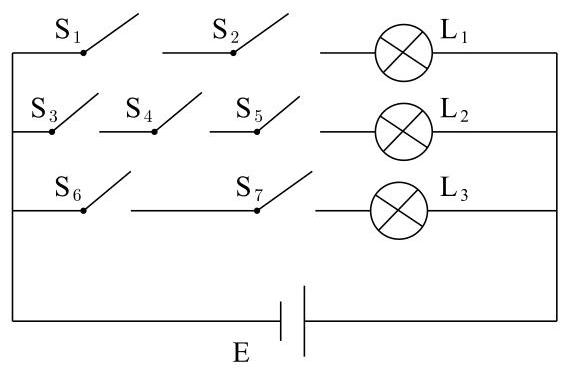
\includegraphics[max width=0.4\textwidth]{images/bo_d5jm9o77aajc7383vmi0_103_296_375_564_371_0.jpg}
\end{center}
\hspace*{3em} 

【答案】 \(\frac{27}{70}\)

【解析】 \({L}_{1}\) 最先亮起,可以根据最后亮起的灯分两种情形讨论.

情形一: \({L}_{2}\) 最后亮起.

\({L}_{2}\) 最后亮起等价于 \({S}_{3},{S}_{4},{S}_{5}\) 中的某一个开关恰在最后一个闭合,其概率为 \(\frac{3}{7}\) . 在此基础上， \({S}_{3},{S}_{4},{S}_{5}\) 中其余两个开关的闭合顺序对开灯顺序没有影响，可以将其剔除，只需考虑 \({S}_{1},{S}_{2}\) , \({S}_{6},{S}_{7}\) 的相对顺序.

现考虑 \({S}_{1},{S}_{2},{S}_{6},{S}_{7}\) 的闭合顺序. 要求 \({L}_{1}\) 先亮,即 \({L}_{3}\) 后亮,这等价于 \({S}_{6}\) 或 \({S}_{7}\) 最后一个亮起,概率为 \(\frac{1}{2}\) .

因此， \({L}_{2}\) 最后亮起且 \({L}_{1}\) 最先亮起的概率为 \(\frac{3}{7} \times  \frac{1}{2} = \frac{3}{14}\) .

情形二: \({L}_{3}\) 最后亮起.

\({L}_{3}\) 最后亮起等价于 \({S}_{6},{S}_{7}\) 中的某一个开关恰在最后一个闭合,其概率为 \(\frac{2}{7}\) .

在此基础上， \({S}_{6}\) ， \({S}_{7}\) 中剩下的那个开关的闭合顺序对开灯顺序没有影响，可以将其剔除，只需考虑 \({S}_{1},{S}_{2},{S}_{3},{S}_{4},{S}_{5}\) 的相对顺序.

现考虑 \({S}_{1},{S}_{2},{S}_{3},{S}_{4},{S}_{5}\) 的闭合顺序. 要求 \({L}_{1}\) 先亮,即 \({L}_{2}\) 后亮,这等价于 \({S}_{3},{S}_{4},{S}_{5}\) 中的某一个最后亮起,概率为 \(\frac{3}{5}\) .

因此, \({L}_{3}\) 最后亮起且 \({L}_{1}\) 最先亮起的概率为 \(\frac{2}{7} \times  \frac{3}{5} = \frac{6}{35}\) .

综上, \({L}_{1}\) 最先亮起的概率为 \(\frac{3}{14} + \frac{6}{35} = \frac{27}{70}\) .

备注: 设控制 \({L}_{1},{L}_{2},{L}_{3}\) 的开关数分别为 \({n}_{1},{n}_{2},{n}_{3}\) ,则 \({L}_{1}\) 最先亮起的概率为

\(\frac{{n}_{2}}{{n}_{1} + {n}_{2} + {n}_{3}} \cdot  \frac{{n}_{3}}{{n}_{1} + {n}_{3}} + \frac{{n}_{3}}{{n}_{1} + {n}_{2} + {n}_{3}} \cdot  \frac{{n}_{2}}{{n}_{1} + {n}_{2}} = \frac{\left( {2{n}_{1} + {n}_{2} + {n}_{3}}\right) {n}_{2}{n}_{3}}{\left( {{n}_{1} + {n}_{2} + {n}_{3}}\right) \left( {{n}_{1} + {n}_{2}}\right) \left( {{n}_{1} + {n}_{3}}\right) }\) .

2025 版上海高考真题及模拟训练合集(下册)

\section*{板块三: 中档主观题}

注:考试定位是第三道大题, 重点知识是条件概率、全概率公式、期望计算、方差计算 (包括概率中的和统计中的)、成对数据统计中的回归方程和卡方检验等,

“冷门知识”是加权方差公式(已考过)、正态分布的标准化(书上有例题,建议复习)、贝叶斯公式(书上打星号，理论上不会考)

\section*{1. 真题回顾}

【例题】1. (2025 上海春考) 甲、乙是两个体育社团的小组, 如下是两组组员身高的茎叶图 (单位: 厘米)，以身高的百位数和十位数作为 “茎” 排列在中间，个位数作为 “ 叶 ” 分列在两边.

(1)求甲、乙两组组员身高的第 60 百分位数；

(2)从甲、乙两组各选取一个组员，求两人身高均在 170 厘米以上的概率；

(3)为使两组人数相同，从甲组中调派一个队员到乙组. 是否存在甲组的一个组员，将他调派至乙组后, 甲、乙两组的平均身高都增大?

\begin{center}
\adjustbox{max width=\textwidth}{
\begin{tabular}{|c|c|c|c|c|c|c|c|c|c|c|c|c|c|c|}
\hline
\phantom{X} & \phantom{X} & \phantom{X} & \multicolumn{3}{|c|}{甲队} & \phantom{X} & \multicolumn{2}{|c|}{乙队} & \phantom{X} & \phantom{X} & \phantom{X} & \phantom{X} & \phantom{X} & \phantom{X} \\
\cline{1-15}
\phantom{X} & \phantom{X} & \phantom{X} & \phantom{X} & \phantom{X} & \phantom{X} & 15 & 9 & \phantom{X} & \phantom{X} & \phantom{X} & \phantom{X} & \phantom{X} & \phantom{X} & \phantom{X} \\
\cline{1-15}
\phantom{X} & 7 & 7 & 5 & 5 & 4 & 16 & 0 & 3 & 5 & 5 & 6 & 7 & 8 & 8 \\
\cline{1-15}
8 & 5 & 4 & 3 & 2 & 2 & 17 & 2 & \phantom{X} & \phantom{X} & \phantom{X} & \phantom{X} & \phantom{X} & \phantom{X} & \phantom{X} \\
\cline{1-15}
\phantom{X} & \phantom{X} & \phantom{X} & \phantom{X} & \phantom{X} & 3 & 18 & \phantom{X} & \phantom{X} & \phantom{X} & \phantom{X} & \phantom{X} & \phantom{X} & \phantom{X} & \phantom{X} \\
\cline{1-15}
\hline
\end{tabular}
}
\end{center}

【解析】(1) 甲队: \(\mathrm{i} = {12} \times  {60}\%  = {7.2}\) ,所以甲组的第 60 百分位数为第 8 项:173;

乙队: \(\mathrm{i} = {10} \times  {60}\%  = 6\) ,所以乙组的第 60 百分位数为第 6 项与 7 项的平均数: \(\frac{{166} + {167}}{2} =\) 166.5.

(2)记甲乙两队各选取一名组员，两人身高均 170 厘米以上为事件 \(A,P\left( A\right)  = \frac{\left| A\right| }{\left| \Omega \right| } = \frac{{C}_{7}^{1} \cdot  {C}_{1}^{1}}{{C}_{12}^{1} \cdot  {C}_{10}^{1}} \; = \frac{7}{120}\) .

(3) \(\bar{x} = {171.25}\) ， \(\bar{y} = {165.3}\) ，要使两组平均身高都增大，则从甲组调到乙组的数据 \(m\) 需满足 \({165.3} < m < {171.25}\) ,所以把甲组的其中一个 167 调到乙组即可.

【例题】2. (2024 上海秋考) 某地区为调查初中生体育锻炼时长与学业成绩的关系, 从该地区 29000 名初中生中抽取 580 人，得到日均体育锻炼时长 (表中简称“时长”) 与学业成绩的数据如下表所示:

\begin{center}
\adjustbox{max width=\textwidth}{
\begin{tabular}{|c|c|c|c|c|c|c|}
\hline
时长 & [0, 0.5) & [0.5,1) & [1,1.5) & [1.5,2) & [2,2.5) & 合计 \\
\cline{1-7}
优秀 & 5 & 44 & 42 & 3 & 1 & 95 \\
\cline{1-7}
不优秀 & 134 & 147 & 137 & 40 & 27 & 485 \\
\cline{1-7}
合计 & 139 & 191 & 179 & 43 & 28 & 580 \\
\cline{1-7}
\hline
\end{tabular}
}
\end{center}

(1)估计该地区 29000 名学生中日均锻炼时长不少于 1 小时的人数；

(2)估计该地区初中生的平均日均锻炼时长(精确到 0.1 小时);

(3)判断是否有 95\% 的把握认为该地区初中生学业成绩优秀与日均锻炼时长不少于 1 小时但少于 2 小时有关? 2025 版上海高考真题及模拟训练合集(下册)

\begin{center}
\adjustbox{max width=\textwidth}{
\begin{tabular}{|c|c|c|c|}
\hline
\phantom{X} & \(\lbrack 1,2)\) & 其他 & 合计 \\
\cline{1-4}
优秀 & \(a\) & \(b\) & \(a + b\) \\
\cline{1-4}
不优秀 & C & \(d\) & \(c + d\) \\
\cline{1-4}
合计 & \(a + c\) & \(b + d\) & \(a + b + c + d\) \\
\cline{1-4}
\hline
\end{tabular}
}
\end{center}

\({\chi }^{2} = \frac{n{\left( ad - bc\right) }^{2}}{\left( {a + b}\right) \left( {a + c}\right) \left( {b + d}\right) \left( {c + d}\right) }\) ,其中 \(n = a + b + c + d.\)

【解析】(1) 抽取的 580 人中,日均锻炼时长不少于 1 小时的人数为 \({179} + {43} + {28} = {250}\) 人,

所以估计该地区 29000 名学生中日均锻炼时长不少于 1 小时的人数

为 \({29000} \times  \frac{250}{580} = {12500}\) 人;

(2)估计该地区初中生的平均日均锻炼时长

为 \(\frac{1}{580}\left\lbrack  {\frac{0.5}{2} \times  {139} + \frac{{0.5} + 1}{2} \times  {191} + \frac{1 + {1.5}}{2} \times  {179} + \frac{{1.5} + 2}{2} \times  {43} + \frac{2 + {2.5}}{2} \times  {28}}\right\rbrack\)

\(\approx  {0.9}\) 小时;

(3) 列表:

\begin{center}
\adjustbox{max width=\textwidth}{
\begin{tabular}{|c|c|c|c|}
\hline
\phantom{X} & \(\lbrack 1,2)\) & 其他 & 合计 \\
\cline{1-4}
优秀 & 45 & 50 & 95 \\
\cline{1-4}
不优秀 & 177 & 308 & 485 \\
\cline{1-4}
合计 & 222 & 358 & 580 \\
\cline{1-4}
\hline
\end{tabular}
}
\end{center}

提出原假设 \({H}_{0}\) : 该地区初中生学业成绩优秀与日均锻炼时长不少于 1 小时

但少于 2 小时无关,

确定显著性水平 \(\alpha  = {0.05}\) ,

\({\chi }^{2} = \frac{{580} \times  {\left( {45} \times  {308} - {50} \times  {177}\right) }^{2}}{{95} \times  {485} \times  {222} \times  {358}} \approx  {3.976} > {3.841}\) ,否定原假设,

故有 95\% 的把握认为该地区初中生学业成绩优秀与日均锻炼时长

不少于 1 小时但少于 2 小时有关.

【例题】3. (2024上海春考)水果分为一级果和二级果, 共 136 箱, 其中一级果 102 箱, 二级果 34 箱.

(1)随机挑选两箱水果，求恰好一级果和二级果各一箱的概率;

(2)进行分层抽样，共抽 8 箱水果，求一级果和二级果各几箱；

(3)抽取若干箱水果，其中一级果共 120 个，单果质量平均数为 303.45 克，方差为 603.46；二级果 48 个, 单果质量平均数为 240.41 克, 方差为 648.21; 求 168 个水果的方差和平均数, 并预估果园中单果的质量.

【解析】(1)恰好一级果和二级果各一箱的概率 \(P = \frac{{C}_{102}^{1} \cdot  {C}_{34}^{1}}{{C}_{136}^{2}} = \frac{17}{45}\) ;

(2)一级果箱数二级果箱数 \(= 3 : 1\) ，共抽 8 箱水果，

因此一级果抽取 6 箱, 二级果抽取 2 箱.

(3)设一级果平均质量为 \(\bar{x}\) ，二级果质量为 \(\bar{y}\) ，总体样本平均质量为 \(\bar{z}\) ，

平均值 \(\bar{z} = \frac{{120}\bar{x} + {48}\bar{y}}{168} = {285.44}\) ,

方差 \({S}_{x}^{2} = \frac{1}{120}\sum {x}_{i}^{2} - {\left( \bar{x}\right) }^{2} \Rightarrow  \sum {x}_{i}^{2} = {120}\left( {{S}_{x}^{2} + {\left( \bar{x}\right) }^{2}}\right)\) ,

\({S}_{y}^{2} = \frac{1}{48}\sum {y}_{i}^{2} - {\left( \bar{y}\right) }^{2} \Rightarrow  \sum {y}_{i}^{2} = {48}\left( {{S}_{y}^{2} + {\left( \bar{y}\right) }^{2}}\right) ,\)

\({S}_{z}^{2} = \frac{1}{168}\sum {z}_{i}^{2} - {\left( \bar{z}\right) }^{2} = \frac{1}{168}\sum \left( {{x}_{i}^{2} + {y}_{i}^{2}}\right)  - {\left( \bar{z}\right) }^{2} = {1426.46},\)

平均质量 \(= \frac{{102}\bar{x} + {34}\bar{y}}{136} = {287.69}\) 克.

【例题】4. (2023 上海秋考)2023 年 6 月 7 日, 21 世纪汽车博览会在上海举行. 已知某汽车模型公司共有 25 个汽车模型, 其外观和内饰的颜色分布如下表所示:

\begin{center}
\adjustbox{max width=\textwidth}{
\begin{tabular}{|c|c|c|}
\hline
\phantom{X} & 红色外观 & 蓝色外观 \\
\cline{1-3}
棕色内饰 & 8 & 12 \\
\cline{1-3}
米色内饰 & 2 & 3 \\
\cline{1-3}
\hline
\end{tabular}
}
\end{center}

(1)若小明从这些模型中随机拿一个模型，记事件 \(A\) 为小明取到的模型为红色外观，事件 \(B\) 为小明取到的模型有棕色内饰. 求 \(P\left( B\right)\) 与 \(P\left( {B \mid  A}\right)\) ,并据此判断事件 \(A\) 和事件 \(B\) 是否独立;

(2)该公司举行了一个抽奖活动，并规定在一次抽奖中，每人可以一次性从这 25 个汽车模型中抽取两个，现有如下假设:

假设1:抽取的两个模型有三种结果:外观和内饰都相同、外观和内饰都不同、外观和内饰有且仅有一个相同;

假设2:按结果的可能性大小，概率越小奖金越高；

假设 3: 该抽奖活动的奖金额分别为:一等奖 600 元、二等奖 300 元、三等奖 150 元.

根据以上假设,设 \(X\) 为奖金额,请写出 \(X\) 的分布并求出 \(X\) 的数学期望.

【解析】(1) 由题意 \(P\left( A\right)  = \frac{8 + 2}{25} = \frac{2}{5},P\left( B\right)  = \frac{2 + 3}{25} = \frac{1}{5}\) ,

事件 \(A \cap  B\) ，即取到的汽车模型为红色且内饰为棕色，则 \(P\left( {A \cap  B}\right)  = \frac{2}{25}\) ，

所以 \(P\left( {B \mid  A}\right)  = \frac{P\left( {A \cap  B}\right) }{P\left( A\right) } = \frac{1}{5}\) ,

因为 \(P\left( A\right)  \cdot  P\left( B\right)  = \frac{2}{5} \times  \frac{1}{5} = \frac{2}{25} = P\left( {A \cap  B}\right)\) ,所以事件 \(A\text{ 、 }B\) 相互独立;

(2)外观和内饰均为同色的概率 \({P}_{1} = \frac{{C}_{8}^{2} + {C}_{12}^{2} + {C}_{2}^{2} + {C}_{3}^{2}}{{C}_{25}^{2}} = \frac{49}{150}\) ;

外观和内饰都异色的概率 \({P}_{2} = \frac{{C}_{8}^{1}{C}_{3}^{1} + {C}_{12}^{1}{C}_{2}^{1}}{{C}_{25}^{2}} = \frac{4}{25}\) ;

仅外观或仅内饰同色的概率 \({P}_{3} = \frac{{C}_{8}^{1}{C}_{2}^{1} + {C}_{12}^{1}{C}_{3}^{1} + {C}_{8}^{1}{C}_{12}^{1} + {C}_{2}^{1}{C}_{3}^{1}}{{C}_{25}^{2}} = \frac{77}{150}\) ;

所以 \({P}_{2} > {P}_{1} > {P}_{3}\) ,则一等奖对应 \({P}_{2}\) ,二等奖对应 \({P}_{1}\) ,三等奖对应 \({P}_{3}\) ,

所以 \(X\) 的分布为 \(\left( \begin{matrix} {600} & {300} & {150} \\  \frac{4}{25} & \frac{49}{150} & \frac{77}{150} \end{matrix}\right)\) ,

期望 \(E\left\lbrack  X\right\rbrack   = {600} \times  \frac{4}{25} + {300} \times  \frac{49}{150} + {150} \times  \frac{77}{150} = {271}\) (元). 2025 版上海高考真题及模拟训练合集(下册)

\section*{2. 模拟练习}

【练习】1. 在一个抽奖游戏中,主持人从编号为 1,2,3,4 的四个外观相同的空箱子中随机选择一个, 放入一件奖品，再将四个箱子关闭. 主持人知道奖品在哪个箱子里. 游戏规则是:主持人请抽奖人在这四个箱子中选择一个，然后主持人将随机打开其余三个箱子中的一个空箱子，并征询抽奖人是否改变选择. 现有抽奖人甲选择了 2 号箱, 于是主持人先打开了另外三个箱子中的一个空箱子,记为 \(X\) 号箱.

(1)求 \(X\) 的分布，期望和方差；

(2)若 \(X = 1\) ，如果你是抽奖人甲，请问你是坚持选 2 号箱，还是改选 3 号箱？

【解析】(1) 设 \({A}_{1}\text{ 、 }{A}_{2}\text{ 、 }{A}_{3}\text{ 、 }{A}_{4}\) 分别表示1,2,3,4号箱子里有奖品,

设 \({B}_{1}\text{ 、 }{B}_{2}\text{ 、 }{B}_{3}\text{ 、 }{B}_{4}\) 分别表示主持人打开1,2,3,4号箱子,

则 \(\Omega  = {A}_{1} \cup  {A}_{2} \cup  {A}_{3} \cup  {A}_{4}\) ,且 \({A}_{1}\text{ 、 }{A}_{2}\text{ 、 }{A}_{3}\text{ 、 }{A}_{4}\) 两两互斥,

由题意得事件 \({A}_{1}\text{ 、 }{A}_{2}\text{ 、 }{A}_{3}\text{ 、 }{A}_{4}\) 的概率都是 \(\frac{1}{4}\) ,

\(P\left( {{B}_{1} \mid  {A}_{4}}\right)  = \frac{1}{2},P\left( {{B}_{1} \mid  {A}_{2}}\right)  = \frac{1}{3},P\left( {{B}_{1} \mid  {A}_{3}}\right)  = \frac{1}{2},P\left( {{B}_{1} \mid  {A}_{1}}\right)  = 0,\)

由全概率公式,得 \(P\left( {B}_{1}\right)  = \mathop{\sum }\limits_{{i = 1}}^{4}P\left( {A}_{i}\right) P\left( {{B}_{1} \mid  {A}_{i}}\right)  = \frac{1}{4}\left( {\frac{1}{2} + \frac{1}{3} + \frac{1}{2}}\right)  = \frac{1}{3}\) ;

\(X = 1,3,4\) ,则 \(P\left( {X = 1}\right)  = \frac{1}{3}\) ,同理可得 \(P\left( {X = 3}\right)  = P\left( {X = 4}\right)  = \frac{1}{3}\) ,

故 \(X\) 的分布为

\begin{center}
\adjustbox{max width=\textwidth}{
\begin{tabular}{|c|c|c|c|}
\hline
\(X\) & 1 & 3 & 4 \\
\cline{1-4}
\(P\) & \(\frac{1}{3}\) & \(\frac{1}{3}\) & \(\frac{1}{3}\) \\
\cline{1-4}
\hline
\end{tabular}
}
\end{center}

所以 \(E\left( X\right)  = \frac{1}{3} + 3 \times  \frac{1}{3} + 4 \times  \frac{1}{3} = \frac{8}{3}\) ,

\(D\left( X\right)  = {\left( 1 - \frac{8}{3}\right) }^{2} \times  \frac{1}{3} + {\left( 3 - \frac{8}{3}\right) }^{2} \times  \frac{1}{3} + {\left( 4 - \frac{8}{3}\right) }^{2} \times  \frac{1}{3} = \frac{14}{9}\) ,

(2)在主持人打开 1 号箱的条件下， 4 号箱、 2 号箱、 3 号箱里有奖品的概率

分别为 \(P\left( {{A}_{4} \mid  {B}_{1}}\right)  = \frac{P\left( {{A}_{4} \cap  {B}_{1}}\right) }{P\left( {B}_{1}\right) } = \frac{P\left( {A}_{4}\right) P\left( {{B}_{1} \mid  {A}_{4}}\right) }{P\left( {B}_{1}\right) } = \frac{3}{8}\) ,

\(P\left( {{A}_{2} \mid  {B}_{1}}\right)  = \frac{P\left( {{A}_{2} \cap  {B}_{1}}\right) }{P\left( {B}_{1}\right) } = \frac{P\left( {A}_{2}\right) P\left( {{B}_{1} \mid  {A}_{2}}\right) }{P\left( {B}_{1}\right) } = \frac{1}{4},\)

\(P\left( {{A}_{3} \mid  {B}_{1}}\right)  = \frac{P\left( {{A}_{3} \cap  {B}_{1}}\right) }{P\left( {B}_{1}\right) } = \frac{P\left( {A}_{3}\right) P\left( {{B}_{1} \mid  {A}_{3}}\right) }{P\left( {B}_{1}\right) } = \frac{3}{8},\)

通过概率大小比较, 甲应该改选 4 号或 3 号箱.

【练习】2. (2024 届华二) 余山景区是国家 4A 级景区，其中“佘山天文台”和“佘山圣母大殿”景区的两张名片. 为了合理配置旅游资源,现对己游览“佘山天文台”景区且尚未游览“佘山圣母大殿” 景区的游客进行随机调查, 若不游览 “佘山圣母大殿” 景区记 2 分, 若继续游览 “佘山圣母大殿”景区记4分，假设每位游客选择游览“佘山圣母大殿”景区的概率均为 \(\frac{1}{3}\) ，游客之间选择意愿相互独立.

(1)从游客中随机抽取 2 人，记总得分为随机变量 \(X\) ，求 \(X\) 的数学期望；

(2)(i)记 \({p}_{k}\left( {k \in  {N}^{ * }}\right)\) 表示“从游客中随机抽取 \(k\) 人，总分恰为 \({2k}\) 分”的概率，求 \(\left\{  {p}_{k}\right\}\) 的前 4 项和;

(ii) 在对游客进行随机问卷调查中,记 \({a}_{n}\left( {n \in  {N}^{ * }}\right)\) 表示 “已调查过的累计得分恰为 \({2n}\) 分” 的概率,探求 \({a}_{n}\) 与 \({a}_{n - 1}\left( {n \geq  2}\right)\) 的关系,并求数列 \(\left\{  {a}_{n}\right\}\) 的通项公式.

【解析】(1) 易得 \(X\) 的所有取值为4,6,8,

因为每位游客选择游览“天下第一巷”景区的概率均为 \(\frac{1}{3}\) ,

游客之间选择意愿相互独立,

此时 \(P\left( {X = 4}\right)  = {\left( \frac{2}{3}\right) }^{2} = \frac{4}{9},P\left( {X = 6}\right)  = {C}_{2}^{1}\left( \frac{1}{3}\right) \left( \frac{2}{3}\right)  = \frac{4}{9},P\left( {X = 8}\right)  = {\left( \frac{1}{3}\right) }^{2} = \frac{1}{9}\) ,

所以 \(E\left( X\right)  = \frac{4}{9} \times  4 + \frac{4}{9} \times  6 + \frac{1}{9} \times  8 = \frac{48}{9} = \frac{16}{3}\) ;

(2)(i)易得“总分恰为 \({2k}\) 分”的概率为 \({\left( \frac{2}{3}\right) }^{k}\) ，

所以数列 \(\left\{  {p}_{k}\right\}\) 是以首项为 \(\frac{2}{3}\) ，公比为 \(\frac{2}{3}\) 的等比数列，

记该数列的前 \(n\) 项和为 \({S}_{n}\) ,则 \({S}_{4} = \frac{\frac{2}{3}\left\lbrack  {1 - {\left( \frac{2}{3}\right) }^{4}}\right\rbrack  }{1 - \frac{2}{3}} = \frac{130}{81}\) ;

(ii) 若“已调查过的累计得分恰为 \({2n}\) 分”的概率为 \({a}_{n}\) ,

此时得不到 \({2n}\) 分的情况只有先得 \({2n} - 2\) 分,再得 4 分,

概率为 \(\frac{1}{3}{a}_{n - 1}\left( {n \geq  2}\right) ,{a}_{1} = \frac{2}{3}\) ,所以 \(1 - {a}_{n} = \frac{1}{3}{a}_{n - 1}\) ,即 \({a}_{n} = 1 - \frac{1}{3}{a}_{n - 1}\) ,

此时 \({a}_{n} - \frac{3}{4} =  - \frac{1}{3}\left( {{a}_{n - 1} - \frac{3}{4}}\right)\) ,

则数列 \(\left\{  {{a}_{n} - \frac{3}{4}}\right\}\) 是以 \({a}_{1} - \frac{3}{4} =  - \frac{1}{12}\) 为首项, \(- \frac{1}{3}\) 为公比的等比数列,

所以 \({a}_{n} - \frac{3}{4} = \left( {{a}_{1} - \frac{3}{4}}\right)  \cdot  {\left( -\frac{1}{3}\right) }^{n - 1} =  - \frac{1}{12} \cdot  {\left( -\frac{1}{3}\right) }^{n - 1}\) ,故 \({a}_{n} = \frac{3}{4} + \frac{1}{4}{\left( -\frac{1}{3}\right) }^{n}\) .

【练习】3. (2024 届上中) 五月初, 某中学举行了“庆祝劳动光荣, 共绘五一华章”主题征文活动, 旨在通过文字的力量，展现劳动者的风采，传递劳动之美，弘扬劳动精神. 征文筛选由 \(A\) 、 \(B\) 、 \(C\) 三名老师负责. 首先由 \(A\) 、 \(B\) 两位老师对征文进行初审，若两位老师均审核通过，则征文通过筛选；若均审核不通过，则征文落选；若只有一名老师审核通过，则由老师 \(C\) 进行复审，复审合格才能通过筛选. 已知每篇征文通过 \(A\) 、 \(B\) 、 \(C\) 三位老师审核的概率分别为 \(\frac{3}{4}\) ， \(\frac{4}{5}\) ， \(\frac{3}{7}\) ，且各老师的审核互不影响.

(1)已知某篇征文通过筛选，求它经过了复审的概率；

(2)从投稿的征文中抽出 4 篇，设其中通过筛选的篇数为 \(X\) ，求 \(X\) 的分布和数学期望.

【解析】(1) 设事件 \(A = \{ A\) 老师审核通过 \(\}\) ,事件 \(B = \{ B\) 老师审核通过 \(\}\) ,

事件 \(C = \{ C\) 老师审核通过 \(\}\) ,

事件 \(D = \{\) 征文通过筛选 \(\}\) ,事件 \(E = \{\) 征文经过复审 \(\}\) ,

\(P\left( D\right)  = P\left( {A \cap  B}\right)  + P\left( {\bar{A} \cap  B \cap  C}\right)  + P\left( {A \cap  \bar{B} \cap  C}\right)\)

\(= \frac{3}{4} \times  \frac{4}{5} + \frac{1}{4} \times  \frac{4}{5} \times  \frac{3}{7} + \frac{3}{4} \times  \frac{1}{5} \times  \frac{3}{7} = \frac{3}{4}\) ,

\(P\left( {D \cap  E}\right)  = \frac{1}{4} \times  \frac{4}{5} \times  \frac{3}{7} + \frac{3}{4} \times  \frac{1}{5} \times  \frac{3}{7} = \frac{3}{20},P\left( {E \mid  D}\right)  = \frac{P\left( {D \cap  E}\right) }{P\left( D\right) } = \frac{1}{5}.\)

( 2 )由题意得 \(X \sim  B\left( {4,\frac{3}{4}}\right)\) ，则 \(X = 0,1,2,3,4,\) ，

\(P\left( {X = 0}\right)  = {C}_{4}^{0}{\left( \frac{1}{4}\right) }^{4} = \frac{1}{256},P\left( {X = 1}\right)  = {C}_{4}^{1}{\left( \frac{3}{4}\right) }^{1}{\left( \frac{1}{4}\right) }^{3} = \frac{12}{256} = \frac{3}{64},\) 2025 版上海高考真题及模拟训练合集(下册)

\(P\left( {X = 2}\right)  = {C}_{4}^{2}{\left( \frac{3}{4}\right) }^{2}{\left( \frac{1}{4}\right) }^{2} = \frac{54}{256} = \frac{27}{128},\)

\(P\left( {X = 3}\right)  = {C}_{4}^{3}{\left( \frac{3}{4}\right) }^{3}{\left( \frac{1}{4}\right) }^{1} = \frac{108}{256} = \frac{27}{64},P\left( {X = 4}\right)  = {C}_{4}^{4}{\left( \frac{3}{4}\right) }^{4} = \frac{81}{256},\)

\(X\) 的分布为 \(\left( \begin{matrix} 0 & 1 & 2 & 3 & 4 \\  \frac{1}{256} & \frac{3}{64} & \frac{27}{128} & \frac{27}{64} & \frac{81}{256} \end{matrix}\right)\)

\(E\left\lbrack  X\right\rbrack   = 4 \times  \frac{3}{4} = 3.\)

【练习】4. 为了检查一批零件的质量是否合格, 检查员计划从中依次随机抽取零件检查: 第 \(\mathrm{i}\) 次检查抽取 \(\mathrm{i}\) 号零件,测量其尺寸 \({y}_{i}\) (单位: 厘米). 检查员共进行了 100 次检查,整理并计算得到如下数据: \(\mathop{\sum }\limits_{{i = 1}}^{{100}}{y}_{i} = {52},\mathop{\sum }\limits_{{i = 1}}^{{100}}i{y}_{i} = {2428},\mathop{\sum }\limits_{{i = 1}}^{{100}}{y}_{i}^{2} = {30.18}\) .

(1)这批零件共有 1000 个. 若在抽查过程中，质量合格的零件共有 60 个，估计这批零件中质量合格的零件数量;

(2)若变量 \({y}_{i}\) 与 \(\mathrm{i}\) 存在线性关系，记 \({y}_{i} = \widehat{a}\mathrm{i} + \widehat{b}\) ，求回归系数 \(\widehat{a}\) 的值；

(3)在抽出的 100 个零件中，检查员计划从中随机抽出 20 个零件进行进一步检查，记抽出的 20 个零件中有 \(X\) 对相邻序号的零件. 求 \(X\) 的数学期望.

示例:零件序号为“1、2、4、5”与“1、2、3、5”时均恰有 2 对相邻序号的零件.

参考公式:

(1)线性回归方程: \(y = \widehat{a}x + \widehat{b}\) ，其中 \(\widehat{a} = \frac{\mathop{\sum }\limits_{{i = 1}}^{n}\left( {{x}_{i} - \bar{x}}\right) \left( {{y}_{i} - \bar{y}}\right) }{\mathop{\sum }\limits_{{i = 1}}^{n}{\left( {x}_{i} - \bar{x}\right) }^{2}},\widehat{b} = \bar{y} - \widehat{a}\bar{x}\) .

(2)期望的线性性质: \(E\left\lbrack  {\sum {X}_{i}}\right\rbrack   = \sum E\left\lbrack  {X}_{i}\right\rbrack\) ，其中 \({X}_{i}\) 是若干随机变量.

【解析】(1) 因为在这 100 个零件中,合格的零件为 60 个,

所以质量合格的零件所占样本比例为 \(\frac{60}{100} = \frac{3}{5}\) ,

而在这 1000 个零件中,质量合格的零件数为 \(\frac{3}{5} \times  {1000} = {600}\) (个);

(2) 由 \(\widehat{a} = \frac{\mathop{\sum }\limits_{{i = 1}}^{{100}}\left( {{x}_{i} - \bar{x}}\right) \left( {{y}_{i} - \bar{y}}\right) }{\mathop{\sum }\limits_{{i = 1}}^{{100}}{\left( {x}_{i} - \bar{x}\right) }^{2}}\) 得 \(\widehat{a} = \frac{\mathop{\sum }\limits_{{i = 1}}^{{100}}{y}_{i}i - {100}\bar{y}\bar{i}}{\mathop{\sum }\limits_{{i = 1}}^{{100}}{i}^{2} - {100}{\bar{i}}^{2}}\) ,

又因为 \(\mathop{\sum }\limits_{{i = 1}}^{{100}}{y}_{i} = {52},\mathop{\sum }\limits_{{i = 1}}^{{100}}i{y}_{i} = {2428},\mathop{\sum }\limits_{{i = 1}}^{{100}}{y}_{i}^{2} = {30.18}\) ,

所以 \(\bar{y} = \frac{\mathop{\sum }\limits_{{i = 1}}^{{100}}{y}_{i}}{100} = {0.52},\bar{i} = \frac{1 + 2 + \cdots  + {100}}{100} = {50.5}\) ,

所以 \(\widehat{a} = \frac{{2428} - {100} \times  {0.52} \times  {50.5}}{{338350} - {100} \times  {\left( {50.5}\right) }^{2}} =  - \frac{6}{2525}\) ;

(3) 用 \({X}_{i}\) 表示抽查的结果,若第 \(\mathrm{i}\) 个零件与第 \(\mathrm{i} + 1\) 个零件被选中,则记 \({X}_{i} = 1\) ,

若结果是其余情况,记 \({X}_{i} = 0\) ,则 \(X = {X}_{1} + {X}_{2} + \cdots  + {X}_{n}\) ,

由线性期望的性质得 \(E\left\lbrack  X\right\rbrack   = \mathop{\sum }\limits_{{i = 1}}^{{99}}E\left\lbrack  {X}_{i}\right\rbrack   = \mathop{\sum }\limits_{{i = 1}}^{{99}}P\left( {{X}_{i} = 1}\right)  = {99} \times  \frac{{C}_{98}^{18}}{{C}_{100}^{20}} = {3.8}\) 个.

【练习】5. (2025 届华二) 为了解某一地区电动汽车销售情况, 一机构根据统计数据, 用最小二乘法得

到电动汽车销量 \(y\) (单位:万台) 关于年份 \(x\) (单位:年) 的线性回归方程: \(y = {4.7x} - {9459.2}\) . 已知销量 \(y\) 的方差为 \({\sigma }_{y}^{2} = {50.8}\) ,年份 \(x\) 的方差为 \({\sigma }_{x}^{2} = 2\) .

(1) 求 \(y\) 与 \(x\) 的相关系数 (四舍五入到 0.001 )；

(2)该机构还调查了该地区 90 位购车车主的性别与购车种类情况，得到的数据如下表所示: 据此判断男、女车主在购买电动汽车一事上是否有显著差异；

\begin{center}
\adjustbox{max width=\textwidth}{
\begin{tabular}{|c|c|c|c|}
\hline
性别 & 购买非电动汽车 & 购买电动汽车 & 总计 \\
\cline{1-4}
男性 & 39 & 6 & 45 \\
\cline{1-4}
女性 & 30 & 15 & 45 \\
\cline{1-4}
总计 & 69 & 21 & 90 \\
\cline{1-4}
\hline
\end{tabular}
}
\end{center}

(3)在购买电动汽车的车主中按照性别进行分层抽样抽取 7 人，再从这 7 人中随机抽取 3 人， 记这 3 人中,男性的人数为 \(X\) ,求 \(X\) 的分布和期望.

附:回归方程系数 \(\widehat{a} = \frac{\mathop{\sum }\limits_{{i = 1}}^{n}\left( {{x}_{i} - \bar{x}}\right) \left( {{y}_{i} - \bar{y}}\right) }{\mathop{\sum }\limits_{{i = 1}}^{n}{\left( {x}_{i} - \bar{x}\right) }^{2}}\) ，相关系数 \(r = \frac{\mathop{\sum }\limits_{{i = 1}}^{n}\left( {{x}_{i} - \bar{x}}\right) \left( {{y}_{i} - \bar{y}}\right) }{\sqrt{\mathop{\sum }\limits_{{i = 1}}^{n}{\left( {x}_{i} - \bar{x}\right) }^{2}\mathop{\sum }\limits_{{i = 1}}^{n}{\left( {y}_{i} - \bar{y}\right) }^{2}}}\) ； \({\chi }^{2} = \frac{n{\left( ad - bc\right) }^{2}}{\left( {a + b}\right) \left( {c + d}\right) \left( {a + c}\right) \left( {b + d}\right) },P\left( {{\chi }^{2} \geq  {3.841}}\right)  \approx  {0.05}\) ,其中 \(n = a + b + c + d.\)

【解析】(1) 由回归方程系数与相关系数的公式, \(r = a \cdot  \frac{{\sigma }_{x}}{{\sigma }_{y}} \approx  {0.933}\) .

(2)把车主性别作为一个分类变量，是否购买电动汽车作为另一个分类变量.

提出原假设: 男、女车主在购买电动汽车一事上无显著差异.

确定显著性水平: \(\alpha  = {0.05}\) .

计算: \({\chi }^{2} = \frac{{90} \times  {\left( {39} \times  {15} - 6 \times  {30}\right) }^{2}}{{45} \times  {45} \times  {69} \times  {21}} \approx  {5.031}\) .

统计推断: 由 \(P\left( {{\chi }^{2} \geq  {3.841}}\right)  \approx  {0.05}\) ,而 \({\chi }^{2} \approx  {5.031} > {3.841}\) ,故否定原假设.

因此,男、女车主在购买电动汽车一事上有显著差异.

(3)由题意得 7 人中有 2 人为男性，5 人为女性.

\(X\) 的可能取值为 \(0\text{ 、 }1\text{ 、 }2\) .

所以 \(X\) 的分布为 \(\left( \begin{matrix} 0 & 1 & 2 \\  \frac{2}{7} & \frac{4}{7} & \frac{1}{7} \end{matrix}\right)\) ,进而得到 \(X\) 的期望 \(E\left\lbrack  X\right\rbrack   = \frac{6}{7}\) .

【注】第 (3) 问也可直接引用超几何分布的结论.

【练习】6. 张先生每周有 5 个工作日，工作日出行采用自驾方式，必经之路上有一个十字路口，直行车道有三条，直行车辆可以随机选择一条车道通行，记事件 \(A\) 为 “张先生驾车从左侧直行车道通行”.

(1)某日张先生驾车上班接近路口时，看到自己车前是一辆大货车，遂选择不与大货车从同一车道通行. 记事件 \(B\) 为 “大货车从中间直行车道通行”，求 \(P\left( {A \cap  B}\right)\) ；

(2)用 \(X\) 表示张先生每周工作日出行事件， \(A\) 发生的次数，求 \(X\) 的分布及期望 \(E\left\lbrack  X\right\rbrack\) .

【解析】(1) 法一:由题意得两辆车从直行车道通行这个样本空间中的基本事件共有 \({P}_{3}^{2}\) 个，

事件 \(A \cap  B\) 只有 1 个基本事件，

则 \(P\left( {A \cap  B}\right)  = \frac{1}{{P}_{3}^{2}} = \frac{1}{6}\) . 6 分

法二: 由题意得,事件 \(B\) 的概率为 \(P\left( B\right)  = \frac{1}{3}\) ,

事件 \(A\) 基于条件 \(B\) 的概率为 \(P\left( {A \mid  B}\right)  = \frac{1}{2},\cdots\) 4 分

则 \(P\left( {A \cap  B}\right)  = P\left( {A \mid  B}\right) P\left( B\right)  = \frac{1}{2} \times  \frac{1}{3} = \frac{1}{6}\) . 6 分

(2) 由题意得,事件 \(A\) 发生的次数 \(X\) 可取0,1,2,3,4,5

则 \(X\) 的分布为

\begin{center}
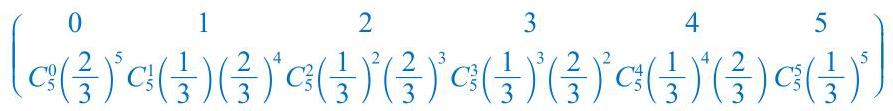
\includegraphics[max width=0.7\textwidth]{images/bo_d5jm9o77aajc7383vmi0_111_289_593_893_111_0.jpg}
\end{center}
\hspace*{3em} 

即 \(\left( \begin{matrix} 0 & 1 & 2 & 3 & 4 & 5 \\  {32} & 8 & {80} & {40} & 1 & 0 \\  {243} & {243} & {243} & {243} & {243} & {243} \end{matrix}\right)\) , 4.

则 \(E\left\lbrack  X\right\rbrack   = 1 \times  \frac{80}{243} + 2 \times  \frac{80}{243} + 3 \times  \frac{40}{243} + 4 \times  \frac{10}{243} + 5 \times  \frac{1}{243},\cdots\) 6 分

则所求的 \(X\) 的期望 \(E\left\lbrack  X\right\rbrack   = \frac{5}{3}\) . 8 分

【练习】7. 在对一些敏感性问题进行统计调查时,会对问卷进行“敏感信息脱敏”设计. 例如调查马路上没什么行驶车辆时是否会有乱穿马路行为，为了消除被调查者的顾虑，使他们能够如实回答问题，对问卷进行了特殊设计以达到 “敏感信息脱敏”效果:调查中设置了两个问题: \circled{1}  你是否为男生？ \circled{2} 你是否有过乱穿马路行为.

调查分两个环节, 第一个环节: 确定回答的问题, 让被调查者从装有 3 个红球, 3 个黑球 (除颜色外完全相同) 的袋子中随机摸取两个球, 摸到同色两球的学生如实回答第一个问题, 摸到异色两球的学生如实回答第二个问题. 第二个环节:填写问卷 (问卷中只有“是”与“否”两个选项). 对问卷进行统计, 有 70 张答案为“是”.

(1)根据以上的调查结果, 利用你所学的知识, 估计该校中学生有乱穿马路行为的概率;

(2)据核实，以上的 300 名学生中有 20 名学生在考试中有乱传马路行为，其中男生 15 人，女生 5 人，试判断是否有 97.5\% 的把握认为中学生在考试中有无乱传马路行为与性别有关.

参考公式和数据如下: \({K}^{2} = \frac{n{\left( ad - bc\right) }^{2}}{\left( {a + b}\right) \left( {c + d}\right) \left( {a + c}\right) \left( {b + d}\right) },n = a + b + c + d\) .

\begin{center}
\adjustbox{max width=\textwidth}{
\begin{tabular}{|c|c|c|c|c|c|}
\hline
\(P\left( {{K}^{2} \geq  {k}_{0}}\right)\) & 0.15 & 0.10 & 0.05 & 0.025 & 0.005 \\
\cline{1-6}
\({k}_{0}\) & 2.072 & 2.706 & 3.841 & 5.024 & 7.879 \\
\cline{1-6}
\hline
\end{tabular}
}
\end{center}

【解析】(1) 因为摸到同色两球的概率 \(P = \frac{{C}_{3}^{2} + {C}_{3}^{2}}{{C}_{6}^{2}} = \frac{2}{5}\) ,

所以回答第一个问题的人数为 \({300} \times  \frac{2}{5} = {120}\) ,回答第二个问题的人数为 180,

因为男女人数相等，是等可能的，

所以回答第一个问题，选择“是”的同学人数为 \({120} \times  \frac{1}{2} = {60}\) ,

则回答第二个问题，选择“是”的同学人数为 10 ，

所以估计中学生在考试中有乱传马路行为的概率为 \(\frac{10}{180} = \frac{1}{18}\) ;

(2)2×2 列联表如下: 2025 版上海高考真题及模拟训练合集(下册)

\begin{center}
\adjustbox{max width=\textwidth}{
\begin{tabular}{|c|c|c|c|}
\hline
\phantom{X} & 男生 & 女生 & 合计 \\
\cline{1-4}
有乱传马路行为 & 15 & 5 & 20 \\
\cline{1-4}
没有乱传马路行为 & 135 & 145 & 280 \\
\cline{1-4}
合计 & 150 & 150 & 300 \\
\cline{1-4}
\hline
\end{tabular}
}
\end{center}

因为 \({K}^{2} = \frac{{300} \times  {\left( {15} \times  {145} - 5 \times  {135}\right) }^{2}}{{150} \times  {150} \times  {20} \times  {280}} = \frac{75}{14} \approx  {5.357} > {5.024}\) ,

所以有 97.5\% 的把握认为中学生在考试中有无乱传马路行为与性别有关.

【练习】8. 某高中举行了一次知识竞赛. 为了了解本次竞赛成绩情况, 从中抽取了部分学生的成绩作为样本进行统计. 将成绩进行整理后,依次分为五组 \(\left( {\lbrack {50},{60}}\right) \text{ 、 }\lbrack {60},{70})\text{ 、 }\lbrack {70},{80})\text{ 、 }\lbrack {80}\) , 90)、[90,100]，其中第 1 组的频率为第 2 组和第 4 组频率的等比中项. 请根据下面的频率分布直方图(如图所示)解决下列问题:

(1) 求 \(a\) 、 \(b\) 的值；

(2)从样本数据在 \(\lbrack {50},{60}),\lbrack {70},{80})\) 两个小组内的学生中，用分层抽样的方法抽取 7 名学生， 再从这 7 名学生中随机选出 2 人，求选出的两人恰好来自不同小组的概率；

(3)某老师在此次竞赛成绩中抽取了 10 名学生的分数: \({x}_{1},{x}_{2},{x}_{3},\cdots ,{x}_{10}\) ，已知这 10 个分数的平均数 \(\bar{x} = {88}\) ，方差 \({s}^{2} = {25}\) ，若剔除其中的 95 和 81 两个分数，求剩余 8 个分数的平均数与方差.

【解析】(1) 由 \({0.16}^{2} = {0.08}\left( {10a}\right)\) ,解得 \(a = {0.032},\cdots \cdots 2\) 分

又 \(\left( {{0.008} + {0.016} + {0.032} + {0.04} + b}\right)  \times  {10} = 1\) ,解得 \(b = {0.004},\cdots\)

所以 \(a = {0.032},b = {0.004}\) .

(2)按分层抽样法,两层应分别抽取 2 人和 5 人，……6 分

事件 \(A\) : “抽到的两位同学来自不同小组”,所以 \(P\left( A\right)  = \frac{{C}_{2}^{1}{C}_{5}^{1}}{{C}_{7}^{2}} = \frac{10}{21}\cdots \cdots 8\) 分

(3) 因为 \(\bar{x} = {88},{x}_{1} + {x}_{2} + \cdots  + {x}_{10} = {10} \times  {88} = {880}\) ,

所以 \({s}^{2} = \frac{1}{10}\left\lbrack  {{\left( {x}_{1} - \bar{x}\right) }^{2} + {\left( {x}_{2} - \bar{x}\right) }^{2} + \cdots  + {\left( {x}_{10} - \bar{x}\right) }^{2}}\right\rbrack\)

\(= \frac{1}{10}\left\lbrack  {{x}_{1}^{2} + {x}_{2}^{2} + \cdots  + {x}_{10}^{2} - 2\left( {{x}_{1} + {x}_{2} + \cdots  + {x}_{10}}\right) \bar{x} + {10}{\bar{x}}^{2}}\right\rbrack\)

\begin{center}
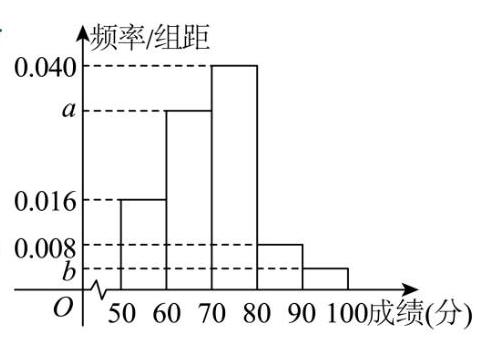
\includegraphics[max width=0.4\textwidth]{images/bo_d5jm9o77aajc7383vmi0_112_975_1506_478_341_0.jpg}
\end{center}
\hspace*{3em} 

\(= \frac{1}{10}\left( {{x}_{1}^{2} + {x}_{2}^{2} + \cdots  + {x}_{10}^{2} - {20}{\bar{x}}^{2} + {10}\bar{x}}\right)  = \frac{1}{10}\left( {{x}_{1}^{2} + {x}_{2}^{2} + \cdots }\right.\)

\(\left. {+{x}_{10}^{2}}\right)  - {\bar{x}}^{2}\)

\(= \frac{1}{10}\left( {{x}_{1}^{2} + {x}_{2}^{2} + \cdots  + {x}_{10}^{2}}\right)  - {88}^{2} = {5}^{2},\)

所以 \({x}_{1}^{2} + {x}_{2}^{2} + \cdots  + {x}_{10}^{2} = {77690},\cdots \cdots {10}\) 分

剔除其中的 95 和 81 两个数，设剩余 8 个数为 \({x}_{1},{x}_{2} \; {x}_{3},\cdots ,{x}_{8},\)

平均数与标准差分别为 \(\overline{{x}_{0}},{s}_{0}\) ,

则剩余 8 个数的平均数 \(\overline{{x}_{0}} = \frac{{x}_{1} + {x}_{2} + {x}_{3} + \cdots  + {x}_{8}}{8}\)

\(= \frac{{880} - {95} - {81}}{8} = {88},\)

方差 \({s}_{0}^{2} = \frac{1}{8}\left\lbrack  {{\left( {x}_{1} - \overline{{x}_{0}}\right) }^{2} + {\left( {x}_{2} - \overline{{x}_{0}}\right) }^{2} + \cdots  + {\left( {x}_{8} - \overline{{x}_{0}}\right) }^{2}}\right\rbrack\)

\[
= \frac{1}{8}\left( {{x}_{1}^{2} + {x}_{2}^{2} + \cdots  + {x}_{8}^{2}}\right)  - {88}^{2} = \frac{1}{8}\left( {{77690} - {95}^{2} - {81}^{2}}\right)  - {88}^{2} = {19}\cdots \cdots {14}
\]

【练习】9. 在传染病学中, 通常把从致病刺激物侵入机体或者对机体发生作用起, 到机体出现反应或开始呈现该疾病对应的相关症状时止的这一阶段称为潜伏期. 一研究团队统计了某地区 1000 名患者的相关信息，得到如下表格:

\begin{center}
\adjustbox{max width=\textwidth}{
\begin{tabular}{|c|c|c|c|c|c|c|c|}
\hline
潜伏期(单位:天) & [0,2] & (2,4] & (4,6] & (6,8] & (8,10] & (10,12] & (12,14] \\
\cline{1-8}
人数 & 50 & 150 & 200 & 300 & 200 & 60 & 40 \\
\cline{1-8}
\hline
\end{tabular}
}
\end{center}

(1)求这 1000 名患者的潜伏期的样本平均数值 \(\bar{x}\) (同一组中的数据用该组区间的中点值作代表, 结果四舍五入为整数);

(2)该传染病的潜伏期受诸多因素的影响，为研究潜伏期与患者年龄的关系，以潜伏期是否超过 8 天为标准进行分层抽样，从上述 1000 名患者中抽取 200 人，得到如下列联表，请将列联表补充完整，并根据列联表判断，能否在犯错误的概率不超过 5\% 的前提下，认为潜伏期与患者年龄有关；

\begin{center}
\adjustbox{max width=\textwidth}{
\begin{tabular}{|c|c|c|c|}
\hline
\phantom{X} & 潜伏期≤8天 & 潜伏期>8天 & 总计 \\
\cline{1-4}
50 岁以上(含 50) & \phantom{X} & \phantom{X} & 100 \\
\cline{1-4}
50 岁以下 & 65 & \phantom{X} & \phantom{X} \\
\cline{1-4}
总计 & \phantom{X} & \phantom{X} & 200 \\
\cline{1-4}
\hline
\end{tabular}
}
\end{center}

(3) 以这 1000 名患者的潜伏期超过 8 天的频率，代替该地区 1 名患者潜伏期超过 8 天的概率， 每名患者的潜伏期是否超过 8 天相互独立. 为了深入研究，该研究团队随机调查了 20 名患者，其中潜伏期超过 8 天的人数最有可能(即概率最大)是多少？

附: \({\chi }^{2} = \frac{n{\left( ad - bc\right) }^{2}}{\left( {a + b}\right) \left( {c + d}\right) \left( {a + c}\right) \left( {b + d}\right) }\) ,其中 \(n = a + b + c + d\) .

\begin{center}
\adjustbox{max width=\textwidth}{
\begin{tabular}{|c|c|c|c|}
\hline
\(P\left( {{\chi }^{2} \geq  {k}_{0}}\right)\) & 0.05 & 0.025 & 0.010 \\
\cline{1-4}
\({k}_{0}\) & 3.841 & 5.024 & 6.635 \\
\cline{1-4}
\hline
\end{tabular}
}
\end{center}

【解析】(1) \(\bar{x} = 1 \times  \frac{50}{1000} + 3 \times  \frac{150}{1000} + 5 \times  \frac{200}{1000} + 7 \times  \frac{300}{1000} + 9 \times  \frac{200}{1000} + {11} \times  \frac{60}{1000}\)

\(+ {13} \times  \frac{40}{1000} = \frac{6580}{1000} = {6.58} \approx  7\) (天).

(2)潜伏期天数在 \(\left\lbrack  {0,8}\right\rbrack\) 的频率为 \(\frac{{50} + {150} + {200} + {300}}{1000} = {0.7}\) ，

潜伏期天数在 \((8,{14}\rbrack\) 的频率为 0.3 ,

故 200 人中潜伏期在 \(\left\lbrack  {0,8}\right\rbrack\) 的有 \({200} \times  {0.7} = {140}\) 人，在 \((8,{14}\rbrack\) 的有 60 人，

补充完整的 \(2 \times  2\) 列联表如下:

\begin{center}
\adjustbox{max width=\textwidth}{
\begin{tabular}{|c|c|c|c|}
\hline
\phantom{X} & 潜伏期≤8天 & 潜伏期>8天 & 总计 \\
\cline{1-4}
50 岁以上(含50) & 75 & 25 & 100 \\
\cline{1-4}
50 岁以下 & 65 & 35 & 100 \\
\cline{1-4}
总计 & 140 & 60 & 200 \\
\cline{1-4}
\hline
\end{tabular}
}
\end{center}

所以 \({\chi }^{2} = \frac{{200} \times  {\left( {75} \times  {35} - {65} \times  {25}\right) }^{2}}{{100} \times  {100} \times  {140} \times  {60}} = \frac{50}{21} \approx  {2.381} < {3.841}\) ,

故不能在犯错误的概率不超过 5\% 的前提下，认为潜伏期与患者年龄有关.

(3)由题意得一名患者潜伏期超过 8 天的概率为 \(\frac{300}{1000} = \frac{3}{10}\) ，

设 20 名患者中潜伏期超过 8 天的人数为 \(X\) ,则 \(X \sim  B\left( {{20},\frac{3}{10}}\right)\) ,

所以 \(P\left( {X = k}\right)  = {C}_{20}^{k}{\left( \frac{7}{10}\right) }^{{20} - k}{\left( \frac{3}{10}\right) }^{k}\) ,且 \(0 \leq  k \leq  {20},k \in  N\) ,

由题意得 \(\left\{  \begin{array}{ll} P\left( {X = k}\right)  \geq  P & \left( {X = k + 1}\right) \\  P\left( {X = k}\right)  \geq  P & \left( {X = k - 1}\right)  \end{array}\right.\) ,

即 \(\left\{  \begin{array}{l} {C}_{20}^{k}{\left( \frac{7}{10}\right) }^{{20} - k}{\left( \frac{3}{10}\right) }^{k} \geq  {C}_{20}^{k + 1}{\left( \frac{7}{10}\right) }^{{19} - k}{\left( \frac{3}{10}\right) }^{k + 1} \\  {C}_{20}^{k}{\left( \frac{7}{10}\right) }^{{20} - k}{\left( \frac{3}{10}\right) }^{k} \geq  {C}_{20}^{k - 1}{\left( \frac{7}{10}\right) }^{{21} - k}{\left( \frac{3}{10}\right) }^{k - 1} \end{array}\right.\) ,化简得 \(\left\{  \begin{array}{l} 7\left( {k + 1}\right)  \geq  3\left( {{20} - k}\right) \\  3\left( {{21} - k}\right)  \geq  {7k} \end{array}\right.\) ,

解得 \(\frac{53}{10} \leq  k \leq  \frac{63}{10}\) ,故 \(k = 6\) ,即潜伏期超过 8 天的人数最有可能是 6 .

【练习】10. 某企业准备把一种新型零件交给甲工厂或乙工厂生产. 经过试生产, 质检人员抽样发现: 甲工厂试生产的一批零件的合格率为 90\%，乙工厂试生产的另一批零件的合格率为 96\%；若将这两批零件混合放在一起，则合格率为 94\%.

(1)从混合放在一起的零件中随机抽取 3 个. 用频率估计概率，记这 3 个零件中来自甲工厂的个数为 \(X\) ,求随机变量 \(X\) 的分布和期望;

(2)为了争取获得该零件的生产订单，甲工厂提高了生产该零件的质量指标. 已知在甲工厂提高质量指标的条件下, 该企业把零件交给甲工厂生产的概率, 大于在甲工厂不提高质量指标的条件下, 该企业把零件交给甲工厂生产的概率.

用事件 \(A\) 表示 “甲工厂提高了生产该零件的质量指标”, 事件 \(B\) 表示 “该企业把零件交给甲工厂生产”. 已知 \(0 < P\left( B\right)  < 1\) ，求证: \(P\left( {A \mid  B}\right)  > P\left( {A \mid  \bar{B}}\right)\) .

【解析】(1) 设来自甲工厂的零件有 \(m\) 件,来自乙工厂零件有 \(n\) 件.

从混合放在一起的零件中任取一件,

用事件 \(C\) 表示“零件是合格品”,事件 \(M\) 表示“零件来自甲工厂”,

则 \(P\left( C\right)  = P\left( {C \mid  M}\right) P\left( M\right)  + P\left( {C \mid  \bar{M}}\right) P\left( \bar{M}\right)\) 2 分

\(= {90}\%  \cdot  \frac{m}{m + n} + {96}\%  \cdot  \frac{n}{m + n} = {94}\%\) ,

解得 \(n = {2m}\) ，故 \(P\left( M\right)  = \frac{1}{3}\) . 4 分

由题意得随机变量 \(X \sim  B\left( {3,\frac{1}{3}}\right)\) ,

得 \(X\) 的分布为 \(\left( \begin{matrix} 0 & 1 & 2 & 3 \\  \frac{8}{27} & \frac{4}{9} & \frac{2}{9} & \frac{1}{27} \end{matrix}\right)\) , 6 分

\(E\left\lbrack  X\right\rbrack   = 3 \times  \frac{1}{3} = 1.\) 8 分

(2)由题意得 \(P\left( {B \mid  A}\right)  > P\left( {B \mid  \bar{A}}\right)\) ， 10 分

即 \(\frac{P\left( {A \cap  B}\right) }{P\left( A\right) } > \frac{P\left( {\bar{A} \cap  B}\right) }{P\left( \bar{A}\right) }\) ,

由于 \(P\left( A\right)  > 0,P\left( \bar{A}\right)  > 0\) ,故 \(P\left( {A \cap  B}\right) P\left( \bar{A}\right)  > P\left( {\bar{A} \cap  B}\right) P\left( A\right)\) .

由于 \(P\left( \bar{A}\right)  = 1 - P\left( A\right) ,P\left( {\bar{A} \cap  B}\right)  = P\left( B\right)  - P\left( {A \cap  B}\right)\) ,

代入上式得 \(P\left( {A \cap  B}\right) \left( {1 - P\left( A\right) }\right)  > \left( {P\left( A\right)  - P\left( {A \cap  B}\right) }\right) P\left( A\right)\) ,

整理得 \(P\left( {A \cap  B}\right)  > P\left( A\right) P\left( B\right)\) . 12 分

进而有 \(P\left( {A \cap  B}\right) \left( {1 - P\left( B\right) }\right)  > \left( {P\left( A\right)  - P\left( {A \cap  B}\right) }\right) P\left( B\right)\) ,

即 \(P\left( {A \cap  B}\right) P\left( \bar{B}\right)  > P\left( {A \cap  \bar{B}}\right) P\left( B\right)\) .

由于 \(P\left( B\right)  > 0,P\left( \bar{B}\right)  > 0\) ,得 \(\frac{P\left( {A \cap  B}\right) }{P\left( B\right) } > \frac{P\left( {A \cap  \bar{B}}\right) }{P\left( \bar{B}\right) }\) ,

即 \(P\left( {A \mid  B}\right)  > P\left( {A \mid  \bar{B}}\right)\) . 14 分

\section*{10 十、建模与应用题}

注: 占的位置应该是 11 题或者 15 题, 其实难度是很低的

\section*{板块一:中档客观题}

\section*{1. 真题回顾}

\begin{center}
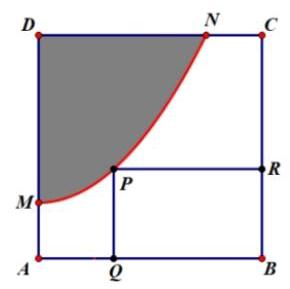
\includegraphics[max width=0.2\textwidth]{images/bo_d5jm9o77aajc7383vmi0_116_1152_491_290_289_0.jpg}
\end{center}
\hspace*{3em} 

【例题】1. (2025 上海春考) 如图所示,正方形 \({ABCD}\) 是一块边长为 4 的工程用料，阴影部分所示是被腐蚀的区域，其余部分完好. 曲线 \({MN}\) 是以 \({AD}\) 为对称轴的抛物线的一部分, \({MD} = {ND} = 3\) . 工人要从完好的工程原料中截取一块最大的矩形, 则这块矩形原料的面积最大时， \({AQ}\) 的长度是\_\_\_\_\_ (精确到 0.1 ).

【答案】 2.2

【解析】以点 \(A\) 为坐标原点,建立平面直角坐标系,则 \(M\left( {0,1}\right) ,N\left( {3,4}\right)\) . 设抛物线 \({MN}\) 的方程为 \(y = a{x}^{2} + 1\) ，将 \(N\left( {3,4}\right)\) 代入解得 \(a = \frac{1}{3}\) .

设点 \(P\left( {x,\frac{1}{3}{x}^{2} + 1}\right)\) ,则 \({PQ} = \frac{1}{3}{x}^{2} + 1,{PR} = 4 - x\) ,

所以矩形 \({BPRQ}\) 的面积 \(f\left( x\right)  = {PQ} \cdot  {PR} = \left( {\frac{1}{3}{x}^{2} + 1}\right) \left( {4 - x}\right)  =  - \frac{1}{3}{x}^{3} + \frac{4}{3}{x}^{2} - x + 4\) .

所以 \({f}^{\prime }\left( x\right)  =  - {x}^{2} + \frac{8}{3}x - 1\) ,令 \({f}^{\prime }\left( x\right)  = 0\) ,解得 \(x = \frac{4 \pm  \sqrt{7}}{3}\) .

检验可知 \(x = \frac{4 + \sqrt{7}}{3}\) 时, \(y = f\left( x\right)\) 取得极大值 (最大值),此时 \({AQ} = x = \frac{4 + \sqrt{7}}{3} \approx  {2.2}\) .

\begin{center}
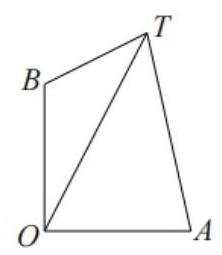
\includegraphics[max width=0.2\textwidth]{images/bo_d5jm9o77aajc7383vmi0_116_1221_1182_222_255_0.jpg}
\end{center}
\hspace*{3em} 

【例题】2. (2024 上海秋考) 海上有灯塔 \(O,A,B\) 和船只 \(T,A\) 在 \(O\) 的正东方向, \(B\) 在 \(O\) 的正北方向, \(A,B\) 到 \(O\) 的距离相同, \(O,A,T,B\) 按逆时针排列. 若 \(\angle {OTA} = {37.0}^{ \circ  },\angle {OTB} = {16.5}^{ \circ  }\) ,则 \(\angle {BOT} =\) \_\_\_\_\_ (精确到 \({0.1}^{ \circ  }\) ).

【答案】 \(\angle {BOT} = {7.8}^{ \circ  }\)

【解析】设 \(\angle {BOT} = \theta ,\angle {AOT} = {90}^{ \circ  } - \theta\) ,

在 \(\bigtriangleup {AOT}\) 中,由正弦定理得 \(\frac{OT}{\sin A} = \frac{OA}{\sin \angle {OTA}}\) ,即 \(\angle {OTA} = {37.0}^{ \circ  },\angle {OTB} = \; {16.5}^{ \circ  }\) ,

在 \(\bigtriangleup {BOT}\) 中，由正弦定理得 \(\frac{OT}{\sin B} = \frac{OB}{\sin \angle {OTB}}\) ，即 \(\frac{OT}{\sin \left( {\theta  + {16.5}^{ \circ  }}\right) } = \frac{OB}{\sin {16.5}^{ \circ  }}\) ，

因为 \({OA} = {OB}\) ,两式相除,得 \(\frac{\sin \left( {{90}^{ \circ  } - \theta  + {37.0}^{ \circ  }}\right) }{\sin \left( {\theta  + {16.5}^{ \circ  }}\right) } = \frac{\sin {37.0}^{ \circ  }}{\sin {16.5}^{ \circ  }}\left( *\right)\) ,

所以 \(\frac{\cos \theta \cos {37.0}^{ \circ  } + \sin \theta \sin {37.0}^{ \circ  }}{\sin \theta \cos {16.5}^{ \circ  } + \cos \theta \sin {16.5}^{ \circ  }} = \frac{\sin {37.0}^{ \circ  }}{\sin {16.5}^{ \circ  }}\) ,

所以 \(\frac{\cos {37.0}^{ \circ  } + \tan \theta \sin {37.0}^{ \circ  }}{\tan \theta \cos {16.5}^{ \circ  } + \sin {16.5}^{ \circ  }} = \frac{\sin {37.0}^{ \circ  }}{\sin {16.5}^{ \circ  }}\) ,

所以 \(\cos {37.0}^{ \circ  }\sin {16.5}^{ \circ  } + \tan \theta \sin {37.0}^{ \circ  }\sin {16.5}^{ \circ  }\)

\(= \tan \theta \sin {37.0}^{ \circ  }\cos {16.5}^{ \circ  } + \sin {37.0}^{ \circ  }\sin {16.5}^{ \circ  }\) ,

所以 \(\tan \theta \left( {\sin {37.0}^{ \circ  }\cos {16.5}^{ \circ  } - \sin {37.0}^{ \circ  }\sin {16.5}^{ \circ  }}\right)\)

\(= \cos {37.0}^{ \circ  }\sin {16.5}^{ \circ  } - \sin {37.0}^{ \circ  }\sin {16.5}^{ \circ  }\) ,

所以 \(\tan \theta  = \frac{\cos {37.0}^{ \circ  }\sin {16.5}^{ \circ  } - \sin {37.0}^{ \circ  }\sin {16.5}^{ \circ  }}{\sin {37.0}^{ \circ  }\cos {16.5}^{ \circ  } - \sin {37.0}^{ \circ  }\sin {16.5}^{ \circ  }} = \frac{\cot {37.0}^{ \circ  } - 1}{\cot {16.5}^{ \circ  } - 1}\) ,

由计算器得 \(\theta  \approx  {7.8}^{ \circ  }\) .

【注】以上看起来繁琐只是因为把具体化简过程写了出来,事实上,在 \(\left( *\right)\) 中,可以直接对角相

2025 版上海高考真题及模拟训练合集(下册)

乘后, 按计算器出近似值.

【例题】3. (2024上海春考)某正方形景区 \({ABCD}\) 边长为 \({1.2}\mathrm{\;{km}}\) ，点 \(E\) 距 \({AB}\) 、 \({AD}\) 的距离都为 \({0.2}\mathrm{\;{km}}\) ,点 \(F\) 距 \({BC}\text{ 、 }{CD}\) 的距离都为 \({0.4}\mathrm{\;{km}}\) ,现要在景区内建一条圆形交通轨道 (不计宽度),要使轨道经过 \(E\text{ 、 }F\) 两点,且与 \({AD}\) 边有一个公共点以便作为出入口，则这条圆形交通轨道的周长为\_\_\_\_\_ (精确到 \({0.01}\mathrm{\;{km}}\) ).

\begin{center}
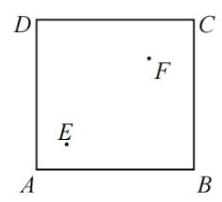
\includegraphics[max width=0.2\textwidth]{images/bo_d5jm9o77aajc7383vmi0_117_1227_307_222_202_0.jpg}
\end{center}
\hspace*{3em} 

【答案】 2.73km

【解析】以 \(A\) 为原点建系, \(E\left( {{0.2},{0.2}}\right) ,F\left( {{0.8},{0.8}}\right)\) ,

直线 \({EF}\) 中垂线 \(y - {0.5} =  - \left( {x - {0.5}}\right)\) ,化简得 \(y =  - x + 1\) ,

所以圆心为 \(\left( {t, - t + 1}\right)\) ,半径为 \(t\) ,且经过 \(E,F\) 点,

即 \({\left( t - {0.2}\right) }^{2} + {\left( -t + 1 - {0.2}\right) }^{2} = {t}^{2}\) ,化简得 \({t}^{2} - {2t} + {0.68} = 0\) ,解得 \(t = \frac{5 - 2\sqrt{2}}{5}\)

所以周长 \({2\pi t} \approx  {2.73}\mathrm{\;{km}}\) .

【例题】4. (2023 上海秋考) 某公园欲建设一段斜坡，假设斜坡底端在水平地面上且坡面笔直，斜坡顶端距水平地面的高度为 4 米,斜坡与水平地面的夹角为 \(\theta\) . 已知游客从坡底沿着斜坡每向上走 1 米，消耗的体力为 (1.025 - cos内，若要使游客从斜坡底端走到斜坡顶端所消耗的体力最少，则 \(\theta  =\) \_\_\_\_\_.

【答案】 \(\arccos \frac{40}{41}\)

【解析】斜坡的长度为 \(\frac{4}{\sin \theta }\) ,所以消耗的总体能为 \(W = \frac{4\left( {{1.025} - \cos \theta }\right) }{\sin \theta }\) .

法一:(辅助角公式)令 \(t = \frac{{1.025} - \cos \theta }{\sin \theta }\) ，即 \(t\sin \theta  + \cos \theta  = {1.025}\) ，

所以 \(\sqrt{{t}^{2} + 1}\sin \left( {\theta  + \varphi }\right)  = {1.025}\) ,其中 \(\tan \varphi  = \frac{1}{t}\) ，

由 \(\left| {\sin \left( {\theta  + \varphi }\right) }\right|  \leq  1\) ,得 \(\sqrt{{t}^{2} + 1} \geq  {1.025}\) ,解得 \(t \geq  {0.225}\) ,即 \(t\) 的最小值为 0.225,

此时 \(\theta  = \frac{\pi }{2} - \varphi  = \arctan \frac{9}{40}\) .

法二: (利用计算器以及解三角方程) 由 \(W = \frac{4\left( {{1.025} - \cos \theta }\right) }{\sin \theta }\) ,

通过计算器得 \({W}_{\min } = {0.9}\) ,所以 \({0.9} = \frac{4\left( {{1.025} - \cos \theta }\right) }{\sin \theta }\) ,

化简得 \({0.9}\sin \theta  + 4\cos \theta  = {4.1}\) ,又因为 \({\sin }^{2}\theta  + {\cos }^{2}\theta  = 1\) ,所以 \(\cos \theta  = \frac{40}{41}\) ,即 \(\theta  = \arccos \frac{40}{41}\) .

法三: (导数) 由 \(W = \frac{4\left( {{1.025} - \cos \theta }\right) }{\sin \theta }\) ,

得 \({W}^{\prime } = 4 \cdot  \frac{{\sin }^{2}\theta  - \cos \theta \left( {{1.025} - \cos \theta }\right) }{{\sin }^{2}\theta } = 4 \cdot  \frac{{1.025} - \cos \theta }{{\sin }^{2}\theta }\) ,

令 \({W}^{\prime } = 0\) 得 \(\cos \theta  = \frac{1}{1.025}\) ,

当 \(\cos \theta  < \frac{1}{1.025}\) 时，即 \(\theta  > \arccos \frac{1}{1.025}\) 时， \({W}^{\prime } > 0\) ，此时 \(W\) 严格增；

当 \(\cos \theta  > \frac{1}{1.025}\) 时，即 \(\theta  < \arccos \frac{1}{1.025}\) 时， \({W}^{\prime } < 0\) ，此时 \(W\) 严格减；

所以当 \(\theta  = \arccos \frac{1}{1.025} = \arccos \frac{40}{41}\) 时， \(W = \frac{4\left( {{1.025} - \cos \theta }\right) }{\sin \theta }\) 取到最小值，

所以 \(\theta  = \arccos \frac{40}{41}\) .

法四: (斜率法1) 要使 \(W = \frac{4\left( {{1.025} - \cos \theta }\right) }{\sin \theta }\) 最小,即 \(\frac{1}{W} = \frac{\sin \theta }{4\left( {{1.025} - \cos \theta }\right) }\) 最大, 也就是 \(- \frac{1}{W} = \frac{-\sin \theta }{{4.1} - 4\cos \theta }\) 最小,

这时可看作点 \(A\left( {{4.1},0}\right)\) 与点 \(P\left( {4\cos \theta ,\sin \theta }\right)\) 两点所成直线斜率的最小值,

点 \(P\) 几何意义为椭圆 \(\frac{{x}^{2}}{16} + {y}^{2} = 1\) 上的点,由椭圆图像得相切的时候取到最小值,

此时由点 \(P\) 得切线 \({PA}\) 的方程为 \(\frac{{4x} \cdot  \cos \theta }{16} + \sin \theta  = 1\) ,又因为过点 \(A\left( {{4.1},0}\right)\) ,

得 \(\frac{4 \cdot  {4.1} \cdot  \cos \theta }{16} + \sin \theta  \cdot  0 = 1\) ,解得 \(\cos \theta  = \frac{40}{41},\theta  = \arccos \frac{40}{41}\) ,

所以 \(\theta  = \arccos \frac{40}{41}\) .

法五: (斜率法2) 要使 \(W = \frac{4\left( {{1.025} - \cos \theta }\right) }{\sin \theta }\) 最小,则 \(- \frac{1}{4}W = \frac{\cos \theta  - {1.025}}{\sin \theta }\) 最大,

这时可看作点 \(A\left( {0,{1.025}}\right)\) 与点 \(P\left( {\sin \theta ,\cos \theta }\right)\) 两点所成直线斜率的最小值,

点 \(P\left( {\sin \theta ,\cos \theta }\right)\) 在单位圆上,且 \(\angle {POx} = \frac{\pi }{2} - \theta\) ,

由图形得相切的时候取到最小值,此时 \(\angle {PAO} = \theta\) ,所以 \(\cos \theta  = \frac{1}{1.025} = \frac{40}{41}\) ,

所以 \(\theta  = \arccos \frac{40}{41}\) .

法六: (万能公式) 令 \(t = \tan \frac{\theta }{2} \in  \left( {-1,1}\right)\) ,则 \(\sin \theta  = \frac{2t}{1 + {t}^{2}},\cos \theta  = \frac{1 - {t}^{2}}{1 + {t}^{2}}\) ,

则 \(W = \frac{4\left( {{1.025} - \frac{1 - {t}^{2}}{1 + {t}^{2}}}\right) }{\frac{2t}{1 + {t}^{2}}} = 2\left( {{2.025t} + \frac{0.025}{t}}\right)  \geq  4\sqrt{{2.025t} \times  \frac{0.025}{t}} = \frac{9}{10}\) ,

当且仅当 \({2.025t} = \frac{0.025}{t}\) ,即时取等号,此时 \(\tan \theta  = \frac{2t}{1 - {t}^{2}} = \frac{9}{40}\) ,即 \(\theta  = \arctan \frac{9}{40}\) .

\begin{center}
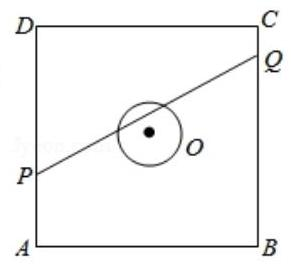
\includegraphics[max width=0.2\textwidth]{images/bo_d5jm9o77aajc7383vmi0_118_1159_1338_291_267_0.jpg}
\end{center}
\hspace*{3em} 

【例题】5. (2018 上海春考)如图，正方形角 \({ABCD}\) 的边长为20米，圆 \(O\) 的半径为1米，圆心是正方形的中心，点 \(P\) 、 \(Q\) 分别在线段 \({AD}\) 、 \({CB}\) 上，若线段 \({PQ}\) 与圆 \(O\) 有公共点,则称点 \(Q\) 在点 \(P\) 的“盲区”中,已知点 \(P\) 以 1.5 米/秒的速度从 \(A\) 出发向 \(D\) 移动. 同时,点 \(Q\) 以 1 米/秒的速度从 \(C\) 出发向 \(B\) 移动，则在点 \(P\) 从 \(A\) 移动到 \(D\) 的过程中，点 \(Q\) 在点 \(P\) 的盲区中的时长约为\_\_\_\_\_秒(精确到 0.1).

【答案】 4.4

【解析】以 \(O\) 为坐标原点,建立如图所示的直角坐标系,

\begin{center}
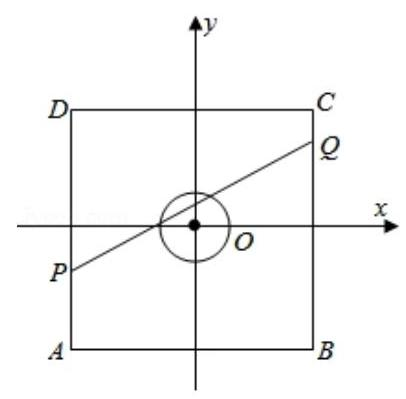
\includegraphics[max width=0.3\textwidth]{images/bo_d5jm9o77aajc7383vmi0_118_1048_1675_406_399_0.jpg}
\end{center}
\hspace*{3em} 

设 \(P\left( {-{10}, - {10} + {1.5t}}\right) ,Q\left( {{10},{10} - t}\right)\) ,

得直线 \({PQ}\) 的方程为 \(y - {10} + t = \frac{{20} - {2.5t}}{20}\left( {x - {10}}\right)\) ,圆 \(O\) 的方程为 \({x}^{2} + {y}^{2} = 1\) ,

由直线 \({PQ}\) 与圆 \(O\) 有交点,

得 \(\frac{\left| \frac{{2.5t} - {20}}{2} - t + {10}\right| }{\sqrt{1 + {\left( \frac{{20} - {2.5t}}{20}\right) }^{2}}} \leq  1\) ,

化为 \(3{t}^{2} + {16t} - {128} \leq  0\) ,解得 \(0 \leq  t \leq  \frac{8\sqrt{7} - 8}{3}\) ,

即有点 \(Q\) 在点 \(P\) 的盲区中的时长约为 4.4 秒. 2025 版上海高考真题及模拟训练合集(下册)

\section*{2. 模拟练习}

【练习】1. (2024 届交附) 椭圆具有如下的声学性质:从一个焦点出发的声波经过椭圆反射后会经过另外一个焦点. 有一个具有椭圆形光滑墙壁的建筑，某人站在一个焦点处大喊一声，声音向各个方向传播后经墙壁反射 (不考虑能量损失)，该人先后三次听到了回音，其中第一、二次的回音较弱，第三次的回音较强；记第一、二次听到回音的时间间隔为 \(x\) ，第二、三次听到回音的时间间隔为 \(y\) ,则椭圆的离心率为 ( )

A. \(\frac{x}{{2x} + y}\) B. \(\frac{x}{x + {2y}}\) C. \(\frac{y}{{2x} + y}\) D. \(\frac{y}{x + {2y}}\)

【答案】 \(B\)

【解析】情景还原, \({t}_{1}\) 时刻,刚刚呐喊声音传播为 \(0,{t}_{2}\) 时刻听到第一次回声,

声音的路程为 \(2\left( {a - c}\right)\) ，即从左交点到左顶点再次回到左焦点，

\({t}_{3}\) 时刻，声音的路程为 \(2\left( {a + c}\right)\) ，即从左焦点到右顶点，又从右顶点回到左点

\({t}_{4}\) 时刻，声音的路程为 \({4a}\) ，即由左焦点反射到右焦点，再反射到左焦点

所以有 \(x = {t}_{3} - {t}_{2}\) ,所以 \(2\left( {a + c}\right)  - 2\left( {a - c}\right)  = {vx}\) ,

所以有 \(y = {t}_{4} - {t}_{3}\) ,所以 \({4a} - 2\left( {a + c}\right)  = {vy}\) ,

接下来处理, \({4c} = {vx},{2a} - {2c} = {vy}\) ,所以 \(\frac{a - c}{2c} = \frac{y}{x}\) ,

所以 \(\frac{a - c}{c} = \frac{2y}{x}\) ,所以 \(\frac{a}{c} - 1 = \frac{2y}{x}\) ,所以 \(\frac{a}{c} = \frac{{2y} + x}{x}\) ,即 \(\frac{c}{a} = \frac{x}{{2y} + x}\) ,故选 \(B\)

【练习】2. (2024 届华二) 如图是一款电动自行车用“遮阳神器”的结构示意图，它由三叉形的支架 \(O - {ABC}\) 和覆盖在支架上的遮阳布 \(\bigtriangleup {ABC}\) 组成. 已知 \({OA} = {1.4}\) 米, \({OB} = {OC} = {0.6}\) 米,且 \(\angle {AOB} = \angle {AOC}\) . 为保障行车安全,要求遮阳布的最宽处 \({BC} \leq  1\) 米. 若希望遮阳效果最好 (即 \(\bigtriangleup {ABC}\) 的面积最大)，则 \(\angle {BOC}\) 的大小约为\_\_\_\_\_ (结果四舍五入精确到 \({1}^{ \circ  }\) ).

\begin{center}
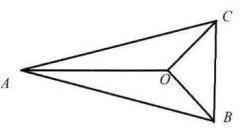
\includegraphics[max width=0.2\textwidth]{images/bo_d5jm9o77aajc7383vmi0_119_1225_1119_242_136_0.jpg}
\end{center}
\hspace*{3em} 

【答案】 \({113}^{ \circ  }\)

【解析】若 \(O\) 不在平面 \({ABC}\) 上,设 \(P\) 为 \(O\) 在平面 \({ABC}\) 上的射影.

在 \({PA}\text{ 、 }{PB}\text{ 、 }{PC}\) 的延长线上分别取点 \(D\text{ 、 }E\text{ 、 }F\) ,使得 \({PD} = {OA}\text{ 、 }{PE} = {OB}\) 、

\({PF} = {OC}\) ，此时， \({S}_{\bigtriangleup {DEF}} > {S}_{\bigtriangleup {ABC}}\) ，故当 \(\bigtriangleup  {ABC}\) 的面积最大时， \(O\) 必在平面 \({ABC}\) 上.

设 \(\angle {BOC} = {2\theta }\) ，则 \(2 \times  {0.6}\sin \theta  \leq  1\) ，即 \(0 < \theta  \leq  \arcsin \frac{5}{6}\) .

\({S}_{\bigtriangleup {ABC}} = \frac{1}{2}\left| {BC}\right| \left( {\left| {OA}\right|  + \left| {OC}\right| \cos \theta }\right)  = {0.6}\sin \theta \left( {{1.4} + {0.6}\cos \theta }\right)\) ,

设 \(f\left( \theta \right)  = {0.84}\sin \theta  + {0.18}\sin {2\theta }\) ,

则 \({f}^{\prime }\left( \theta \right)  = {0.84}\cos \theta  + {0.36}\cos {2\theta } = {0.12}\left( {3\cos \theta  - 1}\right) \left( {2\cos \theta  + 3}\right)\) ,

当 \(0 < \theta  \leq  \arcsin \frac{5}{6}\) 时, \(\cos \theta  \geq  \frac{\sqrt{11}}{6} > \frac{1}{3}\) ,故 \({f}^{\prime }\left( \theta \right)  > 0\) ,函数 \(y = f\left( \theta \right)\) 严格增,

因此 \(\bigtriangleup {ABC}\) 的面积最大时 \(\angle {BOC} = 2\arcsin \frac{5}{6} \approx  {113}^{ \circ  }\) .

【练习】3. (2024 上海三模) 舒腾尺是荷兰数学家舒腾 (1615-1660) 设计的一种作图工具，如图, \(O\) 是滑槽 \({AB}\) 的中点，短杆 \({ON}\) 可绕 \(O\) 转动，长杆 \({MN}\) 通过 \(N\) 处的铰链与 \({ON}\) 连接， \({MN}\) 上的栓子 \(D\) 可沿滑槽 \({AB}\) 滑动,当点 \(D\) 在滑槽 \({AB}\) 内作往复移动时,带动点 \(N\) 绕 \(O\) 转动,点 \(M\) 也随之而运动,记点 \(N\) 的运动轨迹为 \({C}_{1}\) ,点 \(M\) 的运动轨迹为 \({C}_{2}\) . 若 \({ON} = {DN} = 1,{MN} = 3\) ,且 \({AB} \geq  4\) ,过 \({C}_{2}\) 上的点 \(P\) 向 \({C}_{1}\) 作切线,则切线长的最大值为\_\_\_\_\_ 2025 版上海高考真题及模拟训练合集(下册)

\begin{center}
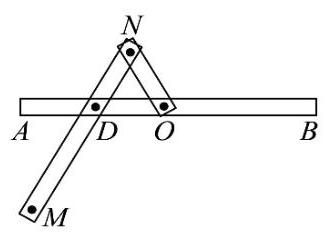
\includegraphics[max width=0.2\textwidth]{images/bo_d5jm9o77aajc7383vmi0_120_293_232_326_236_0.jpg}
\end{center}
\hspace*{3em} 

【答案】 \(\sqrt{15}\)

【解析】如图,以滑槽 \({AB}\) 所在的直线为 \(x\) 轴, \(O\) 为坐标原点建立平面直角坐标系,

因为 \({ON} = 1\) ,所以点 \(N\) 的运动轨迹 \({C}_{1}\) 是以 \(O\) 为圆心,1 为半径的圆,

\begin{center}
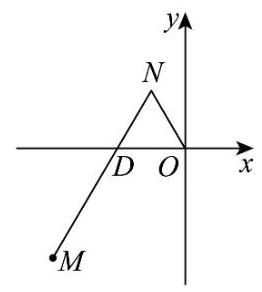
\includegraphics[max width=0.2\textwidth]{images/bo_d5jm9o77aajc7383vmi0_120_1194_618_262_292_0.jpg}
\end{center}
\hspace*{3em} 

则其方程为 \({x}^{2} + {y}^{2} = 1\) ,

设 \(N\left( {\cos \theta ,\sin \theta }\right)\) ,因为 \({ON} = {DN} = 1\) ,所以 \(D\left( {2\cos \theta ,0}\right)\) ,

因为 \({MN} = 3\) ，所以 \(\overrightarrow{NM} = 3\overrightarrow{ND}\) ，

设 \(M\left( {x,y}\right)\) ,则 \(\left( {x - \cos \theta ,y - \sin \theta }\right)  = 3\left( {\cos \theta , - \sin \theta }\right)\) ,得 \(x = 4\cos \theta ,y = \; - 2\sin \theta\) ,

所以 \(M\left( {4\cos \theta , - 2\sin \theta }\right)\) ,则点 \(M\) 的轨迹 \({C}_{2}\) 是椭圆,其方程为 \(\frac{{x}^{2}}{16} + \frac{{y}^{2}}{4} =\)

1,

设 \({C}_{2}\) 上的点 \(P\left( {4\cos \alpha , - 2\sin \alpha }\right)\) ,则

\(O{P}^{2} = {16}{\cos }^{2}\alpha  + 4{\sin }^{2}\alpha  = 4 + {12}{\cos }^{2}\alpha  \leq  {16}\) ,

所以切线长为 \(\sqrt{O{P}^{2} - 1} \leq  \sqrt{{16} - 1} = \sqrt{15}\) ,

所以切线长的最大值为 \(\sqrt{15}\) ,

故答案为: \(\sqrt{15}\)

【练习】4. (2024 届华二)如图所示，甲工厂位于一直线河岸的岸边 \(A\) 处，乙工厂与甲工厂在河的同侧， 且位于离河岸 \({40}\mathrm{\;{km}}\) 的 \(B\) 处，河岸边 \(D\) 处与 \(A\) 处相距 \({50}\mathrm{{km}}\) (其中 \({BD} \bot  {AD}\) )，两家工厂要在此岸边建一个供水站 \(C\) ,从供水站到甲工厂和乙工厂的水管费用分别为每千米 \({3a}\) 元和 \({5a}\) 元, 问供水站 \(C\) 建在岸边距离 \(A\) 处\_\_\_\_\_ \(\mathrm{{km}}\) 才能使水管费用最省？

\begin{center}
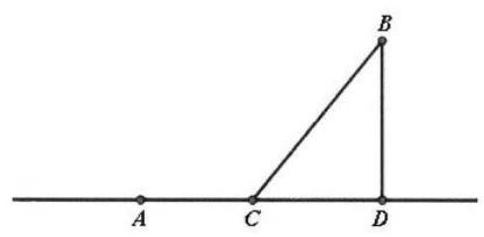
\includegraphics[max width=0.4\textwidth]{images/bo_d5jm9o77aajc7383vmi0_120_291_1396_484_237_0.jpg}
\end{center}
\hspace*{3em} 

【答案】 20

【解析】由题意得点 \(C\) 在线段 \({AD}\) 上才能使水管费用最省,

设 \(C\) 点距 \(D\) 点 \(x\mathrm{\;{km}}\) ,则 \({BD} = {40},{AC} = {50} - x,{BC} = \sqrt{B{D}^{2} + C{D}^{2}} = \sqrt{{x}^{2} + {40}^{2}}\) ;

设水管总费用为 \(y\) 元,由题意得 \(y = {3a}\left( {{50} - x}\right)  + {5a}\sqrt{{x}^{2} + {40}^{2}}\left( {0 < x < {50}}\right)\) .

其导数为 \({y}^{\prime } =  - {3a} + \frac{5ax}{\sqrt{{x}^{2} + {40}^{2}}}\) .

令 \({y}^{\prime } = 0\) ,解得函数的驻点为 \(x = {30}\) .

当 \(x \in  \left( {0,{30}}\right)\) 时, \({y}^{\prime } < 0\) ,函数在区间 \(\left( {0,{30}}\right)\) 上严格递减;

当 \(x \in  \left( {{30},{50}}\right)\) 时, \({y}^{\prime } > 0\) ,函数 \(V\left( x\right)\) 在区间 \(\left( {{30},{50}}\right)\) 上严格递增.

因此,在区间 \(\left( {0,{50}}\right)\) 上, \(y\) 只有一个极值点.

2025 版上海高考真题及模拟训练合集(下册)

根据实际问题的意义，函数在 \(x = {30}\left( \mathrm{\;{km}}\right)\) 处取得最小值，

此时 \({AC} = {50} - x = {20}\left( \mathrm{\;{km}}\right)\) .

所以,供水站建在 \(A\text{ 、 }D\) 之间距甲厂 \({20}\mathrm{\;{km}}\) 处,可使水管费用最省.

2025 版上海高考真题及模拟训练合集(下册)

【练习】5. (2024 届复附) 《周髀算经》中“侧影探日行”一文有记载:“即取竹空，径一寸，长八尺，捕影而视之，空正掩目，而日应空之孔.”意为“取竹空这一望筒，当望筒直 \(d\) 是一寸，筒长 \(t\) 是八尺时 (注:一尺等于十寸)，从筒中搜捕太阳的边缘观察，则筒的内孔正好覆盖太阳，而太阳的外缘恰好填满竹管的内孔.”如图所示， \(O\) 为竹空底面圆心，则太阳角 \(\angle {AOB}\) 的正切值为( )

\begin{center}
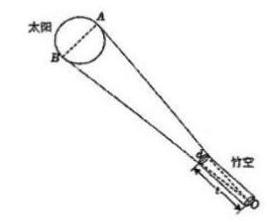
\includegraphics[max width=0.2\textwidth]{images/bo_d5jm9o77aajc7383vmi0_122_298_427_267_222_0.jpg}
\end{center}
\hspace*{3em} 

A. \(\frac{1}{160}\) B. \(\frac{320}{{160}^{2} - 1}\) C. \(\frac{1}{80}\) D. \(\frac{160}{{80}^{2} - 1}\)

【答案】 \(B\)

【解析】由题意得 \(\frac{d}{t} = \frac{1}{80},\tan \frac{\angle {AOB}}{2} = \frac{\frac{d}{2}}{t} = \frac{d}{2t} = \frac{1}{160}\) , 由二倍角的正切公式得 \(\tan \angle {AOB} = \frac{2\tan \frac{\angle {AOB}}{2}}{1 - {\tan }^{2}\frac{\angle {AOB}}{2}} = \frac{2 \times  \frac{1}{160}}{1 - {\left( \frac{1}{160}\right) }^{2}} = \frac{320}{{160}^{2} - 1}\) 故选 \(B\)

\begin{center}
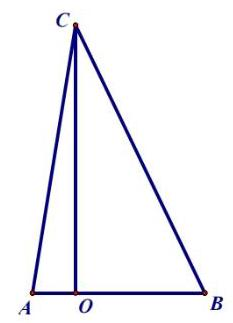
\includegraphics[max width=0.2\textwidth]{images/bo_d5jm9o77aajc7383vmi0_122_1206_1095_233_323_0.jpg}
\end{center}
\hspace*{3em} 

【练习】6. (2025 届格致) 如图,已知点 \(C\) 在点 \(O\) 的正北方向,点 \(A\) 、点 \(B\) 分别在点 \(O\) 的正西、正东方向,且 \(\sin \angle {ACB} = \frac{4}{7},\sin \left( {A - B}\right)  = \frac{2}{7},{AB} = 4\) ,若 \(\angle {ACB}\) 为锐角,则 \({OC} =\) \_\_\_\_\_.

【答案】 \(\frac{\sqrt{33} + 3\sqrt{5}}{2}\)

【解析】由 \(\sin \angle {ACB} = \sin \left( {A + B}\right)  = \frac{4}{7},\sin \left( {A - B}\right)  = \frac{2}{7}\) ,

得 \(\sin A\cos B = \frac{3}{7},\cos A\sin B = \frac{1}{7}\) ，所以 \(\frac{\tan A}{\tan B} = 3\) ，则 \(\frac{OB}{OA} = 3\) ，

又 \({AB} = 4\) ，所以 \({OA} = 1,{OB} = 3\) ，

所以 \(\sin A = \frac{OC}{\sqrt{1 + O{C}^{2}}},\cos B = \frac{3}{\sqrt{9 + O{C}^{2}}}\) ，则 \(\frac{OC}{\sqrt{1 + O{C}^{2}}} \cdot  \frac{3}{\sqrt{9 + O{C}^{2}}} = \frac{3}{7}\) ，

解得 \({OC} = \frac{\sqrt{33} + 3\sqrt{5}}{2}\) .

2025 版上海高考真题及模拟训练合集(下册)

【练习】7. (2024 届上中)为解决皮尺长度不够的问题，实验小组利用自行车来测量 \(A\) 、 \(B\) 两点之间的直线距离. 如图，先将自行车前轮置于点 \(A\) ，前轮上与点 \(A\) 接触的地方标记为点 \(C\) ，然后推着自行车沿 \({AB}\) 直线前进 (车身始终保持与地面垂直),直到前轮与点 \(B\) 接触. 经观测,在前进过程中，前轮上的标记点 \(C\) 与地面接触了 10 次，当前轮与点 \(B\) 接触时，标记点 \(C\) 在前轮的左上方 (以如图为观察视角),且到地面的垂直高度为 \({0.45}\mathrm{\;m}\) . 已知前轮的半径为 \({0.3}\mathrm{\;m}\) ,则 \(A\text{ 、 }B\) 两点之间的距离约为\_\_\_\_\_(计算结果精确到小数点后第二位).

\begin{center}
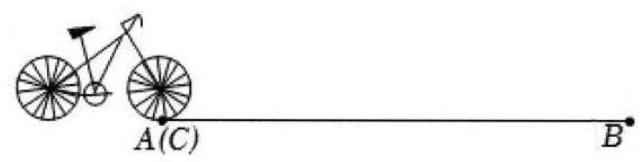
\includegraphics[max width=0.5\textwidth]{images/bo_d5jm9o77aajc7383vmi0_123_293_511_641_162_0.jpg}
\end{center}
\hspace*{3em} 

【答案】 19.47 \(m\)

【解析】由题意得,前轮转动了 \(\left( {{10} + \frac{1}{3}}\right)\) 圈,

故 \(A\text{ 、 }B\) 两点之间的距离约为 \(\left( {{10} + \frac{1}{3}}\right)  \times  {2\pi } \times  {0.3} = {6.2\pi } \approx  {19.47}\mathrm{\;m}\) .

【练习】8. (2025 届交附) 在一座尖塔的正南方向地面某点 \(A\) ,测得塔顶的仰角为 \({30}^{ \circ  }\) ,又在此尖塔北偏东 \({30}^{ \circ  }\) 地面某点 \(B\) ,测得塔顶的仰角为 \({45}^{ \circ  }\) ,且 \(A\text{ 、 }B\) 两点距离为 \(7\mathrm{\;m}\) ,在线段 \({AB}\) 上的点 \(C\) 处测得塔顶的仰角为最大，则 \(C\) 点到塔底 \(O\) 的距离为\_\_\_\_\_ \(m\)

【答案】 \(\frac{\sqrt{3}}{2}\)

【解析】设尖塔高为 \({OP}\) ,设 \({OP} = m\) ,

由题意得 \(\angle {AOB} = {150}^{ \circ  },\angle {PAO} = {30}^{ \circ  },\angle {PBO} = {45}^{ \circ  }\) ,

\begin{center}
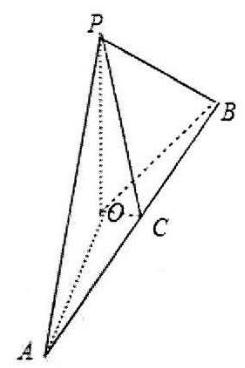
\includegraphics[max width=0.2\textwidth]{images/bo_d5jm9o77aajc7383vmi0_123_1215_1162_245_368_0.jpg}
\end{center}
\hspace*{3em} 

所以 \({OA} = \sqrt{3}m,{OB} = m\) ,

在 \(\bigtriangleup  {AOB}\) 中，由余弦定理得 \(A{B}^{2} = O{A}^{2} + O{B}^{2} - {2OA} \cdot  {OB} \cdot  \cos \angle {AOB}\) ，

所以 \({49} = 3{m}^{2} + {m}^{2} - 2\sqrt{3}m \cdot  m \cdot  \left( {-\frac{\sqrt{3}}{2}}\right)  = 7{m}^{2}\) ,

所以 \(m = \sqrt{7}\) ,所以 \({OA} = \sqrt{21},{OB} = \sqrt{7}\) ,

在线段 \({AB}\) 上的点 \(C\) 处测得塔顶的仰角为最大,则 \(C\) 到 \(O\) 的距离最小, 即 \({OC}\) 为 \(O\) 到 \({AB}\) 的距离,

作 \({OC} \bot  {AB},C\) 为垂足,则 \({OC}\) 为所求

由 \({S}_{\bigtriangleup {ABO}} = \frac{1}{2} \times  {OA} \times  {OB} \times  \sin {150}^{ \circ  } = \frac{1}{2} \times  {OC} \times  {AB}\) ,

得 \(\frac{1}{2} \times  \sqrt{21} \times  \sqrt{7} \times  \frac{1}{2} = \frac{1}{2} \times  7 \times  {OC}\) ,解得 \({OC} = \frac{\sqrt{3}}{2}\)

\section*{板块二: 基础主观题}

\section*{1. 真题回顾}

【例题】1. (2020 上海秋考) 在研究某市交通情况时, 道路密度是指该路段上一定时间内通过的车辆数除以时间，车辆密度是该路段一定时间内通过的车辆数除以该路段的长度，

现定义交通流量为 \(v = \frac{q}{x},x\) 为道路密度， \(q\) 为车辆密度，

交通流量 \(v = f\left( x\right)  = \left\{  \begin{array}{ll} {100} - {135} \cdot  {\left( \frac{1}{3}\right) }^{\frac{80}{x}}, & 0 < x < {40} \\   - k\left( {x - {40}}\right)  + {85}, & {40} \leq  x \leq  {80} \end{array}\right.\) , \(k > 0\) .

(1)若交通流量 \(v > {95}\) ，求道路密度 \(x\) 的取值范围；

(2)已知道路密度 \(x = {80}\) 时，测得交通流量 \(v = {50}\) ，求车辆密度 \(q\) 的最大值.

【解析】(1) 因为 \(v = \frac{q}{x}\) ,所以 \(v\) 越大， \(x\) 越小，

所以 \(v = f\left( x\right)\) 是单调递减函数, \(k > 0\) ,

当 \({40} \leq  x \leq  {80}\) 时, \(v\) 最大为 85,

于是只需令 \({100} - {135} \cdot  {\left( \frac{1}{3}\right) }^{\frac{80}{x}} > {95}\) ,解得 \(x < \frac{80}{3}\) ,

故道路密度 \(x\) 的取值范围为 \(\left( {0,\frac{80}{3}}\right)\) .

(2)把 \(x = {80},v = {50}\) 代入 \(v = f\left( x\right)  =  - k\left( {x - {40}}\right)  + {85}\) 中，

得 \({50} =  - k \cdot  {40} + {85}\) ,解得 \(k = \frac{7}{8}\) .

所以 \(q = {vx} = \left\{  \begin{array}{ll} {100x} - {135} \cdot  {\left( \frac{1}{3}\right) }^{\frac{80}{x}} \cdot  x, & 0 < x < {40} \\   - \frac{7}{8}\left( {x - {40}}\right) x + {85x}, & {40} \leq  x \leq  {80} \end{array}\right.\) ,

 \circled{1}  当 \(0 < x < {40}\) 时, \(v = {100} - {135} \cdot  {\left( \frac{1}{3}\right) }^{\frac{80}{x}} < {100},q = {vx} < {100} \times  {40} = {4000}\) .

 \circled{2}  当 \({40} \leq  x \leq  {80}\) 时， \(q\) 是关于 \(x\) 的二次函数， \(q =  - \frac{7}{8}{x}^{2} + {120x}\) ，

对称轴为 \(x = \frac{480}{7}\) ，此时 \(q\) 有最大值，

为 \(- \frac{7}{8} \times  {\left( \frac{480}{7}\right) }^{2} + {120} \times  \frac{480}{7} = \frac{28800}{7} > {4000}\) .

综上所述，车辆密度 \(q\) 的最大值为 \(\frac{28800}{7}\) .

【例题】2. (2019 上海春考) 改革开放 40 年，我国卫生事业取得巨大成就，卫生总费用增长了数十倍. 卫生总费用包括个人现在支出、社会支出、政府支出，如表为 2012 年 -2015 年我国卫生费用中个人现金支出、社会支出和政府支出的费用 (单位:亿元) 和在卫生总费用中的占比. 2025 版上海高考真题及模拟训练合集(下册)

\begin{center}
\adjustbox{max width=\textwidth}{
\begin{tabular}{|c|c|c|c|c|c|c|c|}
\hline
\multirow{2}{*}{年份} & \multirow{2}{*}{卫生总费用 (亿元)} & \multicolumn{2}{|c|}{个人现金卫生支出} & \multicolumn{2}{|c|}{社会卫生支出} & \multicolumn{2}{|c|}{政府卫生支出} \\
\cline{3-8}
 &  & 绝对数 (亿元) & 占卫生总费用比重 (\%) & 绝对数 (亿元) & 占卫生总费用比重 (\%) & 绝对数 (亿元) & 占卫生总费用比重 (\%) \\
\cline{1-8}
2012 & 28119.0 0 & 9656.32 & 34.34 & 10030.70 & 35.67 & 8431.98 & 29.99 \\
\cline{1-8}
\hline
\end{tabular}
}
\end{center}

\begin{center}
\adjustbox{max width=\textwidth}{
\begin{tabular}{|c|c|c|c|c|c|c|c|}
\hline
2013 & 31668.9 5 & 10729.34 & 33.88 & 11393.79 & 35.98 & 9545.81 & 30.14 \\
\cline{1-8}
2014 & 35312.4 0 & 11295.41 & 31.99 & 13437.75 & 38.05 & 10579.2 3 & 29.96 \\
\cline{1-8}
2015 & 40974.6 4 & 11992.65 & 29.27 & 16506.71 & 40.29 & 12475.2 8 & 30.45 \\
\cline{1-8}
\hline
\end{tabular}
}
\end{center}

(数据来源于国家统计年鉴)

(1)指出 2012 年到 2015 年之间我国卫生总费用中个人现金支出占比和社会支出占比的变化趋势:

(2)设 \(t = 1\) 表示1978 年，第 \(n\) 年卫生总费用与年份 \(t\) 之间拟合函数 \(f\left( t\right)  = \frac{357876.6053}{1 + {\mathrm{e}}^{{6.4420} - {0.1136t}}}\) 研究函数 \(f\left( t\right)\) 的单调性，并预测我国卫生总费用首次超过 12 万亿的年份.

【解析】(1) 由表格数据得个人现金支出占比逐渐减少, 社会支出占比逐渐增多.

(2) 因为 \(y = {\mathrm{e}}^{{6.4420} - {0.1136t}}\) 是减函数,且 \(y = {\mathrm{e}}^{{6.4420} - {0.1136t}} > 0\) ,

所以 \(f\left( t\right)  = \frac{357876.6053}{1 + {\mathrm{e}}^{{6.4420} - {0.1136t}}}\) 在 \(N\) 上单调递增,

令 \(\frac{357876.6053}{1 + {\mathrm{e}}^{{6.4420} - {0.1136t}}} > {120000}\) ,解得 \(t > {50.68}\) ,

所以当 \(t \geq  {51}\) 时,我国卫生总费用超过 12 万亿,

所以预测我国到 2028 年我国卫生总费用首次超过 12 万亿.

【例题】3. (2018 上海秋考) 某群体的人均通勤时间, 是指单日内该群体中成员从居住地到工作地的平均用时. 某地上班族 \(S\) 中的成员仅以自驾或公交方式通勤. 分析显示: 当 \(S\) 中 \(x\% (0 < x <\) 100) 的成员自驾时,自驾群体的人均通勤时间为 \(f\left( x\right)  = \left\{  \begin{array}{ll} {30}, & 0 < x \leq  {30} \\  {2x} + \frac{1800}{x} - {90}, & {30} < x < {100} \end{array}\right.\) (单位:分钟)，而公交群体的人均通勤时间不受 \(x\) 影响，恒为 40 分钟，试根据上述分析结果回答下列问题:

(1)当 \(x\) 在什么范围内时,公交群体的人均通勤时间少于自驾群体的人均通勤时间？

(2)求该地上班族 \(S\) 的人均通勤时间 \(g\left( x\right)\) 的表达式；讨论 \(g\left( x\right)\) 的单调性，并说明其实际意义.

【解析】(1) 由题意得当 \({30} < x < {100}\) 时, \(f\left( x\right)  = {2x} + \frac{1800}{x} - {90} > {40}\) ,

即 \({x}^{2} - {65x} + {900} > 0\) ,解得 \(x < {20}\) 或 \(x > {45}\) ,

所以 \(x \in  \left( {{45},{100}}\right)\) 时,公交群体的人均通勤时间少于自驾群体的人均通勤时间;

(2) 当 \(0 < x \leq  {30}\) 时, \(g\left( x\right)  = {30} \cdot  x\%  + {40}\left( {1 - x\% }\right)  = {40} - \frac{x}{10}\) ;

当 \({30} < x < {100}\) 时, \(g\left( x\right)  = \left( {{2x} + \frac{1800}{x} - {90}}\right)  \cdot  x\%  + {40}\left( {1 - x\% }\right)\)

\(= \frac{{x}^{2}}{50} - \frac{13}{10}x + {58}\)

所以 \(g\left( x\right)  = \left\{  \begin{array}{l} {40} - \frac{x}{10} \\  \frac{{x}^{2}}{50} - \frac{13}{10}x + {58} \end{array}\right.\) ;

当 \(0 < x < {32.5}\) 时, \(g\left( x\right)\) 单调递减; 当 \({32.5} < x < {100}\) 时, \(g\left( x\right)\) 单调递增;

说明该地上班族 \(S\) 中有小于 32.5\% 的人自驾时，人均通勤时间是递减的；

有大于 32.5\% 的人自驾时，人均通勤时间是递增的；

当自驾人数所占比为 32.5\% 时,人均通勤时间最少.

【例题】4. (2017 上海秋考) 根据预测,某地第 \(n\left( {n \in  {N}^{ * }}\right)\) 个月共享单车的投放量和损失量分别为 \({a}_{n}\) 和 \({b}_{n}\) (单位: 辆),其中 \({a}_{n} = \left\{  {\begin{array}{ll} 5{n}^{4} + {15}, & 1 \leq  n \leq  3 \\   - {10n} + {470}, & n \geq  4 \end{array},{b}_{n} = n + 5}\right.\) ,第 \(n\) 个月底的共享单车的保有量是前 \(n\) 个月的累计投放量与累计损失量的差.

(1)求该地区第 4 个月底的共享单车的保有量；

(2)已知该地共享单车停放点第 \(n\) 个月底的单车容纳量 \({S}_{n} =  - 4{\left( n - {46}\right) }^{2} + {8800}\) (单位:辆). 设在某月底, 共享单车保有量达到最大, 问该保有量是否超出了此时停放点的单车容纳量?

【解析】(1) 因为 \({a}_{n} = \left\{  {\begin{array}{ll} 5{n}^{4} + {15}, & 1 \leq  n \leq  3 \\   - {10n} + {470}, & n \geq  4 \end{array},{b}_{n} = n + 5}\right.\) ,所以 \({a}_{1} = 5 \times  {1}^{4} + {15} = {20}\) ,

\({a}_{2} = 5 \times  {2}^{4} + {15} = {95},{a}_{3} = 5 \times  {3}^{4} + {15} = {420},{a}_{4} =  - {10} \times  4 + {470} = {430}\) ,

\({b}_{1} = 1 + 5 = 6,{b}_{2} = 2 + 5 = 7,{b}_{3} = 3 + 5 = 8,{b}_{4} = 4 + 5 = 9\) ,

所以前 4 个月共投放单车为 \({a}_{1} + {a}_{2} + {a}_{3} + {a}_{4} = {20} + {95} + {420} + {430} = {965}\) ,

前 4 个月共损失单车为 \({b}_{1} + {b}_{2} + {b}_{3} + {b}_{4} = 6 + 7 + 8 + 9 = {30}\) ,

所以该地区第 4 个月底的共享单车的保有量为 \({965} - {30} = {935}\) .

(2)令 \({a}_{n} \geq  {b}_{n}\) ，显然， \(n \leq  3\) 时恒成立，

当 \(n \geq  4\) 时，有 \(- {10n} + {470} \geq  n + 5\) ，解得 \(n \leq  \frac{465}{11}\) ，

所以第 42 个月底, 保有量达到最大.

当 \(n \geq  4,\left\{  {a}_{n}\right\}\) 为公差为 -10 的等差数列,而 \(\left\{  {b}_{n}\right\}\) 为等差为 1 的等差数列,

所以到第 42 个月底,单车保有量为 \(\frac{{a}_{4} + {a}_{42}}{2} \times  {39} + {935} - \frac{{b}_{1} + {b}_{42}}{2} \times  {42}\)

\(= \frac{{430} + {50}}{2} \times  {39} + {935} - \frac{6 + {47}}{2} \times  {42} = {8782}.\)

\({S}_{42} =  - 4 \times  {16} + {8800} = {8736}.\)

因为 \({8782} > {8736}\) ,所以第 42 个月底单车保有量超过了容纳量.

\begin{center}
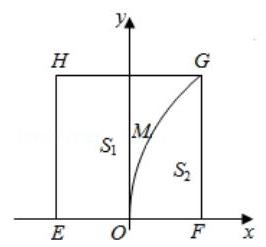
\includegraphics[max width=0.2\textwidth]{images/bo_d5jm9o77aajc7383vmi0_126_1179_1456_266_247_0.jpg}
\end{center}
\hspace*{3em} 

【例题】5. (2016上海秋考)有一块正方形 \({EFGH}\) ， \({EH}\) 所在直线是一条小河，收获的蔬菜可送到 \(F\) 点或河边运走. 于是,菜地分别为两个区域 \({S}_{1}\) 和 \({S}_{2}\) , 其中 \({S}_{1}\) 中的蔬菜运到河边较近, \({S}_{2}\) 中的蔬菜运到 \(F\) 点较近,而菜地内 \({S}_{1}\) 和 \({S}_{2}\) 的分界线 \(C\) 上的点到河边与到 \(F\) 点的距离相等,现建立平面直角坐标系,其中原点 \(O\) 为 \({EF}\) 的中点,点 \(F\) 的坐标为 \(\left( {1,0}\right)\) ,如图.

(1)求菜地内的分界线 \(C\) 的方程；

(2)菜农从蔬菜运量估计出 \({S}_{1}\) 面积是 \({S}_{2}\) 面积的两倍，由此得到 \({S}_{1}\) 面积的经验值为 \(\frac{8}{3}\) . 设 \(M\) 是 \(C\) 上纵坐标为 1 的点,请计算以 \({EH}\) 为一边,另一边过点 \(M\) 的矩形的面积,及五边形 EOMGH 的面积,并判断哪一个更接近于 \({S}_{1}\) 面积的“经验值”.

\begin{center}
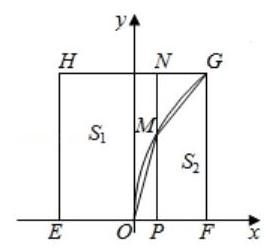
\includegraphics[max width=0.2\textwidth]{images/bo_d5jm9o77aajc7383vmi0_126_1187_1859_267_250_0.jpg}
\end{center}
\hspace*{3em} 

【解析】(1) 设分界线上任意一点为 \(\left( {x,y}\right)\) ,由题意得 \(\left| {x + 1}\right|  = \sqrt{{\left( x - 1\right) }^{2} + {y}^{2}}\) , 得 \(y = 2\sqrt{x}\left( {0 \leq  x \leq  1}\right)\) ,

(2)设 \(M\left( {{x}_{0},{y}_{0}}\right)\) ，则 \({y}_{0} = 1\) ，所以 \({x}_{0} = \frac{{y}_{0}^{2}}{4} = \frac{1}{4}\) ，

设所表述的矩形面积为 \({S}_{3}\) ,则 \({S}_{3} = 2 \times  \left( {\frac{1}{4} + 1}\right)  = 2 \times  \frac{5}{4} = \frac{5}{2}\) ,

设五边形 \({EMOGH}\) 的面积为 \({S}_{4}\) ,

则 \({S}_{4} = {S}_{3} - {S}_{\bigtriangleup {OMP}} + {S}_{\bigtriangleup {MGN}} = \frac{5}{2} - \frac{1}{2} \times  \frac{1}{4} \times  1 + \frac{1}{2} \times  \frac{3}{4} \times  1 = \frac{11}{4}\) ,

\({S}_{1} - {S}_{3} = \frac{8}{3} - \frac{5}{2} = \frac{1}{6},{S}_{4} - {S}_{1} = \frac{11}{4} - \frac{8}{3} = \frac{1}{12} < \frac{1}{6},\)

所以五边形 \({EMOGH}\) 的面积更接近 \({S}_{1}\) 的面积. 2025 版上海高考真题及模拟训练合集(下册)

\section*{2. 模拟练习}

【练习】1. (2023 届上中) 某地打算修建一条公路，但设计路线正好经过一个野生动物迁徙路线，为了保护野生动物, 决定修建高架桥, 为野生动物的迁徙提供安全通道. 若高架桥的两端及两端的桥墩已建好，两端的桥墩相距 1200 米，余下的工程只需要建两端桥墩之间的桥面和桥墩. 经预测，一个桥墩的工程费用为 500 万元，距离为 \(x\) 米的相邻两桥墩之间的桥面工程费用为 \({10x}\left\lbrack  {\ln \left( {x + {12}}\right)  - 3}\right\rbrack\) 万元. 假设桥墩等距离分布,所有桥墩都视为点,且不考虑其它因素,记余下工程的费用为 \(y\) 万元.

(1)试写出 \(y\) 关于 \(x\) 的函数关系式;

(2)需新建多少个桥墩才能使 \(y\) 最小?

【解析】(1) 需新建桥墩 \(\left( {\frac{1200}{x} - 1}\right)\) 个,

所以 \(y = {500}\left( {\frac{1200}{x} - 1}\right)  + \frac{1200}{x} \times  {10x}\left\lbrack  {\ln \left( {x + {12}}\right)  - 3}\right\rbrack\)

\(= \frac{600000}{x} - {500} + {12000}\ln \left( {x + {12}}\right)  - {36000}\)

\(= {12000}\left\lbrack  {\frac{50}{x} + \ln \left( {x + {12}}\right) }\right\rbrack   - {36500},x \in  \left( {0,{1200}}\right) ;\)

(2) 令 \(f\left( x\right)  = \frac{50}{x} + \ln \left( {x + {12}}\right) ,x \in  (0,{1200}\rbrack\) ,

\({f}^{\prime }\left( x\right)  =  - \frac{50}{{x}^{2}} + \frac{1}{x + {12}} = \frac{{x}^{2} - {50x} - {600}}{{x}^{2}\left( {x + {12}}\right) },\)

令 \({f}^{\prime }\left( x\right)  = 0\) ,解得 \(x = {60}\) 或 \(x =  - {10}\) (舍去),

当 \(x \in  \left( {0,{60}}\right)\) 时, \({f}^{\prime }\left( x\right)  < 0\) ,函数 \(f\left( x\right)\) 严格减,

当 \(x \in  ({60},{1200}\rbrack\) 时, \({f}^{\prime }\left( x\right)  > 0\) ,函数 \(f\left( x\right)\) 严格增,

所以 \(f{\left( x\right) }_{\min } = f\left( {60}\right)\) ,此时需新建 \(\left( {\frac{1200}{60} - 1}\right)  = {19}\) 个桥墩,

所以需新建 19 个桥墩才能使 \(y\) 最小.

【练习】2. (2024 届上中) 某商场在促销期间规定:商场内所有商品按标价的 80\% 出售，同时，当顾客在该商场内消费满一定金额后, 按如下方案获得相应金额的奖券:

\begin{center}
\adjustbox{max width=\textwidth}{
\begin{tabular}{|c|c|c|c|c|c|}
\hline
消费金额 (元)的范围 & [200, 400) & [400, 500) & [500, 700) & [700, 900) & ... \\
\cline{1-6}
获得奖券的金额(元) & 30 & 60 & 100 & 130 & ... \\
\cline{1-6}
\hline
\end{tabular}
}
\end{center}

根据上述促销方法, 顾客在该商场购物可以获得双重优惠, 例如, 购买标价为 400 元的商品, 则消费金额为 320 元,获得的优惠额为: \({400} \times  {0.2} + {30} = {110}\) (元),设购买商品得到的优惠率 \(= \frac{\text{ 购买商品获得的优惠额 }}{\text{ 商品的标价 }}\) ，试问:

(1)若购买一件标价为 1000 元的商品，顾客得到的优惠率是多少?

(2)对于标价在 \(\left\lbrack  {{500},{800}}\right\rbrack\) (元)内的商品，顾客购买标价为多少元的商品，可得到不小于 \(\frac{1}{3}\) 的优惠率?

【解析】(1) 由题意得 \(\frac{{1000} \times  {0.2} + {130}}{1000} = {33}\%\) .

故购买一件标价为 1000 元的商品, 顾客得到的优惠率是 33\%. 2025 版上海高考真题及模拟训练合集(下册)

(2)设商品的标价为 \(x\) 元.

则 \({500} \leq  x \leq  {800}\) ,消费额 \({400} \leq  {0.8x} \leq  {640}\) .

由题意得 \(\left( I\right) \left\{  \begin{array}{l} \frac{{0.2x} + {60}}{x} \geq  \frac{1}{3} \\  {400} \leq  {0.8x} \leq  {500} \end{array}\right.\) 或 \(\left( {II}\right) \left\{  \begin{array}{l} \frac{{0.2x} + {100}}{x} \geq  \frac{1}{3} \\  {500} \leq  {0.8x} \leq  {64} \end{array}\right.\)

不等式组 \(\left( I\right)\) 无解,不等式组 \(\left( {II}\right)\) 的解为 \({625} \leq  x \leq  {750}\) .

因此，当顾客购买标价在 \(\left\lbrack  {{625},{750}}\right\rbrack\) 元内的商品时，可得到不小于 \(\frac{1}{3}\) 的优惠率.

【练习】3. 某个体户计划经销 \(A\text{ 、 }B\) 两种商品,据调查统计,当投资额为 \(x\left( {x \geq  0}\right)\) 万元时,在经销 \(A\text{ 、 }B\) 商品中所获得的收益分别为 \(f\left( x\right)\) 万元与 \(g\left( x\right)\) 万元、其中 \(f\left( x\right)  = a\left( {x - 1}\right)  + 2\left( {a > 0}\right) ;g\left( x\right)  = \; 6\ln \left( {x + b}\right) \left( {b > 0}\right)\) . 已知投资额为零时,收益为零.

(1)试求出 \(a\text{ 、 }b\) 的值；

(2)如果该个体户准备投入 5 万元经营这两种商品，请你帮他制定一个资金投入方案，使他能获得最大收益, 并求出其收入的最大值 (精确到 0.1 万元).

【解析】(1) 由问题的实际意义,得 \(f\left( 0\right)  = 0,g\left( 0\right)  = 0\) ,即 \(\left\{  \begin{array}{l}  - a + 2 = 0 \\  6\ln b = 0 \end{array}\right.\) ,所以 \(\left\{  \begin{array}{l} a = 2 \\  b = 1 \end{array}\right.\) ;

(2) 由 (1) 得 \(f\left( x\right)  = {2x},g\left( x\right)  = 6\ln \left( {x + 1}\right)\) ，

设投入 \(B\) 商品的资金为 \(x\) 万元 \(\left( {0 \leq  x \leq  5}\right)\) ，则投入 \(A\) 商品的资金为 \(5 - x\) 万元，

若所获得的收入为 \(s\left( x\right)\) 万元，

则有 \(s\left( x\right)  = 2\left( {5 - x}\right)  + 6\ln \left( {x + 1}\right)  = 6\ln \left( {x + 1}\right)  - {2x} + {10}\left( {0 \leq  x \leq  5}\right)\) ,

所以 \({s}^{\prime }\left( x\right)  = \frac{6}{x + 1} - 2\) ,令 \({s}^{\prime }\left( x\right)  = 0\) ,得 \(x = 2\) ;

当 \(0 \leq  x < 2\) 时, \({s}^{\prime }\left( x\right)  > 0\) ; 当 \(2 < x \leq  5\) 时, \({s}^{\prime }\left( x\right)  < 0\) ,

所以 \(x = 2\) 是 \(s\left( x\right)\) 在区间 \(\left\lbrack  {0,5}\right\rbrack\) 上的唯一极大值点,此时 \(s\left( x\right)\) 取得最大值:

\(s{\left( x\right) }_{\max } = s\left( 2\right)  = 6\ln 3 + 6 \approx  {12.6}\) (万元),此时 \(5 - x = 3\) (万元)

答: 该个体户可对 \(A\) 商品投入 3 万元,对 \(B\) 商品投入 2 万元,

这样可以获得 12.6 万元的最大收益.

【练习】4. (2025 届交附) 某矿物质有 \(A\text{ 、 }B\) 两种冶炼方法,若使用 \(A\) 方法,所需费用 (单位:千元) 与矿物质的重量 (单位:吨) 的平方成正比，若使用 \(B\) 方法，所需费用 (单位:千元) 与矿物质的重量 (单位: 吨) 成正比,已知用 \(A\) 方法冶炼 2 吨、用 \(B\) 方法冶炼 1 吨所需的总费用为 14 千元,用 \(A\) 方法冶炼 1 吨、用 \(B\) 方法冶炼 2 吨所需的总费用也是 14 千元，现有该矿物质共 \(m\) 吨 \(\left( {m > 0}\right)\) ， 计划用 \(A\) 方法冶炼 \(x\) 吨 \(\left( {0 \leq  x \leq  m}\right)\) ，剩余部分用 \(B\) 方法冶炼，所需总费用为 \(y\) 千元

(1)建立 \(y\) 与 \(x\) 的函数关系:

(2)求总费用 \(y\) 的最小值，并说明其实际意义

【解析】(1) 设 \({y}_{A} = {k}_{1}{x}_{A}^{2},{y}_{B} = {k}_{2}{x}_{B}\) ,由题意得 \(\left\{  {\begin{array}{l} 4{k}_{1} + {k}_{2} = {14} \\  {k}_{1} + 2{k}_{2} = {14} \end{array} \Rightarrow  \left\{  \begin{array}{l} {k}_{1} = 2 \\  {k}_{2} = 6 \end{array}\right. }\right.\) ,

所需总费用 \(y = {y}_{A} + {y}_{B} = 2{x}_{A}^{2} + 6{x}_{B} = 2{x}^{2} + 6\left( {m - x}\right)\) ,且 \(x \in  \left\lbrack  {0,m}\right\rbrack\) ;

(2) 由 (1) 得 \(y = 2\left( {{x}^{2} - {3x}}\right)  + {6m} = 2{\left( x - \frac{3}{2}\right) }^{2} + {6m} - \frac{9}{2},x \in  \left\lbrack  {0,m}\right\rbrack\) ,

当 \(0 < m \leq  \frac{3}{2}\) 时, \(x = m\) 时总费用 \(y\) 的最小值,即全部用方法 \(A\) 冶炼费用最小;

当 \(m > \frac{3}{2}\) 时, \(x = \frac{3}{2}\) 时总费用 \(y\) 的最小值,即 1.5 吨用方法 \(A\) ,

剩余的用方法 \(B\) ,费用最小

【练习】5. (2025 届交附) 我国某西部地区进行沙漠治理，该地区有土地面积为 1 万平方千米，其中 70\% 的面积是沙漠，从今年起，该地区进行绿化改造，每年把上一年沙漠面积的 16\% 改造为绿洲,同时上一年绿洲面积的 4\% 被沙漠所侵蚀又变成沙漠. 设从今年起第 \(n\) 年绿洲面积为 \({a}_{n}\) 万平方千米

(1)求第 \(n\) 年绿洲面积 \({a}_{n}\) 与上一年绿洲面积 \({a}_{n - 1}\left( {n \geq  2}\right)\) 的关系;

( 2 )至少经过几年，绿洲面积可超过 60\%？

【解析】(1) 由题意得 \({a}_{n} = \left( {1 - 4\% }\right) {a}_{n - 1} + \left( {1 - {a}_{n - 1}}\right)  \times  {16}\%  = 0\) ,

\({96}{a}_{n - 1} + {0.16} - {0.16}{a}_{n - 1} = {0.8}{a}_{n - 1} + {0.16} = \frac{4}{5}{a}_{n - 1} + \frac{4}{25}\) ,

所以 \({a}_{n} = \frac{4}{5}{a}_{n - 1} + \frac{4}{25}\)

(2) 由 (1) 得 \({a}_{n} = \frac{4}{5}{a}_{n - 1} + \frac{4}{25}\) ,所以 \({a}_{n} - \frac{4}{5} = \frac{4}{5}\left( {{a}_{n - 1} - \frac{4}{5}}\right)\) ,

所以 \(\left\{  {{a}_{n} - \frac{4}{5}}\right\}\) 是等比数列,则 \({a}_{n} - \frac{4}{5} = \frac{4}{5}\left( {{a}_{n - 1} - \frac{4}{5}}\right)\) ,

又 \({a}_{1} = \frac{3}{10}\) ，所以 \({a}_{1} - \frac{4}{5} =  - \frac{1}{2}\) ，所以 \({a}_{n} - \frac{4}{5} =  - \frac{1}{2}{\left( \frac{4}{5}\right) }^{n - 1}\) ，

即 \({a}_{n} =  - \frac{1}{2}{\left( \frac{4}{5}\right) }^{n - 1} + \frac{4}{5}\)

令 \({a}_{n} > \frac{3}{5}\) ,即 \({\left( \frac{4}{5}\right) }^{n - 1} < \frac{2}{5}\) ,两边取常用对数得 \(\left( {n - 1}\right) \lg \frac{4}{5} < \lg \frac{2}{5}\) ,

所以 \(n - 1 > \frac{\lg \frac{2}{5}}{\lg \frac{4}{5}} = \frac{\lg 2 - \lg 5}{2\lg 2 - \lg 5} = \frac{\lg 2 - \left( {1 - \lg 2}\right) }{2\lg 2 - \left( {1 - \lg 2}\right) } = \frac{2\lg 2 - 1}{3\lg 2 - 1}\)

\(= \frac{2 \times  {0.301} - 1}{3 \times  {0.301} - 1} = \frac{0.398}{0.097} \approx  {4.1}\) ,所以 \(n > {5.1}\) ,

所以至少经过 6 年,绿洲面积可超过 60\%

【练习】6. (2025 届交附) “我将来要当一名麦田里的守望者, 有那么一群孩子在一大块麦田里玩, 几千几万的小孩子，附近没有一个大人，我是说，除了我.”《麦田里的守望者》中的主人公霍尔顿将自己的精神生活寄托于那广阔无垠的麦田. 假设霍尔顿在一块平面四边形 \({ABCD}\) 的麦田里成为守望者. 如图所示,为了分割麦田,他将 \(B\text{ 、 }D\) 连接,经测量知 \({AB} = {BC} = {CD} = 1,{AD} = 2\) (1)霍尔顿发现无论 \({BD}\) 多长， \(2\cos A - \cos C\) 都为一个定值. 请你证明霍尔顿的结论，并求出这个定值;

\begin{center}
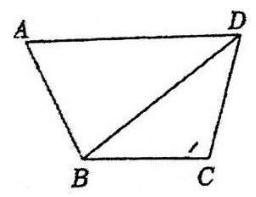
\includegraphics[max width=0.2\textwidth]{images/bo_d5jm9o77aajc7383vmi0_130_287_1537_256_197_0.jpg}
\end{center}
\hspace*{3em} 

(2)霍尔顿发现小麦的生长和发育与分割土地面积的平方和呈正相关关系. 记 \(\bigtriangleup {ABD}\) 与 \(\bigtriangleup {CBD}\) 的面积分别为 \({S}_{1}\) 和 \({S}_{2}\) ，为了更好地规划麦田，请你帮助霍尔顿求出 \({S}_{1}^{2} + {S}_{2}^{2}\) 的最大值

【解析】(1) 在 \(\bigtriangleup {ABD}\) 中, \(B{D}^{2} = A{D}^{2} + A{B}^{2} - {2AD} \cdot  {AB}\cos A = 5 - 4\cos A\)

在 \({\Delta BCD}\) 中, \(B{D}^{2} = C{D}^{2} + C{B}^{2} - {2CD} \cdot  {CB}\cos C = 2 - 2\cos C\) ,

所以 \(4\cos A - 3 = 2\cos C\) ,则 \(2\cos A - \cos C = \frac{3}{2}\) 为定值

(2) \({S}_{1}^{2} + {S}_{2}^{2} = \frac{1}{4}{A{B}^{2}} \cdot  {A{D}^{2}} \cdot  {\sin }^{2}A + \frac{1}{4}{B{C}^{2}} \cdot  {C{D}^{2}} \cdot  {\sin }^{2}C = {\sin }^{2}A + \frac{1}{4}{\sin }^{2}C\)

\(= {\sin }^{2}A + \frac{1}{4} - \frac{1}{4}{\cos }^{2}C = \left( {1 - {\cos }^{2}A}\right)  + \frac{1}{4} - \frac{1}{4}{\left( 2\cos A - \frac{3}{2}\right) }^{2}\)

\(=  - 2{\cos }^{2}A + \frac{3}{2}\cos A + \frac{11}{16}\) ,

因为 \(A \in  \left( {0,\pi }\right)\) ,设 \(t = \cos A \in  \left( {-1,1}\right)\) ,

则 \(y =  - 2{t}^{2} + \frac{3}{2}t + \frac{11}{16} =  - 2{\left( t - \frac{3}{8}\right) }^{2} + \frac{31}{32},t \in  \left( {-1,1}\right)\) ,

所以,当 \(t = \frac{3}{8} \in  \left( {-1,1}\right)\) 时, \(y =  - 2{t}^{2} + \frac{3}{2}t + \frac{11}{16}\) 取得最大值 \(\frac{31}{32}\) ,

即 \(\cos A = \frac{3}{8}\) 时, \({S}_{1}^{2} + {S}_{2}^{2}\) 的最大值为 \(\frac{31}{32}\)

\section*{板块三:中档主观题}

\section*{1. 真题回顾}

【例题】1. (2023 上海春考) 已知 \(S\) 为正比例系数,定义: \(S = \frac{{F}_{0}}{{V}_{0}},{F}_{0}\) 为建筑物暴露在空气中的面积 (单位:平方米), \({V}_{0}\) 为建筑物的体积 (单位:立方米).

(1)若有一个圆柱体建筑的底面半径为 \(R\) ，高度为 \(H\) ，求该建筑体的 \(S\) 的值 (用 \(R\) 、 \(H\) 表示)；

(2)现有一个建筑体，侧面皆垂直于地面，设 \(A\) 为底面面积， \(L\) 为建筑底面周长. 已知 \(f\) 为正比例系数, \({L}^{2}\) 与 \(A\) 成正比,定义: \(f = \frac{{L}^{2}}{A}\) ,建筑面积即为每一层的底面面积,总建筑面积即为每层建筑面积之和,值为 \(T\) .

已知该建筑体推导得出 \(S = \sqrt{\frac{f \cdot  n}{T}} + \frac{1}{3n},n\) 为层数,层高为 3 米,其中 \(f = {18},T = {10000}\) ,试求当取第几层时,该建筑体 \(S\) 最小?

【解析】(1) \(S = \frac{\pi {R}^{2} + {2\pi RH}}{\pi {R}^{2}H} = \frac{1}{H} + \frac{2}{R}\) ;

(2) \(S = \sqrt{\frac{18n}{10000}} + \frac{1}{3n} = \frac{3\sqrt{2} \cdot  \sqrt{n}}{100} + \frac{1}{3n},{S}^{\prime } = \frac{3\sqrt{2}}{{200}\sqrt{n}} - \frac{1}{3{n}^{2}}\) ,

令 \({S}^{\prime } = 0\) ,得 \({S}^{\prime } = 0 \Rightarrow  n = \sqrt[\frac{3}{2}]{\frac{200}{9\sqrt{2}}} \approx  {6.27}\) .

当 \(n = 6\) 时, \(S = {0.1594}\) ,当 \(n = 7\) 时, \(S = {0.1598}\) ,

所以当 \(n = 6\) 时,建筑体 \(S\) 最小.

【例题】2. (2022 上海春考) 为有效塑造城市景观、提升城市环境品质, 上海市正在努力推进新一轮架空线入地工程的建设. 如图是一处要架空线入地的矩形地块 \({ABCD},{AB} = {30m},{AD} = {15m}\) . 为保护 \(D\) 处的一棵古树,有关部门划定了以 \(D\) 为圆心、 \({DA}\) 为半径的四分之一圆的地块为历史古迹封闭区. 若架空线入线口为 \({AB}\) 边上的点 \(E\) ，出线口为 \({CD}\) 边上的点 \(F\) ，施工要求 \({EF}\) 与封闭区边界相切， \({EF}\) 右侧的四边形地块 \({BCFE}\) 将作为绿地保护生态区. (计算长度精确到 \({0.1}\mathrm{\;m}\) ,计算面积精确到 \({0.01}{\mathrm{\;m}}^{2}\) ).

\begin{center}
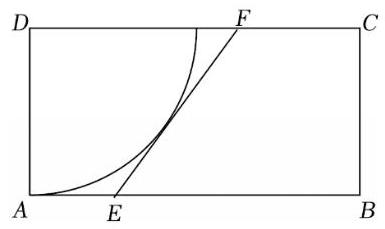
\includegraphics[max width=0.3\textwidth]{images/bo_d5jm9o77aajc7383vmi0_132_1071_1147_385_229_0.jpg}
\end{center}
\hspace*{3em} 

(1)若 \(\angle {ADE} = {20}^{ \circ  }\) ，求 \({EF}\) 的长；

(2) 当入线口 \(E\) 在 \({AB}\) 上的什么位置时,生态区的面积最大? 最大面积是多少?

【解析】(1) 法一:若 \(\angle {ADE} = {20}^{ \circ  }\) ，则 \(\angle {AEG} = 2\left( {{90}^{ \circ  } - {20}^{ \circ  }}\right)  = {140}^{ \circ  }\) ，

所以 \(\angle {BEF} = {40}^{ \circ  }\) ，所以 \({EF} = \frac{BC}{\sin {40}^{ \circ  }} = \frac{15}{\sin {40}^{ \circ  }} \approx  {23.3}\) 米；

法二:若 \(\angle {ADE} = {20}^{ \circ  }\) ，则 \(\angle {EDG} = {20}^{ \circ  }\) ， \(\angle {GDF} = {50}^{ \circ  }\) ，

所以 \({EF} = {EG} + {GF} = {15}\tan {20}^{ \circ  } + {15}\tan {50}^{ \circ  } \approx  {23.3}\) 米;

(2)法一:设 \(\angle {FEH} = \theta\) ， \(\theta  \in  \left( {0,\frac{\pi }{2}}\right)\) ，

则 \(\angle {DFE} = \theta\) ,且 \({DF} = \frac{DG}{\sin \theta } = \frac{15}{\sin \theta },{EH} = \frac{15}{\tan \theta }\) ,

得 \({CF} = {30} - \frac{15}{\sin \theta },{BE} = \frac{15}{\tan \theta } - \frac{15}{\sin \theta } + {30}\)

所以梯形面积 \(S = \frac{1}{2}\left( {{30} - \frac{15}{\sin \theta } + \frac{15}{\tan \theta } - \frac{15}{\sin \theta } + {30}}\right)  \cdot  {15}\)

\(= \frac{15}{2}\left\lbrack  {{60} - {15} \cdot  \frac{2 - \cos \theta }{\sin \theta }}\right\rbrack  ,\)

设 \(m = \frac{2 - \cos \theta }{\sin \theta }\) ,则 \(m\sin \theta  + \cos \theta  = 2\) ,所以 \(\sqrt{{m}^{2} + 1}\sin \left( {\theta  + \varphi }\right)  = 2\) ,

所以 \(\sin \left( {\theta  + \varphi }\right)  = \frac{2}{\sqrt{{m}^{2} + 1}} \leq  1\) ,得 \(m \geq  \sqrt{3}\) ,其中 \(\tan \varphi  = \frac{1}{m}\) ,

所以 \({S}_{\max } = \frac{15}{2}\left( {{60} - {15}\sqrt{3}}\right)  \approx  {255.14}\) 平方米,当且仅当 \(\theta  = \frac{\pi }{6}\) 时取等号.

此时 \({EH} = \frac{15}{\tan {30}^{ \circ  }} = {15}\sqrt{3},{CF} = {30} - \frac{15}{\sin {30}^{ \circ  }} = 0\) ,

所以 \({AE} = {30} - {15}\sqrt{3}\) 米;

法二: 以 \(D\) 为原点建系,设切点 \(G\left( {{x}_{0},{y}_{0}}\right)\) ,令 \(\left\{  {\begin{array}{l} {x}_{0} = {15}\cos \theta \\  {y}_{0} = {15}\sin \theta  \end{array},\theta  \in  \left( {-\frac{\pi }{3},0}\right\rbrack  }\right.\) ,

则切线 \({EF}\) 的方程为 \({x}_{0}x + {y}_{0}y = {15}^{2}\) ,令 \(y = 0\) ,得 \(x = \frac{{15}^{2}}{{x}_{0}}\) ,

令 \(y =  - {15}\) ,得 \(x = \frac{{15}^{2} + {15}{y}_{0}}{{x}_{0}}\) ,所以 \(E\left( {\frac{{15}^{2} + {15}{y}_{0}}{{x}_{0}}, - {15}}\right) ,F\left( {\frac{{15}^{2}}{{x}_{0}},0}\right)\) ,

所以梯形面积 \(S = \left( {{60} - \frac{{15}^{2}}{{x}_{0}} - \frac{{15}^{2} + {15}{y}_{0}}{{x}_{0}}}\right)  \cdot  \frac{15}{2} = {450} - \frac{225}{2} \cdot  \frac{{30} + {y}_{0}}{{x}_{0}}\)

\(= {450} - \frac{225}{2} \cdot  \frac{2 + \sin \theta }{\cos \theta }\) ,

设 \(m = \frac{2 + \sin \theta }{\cos \theta }\) ,则 \(\sin \theta  - m\cos \theta  =  - 2\) ,所以 \(\sqrt{{m}^{2} + 1}\sin \left( {\theta  + \varphi }\right)  =  - 2\) ,

所以 \(\sin \left( {\theta  + \varphi }\right)  = \frac{-2}{\sqrt{{m}^{2} + 1}} \geq   - 1\) ,得 \(m \geq  \sqrt{3}\) ,其中 \(\tan \varphi  =  - m\) ,

所以 \({S}_{\max } = {450} - \frac{225}{2} \cdot  \sqrt{3} \approx  {255.14}\) 平方米,当且仅当 \(\theta  =  - \frac{\pi }{6}\) 时取等号.

此时 \({EH} = \frac{15}{\tan {30}^{ \circ  }} = {15}\sqrt{3},{CF} = {30} - \frac{15}{\sin {30}^{ \circ  }} = 0\) ,

所以 \({AE} = {{30} - {15}\sqrt{3}}\) 米；

法三: 设 \(\angle {ADE} = \theta\) ，则 \({AE} = {15}\tan \theta\) ，

\({DF} = {AE} + \frac{AD}{\tan {2\theta }} = {15}\tan \theta  + \frac{15}{\tan {2\theta }}\)

所以梯形面积 \(S = \frac{1}{2}\left( {{30} - {15}\tan \theta  + {30} - {15}\tan \theta  - \frac{15}{\tan {2\theta }}}\right)  \cdot  {15}\)

\(= \frac{15}{2}\left( {{60} - {30}\tan \theta  - \frac{{15}\left( {1 - {\tan }^{2}\theta }\right) }{2\tan \theta }}\right)  = \frac{15}{2}\left\lbrack  {{60} - \frac{15}{2}\left( {3\tan \theta  + \frac{1}{\tan \theta }}\right) }\right\rbrack\)

\(\leq  \frac{15}{2}\left( {{60} - \frac{15}{2} \cdot  2\sqrt{3}}\right)  \approx  {255.14}\) ,当且仅当 \(\theta  = \frac{\pi }{6}\) 时取等号,

此时 \({EH} = \frac{15}{{\operatorname{tan30}}^{ \circ  }} = {15}\sqrt{3},{CF} = {30} - \frac{15}{{\operatorname{sin30}}^{ \circ  }} = 0\) ,

所以 \({AE} = {30} - {15}\sqrt{3}\) 米.

【注】上述法一和法二中,涉及 \(m = \frac{2 - \cos \theta }{\sin \theta }\) 和 \(m = \frac{2 + \sin \theta }{\cos \theta }\) 的计算,除了使用辅助角公式,还可以看成斜率或者使用万能公式去处理, 下面写出详细过程.

对于 \(m = \frac{2 - \cos \theta }{\sin \theta }\) ,看成 \(P\left( {0,2}\right)\) 和单位圆上的点 \(\left( {-\sin \theta ,\cos \theta }\right)\) 连线的斜率,设与单位圆相切的直线为 \(y = {kx} + 2\) ,则 \(\frac{2}{\sqrt{{k}^{2} + 1}} = 1\) ,所以 \(k =  \pm  \sqrt{3}\) ,考虑题目条件,取 \(k = \sqrt{3}\) ; 亦可以考虑 \({OP} = 2\) 为两倍的半径,在直角三角形中,由三边关系直接得出相切的斜率 \(k = \sqrt{3}\) ;

另外,令 \(t = \tan \frac{\theta }{2}\) ,则 \(m = \frac{2 - \cos \theta }{\sin \theta } = \frac{2 - \frac{1 - {\tau }^{2}}{1 + {t}^{2}}}{\frac{2t}{1 + {t}^{2}}} = \frac{1 + 3{t}^{2}}{2t} = \frac{1}{2t} + \frac{3t}{2} \geq  \sqrt{3}\) ,当且仅当 \(t = \; \frac{\sqrt{3}}{3}\) 时取等号. 对于另一个式子也可以这样处理.

【例题】3. (2021 上海春考)(1)团队在 \(O\) 点西侧、东侧 20 千米处设有 \(A\) 、 \(B\) 两站点,测量距离发现一点 \(P\) 满足 \(\left| {PA}\right|  - \left| {PB}\right|  = {20}\) 千米,可知 \(P\) 在 \(A\text{ 、 }B\) 为焦点的双曲线上,以 \(O\) 点为原点,东侧为 \(x\) 轴正半轴,北侧为 \(y\) 轴正半轴,建立平面直角坐标系, \(P\) 在北偏东 \({60}^{ \circ  }\) 处,求双曲线标准方程和 \(P\) 点坐标.

(2)团队又在南侧、北侧 15 千米处设有 \(C\) 、 \(D\) 两站点，测量距离发现 \(\left| {QA}\right|  - \left| {QB}\right|  = {30}\) 千米， \(\left| {QC}\right|  - \left| {QD}\right|  = {10}\) 千米,求 \(\left| {OQ}\right|\) (精确到 1 米) 和 \(Q\) 点位置 (精确到 1 米, \(\left. {1}^{ \circ  }\right)\) .

【解析】(1) 由题意得 \(a = {10},c = {20}\) ,所以 \({b}^{2} = {300}\) ,

所以双曲线的标准方程为 \(\frac{{x}^{2}}{100} - \frac{{y}^{2}}{300} = 1\) ,

直线 \({OP} : y = \frac{\sqrt{3}}{3}x\) ,联立双曲线方程,得 \(x = \frac{{15}\sqrt{2}}{2},y = \frac{5\sqrt{6}}{2}\) ,

即点 \(P\) 的坐标为 \(\left( {\frac{{15}\sqrt{2}}{2},\frac{5\sqrt{6}}{2}}\right)\) .

(2) \circled{1}  \(\left| {QA}\right|  - \left| {QB}\right|  = {30}\) ，则 \(a = {15}\) ， \(c = {20}\) ，所以 \({b}^{2} = {175}\) ，

双曲线方程为 \(\frac{{x}^{2}}{225} - \frac{{y}^{2}}{175} = 1\) ;

 \circled{2}  \(\left| {QC}\right|  - \left| {QD}\right|  = {10}\) ，则 \(a = 5\) ， \(c = {15}\) ，所以 \({b}^{2} = {200}\) ，

所以双曲线方程为 \(\frac{{y}^{2}}{25} - \frac{{x}^{2}}{200} = 1\) ,

两双曲线方程联立，得 \(Q\left( {\sqrt{\frac{14400}{47}},\sqrt{\frac{2975}{47}}}\right)\) ，

所以 \(\left| {OQ}\right|  \approx  {19}\) 米, \(Q\) 点位置北偏东 \({66}^{ \circ  }\) .

【例题】4. (2020 上海春考) 有一条长为 120 米的步行道 \({OA},A\) 是垃圾投放点 \({\omega }_{1}\) ,若以 \(O\) 为原点, \({OA}\) 为 \(x\) 轴正半轴建立直角坐标系,设点 \(B\left( {x,0}\right)\) ,现要建设另一座垃圾投放点 \({\omega }_{2}\left( {t,0}\right)\) ,函数 \({f}_{t}\left( x\right)\) 表示与 \(B\) 点距离最近的垃圾投放点的距离.

(1) 若 \(t = {60}\) ，求 \({f}_{60}\left( {10}\right)\) 、 \({f}_{60}\left( {80}\right)\) 、 \({f}_{60}\left( {95}\right)\) 的值，并写出 \({f}_{60}\left( x\right)\) 的函数解析式；

(2)若可以通过 \({f}_{t}\left( x\right)\) 与坐标轴围成的面积来测算扔垃圾的便利程度，面积越小越便利. 问:垃圾投放点 \({\omega }_{2}\) 建在何处才能比建在中点时更加便利?

【解析】(1) 投放点 \({\omega }_{1}\left( {{120},0}\right) ,{\omega }_{2}\left( {{60},0}\right) ,{f}_{60}\left( {10}\right)\) 表示与 \(B\left( {{10},0}\right)\) 距离最近的投放点

(即 \({\omega }_{2}\) ) 的距离,所以 \({f}_{60}\left( {10}\right)  = \left| {{60} - {10}}\right|  = {50}\) ,

同理可得, \({f}_{60}\left( {80}\right)  = \left| {{60} - {80}}\right|  = {20},{f}_{60}\left( {95}\right)  = \left| {{120} - {95}}\right|  = {25}\) ,

由题意得 \({f}_{60}\left( x\right)  = \{ \left| {{60} - x}\right| ,\left| {{120} - x}\right| {\} }_{\min }\) ,

则当 \(\left| {{60} - x}\right|  \leq  \left| {{120} - x}\right|\) ,即 \(x \leq  {90}\) 时, \({f}_{60}\left( x\right)  = \left| {{60} - x}\right|\) ;

当 \(\left| {{60} - x}\right|  > \left| {{120} - x}\right|\) ,即 \(x > {90}\) 时, \({f}_{60}\left( x\right)  = \left| {{120} - x}\right|\) ;

综上, \({f}_{60}\left( x\right)  = \left\{  \begin{array}{ll} \left| {{60} - x}\right| , & x \leq  {90} \\  \left| {{120} - x}\right| , & x > {90} \end{array}\right.\) ;

(2)由题意得 \({f}_{t}\left( x\right)  = {\left\{  \left| t - x\right| ,\left| {120} - x\right| \right\}  }_{\min }\) ， 2025 版上海高考真题及模拟训练合集(下册)

\begin{center}
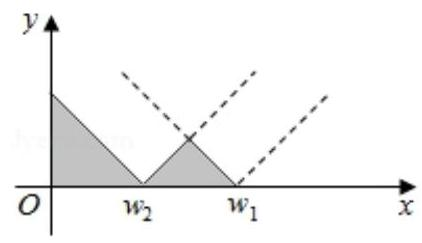
\includegraphics[max width=0.3\textwidth]{images/bo_d5jm9o77aajc7383vmi0_135_1027_259_422_243_0.jpg}
\end{center}
\hspace*{3em} 

所以 \({f}_{t}\left( x\right)  = \left\{  \begin{array}{l} \left| {t - x}\right| ,x \leq  {0.5}\left( {{120} + t}\right) \\  \left| {{120} - x}\right| ,x > {0.5}\left( {{120} + t}\right)  \end{array}\right.\) ,

则 \({f}_{t}\left( x\right)\) 与坐标轴围成的面积如阴影部分所示,

所以 \(S = \frac{1}{2}{t}^{2} + \frac{1}{4}{\left( {120} - t\right) }^{2} = \frac{3}{4}{t}^{2} - {60t} + {3600}\) ,

由题意得 \(S < S\left( {60}\right)\) ,

即 \(\frac{3}{4}{t}^{2} - {60t} + {3600} < {2700}\) ,

解得 \({20} < t < {60}\) ,即垃圾投放点 \({\omega }_{2}\) 建在 \(\left( {{20},0}\right)\) 与 \(\left( {{60},0}\right)\) 之间时,比建在中点时更加便利.

【例题】5. (2018 上海春考) 利用“平行于圆锥母线的平面截圆锥面, 所得截线是抛物线”的几何原理, 某快餐店用两个射灯 (射灯的光锥为圆锥) 在广告牌上投影出其标识, 如图 1 所示, 图 2 是投影射出的抛物线的平面图,图 3 是一个射灯投影的直观图,在图 2 与图 3 中,点 \(O\text{ 、 }A\text{ 、 }B\) 在抛物线上, \({OC}\) 是抛物线的对称轴, \({OC} \bot  {AB}\) 于 \(C,{AB} = 3\) 米, \({OC} = {4.5}\) 米

(1)求抛物线的焦点到准线的距离

(2)在图 3 中，已知 \({OC}\) 平行于圆锥的母线 \({SD},{AB}\text{ 、 }{DE}\) 是圆锥底面的直径，求圆锥的母线与轴的夹角的大小 (精确到 \({0.01}^{ \circ  }\) )

\begin{center}
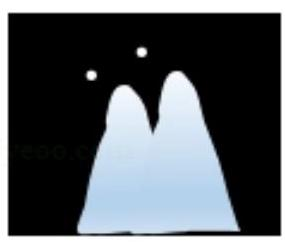
\includegraphics[max width=0.2\textwidth]{images/bo_d5jm9o77aajc7383vmi0_135_322_983_285_242_0.jpg}
\end{center}
\hspace*{3em} 

图1

\begin{center}
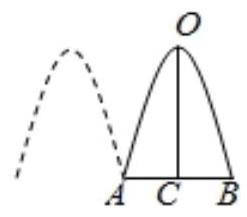
\includegraphics[max width=0.2\textwidth]{images/bo_d5jm9o77aajc7383vmi0_135_735_986_247_217_0.jpg}
\end{center}
\hspace*{3em} 

图2

\begin{center}
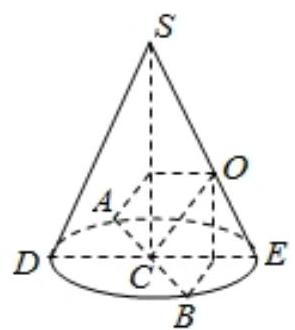
\includegraphics[max width=0.2\textwidth]{images/bo_d5jm9o77aajc7383vmi0_135_1078_926_295_330_0.jpg}
\end{center}
\hspace*{3em} 

图3

【解析】(1) 在图 2 中,以 \(O\) 为原点,以 \({OC}\) 为 \(y\) 轴负半轴建立平面直角坐标系,

设抛物线方程为 \({x}^{2} =  - {2py}\left( {p > 0}\right)\) ,由题意得 \(B\left( {\frac{3}{2}, - \frac{9}{2}}\right)\) ,

所以 \(\frac{9}{4} =  - {2p} \cdot  \left( {-\frac{9}{2}}\right)\) ,解得 \(p = \frac{1}{4}\) ,所以抛物线的焦点到准线的距离为 \(\frac{1}{4}\) .

(2)在图 3 中，因为 \({OC}//{SD}\) ，所以 \(\frac{OC}{SD} = \frac{CE}{DE} = \frac{1}{2}\) ，所以 \({SD} = {2OC} = 9\) ，

又 \({DC} = \frac{1}{2}{AB} = \frac{3}{2}\) ，所以 \(\sin \angle {CSD} = \frac{CD}{SD} = \frac{1}{6}\) .

所以圆锥的母线与轴的夹角为 \(\arcsin \frac{1}{6} \approx  {9.59}^{ \circ  }\) . 2025 版上海高考真题及模拟训练合集(下册)

\section*{2. 模拟练习}

【练习】1. (2024 届交附) 高三新教学楼启用后, 从一些教室窗口就能看到殷高路对面居民房平改坡后的屋顶 (如图). 其中 \({AB}\) 是屋脊线, \({MN}\) 是屋檐线, \({ABMN}\) 是屋顶坡面, \({CDE}\) 是一个与水平面垂直的带气窗的竖直面， \({EF}\) 是气窗屋顶的屋脊线且 \({EF}\) 与竖直面 \({CDE}\) 垂直

\begin{center}
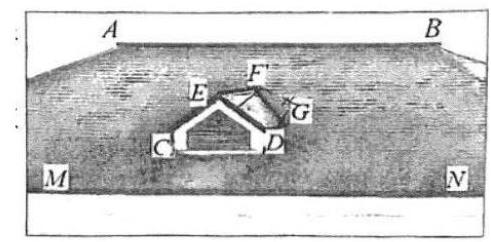
\includegraphics[max width=0.4\textwidth]{images/bo_d5jm9o77aajc7383vmi0_136_310_426_491_242_0.jpg}
\end{center}
\hspace*{3em} 

小张和小王对屋顶进行研究，提出了下面一些假设:

 \circled{1} 两条屋脊线 \({AB}\) 与 \({EF}\) 互相垂直且都与水平面平行；

 \circled{2} 气窗屋顶的两个坡面 \({EFC}\) 与 \({EFGD}\) 互相垂直且与水平面的所成角相等;

 \circled{3} 屋顶坡面 \({ABMN}\) 与水平面所成角为 \({30}^{ \circ  }\)

(1)小张认为还需假设屋脊线 \({AB}\) 与带气窗的竖直面 \({CDE}\) 是平行关系. 而小李认为前面的假设已经够了，不需要再提出这个假设. 请你判断哪位同学正确？证明你的判断

(2)根据小张和小王的假设，试求气窗屋顶的一个坡面 \({DEFG}\) 与屋顶坡面 \({ABMN}\) 构成的阴脊线 \({FG}\) (是平面 \({ABMN}\) 与平面 \({EFGD}\) 的交线) 与水平面所成角的大小. (用反三角函数表示)

【解析】(1) 不需再提假设

\begin{center}
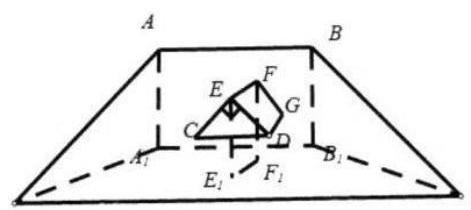
\includegraphics[max width=0.4\textwidth]{images/bo_d5jm9o77aajc7383vmi0_136_328_1090_471_210_0.jpg}
\end{center}
\hspace*{3em} 

在水平面上分别取 \(A,B,E,F\) 的射影 \({A}_{1},{B}_{1},{E}_{1},{F}_{1}\) ,

连接 \(A{A}_{1},B{B}_{1},E{E}_{1},F{F}_{1},{A}_{1}{B}_{1},{E}_{1}{F}_{1}\) ,

则 \(A,B,{A}_{1},{B}_{1}\) 四点共面，又 \({AB}//\) 水平面，平面 \({AB}{B}_{1}{A}_{1} \cap\) 水平面 \(= {A}_{1}{B}_{1}\) ，

则 \({AB}//{A}_{1}{B}_{1}\) ，同理 \({EF}//{E}_{1}{F}_{1}\) ，又 \({EF}\bot {AB}\) ，所以 \({{E}_{1}{F}_{1}}\bot {AB}\) ，

又 \(A{A}_{1} \bot\) 水平面， \({E}_{1}{F}_{1} \subset\) 水平面，则 \(A{A}_{1} \bot  {E}_{1}{F}_{1}\) ，

\(A{A}_{1} \cap  {AB} = A,A{A}_{1},{AB} \subset\) 平面 \({AB}{B}_{1}{A}_{1}\) ,则 \({E}_{1}{F}_{1} \bot\) 平面 \({AB}{B}_{1}{A}_{1}\) ,

即 \({EF} \bot\) 平面 \({AB}{B}_{1}{A}_{1}\) ,又 \({EF} \bot\) 平面 \({CDE}\) ,则平面 \({AB}{B}_{1}{A}_{1}//\) 平面 \({CDE}\) ,

因为 \({AB} \subset\) 平面 \({AB}{B}_{1}{A}_{1}\) ,所以 \({AB}//\) 平面 \({CDE}\)

(2)把气窗脱离出来，即三棱柱被斜面截到的部分即多面体 \({ECD} - {FNG}\) ，

则屋顶坡面 \({ABMN}\) 即为平面 \({FNG}\) ,如图,

\begin{center}
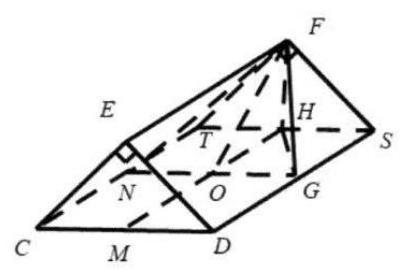
\includegraphics[max width=0.3\textwidth]{images/bo_d5jm9o77aajc7383vmi0_136_305_1776_401_270_0.jpg}
\end{center}
\hspace*{3em} 

则平面 \({CDST}//\) 水平面,分别取 \({ST},{CD}\) 中点 \(H,M\) ,连接 \({HM}\) ,

过 \(G\) 作 \({GN}//{CD}\) ,交 \({HM},{CT}\) 于 \(O,N\) ,连接 \({FO},{HG}\) ,

则 \({FH} \bot\) 平面 \({CDST},{GN} \subset\) 平面 \({CDST}\) ,则 \({FH} \bot  {GN}\) ,

又 \({CD} \bot  {HM}\) ,即 \({GN} \bot  {HM},{FH} \cap  {HO} = H\) ,

\({FH},{HO} \subset\) 平面 \({FHO}\) ,则 \({GN} \bot\) 平面 \({FHO}\) ,

又平面 \({FNG} \cap\) 平面 \({CDST} = {GN}\) ,

则 \(\angle {FOH}\) 为屋顶坡面 \({ABMN}\) 与水平面所成角为 \({30}^{ \circ  }\) ,

在 Rt \(\bigtriangleup {FHO}\) 中,设 \({FH} = 1\) ,则 \({HO} = \sqrt{3},{FO} = 2\) ,

则在等腰 \({Rt}\bigtriangleup {FHS},{HS} = 1\) ,则 \({OG} = 1\) ,

在 Rt \(\bigtriangleup {HOG},{HG} = \sqrt{H{O}^{2} + O{G}^{2}} = 2\) ,

则在 \({Rt}\bigtriangleup {FHG},{FG} = \sqrt{H{G}^{2} + F{H}^{2}} = \sqrt{5}\) ,

又 \({FH} \bot\) 平面 \({CDST}\) ,则 \({HG}\) 为 \({FG}\) 在平面 \({CDST}\) 的射影,

则 \(\angle {FGH}\) 为 \({FG}\) 与水平面所成角，则 \(\sin \angle {FGH} = \frac{FH}{FG} = \frac{1}{\sqrt{5}} = \frac{\sqrt{5}}{5}\) ，

则 \({FG}\) 与水平面所成角为 \(\arcsin \frac{\sqrt{5}}{5}\)

【练习】2. (2025 届交附) 仰晖楼有 \(A,B\) 两部电梯. 已知电梯每上一层需要 5 秒，电梯在某层楼停留时开门到关门所花时间为 10 秒 (人员均能在电梯开关门时间内完成进出电梯和按楼层等操作).

某天清晨，楼上还没有人，1楼已经有若干人均欲乘坐电梯上楼，目的地分别是 2 到 10 楼.

现两部电梯均恰好在 1 楼 (两部电梯互相独立运行, 可以独立开关门, 在 1 楼按下按钮后将同时打开门),且每部电梯容量足够容纳所有人. 定义 \({T}_{A}\left( {T}_{B}\right)\) 为: 从 \(A\left( B\right)\) 电梯开门时刻算起,到电梯内最后一人到达目标楼层后 \(A\left( B\right)\) 电梯门关闭为止,所花时间.

记“运输完成时间”: \({T}_{0} = \max \left\{  {{T}_{A},{T}_{B}}\right\}\)

(1)若所有人均乘坐一部电梯，求 \({T}_{0}\) ；

(2)为了研究 \({T}_{0}\) 的最小值，我们需要对电梯的“乘坐安排”作出一些合理假设. 例如:假设两部电梯都有人乘坐. 理由: 分开乘坐,比如去 2 层的人都坐电梯 \(A\) ,其余人坐电梯 \(B\) ,则 \({T}_{A},{T}_{B}\) 均小于 (1) 中 \({T}_{0}\) ，故 “运输完成时间” 也小于 (1) 中 \({T}_{0}\) ，所以要使得 \({T}_{0}\) 最小，

两部电梯一定都有人乘坐. 请你在此基础上再提出 1 至 2 条关于电梯 “乘坐安排”的合理假设, 并简述作出这些假设的理由 (若有多条假设, 请按重要性从高到低写出最重要的两条);

(3) 求出 \({T}_{0}\) 最小值

【解析】(1) 包括 1 楼, 电梯共开关门 10 次数, 上升 9 层,

所以完成运输所花时间为 \({10} \times  {10} + 9 \times  5 = {145}\) 秒;

(2)假设一:目的地为同一层楼的人都坐同一部电梯，

即 \(A,B\) 电梯所到楼层不重叠

理由:将目的地为同一层楼的人调整到同一部电梯可以使得其中一部电梯至少节约 10 秒，这样调整后方案的“运输完成时间”必然不大于原方案. 假设二:不妨设 \(A\) 电梯到达 10 层，

则可假设 \(B\) 电梯停留层数均小于 \(A\) 电梯停留层数

理由: 记 \(B\) 电梯最高到达 \(b\left( {b < {10}}\right)\) 楼,若存在 \(A\) 电梯到达 \(a\) 楼,

且 \(a < b\) 的情况. 两部电梯交换这两层的人，则 \({T}_{A}\) 不变， \({T}_{B}\) 至少减少 5 秒，

新方案“运输完成时间”必然不大于原方案；

(3) 设 \(A\) 电梯到达楼层为 \(a \sim  {10}\) 层, \({10} \geq  a \geq  3,B\) 电梯到达楼层为 \(2 \sim  a - 1\) 层,

\({T}_{A} = \left( {{12} - a}\right)  \times  {10} + 9 \times  5 = {165} - {10a},\)

\({T}_{B} = \left( {a - 1}\right)  \times  {10} + \left( {a - 2}\right)  \times  5 = {15a} - {20},\)

\({T}_{0} = \max \left\{  {{T}_{A},{T}_{B}}\right\}   = \left\{  \begin{array}{l} {165} - {10a},3 \leq  a \leq  7 \\  {15a} - {20},8 \leq  a \leq  {10} \end{array}\right.\)

当 \(a = 7\) 时， \({T}_{0}\) 取得最小值 95 秒，

即 \(A\) 电梯目的地为 710 层， \(B\) 电梯目的地为 2 \textasciitilde  6 层

【练习】3. 机器人竞技是继电子竞技之后热门的科技竞技项目，某区为了参加市机器人竞技总决赛， 开展了区内选行场比赛互相独立下表统计的是 \(A\) 在近期热身中分别与 \(B,C,D\) 三人比赛的情况.

\begin{center}
\adjustbox{max width=\textwidth}{
\begin{tabular}{|c|c|c|c|}
\hline
\phantom{X} & \(B\) & \(C\) & \(D\) \\
\cline{1-4}
比赛的次数 & 12 & 10 & 15 \\
\cline{1-4}
\(A\) 获胜的次数 & 4 & 5 & 12 \\
\cline{1-4}
\hline
\end{tabular}
}
\end{center}

(1)根据表格中的数据，试估计在区内决赛中 \(A\) 至少获胜一场的概率；

(2)根据表格中的数据，请给 \(B,C,D\) 三人设计一个出场顺序，使得 \(A\) 在这三场比赛中连胜两场的概率最大, 并说明理由.

【解析】(1)由热身赛统计情况,估计 \(A\) 与 \(B,A\) 与 \(C,A\) 与 \(D\) 比赛时获胜的概率

分别记为 \({P}_{1},{P}_{2},{P}_{3}\) ,

依据表格中的数据得 \({P}_{1} = \frac{4}{12} = \frac{1}{3},{P}_{2} = \frac{5}{10} = \frac{1}{2},{P}_{3} = \frac{12}{15} = \frac{4}{5}\) , 3 分

记“在区内决赛中 \(A\) 至少获胜一场”为事件 \(M\) ,

则 \(P\left( M\right)  = 1 - P\left( \bar{M}\right)  = 1 - \left( {1 - {P}_{1}}\right) \left( {1 - {P}_{2}}\right) \left( {1 - {P}_{3}}\right)  = 1 - \frac{2}{3} \times  \frac{1}{2} \times  \frac{1}{5} = \frac{14}{15}\) ,

则估计在区内决赛中 \(A\) 至少获胜一场的概率为 \(\frac{14}{15}\) . 6 分

(2)若 \(B\) 在第二位出场，即出场顺序为 \({CBD}\) 或 \({DBC}\) ，

则 \(A\) 在这三场比赛中连胜两场的概率为 \(\frac{1}{2} \times  \frac{1}{3} \times  \left( {1 - \frac{4}{5}}\right)  + \left( {1 - \frac{1}{2}}\right)  \times  \frac{1}{3} \times  \frac{4}{5} = \frac{1}{6}\)

或 \(\frac{4}{5} \times  \frac{1}{3} \times  \left( {1 - \frac{1}{2}}\right)  + \left( {1 - \frac{4}{5}}\right)  \times  \frac{1}{3} \times  \frac{1}{2} = \frac{1}{6}\) 2 分

若 \(C\) 在第二位出场，即出场顺序为 \({BCD}\) 或 \({DCB}\) ，

则 \(A\) 在这三场比赛中连胜两场的概率为

\(\frac{1}{3} \times  \frac{1}{2} \times  \left( {1 - \frac{4}{5}}\right)  + \left( {1 - \frac{1}{3}}\right)  \times  \frac{1}{2} \times  \frac{4}{5} = \frac{3}{10}\)

或 \(\frac{4}{5} \times  \frac{1}{2} \times  \left( {1 - \frac{1}{3}}\right)  + \left( {1 - \frac{4}{5}}\right)  \times  \frac{1}{2} \times  \frac{1}{3} = \frac{3}{10}\) 4 分

若 \(D\) 在第二位出场，即出场顺序为 \({BDC}\) 或 \({CDB}\) ,

则 \(A\) 在这三场比赛中连胜两场的概率为 \(\frac{1}{3} \times  \frac{4}{5} \times  \left( {1 - \frac{1}{2}}\right)  + \left( {1 - \frac{1}{3}}\right)  \times  \frac{1}{2} \times  \frac{4}{5} = \frac{2}{5}\)

或 \(\frac{1}{2} \times  \frac{4}{5} \times  \left( {1 - \frac{1}{3}}\right)  + \left( {1 - \frac{1}{2}}\right)  \times  \frac{4}{5} \times  \frac{1}{2} = \frac{2}{5}\) 6 分

则当 \(B,C,D\) 三人的出场顺序为 \({BDC}\) 或 \({CDB}\) 时,

\(A\) 在这三场比赛中连胜两场的概率最大. 8 分

【练习】4. (2024 届交附) 设一个简单几何体的表面积为 \(S\) ,体积为 \(V\) ,定义系数 \(K = \frac{{S}^{3}}{{V}^{2}}\) . 已知球体对应的系数为 \({K}_{0}\) ，定义 \(f = \frac{{K}_{0}}{K}\) 为一个几何体的“球形比例系数”

(1)计算正方体和正四面体的“球形比例系数”;

(2)求圆柱体的“球形比例系数”范围

(3)是否存在“球形比例系数”为0.75的简单几何体？若存在，请描述该几何体的基本特征; 若不存在, 说明理由

【解析】 \(\left( 1\right) {K}_{0} = \frac{{\left( 4\pi {r}^{2}\right) }^{3}}{{\left( \frac{4}{3}\pi {r}^{3}\right) }^{2}} = {36\pi }\) ,正方体的系数为 \({K}_{1} = \frac{{\left( 6{a}^{2}\right) }^{3}}{{\left( {a}^{3}\right) }^{2}} = {216}\) ,

正四面体的系数为 \({K}_{2} = \frac{{\left( \sqrt{3}{a}^{2}\right) }^{3}}{{\left( \frac{\sqrt{2}}{12}{a}^{3}\right) }^{2}} = {216}\sqrt{3}\)

所以,正方体 “球形比例系数” \(f = \frac{\pi }{6}\) ,

正四面体的“球形比例系数” \(f = \frac{\sqrt{3}\pi }{18}\)

(2)设圆柱底面半径为 \(r\) ,高为 \(h\) ,则全面积为 \(S = {2\pi r}\left( {r + h}\right)\) ，体积为 \(V = \pi {r}^{2}h\) ，

于是 \(K = \frac{{s}^{3}}{{V}^{2}} = {8\pi }\frac{{\left( {r}^{2} + rh\right) }^{3}}{{\left( {r}^{2}h\right) }^{2}} = {8\pi }\frac{{\left( 1 + \frac{h}{r}\right) }^{3}}{{\left( \frac{h}{r}\right) }^{2}}\) ,

设 \(x = \frac{\hslash }{r},f\left( x\right)  = \frac{{\left( 1 + x\right) }^{3}}{{x}^{2}}\) ,则 \({f}^{\prime }\left( x\right)  = \frac{x{\left( 1 + x\right) }^{2}\left( {x - 2}\right) }{{x}^{4}}\)

即 \(x \in  \left( {0,2}\right)\) 时, \(f\left( x\right)\) 单调递减; \(x \in  \left( {2, + \infty }\right)\) 时, \(f\left( x\right)\) 单调递增,

即 \(x = 2,h = {2r}\) 时,圆柱体的系数最小为 \(K = {54\pi }\) ,

所以,圆柱体的球形比例系数的值域为 \(\left( {0,\frac{2}{3}}\right\rbrack\)

(3)考虑圆柱和半球的组合体，底面重合，半径为 \(r\) ,圆柱的高为 \(h\) ， \(x = \frac{h}{r}\) ，

于是组合体的全面积 \(S = {3\pi }{r}^{2} + {2\pi rh}\) ,体积 \(V = \frac{2}{3}\pi {r}^{3} + \pi {r}^{2}h\)

\(K = \frac{{S}^{3}}{{V}^{2}} = \frac{{\left( 3\pi {r}^{2} + 2\pi rh\right) }^{3}}{{\left( \frac{2}{3}\pi {r}^{3} + \pi {r}^{2}\hslash \right) }^{2}} = {9\pi }\frac{{\left( 3 + 2x\right) }^{3}}{{\left( 2 + 3x\right) }^{2}},f\left( x\right)  = \frac{{K}_{0}}{K} = \frac{4{\left( 2 + 3x\right) }^{2}}{{\left( 3 + 2x\right) }^{3}},\)

\(f\left( 1\right)  = \frac{4}{5} > \frac{3}{4}\) ,而 \(f\left( 2\right)  = \frac{256}{343} < \frac{3}{4}\) ,当 \(x \approx  {1.95}\) 时, \(f\left( {1.95}\right)  \approx  {0.75}\cdots {14}\) 分

故存在球形比例系数为 \(\frac{3}{4}\) 的几何体,圆柱和一个半球组合而成,

底面半径相同，圆柱的高约为半径的 1.95 倍

(举例构造几何体不唯一，如还可以是中间为圆柱，两头是均为半球的组合体)

(考虑两个半球,中间一个圆柱,底面与半球大圆面重合,设半径为 \(r\) ,

圆柱的高为 \(h\) ,则组合体的全面积 \(S = {4\pi }{r}^{2} + {2\pi rh}\) ,体积 \(V = \frac{4}{3}\pi {r}^{3} + \pi {r}^{2}h\) ,

设 \(x = \frac{\hslash }{r},K = \frac{{s}^{3}}{{V}^{2}} = \frac{{\left( 4\pi {r}^{2} + 2\pi r\lambda \right) }^{3}}{{\left( \frac{4}{3}\pi {r}^{3} + \pi {r}^{2}?\right) }^{2}} = {9\pi }\frac{{\left( 4 + 2x\right) }^{3}}{{\left( 4 + 3x\right) }^{2}},f\left( x\right)  = \frac{{K}_{0}}{K} = \frac{{\left( 4 + 3x\right) }^{2}}{2{\left( 2 + x\right) }^{3}}\) ,

\(f\left( 1\right)  \approx  {0.9} > \frac{3}{4}\) ,而 \(f\left( 3\right)  \approx  {0.676} < \frac{3}{4}\) ,当 \(x \approx  {2.27}\) 时, \(f\left( {2.27}\right)  \approx  {0.75})\)

【练习】5. (2024 届交附) 某汽车企业由于产品转型不理想, 订单大量减少, 现采取 “减员增效” 中对部分人员实行分流，规定分流人员第一年可以到原单位领取工资的 100\%，从第二年起，以后每年只能在原单位按上一年的 \(\frac{2}{3}\) 领取工资，该厂根据分流人员的技术特长，计划创办新的经济实体,该经济实体预计第一年属投资阶段,第二年每人可获得 \(b\) 元收入,从第三年起每人每年的收入可在上一年的基础上递增 50\%,如果某人分流前工资的收入每年 \(a\) 元,分流后进入新经济实体,第 \(n\) 年的收入为 \({a}_{n}\) 元 (第一年,参与经济体的人员没有收入)

(1)求 \(\left\{  {a}_{n}\right\}\) 的通项公式；

(2) 当 \(b = \frac{8a}{27}\) 时,这个人哪一年的收入最少? 最少为多少?

(3)当 \(b \geq  \frac{3a}{8}\) 时，是否一定可以保证这个人分流一年后的收入永远超过分流前的年收入？

【解析】(1) 由题意得,当 \(n = 1\) 时, \({a}_{1} = a\) ,

当 \(n \geq  2\) 时, \({a}_{n} = a{\left( \frac{2}{3}\right) }^{n - 1} + b{\left( \frac{3}{2}\right) }^{n - 2}\) ,

所以 \({a}_{n} = \left\{  \begin{array}{ll} a & \left( {n = 1}\right) \\  a{\left( \frac{2}{3}\right) }^{n - 1} + b{\left( \frac{3}{2}\right) }^{n - 2} & \left( {n \geq  2}\right)  \end{array}\right.\)

(2)由已知 \(b = \frac{8a}{27}\) ，

当 \(n \geq  2\) 时， \({a}_{n} = a{\left( \frac{2}{3}\right) }^{n - 1} + \frac{8a}{27}{\left( \frac{3}{2}\right) }^{n - 2} \geq  2{\left\lbrack  a{\left( \frac{2}{3}\right) }^{n - 1} \times  \frac{8a}{27}{\left( \frac{3}{2}\right) }^{n - 2}\right\rbrack  }^{\frac{1}{2}} = \frac{8a}{9}\) ，

要使得上式等号成立,当且仅当 \(a{\left( \frac{2}{3}\right) }^{n - 1} = \frac{8a}{27}{\left( \frac{3}{2}\right) }^{n - 2}\) ,

即 \({\left( \frac{2}{3}\right) }^{{2n} - 2} = {\left( \frac{2}{3}\right) }^{4}\) ,解得 \(n = 3\) ,

因此这个人第三年收入最少为 \(\frac{8a}{9}\) 元

(3) 当 \(n \geq  2\) 时, \({a}_{n} = a{\left( \frac{2}{3}\right) }^{n - 1} + b{\left( \frac{3}{2}\right) }^{n - 2} \geq  a{\left( \frac{2}{3}\right) }^{n - 1} + \frac{3a}{8}{\left( \frac{3}{2}\right) }^{n - 2}\)

\(\geq  2\sqrt{a{\left( \frac{2}{3}\right) }^{n - 1} \times  \frac{3a}{8}{\left( \frac{3}{2}\right) }^{n - 2}} = a\) ,

上述等号成立时,須 \(b = \frac{3a}{8}\) 且 \(a{\left( \frac{2}{3}\right) }^{n - 1} = \frac{3a}{8}{\left( \frac{3}{2}\right) }^{n - 2}\) ,即 \({\left( \frac{4}{9}\right) }^{n - 1} = \frac{1}{4}\) ,

两边取对数得 \(n = 1 + {\log }_{\frac{2}{3}}\frac{1}{2} > 1 + {\log }_{\frac{2}{3}}\frac{2}{3} = 2\) ,因此等号不能取到,

所以当 \(b \geq  \frac{3a}{8}\) 时,这个人分流一年后的收入永远超过分流前的年收入

【练习】6. (2024 届上中) 雨天外出虽然有有雨伞, 时常却总免不了淋湿衣袖、裤脚、背包等, 小明想通过数学建模的方法研究如何撑伞可以让淋湿的面积尽量小. 为了简化问题小明做出下列假设:

假设1:在网上查阅了人均身高和肩宽的数据后，小明把人假设为身高、肩宽分别为 \({170}\mathrm{\;{cm}}\) 、 \({40}\mathrm{\;{cm}}\) 的矩形“纸片人”；

假设 2: 受风的影响,雨滴下落轨迹视为与水平地面所成角为 \({60}^{ \circ  }\) 的直线;

假设 3: 伞柄 \({OT}\) 长为 \({60}\mathrm{\;{cm}}\) ，可绕矩形 “纸片人”上点 \(O\) 旋转；

假设 4: 伞面为被被柄 \({OT}\) 垂直平分的线段 \({AB},{AB} = {120}\mathrm{\;{cm}}\) .

以如图 1 方式撑伞矩形“纸片人”将淋湿“裤脚”；以如图 2 方式撑被矩形“纸片人”将淋湿“头和肩膀”.

\begin{center}
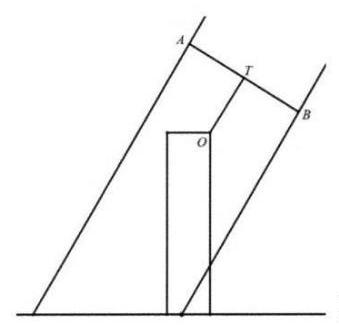
\includegraphics[max width=0.2\textwidth]{images/bo_d5jm9o77aajc7383vmi0_141_296_261_339_325_0.jpg}
\end{center}
\hspace*{3em} 

图 1

\begin{center}
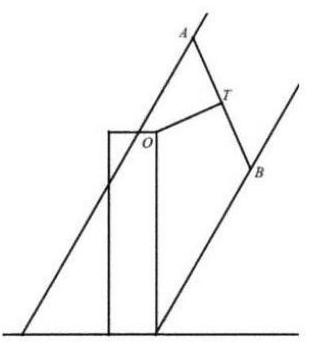
\includegraphics[max width=0.2\textwidth]{images/bo_d5jm9o77aajc7383vmi0_141_694_242_312_345_0.jpg}
\end{center}
\hspace*{3em} 

图 2

\begin{center}
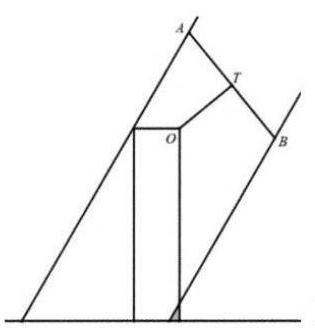
\includegraphics[max width=0.2\textwidth]{images/bo_d5jm9o77aajc7383vmi0_141_1066_256_315_332_0.jpg}
\end{center}
\hspace*{3em} 

(1)如图 3 在矩形“纸片人”上身恰好不被淋湿时，求其“裤脚”被淋湿 (阴影) 部分的面积 (结果精确到 \({0.1}{\mathrm{\;{cm}}}^{2}\) );

(2)请根据你的生活经验对小明建立的数学模型提两条改进建议(无需求解改进后的模型，如果建议超过两条仅对前两条评分).

【解析】(1) \(\frac{PO}{\sin \angle {PAO}} = \frac{AO}{\sin \angle {APO}}\) ,解得 \(\sin \angle {PAO} = \frac{\sqrt{6}}{6}\) ,

\(\cos \angle {DAB} = \sin \left( {{45}^{ \circ  } + \angle {PAO}}\right)  = \frac{\sqrt{3} + \sqrt{15}}{6}\) .

\begin{center}
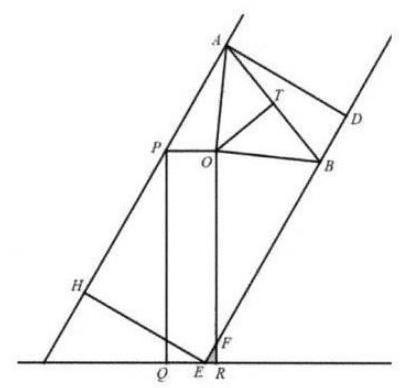
\includegraphics[max width=0.3\textwidth]{images/bo_d5jm9o77aajc7383vmi0_141_289_919_405_388_0.jpg}
\end{center}
\hspace*{3em} 

\({HE} = {AD} = {AB}\cos \angle {DAB} = {20}\left( {\sqrt{3} + \sqrt{15}}\right) .\)

\({ER} = \frac{170}{\sqrt{3}} + {40} - {20}\left( {\sqrt{3} + \sqrt{15}}\right) \frac{2}{\sqrt{3}} = \frac{170}{\sqrt{3}} - {40}\sqrt{5}\)

\({S}_{\bigtriangleup {EFR}} = \frac{\sqrt{3}}{2}E{R}^{2} \approx  {65.7}{\mathrm{\;{cm}}}^{2}.\)

(2)参考改进建议: \circled{1} 雨伞不遮挡视线；

 \circled{2} 伞面为弧形，改进模型将伞设为一段圆弧； \circled{3} 考虑伞柄可以伸缩；

 \circled{4} 人体改进为立体模型； \circled{5} 考虑风速、风向； \circled{6} 考虑撑伞的省力、稳定等。 只要合理，每条改进建议 2 分.
\end{document}